%%%%%%%%%%%%%%%%%%%%%%%%%%%%%%%%%%%%%%%%%%%%%%%%%%%%%%%%%%%%%%%%%%%%%%
% nuthesis-template.tex - Miguel A, Lerma - 3/31/2013
%                         mlerma@math.northwestern.edu
%%%%%%%%%%%%%%%%%%%%%%%%%%%%%%%%%%%%%%%%%%%%%%%%%%%%%%%%%%%%%%%%%%%%%%

%%%%%%%%%%%%%%%%%%%%%%%% DISCLAIMER %%%%%%%%%%%%%%%%%%%%%%%%%%%%%%%%%%
% 
% In spite of the effort to accommodate this template and the nuthesis
% class to the official requirements of the university to write a 
% Ph.D. dissertation, it is not possible to guarantee that it will 
% always work, and the author of the dissertation remains responsible
% for checking that such requirements are actually fulfilled by 
% his/her final work.
%
%%%%%%%%%%%%%%%%%%%%%%%%%%%%%%%%%%%%%%%%%%%%%%%%%%%%%%%%%%%%%%%%%%%%%%


\documentclass[12pt]{nuthesis}	% The nuthesis class is based on 
				% amsbook.cls.
\usepackage{graphicx}
\usepackage{amsmath}
\usepackage{achemso}
\usepackage{breqn}
\usepackage{bibentry}
\renewcommand{\vec}[1]{\mathbf{#1}} % Dan's addition - bold vectors.


%%%%%%%%%%%%%%%%%%%%%%%%%%%%%%%%%%%
% DATA OF AUTHOR AND DISSERTATION %
%%%%%%%%%%%%%%%%%%%%%%%%%%%%%%%%%%%

\author{Daniel C. Hannah}

\title{Spectroscopic and Computational Studies of Light and Heat Generation in Nanometer Scale Systems}

\degree{DOCTOR OF PHILOSOPHY}  % Default: DOCTOR OF PHILOSOPHY

\field{Chemistry}            % Default: Mathematics

\graduationmonth{July}         % The default is June or December
                                % depending on current date.

\graduationyear{2015}          % Default: current year.


				% Use \includeonly to select the 
%\includeonly{chap1,chap2,...}	% chapters to include if you are 
				% using the \include command below.
				% This way you can latex only a the 
				% part you are working on, which 
				% is faster than latexing the entire 
				% thesis. 

\setcounter{tocdepth}{3}% Include \subsubsection in ToC
\begin{document}
%	
%	THE BODY OF YOUR THESIS STARTS HERE
%

%%%%%%%%%%%%%%%%%%%%%%
% Some initial stuff %
%%%%%%%%%%%%%%%%%%%%%%

\frontmatter		% Preliminary pages start here.

\maketitle		% Produces the title page.

\copyrightpage		% Creates the copyright page.


\abstract		% Abstract.

For crystalline materials, the reduction of relevant material dimensions to the nanometer length scale often has a profound impact on the electronic, structural, optical, mechanical, and thermal properties.  

\acknowledgements	% Acknowledgements (optional).

Text for acknowledgments.

%\preface		% Preface (optional).

%This is the preface.



%% A few more optional pages (uncomment if needed)
%
%\listofabbreviations 
%
%This is the list of abbreviations (optional).
%
%\glossary
%
%This is the glossary (optional).
%
%\nomenclature
%
%This is the nomenclature (optional).
%
%% Note that the dedication text must be passed as an argument
%% of the \dedication command
\dedication{\emph{To my parents, who taught me the importance of loving what I do.}}
%

\clearpage\phantomsection % needed for the hyperlinks to work correctly
\tableofcontents	% Table of Contents will be automatically
			% generated and placed here.

\clearpage\phantomsection % needed for the hyperlinks to work correctly
\listoftables		% List of Tables and List of Figures will be placed

\clearpage\phantomsection % needed for the hyperlinks to work correctly
\listoffigures		% here, if applicable (optional).



\mainmatter             % Actual text starts here.

%%%%%%%%%%%%%%%%%%%%%%%%%%%
% Actual text starts here %
%%%%%%%%%%%%%%%%%%%%%%%%%%%

% If there is an introduction it must be the first chapter

\chapter{Introduction}	% The first Chapter.
Quantum-confined semiconductor nanocrystals (NCs) are crystalline clusters of atoms having a semiconductor composition with diameters smaller than the spatial extent of the electron and/or hole wavefunction in the corresponding bulk material. In this case, that particular carrier is said to be experiencing quantum confinement. While such materials are also commonly referred to as quantum dots, we refer to this material class (colloidal, quantum confined semiconductor nanocrystals) as NCs to distinguish them from the various other types of quantum dots common in the literature, such as epitaxial self-assembled quantum dots or gate-defined quantum dots. In this thesis, we focus on cluster sizes and materials for which \emph{both} carriers are strongly confined. In general, NCs exhibit size-dependent, broadly tunable absorption and emission spectra, near-unity quantum yields, and are amenable to low-cost, easily scalable solution-phase processing. Furthermore, they exhibit emergent physical processes such as hot electron transfer and carrier multiplication. As a result, they have been suggested as a means to improve a wide variety of energy-relevant technologies including LEDs, lasers, solar cells, transistors, and thermoelectric power converters. Since their initial synthesis in 1985, the optical and electronic properties of NCs have received a great deal of attention, and a great deal is now understood regarding the electronic structure of this fascinating material class. We review some important aspects of NC electronic structure and optical properties here. As the work presented in this thesis is concerned with nanoscale energy generation and dissipation, we also review the basics of phonon-assisted carrier cooling and thermal transport.

\section{Quantum Confinement and Electronic Structure}
\subsection{Particle-in-a-Sphere}
The remarkable effects of quantum confinement are most easily understood by considering the NC as a particle-in-a-sphere \cite{efros1982interband, brus1986electronic}, analogous to the particle-in-a-box problem familiar from quantum mechanics. We will begin by applying spherical boundary conditions to a bulk semiconductor wavefunction. The spherical boundary conditions applied here take the form of an infinite spherical potential of radius $a$, $V(\vec{r})$, such that:
\begin{equation}\label{eq:pis1}
V(\vec{r}) = \left\{
	\begin{array}{ll}
		0 & \mbox{if } \vec{r} < a \\
		\infty & \mbox{if } \vec{r} > a
	\end{array}
\right.
\end{equation}

As a starting point, we utilize Bloch's theorem, which states that in a perfectly crystalline and periodic material, we may write the carrier wavefunction as the product of a wavelike portion and a cell-periodic portion, as shown below:
\begin{equation}\label{eq:pis2}
\Psi_{n\vec{k}}(\vec{r}) = u_{n\vec{k}}e^{i\vec{k}\cdot\vec{r}}
\end{equation}
In Equation \ref{eq:pis2}, the function $u_{n\vec{k}}$ is a function with the periodicity of the crystal lattice, with the wavefunctions being labeled by band index $n$ and wavevector $\vec{k}$. Eigenvalues of the Schr{\"o}dinger equation for Eq. \ref{eq:pis2} yield an energy spectrum of the form:
\begin{equation}\label{eq:pis3}
E_{n}\left(\vec{k}\right) = \frac{\hbar^2\vec{k}_n^2}{2m_{\mathrm{eff}}}
\end{equation}
In Eq. \ref{eq:pis3} we have utilized the so-called effective mass approximation, in which semiconductor carriers behave as free particles but with an altered ("effective") mass compensating for the complex potential experienced by the carriers due to the host lattice. In the effective mass approximation, the valence and conduction bands are assumed to have parabolic forms, evident in the $\vec{k}^2$ dependence of the energy levels (Eq. \ref{eq:pis3}) and demonstrated graphically in Figure \ref{f:pis1}. \par

\begin{figure}
\begin{center}
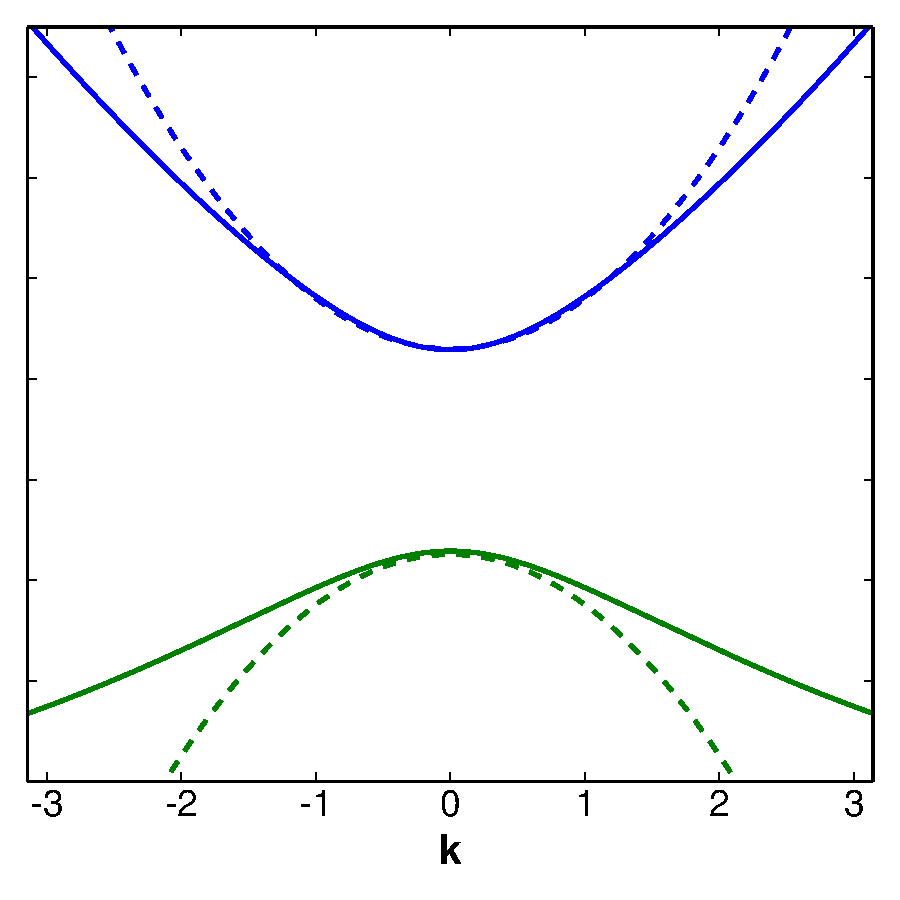
\includegraphics[width=0.5\textwidth]{./Chapter1/parabolic.pdf}
\caption[Two-band model for a direct gap semiconductor in the parabolic band approximation.]{Two-band model for a direct gap semiconductor in the parabolic band approximation. The true band structure is shown in solid lines, while the parabolic bands, centered at $\vec{k} = 0$ utilized in the effective mass approximation are shown in dashed lines.}
\label{f:pis1}
\end{center}
\end{figure}

To satisfy the spherical boundary condition, the single-particle (i.e. electron or hole) wavefunction is written as a linear combination of Bloch wavefunctions (Eq. \ref{eq:pis2}):
\begin{equation}\label{eq:pis4}
\Psi_{sp}\left(\vec{r}\right) = u_{n0}\left(\vec{r}\right)\sum_{\vec{k}}C_{n\vec{k}}e^{i\vec{k}\cdot\vec{r}}
\end{equation}
In Eq. \ref{eq:pis4}, we have assumed no dependence of $u$ on $\vec{k}$, implying a tight-binding approximation and allowing the function $u$ to be written as a sum of atomic wavefunctions $\{\phi\}$, i.e. $u_n \approx \sum_{i} C_{ni}\phi_n\left(\vec{r} - \vec{r_i}\right)$ where $i$ indexes the lattice sites. This reduces the problem to the determination of the envelope functions, $f_{sp}\left(\vec{r}\right) = \sum_{\vec{k}}C_{n\vec{k}}e^{i\vec{k}\cdot\vec{r}}$, which enforce the spherical symmetry. These envelope functions can be calculated by solving the Schr{\"o}dinger equation for an arbitrary particle in a spherical confining potential (Eq. \ref{eq:pis1}). This yields wavefunctions of the form:
\begin{equation}\label{eq:pis5}
\Phi_{n,l,m}\left(r,\theta, \phi\right) = C\frac{j_l\left(k_{n,l},\vec{r}\right)Y_l^m\left(\theta,\phi\right)}{r}
\end{equation}
In Eq. \ref{eq:pis5}, $Y_l^m\left(\theta,\phi\right)$ is a spherical harmonic function, $j_l\left(k_{n,l},\vec{r}\right)$ is the $l$th order spherical Bessel function, and $k_{n,l} = \alpha_{n,l}/a$, where $\alpha_{n,l}$ is the $n$th zero of $j_l$. Plugging the functions $\Phi$ directly in for the envelope functions $f_{sp}$, we arrive at the electron-hole pair states:
\begin{equation}\label{eq:pis6}
\begin{split}
\Psi_{e-h}\left(\vec{r}_e, \vec{r}_h\right) &= \Psi_e\left(\vec{r}_e\right)\Psi_h\left(\vec{r}_h\right) = u_ef_e\left(\vec{r}_e\right)u_hf_h\left(\vec{r}_h\right) \\
&= C\left[u_e\frac{j_{Le}\left(k_{ne,Le},\vec{r}_e\right)Y_l^m\left(\theta,\phi\right)}{r}\right]\left[u_h\frac{j_{Lh}\left(k_{nh,Lh},\vec{r}_h\right)Y_l^m\left(\theta,\phi\right)}{r}\right]
\end{split}
\end{equation}
Solving for the eigenvalues associated with these wavefunctions and adding offsets to account for the bulk semiconductor band gap ($E_g$) and Coulomb interaction of the electron and hole ($E_c$) yields the energy eigenvalues for the electron-hole pairs:
\begin{equation}\label{eq:pis7}
E_{e-h} \left(n_h, L_h, n_e, L_e\right) = E_g + \frac{\hbar^2}{2a^2}\left(\frac{\alpha_{nh, Lh}^2}{m_{\mathrm{eff}}^h} + \frac{\alpha_{ne, Le}^2}{m_{\mathrm{eff}}^e}\right) - E_c
\end{equation}
In Eqs. \ref{eq:pis6} and \ref{eq:pis7}, the quantum states are labeled by the quantum numbers $n_h, L_h, n_e$, and $L_e$. While the bookkeeping begins to become cumbersome, Eqs. \ref{eq:pis6} and \ref{eq:pis7} reveal some important basic features of NC electronic structure. Firstly, the enforcement of spherical boundary conditions leads to a quantization of the wavevector $k$, yielding a discrete, molecule-like density of states. Figure \ref{f:pis2} graphically depicts the quantization of $k$ values and resulting set of discrete transitions. Furthermore, the dependence of $E_{e-h}$ on $a^{-2}$ reveals the strongly size-dependent energy spectra characteristic to NCs. Finally, it is worth noting that the simple treatment of electron-hole Coulomb attraction as a first-order correction to the energy is justified in this case: Confinement energy ($\propto a^{-2}$) overwhelms the Coulomb interaction ($\propto a^{-1}$) in the strong confinement regime. It is worth noting that while the term "exciton" is occasionally used in this thesis to refer to NC electron-hole pairs, this terminology is used loosely with the full understanding that these excitons are most strongly bound by spatial confinement rather than Coulombic attraction, in contrast to the excitons found in bulk materials. Still, theoretical treatments of the strongly-confined electron-hole pair as a single exciton quasiparticle have been found to be effective for describing many properties of interest \cite{scholes2006excitons}. \par

\begin{figure}
\begin{center}
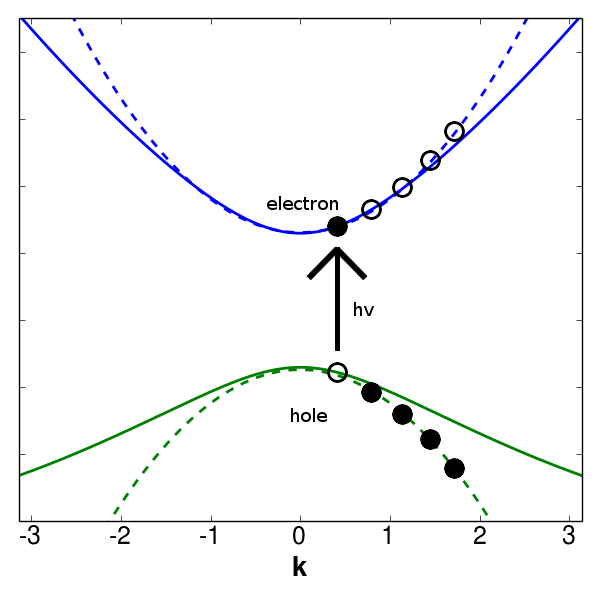
\includegraphics[width=0.5\textwidth]{./Chapter1/parabolic_quantized.png}
\caption[Discrete energy spectrum in a two-band model due to spherical confinement.]{Discrete energy spectrum in a two-band model due to spherical confinement. Imposing a spherical confining potential on the bulk Bloch wavefunctions results in $k$ quantization, with each electron/hole shown in the figure representing a quantized $k$ state.}
\label{f:pis2}
\end{center}
\end{figure}

\subsection{Exciton Fine Structure}
While the particle-in-a-sphere model is useful for understanding the physical origins of discrete transitions and size-dependent optoelectronic properties in NCs, the band structure of real semiconductor compositions is significantly more complicated. As an example, CdSe, an archetypal semiconductor nanocrystal composition, is a $sp^3$ hybridized semiconductor exhibiting the wurtzite crystal structure. Se $4p$ orbitals form the valence band, while Cd $5s$ orbitals form the conduction band. As both Cd and Se are relatively heavy elements, CdSe NCs exhibit strong spin orbit coupling, which splits the valence band into a fourfold degenerate band maximum and a split-off sub-band. Another consequence of this strong spin-orbit coupling is that only the total angular momentum of a state $F$ (spin + orbital momentum) is a good quantum number. Because excited electrons occupy $s$ orbitals, they exhibit $F_{\mathrm{electron}} = \pm1/2$, while valence band ($p$-orbital) holes may exhibit $F_{\mathrm{hole}} = \pm3/2$ or $\pm1/2$. Therefore an electron-hole pair may have $F = \pm2, \pm1$ or 0. The lowest excitonic state of CdSe NCs presents eight fine structure states, two having $F = \pm2$, four having $F= \pm1$, and two having $F = 0$. Figure \ref{f:efs1} displays a schematic of this excitonic state in terms of the exciton fine structure described here. \par

\begin{figure}
\begin{center}
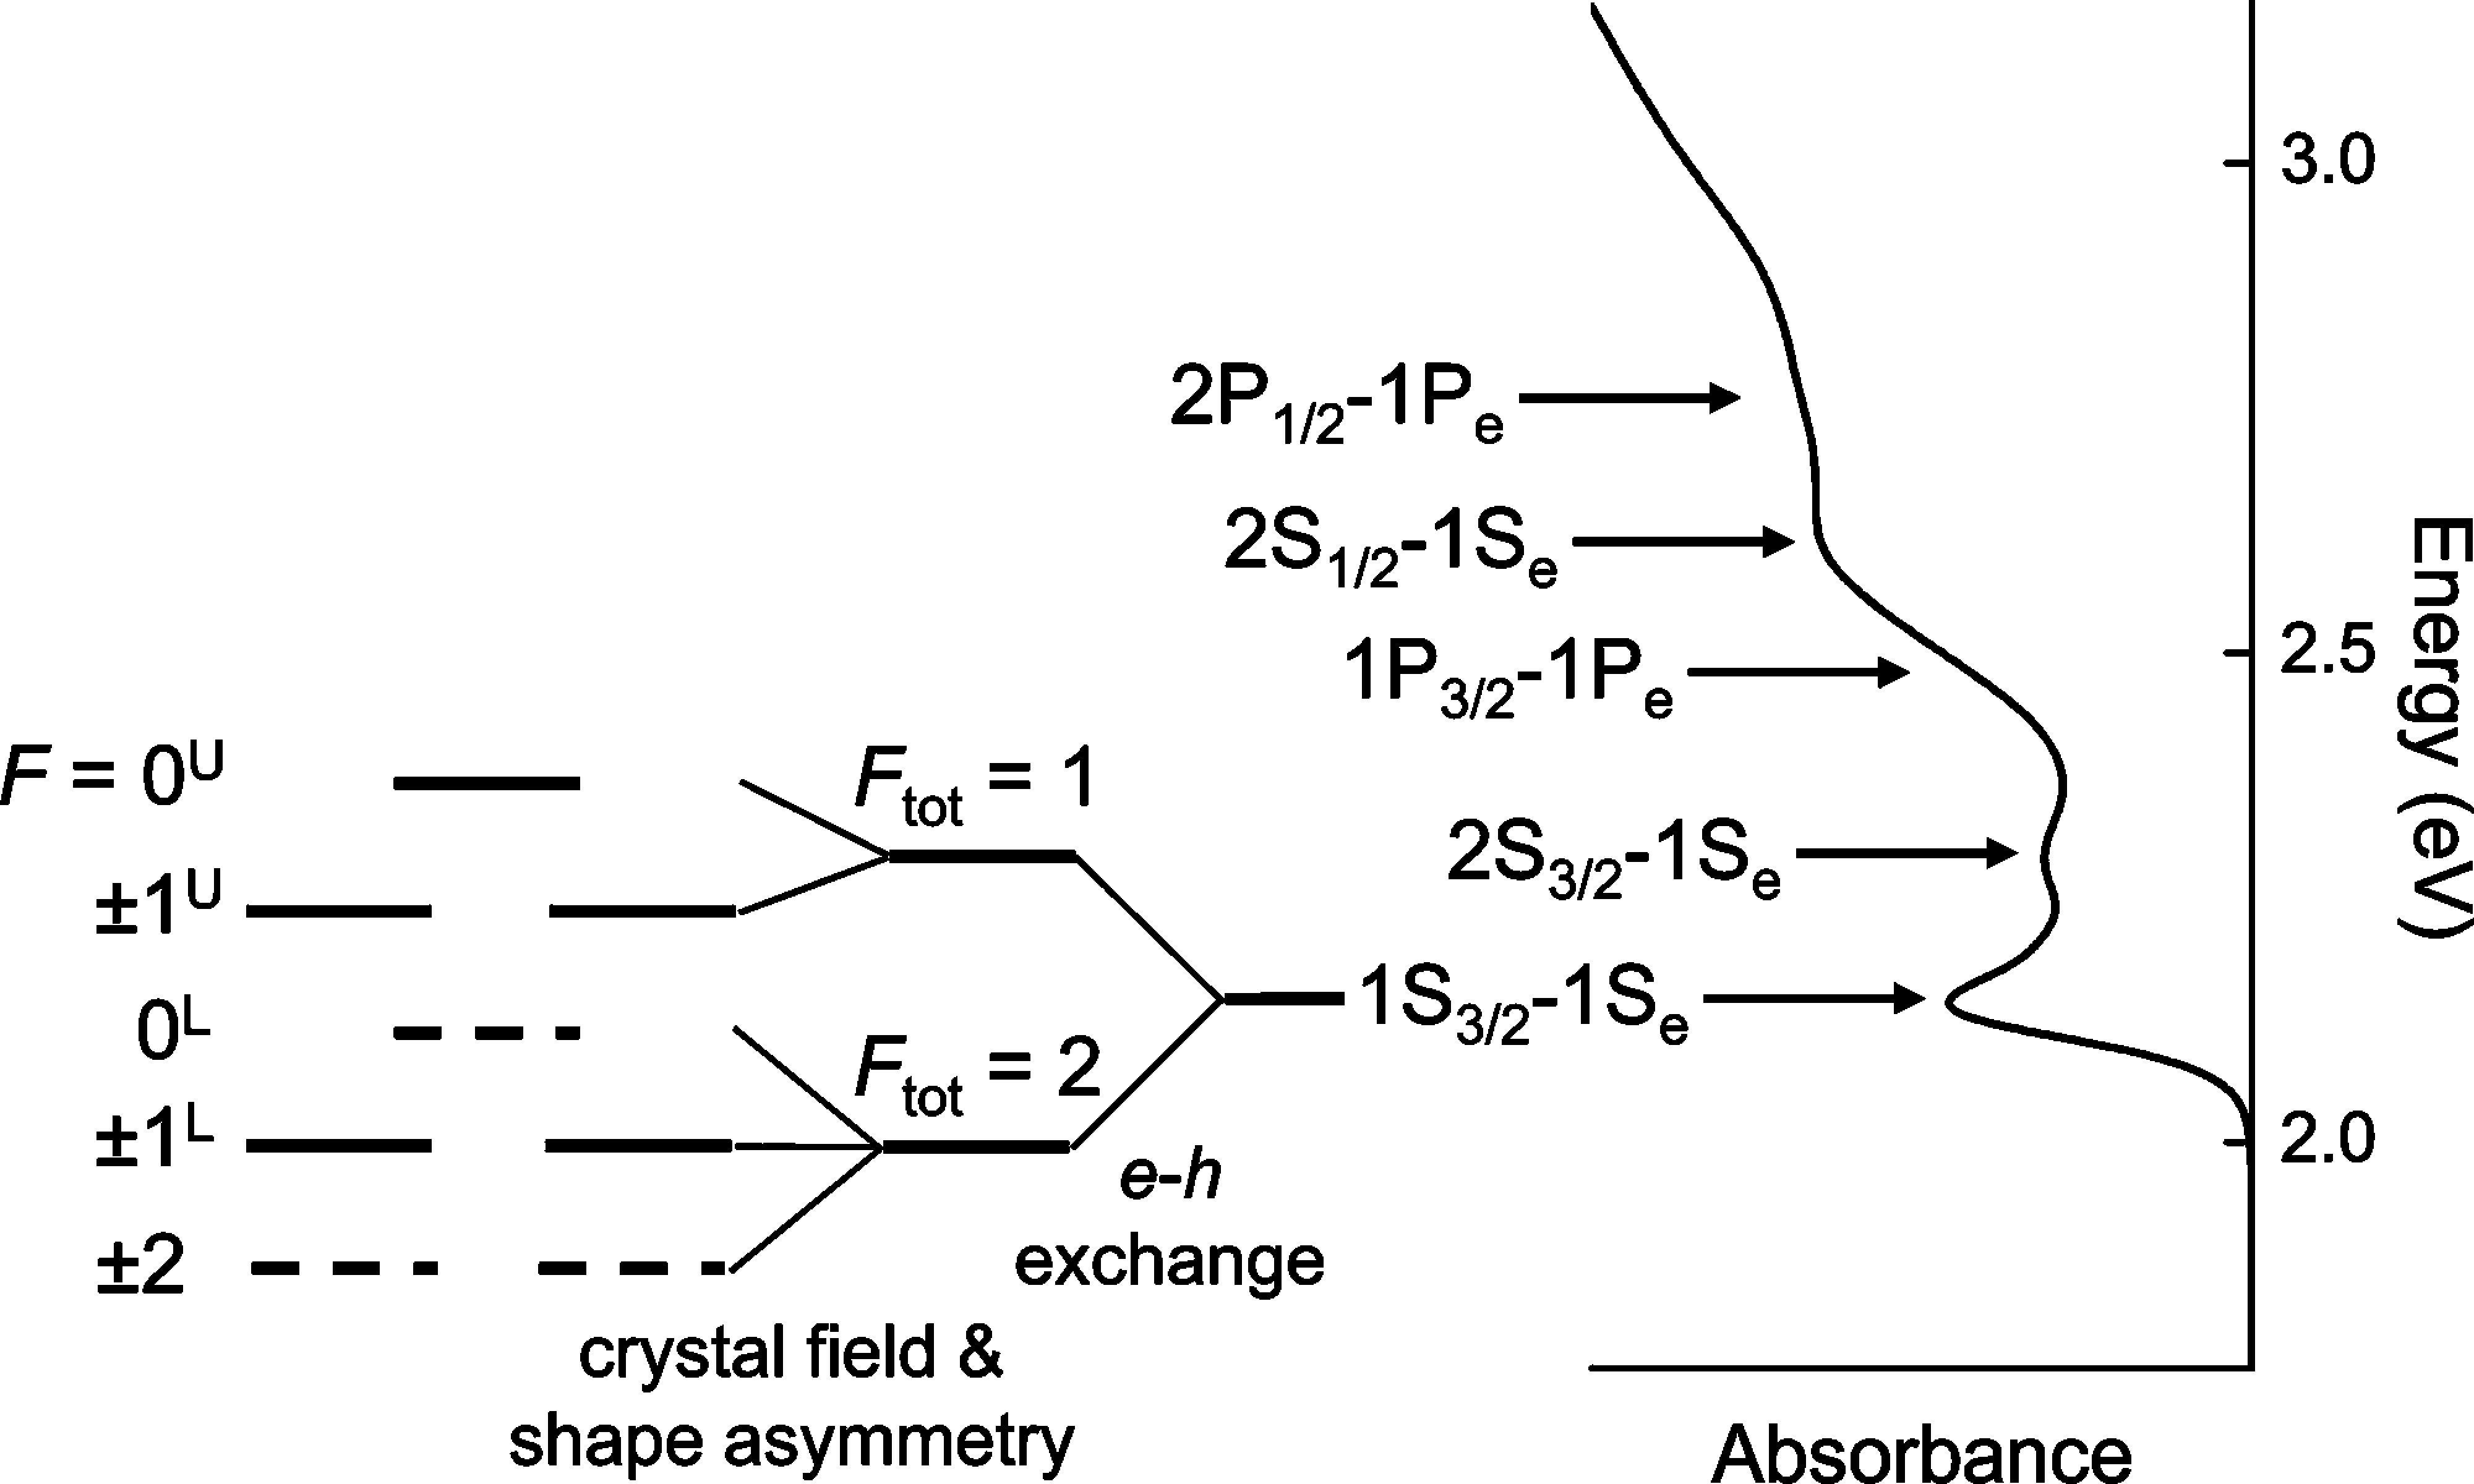
\includegraphics[width=\textwidth]{./Chapter1/efs_scholes.jpeg}
\caption[Exciton fine structure of CdSe nanocrystals]{Optical absorption spectrum of CdSe NCs (right hand side) with the first sharp absorption peak, due to the lowest-energy excitonic state $1S_{3/2}-1S_e$, labeled according to its exciton fine structure states \cite{kim2009exciton}.}
\label{f:efs1}
\end{center}
\end{figure}

Another consequence of spatial confinement is that the exchange interaction between electrons and holes become greatly enhanced. In brief, the exchange interaction causes the splitting of degenerate configurations into bright ($F = \pm1$ or $0$) and dark ($F = \pm2$) states. The dark states are so named because they cannot interact with photons (which cannot carry an angular momentum of 2) in the dipole approximation. Finally, the effect of the wurtzite crystal field must be considered. Because the wurtzite structure is asymmetric, the crystal field splits the valence band into two energy levels ($F_{\mathrm{hole}} = \pm3/2$ and $F_{\mathrm{hole}} = \pm1/2$) (because the $p$-orbitals do not each experience the same crystal field). Taken together, the exciton fine structure shown on the left hand side of Figure \ref{f:efs1} results. \par

The notions of electron-hole exchange interaction and splitting due to the wurtzite crystal field have been accounted for mathematically in the context of multiband effective mass theory in a landmark paper by Efros and co-workers \cite{PhysRevB.54.4843}. While the mathematical details are beyond the scope of the Chapter, one extremely important result is relayed here, shown in Figure \ref{f:efs2}. 

\begin{figure}
\begin{center}
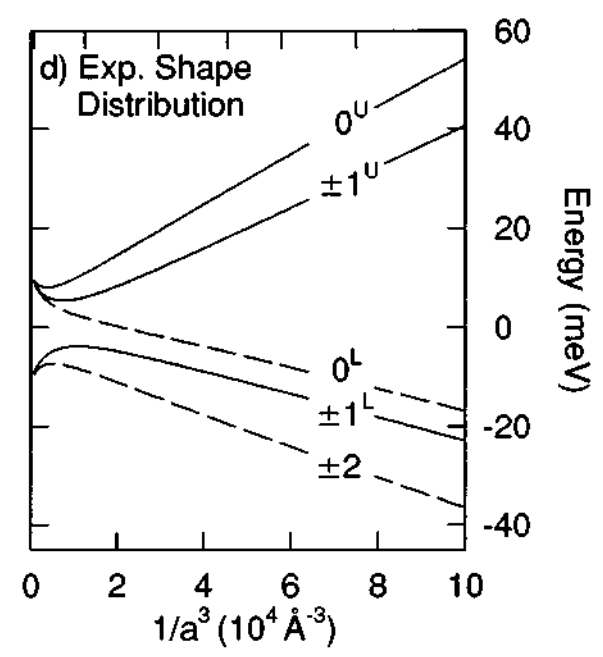
\includegraphics[width=0.5\textwidth]{./Chapter1/efs_efros.png}
\caption[Size-dependence of exciton fine structure in CdSe nanocrystals.]{Size-dependence of the exciton fine structure for the $1S_{3/2}-1S_e$ (band edge) exciton in CdSe NCs. Reproduced from the work by Efros \emph{et al.} \cite{PhysRevB.54.4843}, who utilized a multiband effective mass model with sizes and shape asymmetry derived from experimental measurements.}
\label{f:efs2}
\end{center}
\end{figure}

As shown in Figure \ref{f:efs2}, the splitting between exciton fine structure states in CdSe nanocrystals depends on NC size, a result which has been predicted theoretically and experimentally confirmed using low-temperature optical measurements \cite{PhysRevB.54.4843}. The implications of the exciton fine structure in CdSe are discussed further in Chapter 3.

\section{Carrier Cooling in Semiconductor Nanocrystals}

The intraband relaxation of excited charge carriers in semiconductor NCs has been a topic of significant interest owing to the theoretical prediction of dramatically slowed carrier cooling rates in comparison to bulk materials \cite{benisty1991intrinsic, bockelmann1990phonon}. In bulk semiconductors, intraband relaxation of hot carriers occurs on a roughly 1 ps timescale. This cooling occurs so rapidly due to the continuous energy bands exhibited by bulk, crystalline materials, which provide resonant electronic states for highly efficient electron-phonon scattering.  A general schematic of the carrier cooling process is displayed in Figure \ref{f:carrier_cooling1} \cite{nozik2001spectroscopy}. 

\begin{figure}
\begin{center}
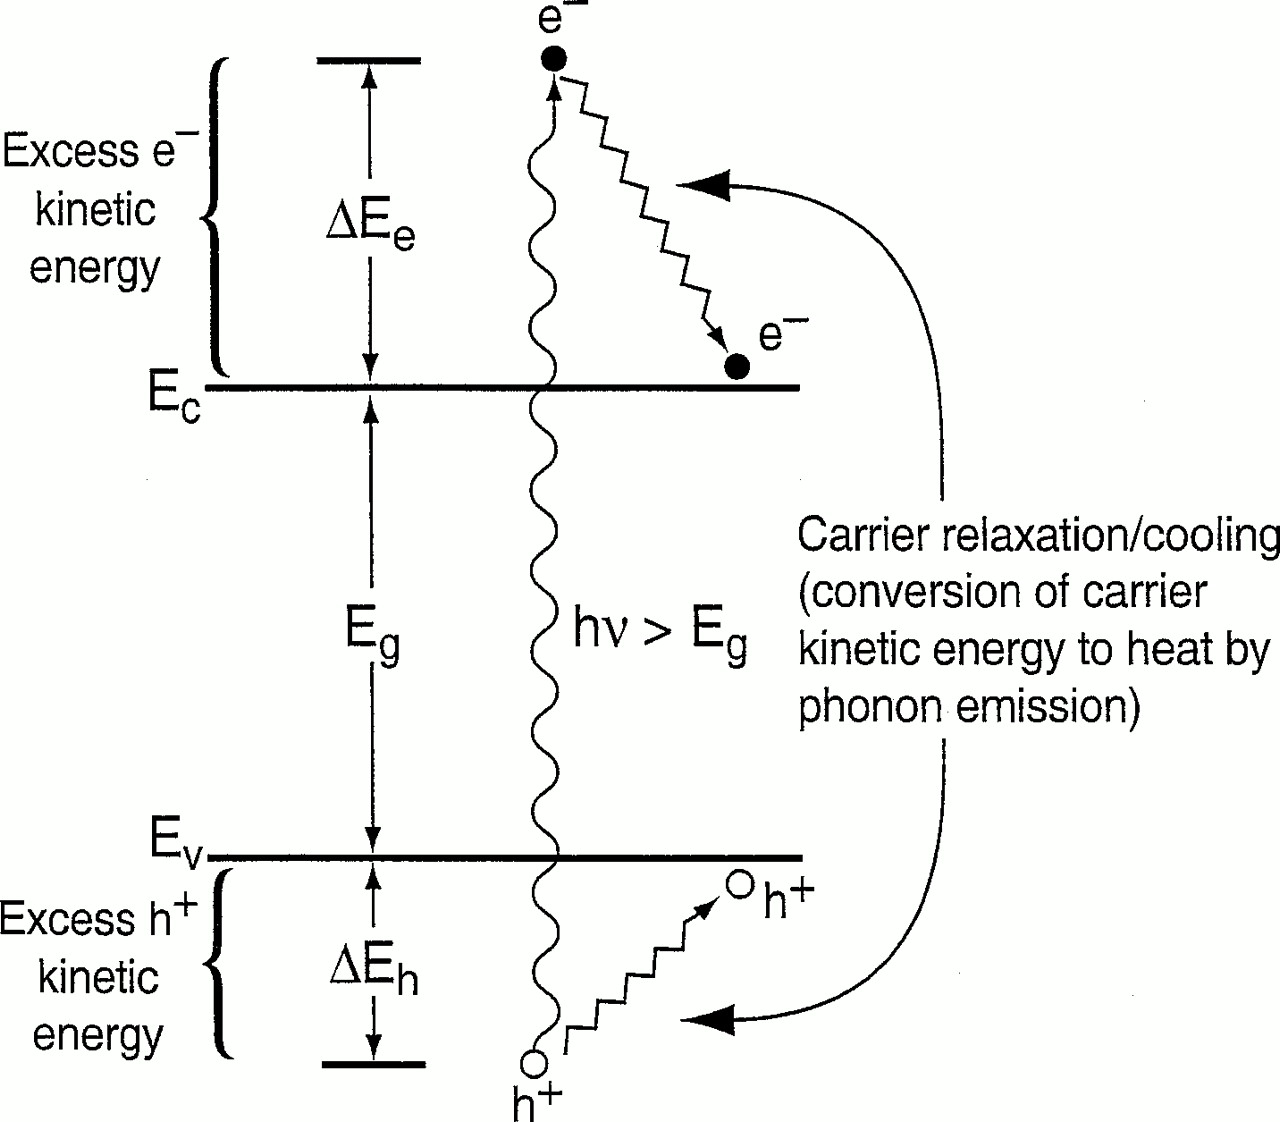
\includegraphics[width=0.5\textwidth]{./Chapter1/carrier_cooling.jpeg}
\caption[Schematic of phonon-assisted intraband carrier cooling in semiconductors.]{Subsequent to the creation of highly excited electrons and holes by absorption of an above gap photon, charge carriers relax to the conduction and valence band extrema ($E_c$ and $E_v$, respectively) by emitting phonons and heating the semiconductor lattice.}
\label{f:carrier_cooling1}
\end{center}
\end{figure}

In NCs, the discrete density of states arising from quantum confinement creates a scenario where the energetic spacing can exceed 10 times the LO phonon energy (typically on the order of $\sim$25 meV), which suggests that multi-phonon emission would be required to enable carrier relaxation. Such a multi-particle process would be much less efficient than cooling facilitated by single phonon emission, leading to the expectation of a "phonon bottleneck" with intraband carrier relaxation possibly taking up to a microsecond \cite{bockelmann1990phonon}. The prospect of a phonon bottleneck is enticing, as slowed carrier potentially offers benefits to many energy-related technologies. In particular, the ability to harvest hot carriers in photovoltaic cells would permit the utilization of above-gap solar photons to generate additional voltage. Alternatively, slowed carrier cooling would likely also benefit carrier multiplication processes, providing additional current. \par

Despite predictions of slowed carrier thermalization and the potential benefits of such a phenomenon, transient absorption measurements of carrier cooling relay subpicosecond-to-picosecond intraband relaxation times comparable to those exhibited by bulk materials \cite{PhysRevB.60.R2181, PhysRevLett.80.4028,PhysRevLett.96.057408}. Such rapid carrier transfer in NCs begins to suggest the involvement of other highly efficient relaxation processes, such as electron-to-hole energy transfer or energy transfer to surface-bound organic ligands exhibiting higher frequency vibrations \cite{pandey2008slow, guyot2005intraband}.\par

\begin{figure}
\begin{center}
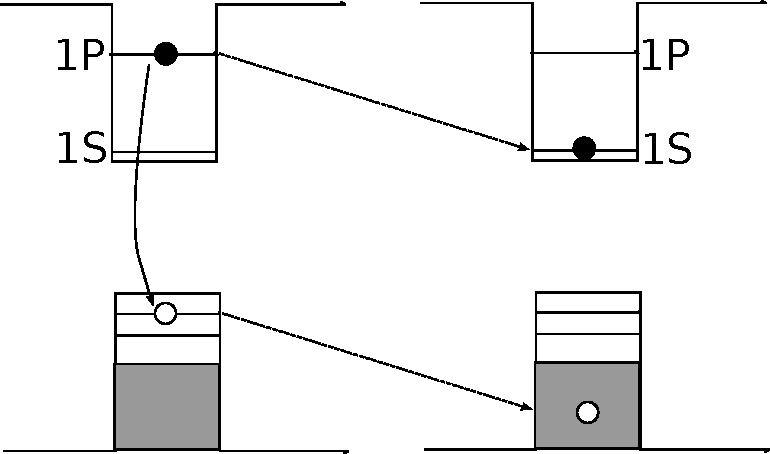
\includegraphics[width=0.5\textwidth]{./Chapter1/auger.pdf}
\caption[Schematic of Auger-like electron-to-hole energy transfer in NCs.]{Confinement enhanced, Auger-like energy transfer in NCs entails a highly excited electron (solid circle) resonantly transfering energy to the hole (open circle) \emph{via} the Coulomb interaction. This facilitates rapid electron cooling even in the presence of conduction band states with energetic separation well in excess of typical phonon energies. Holes, which are heavier, can still undergo phonon-assisted relaxation through the valence band.}
\label{f:carrier_cooling2}
\end{center}
\end{figure}

The dominant mechanism for rapid carrier cooling in NCs is theorized to be Auger-like energy transfer from the electron to the hole, which proceeds in the following fashion. Electrons, typically exhibiting a smaller effective mass than the hole, resonantly transfer energy uni-directionally \emph{via} a Coulombic interaction to holes. Subsequent to this energy transfer, the heavier holes, which experience a higher density of states, efficiently couple to phonons to relax to the band edge. Figure \ref{f:carrier_cooling2} graphically depicts the Auger-like energy transfer process, with the hole being excited into a "bulk"-like quasi-continuum of states at high energies, shown as a solid grey section of the valence band in the figure. While the theoretically predicted Auger-like energy transfer rates exhibit a size-dependence matching experimentally measured intraband relaxation times in NCs, the theory ultimately remains unproven, with more recent experimental results possibly challenging this interpretation. We explore this notion in detail in Chapter 2.

\section{Mechanisms of Heat Transport}
Another major focus of this thesis is the ultimate fate of phonons after they are generated by intraband carrier thermalization (and other means). As NCs become increasingly technologically relevant, it will become necessary to address the thermal management challenges inherent to this material class. While NCs exhibit remarkable, tunable optical and electronic properties, they present a greatly elevated surface-to-volume ratio which depresses the melting point relative to bulk materials \cite{goldstein1992melting}. Furthermore, even at temperatures below the NC melting point, processing such as sintering in NC films can alter the size-dependent optical properties and negatively affect performance \cite{drndic2002transport}. Finally, the chemical passivating layer on the surface renders NCs susceptible to damage mechanisms such as ligand decomposition and subsequent surface trap formation. \par

NCs and films comprised of them present unique challenges with regard to the study of thermal transport. Addressing some of these challenges is the focus of Chapter 3 of this thesis, and we elaborate on many NC-specific challenges there. Here, we review some of the basic theory of thermal transport in order to lay a foundation for the work presented in this thesis.

\subsection{Fourier's Law}
Heat conduction is an energy transfer process through a medium which is caused by a temperature difference due to the motion of heat carriers in that medium. Importantly, heat conduction requires a medium, and such processes are usually modeled on the basis of Fourier's Law \cite{chen2000particularities}:
\begin{equation}\label{eq:fourier1}
q = -\lambda\nabla T
\end{equation}
In Equation \ref{eq:fourier1}, $q$ is the heat flux, $\nabla T$ is the temperature gradient, and $\lambda$ is the thermal conductivity. Fourier's Law implicitly assumes diffusive heat transport mediated by the scattering of heat carriers in the material (phonons in semiconductors and insulators, while in metals electrons also exhibit significant heat capacity). Applying this theory to systems exhibiting structure or grain boundaries on the nanometer length scale is challenging, as typical phonon mean free paths exceed this length scale significantly \cite{chen2000particularities, cahill2003nanoscale}. As a result, one might intuitively expect shorter distances between scattering events as compared to bulk materials and commensurately reduced thermal conductivity. Indeed, this is generally the case \cite{cahill2003nanoscale}, and nanostructuring has emerged as a major paradigm in the rational design of thermoelectric materials exhibiting ultralow thermal conductivity \cite{doi:10.1021/cm902195j, Hsu06022004}. \par
Development of a complete model of nanoscale heat transport remains an extremely active area of research \cite{cahill2014nanoscale, france2014atomistic, merabia2014thermal, maznev2015boundary}. As we will see, even thermal transport at isolated, chemically-passivated interfaces presents significant outstanding experimental and theoretical challenges. As a starting point, it is reasonable to consider heat transport at an interface, as it is interfacial scattering which dominates heat transport in nanoscale systems. Extending Fourier's Law, we may write:
\begin{equation}\label{eq:fourier2}
q = G\Delta T
\end{equation}
In Eq. \ref{eq:fourier2}, $G$ is the interfacial thermal conductance and $\Delta T$ is the temperature change at the interface. Next, we present a microscopic theory of $G$ and comment on the difficulties associated with the analytical calculation of this term, highlighting the need for numerical simulations.

\subsection{Heat Transport at Interfaces}
As described above, systems presenting interfaces on length scales much less than typical phonon mean free paths will usually exhibit thermal transport dominated by interfacial thermal conductance. A theoretical model of interfacial thermal conductance begins with a microscopic expression for phonon flux at an interface. Figure \ref{f:ch1nano1} displays a diagram of the interface between two materials.

\begin{figure}
\begin{center}
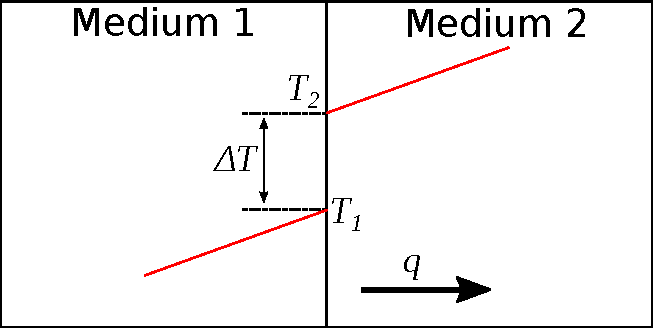
\includegraphics[width=0.5\textwidth]{./Chapter1/nanoscale1.pdf}
\caption[Diagram of thermal transport between interfaces.]{Model of interfacial thermal conductance \cite{PhysRevB.86.094303}. The red lines represent temperature profiles in each material, with a temperature jump shown at the interface. This discontinuity arises from different thermal conductivity in each material. The interfacial heat flux is given by $q$, and the direction of this flux by the arrow in medium 2.}
\label{f:ch1nano1}
\end{center}
\end{figure}

In the most general sense, we may naively write the following expression for phonon flux in the $z$ direction for an interface between two material regions designated $L$ and $R$ (Medium 1 and 2, respectively, in Fig. \ref{f:ch1nano1}) \cite{PhysRevB.80.165304}:
\begin{equation}\label{eq:nanoheat1}
\begin{split}
q =& \frac{1}{\left(2\pi\right)^3}\left[\int_L\sum_v^+ \hbar\omega(\vec{k},v)v_z(\vec{k}, v)\alpha_{L \rightarrow R}(\vec{k},v)f_L(\vec{k},v)\mathrm{d}\vec{k}\right. \\
&+ \left.\int_R\sum_v^- \hbar\omega(\vec{k},v)v_z(\vec{k}, v)\alpha_{R \rightarrow L}(\vec{k},v)f_R(\vec{k},v)\mathrm{d}\vec{k}\right]
\end{split}
\end{equation}

Equation \ref{eq:nanoheat1} simply sums up, for each phonon polarization (or vibrational mode $v$ in a molecular eigenstate picture) $v$, the energy of a phonon having frequency $\omega$ multiplied by its velocity in the $z$ direction, $v_z$, an energy-dependent transmission coefficient $\alpha$ (with energy-dependence entering via the dependence on phonon wavevector $\vec{k}$), and a phonon distribution function $f$, which accounts for thermal population of the various modes. Each sum is integrated over the first Brillouin zone of that particular lead ($L$ or $R$). The factor $1/\left(2\pi\right)^3$ accounts for the reciprocal space volume in the medium.  Given exact forms of the transmission coefficient and the phonon distribution function, this expression for phonon flux is exact, however, exact expressions for these terms are difficult to obtain for heterogeneous interfaces. Varying levels of approximiations exist, the most relevant of which we will describe here, along with specific issues related to nanoscale thermal transport.\par

The most straightforward approximation is to model the phonon distribution function, $f$, with the equilibrium Bose-Einstein distribution, i.e.:
\begin{equation}\label{eq:nanoheat2}
f_{L/R} = f_{eq}(\omega, T) = \frac{1}{e^{-\hbar\omega/k_BT} - 1}
\end{equation}
In Eq. \ref{eq:nanoheat2}, $k_B$ is Boltzmann's constant and $T$ is temperature. The use of an equilibrium distribution function to describe an inherently non-equilibrium process (heat transport) leads to the significant contradiction that the interface between two identical materials is predicted to have a finite interfacial thermal conductance. To demonstrate this, we note that flux must vanish at equilibrium, i.e. $q = 0$. Then, the two terms on the right-hand side of Eq. \ref{eq:nanoheat1} must vanish:
\begin{equation}\label{eq:nanoheat3}
\begin{split}
\int_L\sum_v^+ \hbar\omega(\vec{k},v)v_z(\vec{k}, v)\alpha_{L \rightarrow R}(\vec{k},v)f_{eq}(\omega, T_L)\mathrm{d}\vec{k} \\
= -\int_R\sum_v^- \hbar\omega(\vec{k},v)v_z(\vec{k}, v)\alpha_{R \rightarrow L}(\vec{k},v)f_{eq}(\omega, T_R)\mathrm{d}\vec{k}
\end{split}
\end{equation}
We can then simplify Eq. \ref{eq:nanoheat1} to involve integration over only one side of the interface:
\begin{equation}\label{eq:nanoheat4}
q = \frac{1}{\left(2\pi\right)^3}\int_L\sum_v^+ \hbar\omega(\vec{k},v)v_z(\vec{k}, v)\alpha_{L \rightarrow R}(\vec{k},v)\left[f_{eq}(\omega, T_L) - f_{eq}(\omega, T_R)\right]\mathrm{d}\vec{k}
\end{equation}
Using Fourier's Law (described in the previous section), this can be converted to an interfacial thermal conductance.
\begin{equation}\label{eq:nanoheat5}
G = \frac{q}{T_L - T_R} = \frac{1}{\left(2\pi\right)^3}\int_L\sum_v^+ \hbar\omega(\vec{k},v)v_z(\vec{k}, v)\alpha_{L \rightarrow R}(\vec{k},v)\left[\frac{f_{eq}(\omega, T_L) - f_{eq}(\omega, T_R)}{T_L - T_R}\right]\mathrm{d}\vec{k}
\end{equation}
In the equilibrium limit, $T_L \rightarrow T_R$, and we arrive at the Landauer interfacial thermal conductance \cite{landauer1970electrical}:
\begin{equation}\label{eq:nanoheat6}
G_{eq} = \frac{1}{\left(2\pi\right)^3}\int_L\sum_v^+ \hbar\omega(\vec{k},v)v_z(\vec{k}, v)\alpha_{L \rightarrow R}(\vec{k},v)\left[\frac{\partial f_{eq}\left(\omega, T_R\right)}{\partial T}\right]\mathrm{d}\vec{k}
\end{equation}
As noted above, Eq. \ref{eq:nanoheat6} predicts a \emph{finite} thermal conductance between identical materials ($\alpha_{L \rightarrow R} = 1$), which is clearly unphysical. To address this issue, we may utilize the Boltzmann transport equation under relaxation time approximation (RTA), which gives an expression for the non-equilibrium phonon distribution function \cite{ziman1960electrons}.  In the RTA, the time dependence of the phonon distribution function, $f$, is given by Equation \ref{eq:nanoheat7}:
\begin{equation}\label{eq:nanoheat7}
\frac{\partial f_i}{\partial t} + v_i \cdot \nabla f_i = \frac{f_i - f_{eq}}{\tau_i\left(\omega\right)}
\end{equation}
In Eq. \ref{eq:nanoheat7}, $\tau_i$ is the mode-dependent relaxation time, which is a measure of the time taken for a non-equilibrium phonon population to return to its equilibrium state. A solution of this differential equation is given by Equation \ref{eq:nanoheat8}:
\begin{equation}\label{eq:nanoheat8}
f_i\left(\vec{r}\right) = f_{eq}\left[T(\vec{r})\right] - \tau_i\left(\frac{\partial f_{eq}}{\partial T}\right)v_i \cdot \nabla T
\end{equation}
Inserting the new distribution function (Eq. \ref{eq:nanoheat8}) into the expression for flux (Eq. \ref{eq:nanoheat1}) and grouping the terms into equilibrium and non-equilibrium branches, we have:
\begin{equation}\label{eq:nanoheat9}
\begin{split}
q &= G_{eq} \cdot (T_L - T_R) - \int_L\sum_{v}^{+}\hbar\omega(\vec{k},v)v_z(\vec{k},v)^2\alpha_{L\rightarrow R}(\vec{k},v)\tau_L\left(\frac{\partial f_{eq}}{\partial T}\right)\left(\frac{\partial f_{eq}}{\partial z}\right)_L \\
&- \int_R\sum_{v}^{+}\hbar\omega(\vec{k},v)v_z(\vec{k},v)^2\alpha_{R\rightarrow L}(\vec{k},v)\tau_R\left(\frac{\partial f_{eq}}{\partial T}\right)\left(\frac{\partial f_{eq}}{\partial z}\right)_R
\end{split}
\end{equation}
Equation \ref{eq:nanoheat9} accounts for the inherently non-equilibrium nature of phonon flux, but the transmission coefficients $\alpha$ and phonon lifetimes $\tau_i$ remain unknown in general. Transmission coefficients are typically calculated using one of two approximate models: the acoustic mismatch model (AMM) and the diffuse mismatch model (DMM). The key difference between these two models is the central assumption made regarding the nature of phonon scattering, as conceptualized in Figure \ref{f:ch1nano2}. 

\begin{figure}
\begin{center}
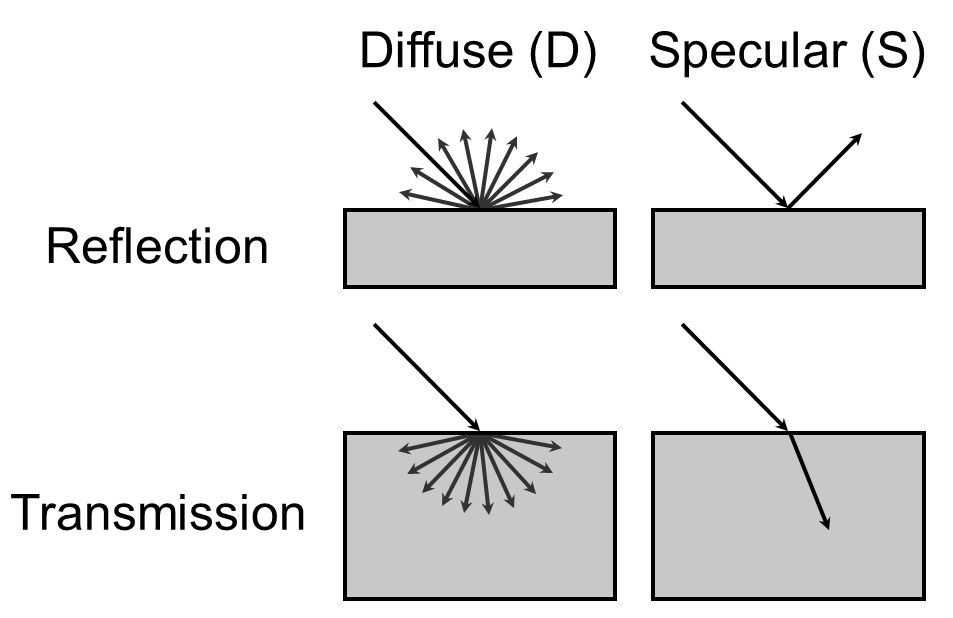
\includegraphics[width=0.5\textwidth]{./Chapter1/nanoscale2.png}
\caption[Comparison of specular and diffusive scattering processes.]{Comparison of specular and diffusive reflection and transmission. In general, specular scattering occurs from interfaces which are "smooth" with respect to the incoming wave, and the reflected/transmitted waves will retain memory of their momenta prior to scattering. Diffuse scattering occurs from "rough" interfaces, causing completely random scattering with no dependence on the history of the incoming wave.}
\label{f:ch1nano2}
\end{center}
\end{figure}

\subsubsection{The Acoustic Mismatch Model} In the AMM, phonons propagating towards an interface are assumed to interact with that interface as a sharp discontinuity of acoustic impedance, $Z_i$, where:
\begin{equation}\label{eq:nanoheat10}
Z_i = \rho_ic_i
\end{equation}
In the above equation, $\rho_i$ is the mass density of medium $i$ and $c_i$ is the acoustic velocity. Phonons may be reflected by the interface or refracted on the other side of it by following an equivalent of Snell's Law, given by Equation \ref{eq:nanoheat11}:
\begin{equation}\label{eq:nanoheat11}
\frac{\sin{\theta_1}}{c_1} = \frac{\sin{\theta_2}}{c_2}
\end{equation}
In Eq. \ref{eq:nanoheat11}, $\theta_1$ and $\theta_2$ are the incident and refraction angles, respectively. Several assumptions are implicit in utilizing Snell's Law here. Firstly, it is also assumed that phonon polarization is conserved. Secondly, the AMM as presented here assumes that interfacial scattering is elastic; that is, phonons conserve their frequency. As a consequence, phonons having a frequency above the Debye frequency of the softer (that is, having a lower Debye frequency) material are confined in the harder (that is, having a higher Debye frequency) material and do not cross the interface ($\alpha \rightarrow 0$). For phonons with frequencies smaller than the Debye frequency of the softer material, the transmission coefficient is derived from Snell's Law:
\begin{equation}\label{eq:nanoheat12}
\alpha_{1 \rightarrow 2}  = \frac{4Z_1Z_2\mu_1\mu_2}{\left(Z_1\mu_1 + Z_2\mu_2\right)^2} 
\end{equation}
In Eq. \ref{eq:nanoheat12}, $\mu_i = \cos{\theta_i}$. The derivation of Eq. \ref{eq:nanoheat12} from Snell's Law is straightforward, albeit lengthy, and was originally published by Little \cite{little1959transport}, to whose work the reader is referred for the full derivation.  
\subsubsection{The Diffuse Mismatch Model}
When phonon wavelengths are comparable to or smaller than interfacial roughness, phonons scattering at the interface are assumed to lose all information about the medium from which they originated. Thus, the probability of phonon transmission from medium 1 to 2 is equal to the probability that a phonon experiences a reflection in medium 2, i.e.
\begin{equation}\label{eq:nanoheat13}
\alpha_{1 \rightarrow 2} = 1 - \alpha_{2 \rightarrow 1}
\end{equation}
Following the derivation of Swartz and Pohl \cite{RevModPhys.61.605} we arrive at the DMM expression for the transmission coefficient:
\begin{equation}\label{eq:nanoheat13}
\alpha_{1 \rightarrow 2} = \frac{c_2g_2\left(\omega\right)}{c_1g_1\left(\omega\right) + c_2g_2\left(\omega\right)}
\end{equation}
In Eq. \ref{eq:nanoheat13}, $g_i\left(\omega\right)$ is the phonon density of states in medium $i$. Note that the DMM also assumes that high-frequency phonons are in confined the harder material \cite{PhysRevB.86.094303}. 
\subsubsection{Approximations for Phonon Lifetime}
The simplest approximation for the phonon lifetime, originally proposed by Callaway \cite{PhysRev.113.1046}, is the assumption that Umklapp scattering processes dominate the phonon relaxation. Umklapp scattering is a type of phonon-phonon scattering wherein scattered phonons exhibit a wavevector exceeding the boundary of the first Brillouin zone. This necessarily alters the direction of flux for scattered phonons and is partly responsible for the diffusive nature of phonon transport in bulk materials. Within the Callaway model, phonon lifetimes have the following dependence:
\begin{equation}\label{eq:nanoheat13}
\tau_i(\omega) = A_i\omega^{-2}
\end{equation}
In Equation \ref{eq:nanoheat13}, $A_i$ is collection of material-specific, temperature dependent parameters \cite{PhysRevB.86.094303}, and $\omega$ is the phonon frequency. While this approximation can work well for bulk materials and isolated crystalline interfaces, attempts to apply this model to nanostructured systems yield significant deviation of experimental results from the theory at elevated temperatures \cite{liu2006thermal}. Considering the dominance of interfacial phenomena at the nanometer length scale, the Callaway model is unlikely to suitably model phonon lifetimes for the systems studied in this thesis. 
\subsubsection{Application to Chemically-passivated, Nanometer-scale Systems}
The assumptions inherent in the models described above make them difficult to apply directly to the systems of interest here, which typically present chemically-passivated (usually by long-chain organic molecules such as alkylamines, alkanethiols, and organophosphorous species) interfaces on nanometer length scales. In particular, both the AMM and DMM require knowledge of the material sound velocity, which is typically poorly characterized for organic monolayers. Furthermore, at ambient temperatures, Umklapp scattering processes do not necessarily determine phonon relaxation times. While more advanced models of phonon lifetime exist based on anharmonic lattice dynamics \cite{PhysRevB.80.165304}, the effects of nanoscale confinement and atomic-scale disorder (introduced by the chemical passivating layer) on these models is generally unknown. Thus, we focus our theoretical efforts on molecular dynamics simulations, which make no assumptions regarding the nature of phonon scattering and can account for chemical details in a fully atomistic way. We elaborate on some of these considerations in Chapter 3.
\section{Outline}
The work in this thesis is divided into two major categories: Thermal processes in semiconductor nanocrystals and photoluminescence (PL) in group-IV semiconductor nanocrystals. In Chapter 2, we review the experimental details of ultrafast optical spectroscopy, necessary to characterize the carrier dynamics exhibited by these materials in real time. Next, we explore the earliest stages of heat generation - energy dissipation by photoexcited charge carriers. We apply a recently developed technique, femtosecond stimulated Raman spectroscopy, to directly observe, for the first time, phonon generation as a result of carrier cooling in CdSe nanocrystals. We find a lack of size-dependence in phonon generation dynamics, consistent with size-independent hole-phonon coupling in these materials. In addition to laying the groundwork for more advanced studies of vibrational energy flow in NC systems, these results lend credence to as-yet unproven theories regarding confinement enhanced, Auger-like electron-to-hole energy transfer in II-VI semiconductor nanocrystal compositions. \par
In Chapter 3, we focus on the fate of phonons after they are generated. First, we characterize a previously-unexplained ultrafast decay feature evident in the low-temperature PL dynamics of matrix-embedded CdSe nanocrystals. Utilizing streak camera measurements and a size-series of CdSe NCs, we are able to attribute this decay feature to rapid emission facilitated by non-equilibrium acoustic phonons generated by carrier cooling. We further associate the decay of this PL feature with acoustic phonon outflow and demonstrate that this optical signature can be used to characterize thermal transport rates at the NC-matrix interface. Next, we examine the interfacial thermal transport process for chemically-passivated NCs with atomistic resolution using molecular dynamics (MD) simulations. Specifically, we utilize a recently-developed MD method well-suited to the study of transport at heterogeneous, acoustically mismatched interfaces. We demonstrate that thermal transport at the semiconductor/solvent interface is significantly enhanced by the presence of surface ligands and that the underlying structure of the exposed semiconductor surface places fundamental limits on thermal conductance because it controls maximal ligand grafting density. \par
In Chapter 4, several chemical methods for manipulating thermal processes in NCs are explored. Primarily, we utilize the optical signature of thermal transport detailed in Chapter 3 to characterize a range of NCs presenting a fixed core size with increasingly thick, optoelectronically inert shells. We demonstrate that inert shell growth permits separate tuning of the thermal and optical properties of NCs. We also briefly report on theoretical work done in support of larger experimental efforts. Specifically, we discuss the possibility that two new surface termination motifs (passivation by small, inorganic capping ligands and covalently-bound ligands) may confer thermal stability benefits similar to those provided by shell growth, but without confining one or both charge carriers to the NC core (which hinders their application in technologies requiring carrier mobility). \par
Chapter 5 contains the second major category in this thesis. We report a detailed experimental and theoretical investigation of PL enhancement in silicon nanocrystals. Radiative recombination becomes efficient in nanometer-scale silicon materials, but the mechanism of enhanced photon emission has long been contested, with a variety of mechanisms each having a substantial body of supporting literature. In particular, efficient PL from silicon NCs has been attributed to relaxation of momentum-conservation requirements by translational symmetry loss, emission from surface oxide species, direct-gap emission from hot carriers, and quasidirect emission from band-edge states broadened in $k$-space by ligand species. We utilize pressure-dependent optical spectroscopy and find that the pressure-induced shift of steady-state PL from silicon NCs matches the band-edge pressure coefficient of bulk Si. Combined quantum/classical simulations of silicon NCs under pressure yield a similar dependence of the NC energy gap and further confirm that the band-edge states are delocalized throughout the NC rather than confined to a surface state. Taken together, these results strongly suggest that band-edge PL in silicon NCs remains indirect in character despite substantial quantum confinement. Next, we explore high-energy, short-lived PL using time-resolved PL spectroscopy and Raman spectroscopy. We investigate PL dynamics as a function of NC size and lattice crystallinity and, in conjunction with molecular dynamics simulations and TEM characterization, attribute high-energy PL to an emissive amorphous surface layer. \par
Finally, in Chapter 6, we present structural characterization of group-IV nanocrystals at elevated pressures. While the main focus of our pressure-dependent work was on elucidating the origin of light emission in these materials, the pressure-dependent structural properties of NCs are interesting enough to merit some separate discussion. We present pressure-dependent XRD of both silicon and Ge nanocrystals. Interestingly, we find these particles to exhibit compressibility matching the bulk phase, in contrast to most other NC compositions. We also analyze molecular dynamics simulations of the pressurization process to provide insight regarding the nature of pressure-induced structural changes in these materials.
\chapter{Initital Stages of Heat Generation: Electron-phonon Thermalization in Nanoscale Systems}	% Chapter 2.

Work presented in this chapter is adapted from the following paper:

\begin{itemize}
\item Hannah, D. C.; Brown, K. E.; Young, R. M.; Wasielewski, M. R.; Schatz, G. C.; Co, D. T.; Schaller, R. D. \emph{Phys. Rev. Lett.} \textbf{2013}, 111, 107401
\end{itemize}

Theoretical work in this chapter is adapted, in part, from the following paper:

\begin{itemize}
\item Aruda, K. O.; Tagliazucchi, M.; Sweeney, C. M.; Hannah, D. C.; Schatz, G. C.; Weiss, E. A. \emph{Proceedings of the National Academy of Sciences} \textbf{2013}, 110, 4212–4217.
\end{itemize}

\section{Overview}

Subsequent to the excitation of charge carriers, often by an applied electromagnetic field, excited electrons and holes dissipate energy by thermalizing with vibrational degrees of freedom in the host lattice as well as the surrounding environment (such as ligand and solvent/matrix vibrations). Such thermalization processes are a key energy loss mechanism in semiconductor materials and a contributor to heat generation, so controlling these processes is of technological interest. While carrier thermalization has been studied extensively in bulk materials and for over a decade in nanomaterials, several open questions remain. As discussed in Chapter 1, the absence of a theoretically predicted phonon bottleneck in strongly-confined semiconductor NCs has stimulated a body of work attempting to resolve the true nature of carrier energy loss mechanisms in these materials. The prevailing interpretation of carrier thermalization invokes Auger-like energy transfer between the electron and hole (as discussed in Chapter 1). However, Auger-like energy transfer remains unproven, and several recent experimental results call this explanation into question. For example, removal of the hole (which nominally receives energy from the electron, facilitating electron cooling) does not significantly slow electron cooling rates \cite{PhysRevB.60.R2181, klimov2000mechanisms}. Furthermore, materials exhibiting similar carrier effective masses, such as PbSe, also exhibit subpicosecond carrier cooling despite the expectation that Auger-like energy transfer should not productively yield carrier cooling in such materials \cite{wehrenberg2002interband, harbold2005time}. These results would seem to suggest that multi-phonon transitions somehow become significantly more efficient or that higher-energy ligand vibrations are able to participate in the carrier thermalization process. \par

Direct examinations of phonon generation during NC carrier cooling remain missing from the literature, despite the evident importance of this process to understanding carrier energy loss in NCs. In this Chapter, we first detail the experimental setups and methods used to characterize ultrafast processes in NCs throughout this thesis. \par

Next, we report femtosecond stimulated Raman spectroscpoy measurements of lattice dynamics in semiconductor nanocrystals and characterize longitudinal optical (LO) phonon production during confinement-enhanced, ultrafast intraband relaxation. Stimulated Raman signals from unexcited CdSe nanocrystals produce a spectral shape similar to spontaneous Raman signals. Upon photoexcitation, stimulated Raman amplitude decreases owing to experimentally resolved ultrafast phonon generation rates within the latice. We find a $\sim$600 fs, particle-size-independent depletion time attributed to hole cooling, evidence of LO-to-acoustic down-conversion, and LO phonon mode softening. \par

Finally we briefly consider the role played by surface ligands in mediating analogous processes (hot electron cooling) in similarly-sized metallic nanoparticles. Specifically, we report density functional theory (DFT)-derived electronic structure calculations on thiol- and amine-passivated gold slabs. We find that thiol-functionalization greatly increases the density of electronic states near the gold Fermi level as compared to the aminated case, resulting in elevated electronic heat capacity. This elevated electronic heat capacity manifests as a longer hot electron lifetime, which is observed using transient absorption spectroscopy.

\section{Experimental Characterization of Carrier Cooling in Semiconductor Nanocrystals}

As discussed in the introductory Chapter of this thesis, intraband relaxation in NCs generally proceeds on a sub-picosecond timescale. Therefore characterization of the carrier cooling process is typically accomplished using time-resolved optical spectroscopy, which is capable of providing the extremely high time-resolution required. The work presented in this Chapter makes use of two spectroscopic pump-probe techniques sensitive to dynamics on these timescales: Transient absorption spectroscopy (TA) and femtosecond stimulated Raman spectroscopy (FSRS). We briefly review each technique and the experimental setups we utilized here.

\subsection{Transient Absorption Spectroscopy}
\subsubsection{Overview}
In transient absorption spectroscopy, two ultrashort pulses ($< 50$ fs) are used to study the dynamic evolution of a sample absorption spectrum. The first pulse, termed the pump pulse, initiates a time-dependent process in the sample. A mechanically delayed second pulse, termed the probe pulse, interrogates the sample absorption spectrum at various times subsequent to photoexcitation. The nature of these pulses can vary according to experimental needs; we will review our setup in the next section. The transient absorption spectrum is calculated according to Equation \ref{eq:ta1}:
\begin{equation}\label{eq:ta1}
\Delta OD(\lambda, t) = OD(\lambda, t)_{ON} - OD(\lambda, t)_{OFF} = \log{\frac{I(\lambda, t)_{OFF}}{I(\lambda,t)_{ON}}}
\end{equation}
"ON" and "OFF" refer to probe spectra collected with and without the pump pulse.  These spectra are generally obtained by mechanically chopping the pump pulse.
\subsubsection{Experimental TA apparatus}

\begin{figure}
\begin{center}
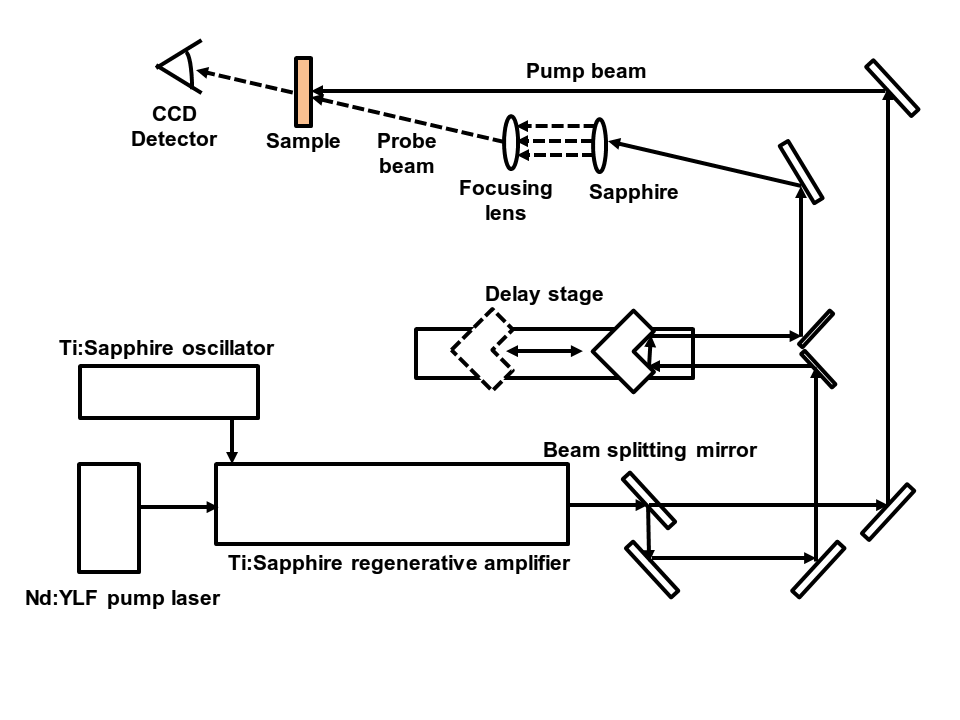
\includegraphics[width=\textwidth]{./Chapter2/ta_setup.png}
\caption[Block diagram of transient absorption apparatus.]{Block diagram of the experimental appartus used to collect the transient absorption and time-resolved PL data presented in this work.}
\label{f:tasetup}
\end{center}
\end{figure}

Unless otherwise noted, the transient absorption measurements described in this work were carried using the apparatus depicted in Figure \ref{f:tasetup}. A regeneratively amplified Ti:Sapphire laser operating at a 2-kHz repitition rate was used to generate 35 fs pulses with a wavelength of 800 nm. A portion (5\%) of the amplifier output was time-delayed and focused onto a sapphire plate to produce a white-light probe pulse. The remaining output was either frequency-doubled to 400 nm or used to feed an optical parametric amplifier (OPA) for spectrally tunable pump pulses. Pump and probe pulses were overlapped on the sample, and pump pulses were mechanically chopped at a frequency of 1 kHz.

\subsubsection{Special Considerations for Nanocrystals}
One of the most important features of the transient absorption spectrum of CdSe nanocrystals is the $1S_{3/2}-1S_e$ bleach, corresponding to the band-edge exciton. In nanocrystals, state filling leads to bleaching of the interband transitions between populated quantized states \cite{doi:10.1021/jp9944132}. \par

The valence band in CdSe nanocrystals is 3-fold degenerate. Additionally, the hole in this material exhibits a much larger effective mass than the electron such that $m_h/m_e \approx 6$. Because of this, the thermal occupation probabilities of electron states are far greater than those of the coupled hole states. Put simply, the thermal distribution of hole populations is spread over many levels. A consequence of this asymmetry between electron and hole populations is that the $1S_{3/2}-1S_e$ bleach feature in TA spectra is sensitive primarily to electron populations \cite{doi:10.1021/jp9944132}. 

\subsection{Femtosecond Stimulated Raman Spectroscopy}
\subsubsection{Overview}
Similar to transient absorption spectroscopy, the femtosecond stimulated Raman spectroscopy (FSRS) process begins with an ultrashort laser pulse, termed here the actinic pulse, which initiates a time-dependent process in the sample of interest. The evolution of the structure and vibrational populations of the system are interrogated after a time delay by a pair of pulses which drive stimulated Raman transitions in the sample: a narrow bandwidth, temporally broad Raman pulse and short broadband probe pulse. When these two pulses are simultaneously incident on the sample, Raman transitions having a frequency of $\omega_v = \omega_{Probe} - \omega_{Raman}$ cause a net attenuation of the pump beam and net gain in the probe beam. The final Raman scattering spectrum is obtained by dividing out a probe spectrum without a co-incident Raman pump pulse, similar to the pump-off/pump-on motif shown in Eq. \ref{eq:ta1}, but with the Raman pulse being mechanically chopped \cite{doi:10.1146/annurev.physchem.58.032806.104456}. \par

The time resolution of FSRS is determined only by the duration of the actinic and Raman pump pulses. The detection of FSRS is not time-resolved, and so the frequency resolution of FSRS is independent of the time-energy Fourier limitations of the femtosecond pulses. Thus, FSRS is one of the only techniques capable of probing the dynamics of low-frequency vibrations on sub-picosecond timescales. This makes it ideally suited to the examination of the role played by (low-frequency) phonons in NC intraband carrier cooling.

\subsubsection{Experimental FSRS Apparatus}

\begin{figure}
\begin{center}
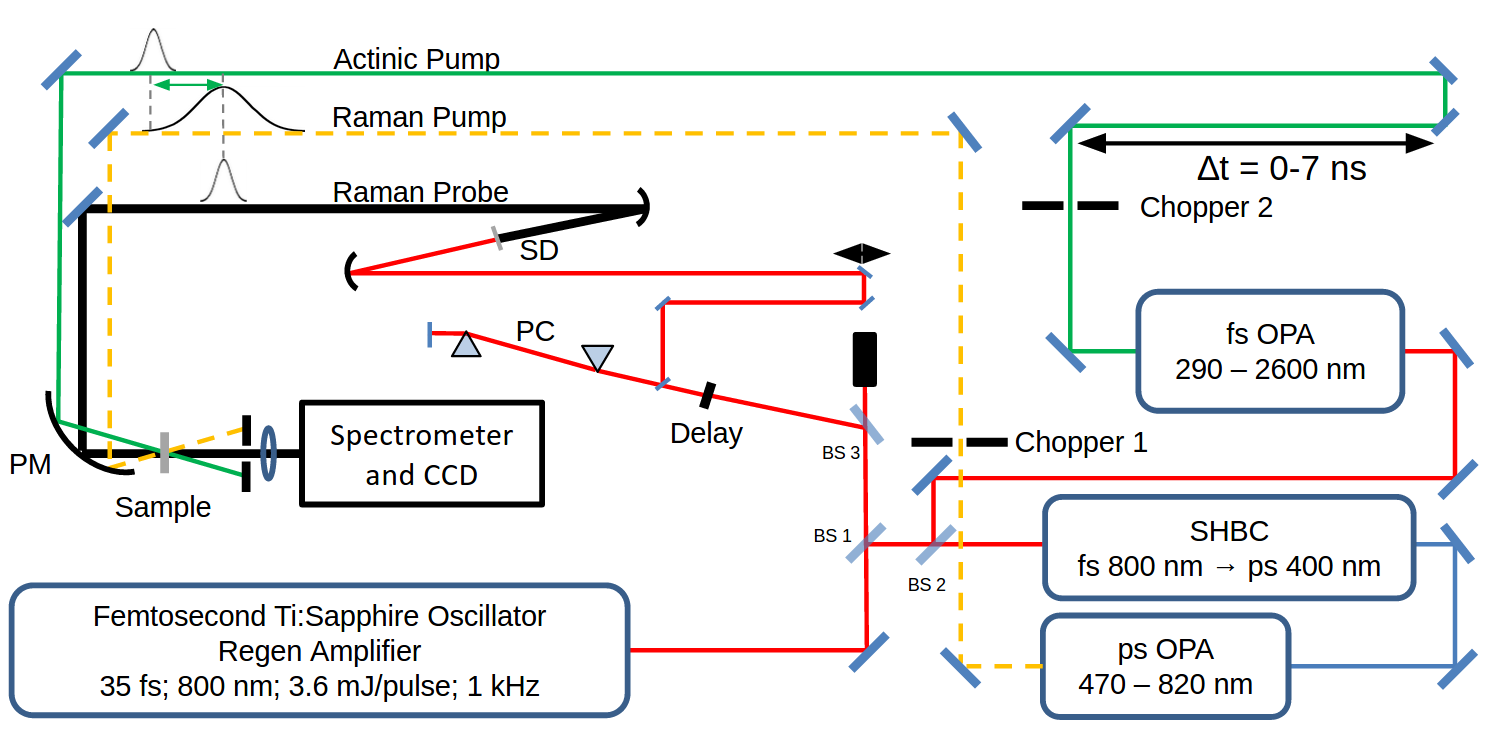
\includegraphics[width=\textwidth]{./Chapter2/fsrs_setup.png}
\caption[Block diagram of femtosecond stimulated Raman spectroscopy apparatus.]{Block diagram of the experimental apparatus \cite{doi:10.1021/jz301107c} used to collect the femtosecond stimulated Raman spectroscopy data presented in this Chapter.  Reproduced from Ref. 15.}
\label{f:fsrssetup}
\end{center}
\end{figure}

Figure \ref{f:fsrssetup} displays the experimental setup utilized here for the acquisition of FSRS data. The 800 nm, 35-fs pulse output of regeneratively amplified Ti:Sapphire laser operating at 1 kHz is split first using a 80\% reflective beamsplitter (BS1 in Fig. \ref{f:fsrssetup}). The transmitted portion is is directed to a second beamsplitter (BS3), which transmits 10\% of the remaining output to a sapphire disk in order to produce the white light probe pulse. The reflected portion of the initial amplifier output is sent through a 50\% beam splitter (BS2). The transmitted portion is frequency doubled with a second harmonic bandwidth compressor (SHBC) to give a 400-nm pulse. This pulse is used to seed a narrow bandwidth ps-OPA, which provides a spectrally tunable Raman pulse. The reflected portion is directed to a second, femtosecond OPA to produce short, spectrally tunable actinic pump pulses. Time delay between the actinic pump and Raman/probe pulse pair is controlled \emph{via} a motorized delay stage in the actinic pump beam path. The Raman pulse is chopped at a frequency of 125 kHz to obtain pump on and pump off spectra. The full details of this setup are reported in work by Brown \emph{et al.} \cite{doi:10.1021/jz301107c}

\section{Basic Characterization of CdSe Nanocrystals}
The CdSe nanocrystals utilized in the experiments reported in this Chapter (as well as Chapter 3) were examined by absorption spectroscopy as well as transmission electron microscopy in order to characterize particle size and shape. Figure \ref{f:basic1} displays the static UV-visible absorption spectrum of various CdSe NC sizes suspended in hexane. The spectra exhibit (expected) features characteristic of quantum confinement, including a sharp excitonic peak and size-dependent absorption onsets. 

\begin{figure}
\begin{center}
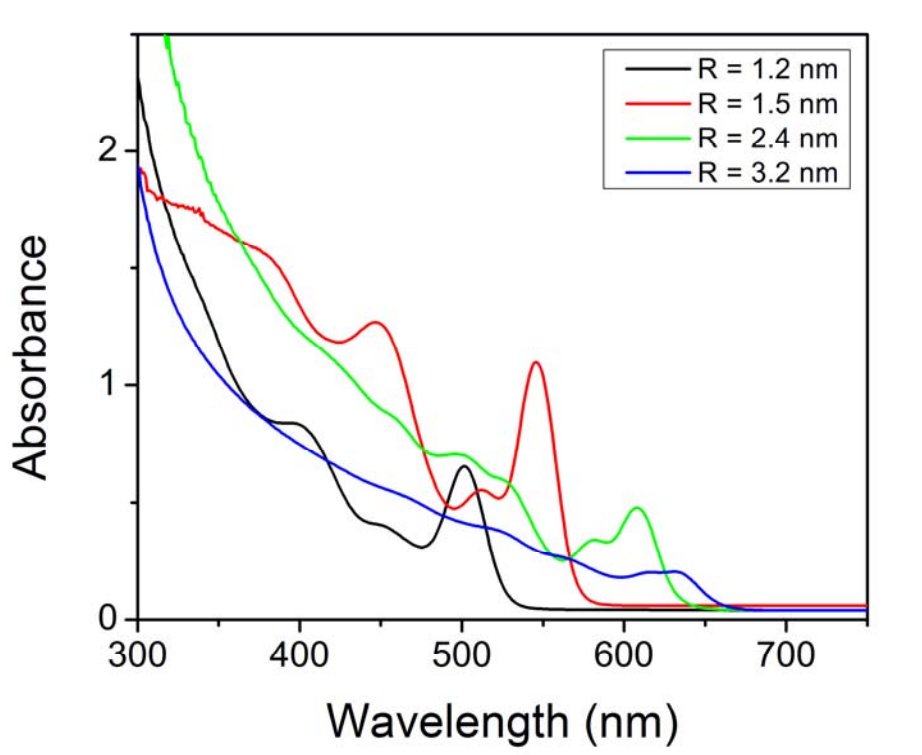
\includegraphics[width=0.75\textwidth]{./Chapter2/basic1.png}
\caption[Absorption spectra of CdSe NC samples examined in this work.]{UV-visible absorption spectra of four sizes of CdSe NC suspended in hexane.  Average particle radii are indicated in the figure legend.}
\label{f:basic1}
\end{center}
\end{figure}

Figure \ref{f:basic2} shows a transmission electron micrograph of CdSe collected on an amorphous carbon substrate. These particles are spherical in shape an exhibit the wurtzite crystal structure.

\begin{figure}
\begin{center}
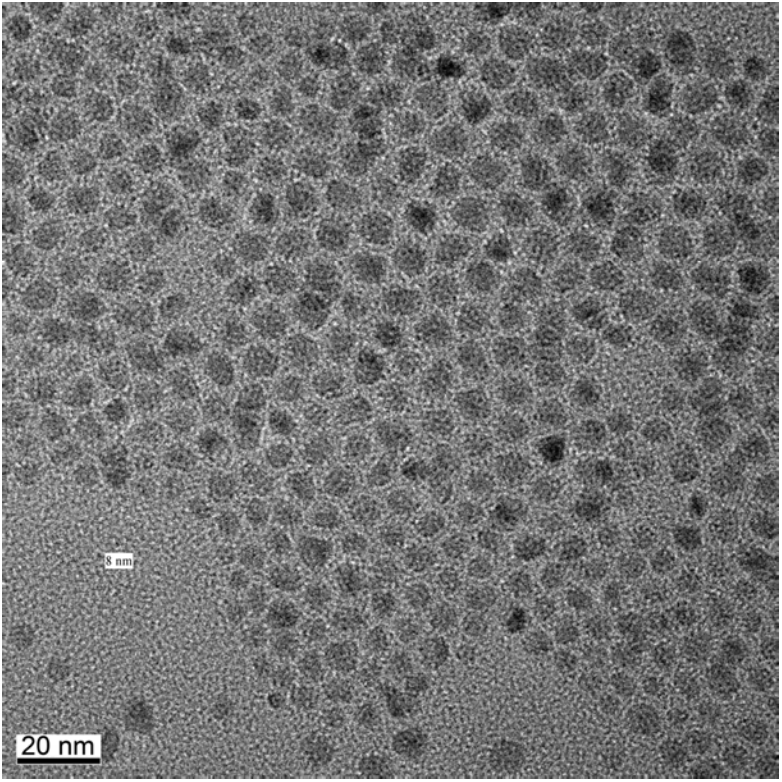
\includegraphics[width=0.75\textwidth]{./Chapter2/basic2.png}
\caption[Transmission electron micrograph of CdSe NCs.]{Transmission electron micrograph of CdSe nanocrystals.}
\label{f:basic2}
\end{center}
\end{figure}


\section{Direct Characterization of Lattice dynamics in Semiconductor Nanocrystals Using FSRS}

As noted above, confinement-enhanced electron-to-hole Auger energy transfer has been suggested as the primary means of hot exciton cooling in CdSe NCs where electron excess energy is transferred to holes that then rapidly cool via phonon emission \cite{Efros1995281}.  Experimentally, transient absorption (TA) measurements show faster intraband exciton cooling in smaller particles with larger bandgaps \cite{PhysRevB.60.13740, PhysRevB.60.R2181, PhysRevLett.80.4028}, consistent with the proposed mechanism. Since bleach signals in CdSe NCs predominantly arise from excited electrons, these measurements specifically convey NC size-dependent electron cooling rates \cite{Wang23032001, doi:10.1021/ja070099a, doi:10.1021/jp9944132}.  Recently, Xu \emph{et al.} observed rapid hole cooling times via comparison of TA and femtosecond up-conversion measurements \cite{PhysRevB.65.045319}.  Similarly, Hendry et al. measured the non-resonant transient conductivity of photo-excited NCs using terahertz time-domain spectroscopy and reported a $\sim$1 ps electron-hole coupling time \cite{PhysRevLett.96.057408}.  Missing from the literature are direct examinations of lattice dynamics during this process. Such measurements present inherent challenges as the typical sub-picosecond carrier relaxation lifetimes and small phonon energies obviate the utility of transient spontaneous Raman spectroscopy \cite{PhysRevB.80.121403}.  \par

We utilized FSRS, notable for the high temporal ($\sim$100 fs) and energy ($\sim$10 cm$^{-1}$) resolution described above \cite{doi:10.1146/annurev.physchem.58.032806.104456}, to investigate phonon dynamics in photoexcited NCs for the first time.  For CdSe NCs, we observe sub-picosecond phonon dynamics along with mode softening, and note a lack of size dependence for the initial change in signal levels despite size-dependent electronic intraband relaxation \cite{Wang23032001, doi:10.1021/ja070099a, doi:10.1021/jp9944132}.  We attribute the initial FSRS depletion time constant to size-independent hot-hole-to-phonon coupling. We also observe a rapid ($\tau$ = $\sim$2 ps) recovery of the stimulated Raman signal that is consistent with relaxation of LO phonon populations into other vibrational modes.  This rapid phonon downconversion is followed by a slower recovery of gain amplitude with a timescale and size-dependence consistent with phonon outflow from the NC into the surrounding matrix. Diminished gain amplitude at even longer times ($\sim$1 ns) is suggestive of persistent LO-phonon generating processes or altered phonon coupling in NCs containing a band-edge exciton, for which the radiative lifetime is on the order of nanoseconds. \par

We examine hexane suspensions of octadecylamine-capped CdSe NCs with spherical particle shapes, and optical properties as noted in Qu \emph{et al.} \cite{doi:10.1021/ja017002j}.  Figure \ref{f:fsrs1} shows a schematic depicting the FSRS experiment in the context of NC dynamics.  The details of the experimental setup are reported above and elsewhere \cite{doi:10.1021/jz301107c}.  Here, we adjust the actinic and Raman pump fluences such that the average number of electron-hole pairs generated per NC is less than 0.2 \cite{doi:10.1021/jp9944132}.  This assures that dynamics related to single excitons are observed. Optical Kerr-effect (OKE) cross-correlation of the actinic pump and probe pulses in hexane indicates a time resolution of $\sim$170 fs. \par

\begin{figure}
\begin{center}
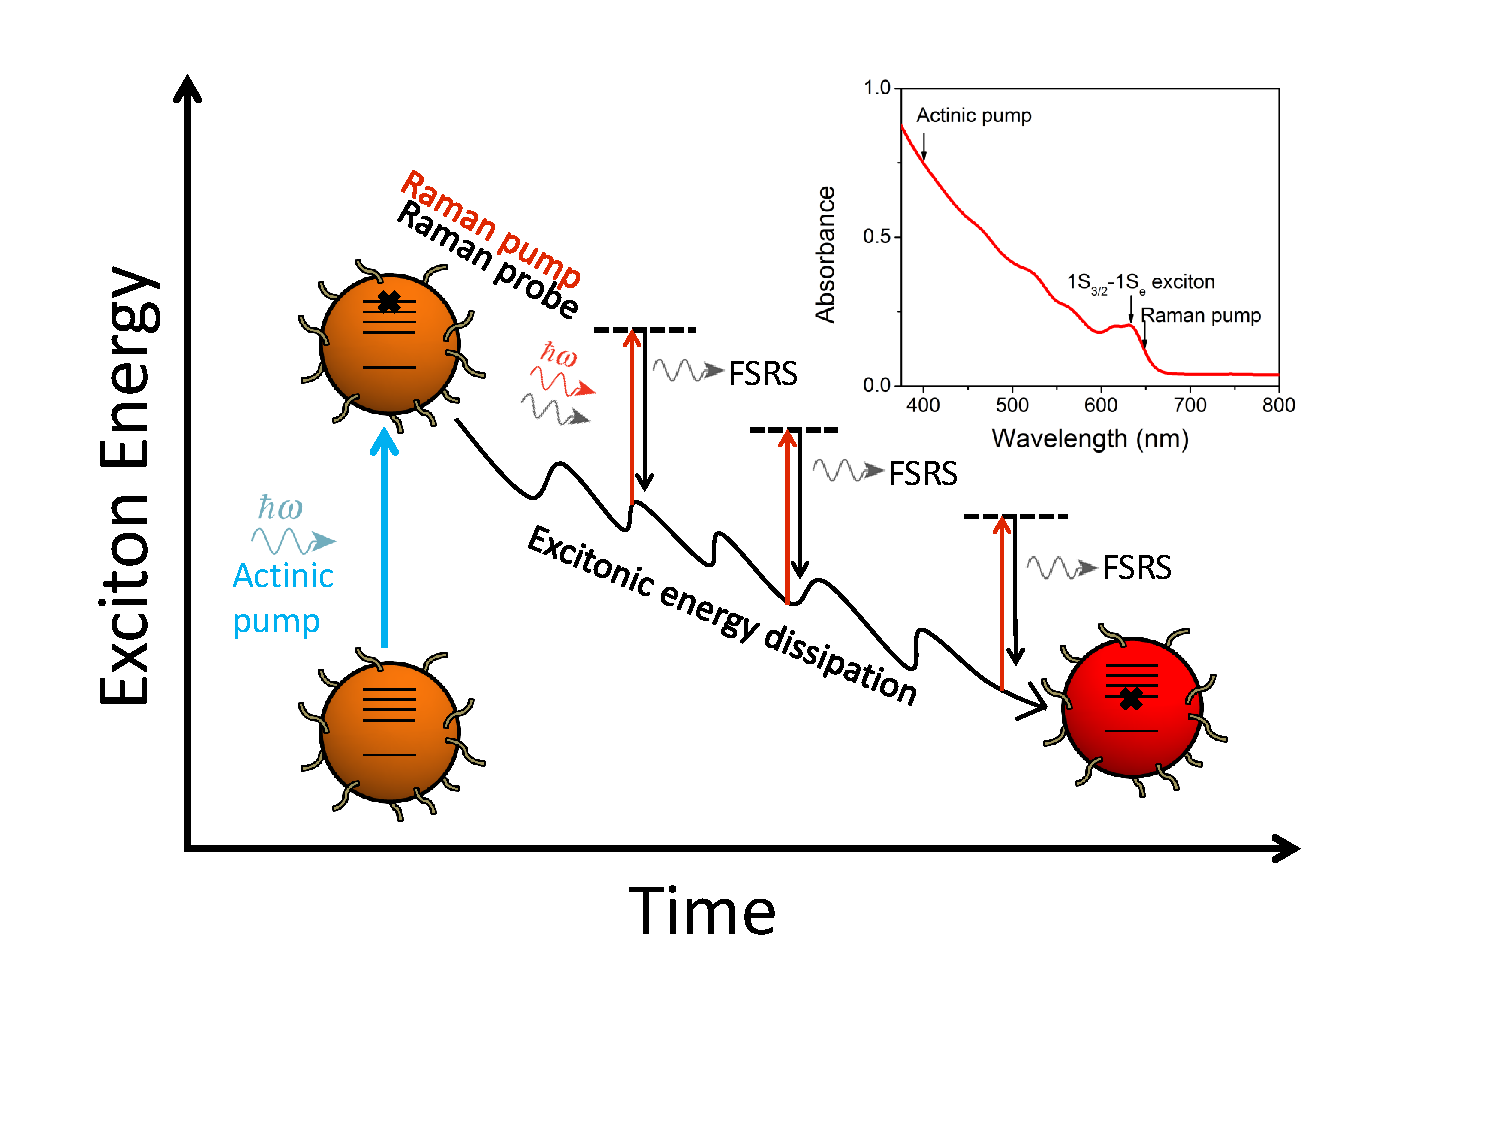
\includegraphics[width=\textwidth]{./Chapter2/fsrs1.pdf}
\caption[Diagram demonstrating the application of FSRS to exciton cooling in NCs.]{An actinic pump photon, having energy greater than the NC energy gap, excites a hot electron-hole pair, denoted by ‘X’.  The ladder levels represent exciton (\emph{i.e.} electron + hole) states.  As the system evolves in time, hot carriers cool via various pathways including phonon emission and Auger-like electron-to-hole energy transfer.  The Raman pump, which is resonant with electronic transitions in the NC, and probe pulses stimulate Raman transitions at various time delays, generating FSRS signal. Inset: Absorption spectrum of 3.1-nm radius CdSe nanocrystals capped with octadecylamine and suspended in hexane.  The actinic pump and Raman pump wavelengths are indicated relative to the 1S$_{3/2}$-1S$_e$ exciton transition.}
\label{f:fsrs1}
\end{center}
\end{figure}

Figure \ref{f:fsrs2}(a) displays raw FSRS spectra of colloidal CdSe NCs with a 1.5 nm radius. The features observed are consistent with previous static measurements of resonant Raman scattering in this material \cite{aliviresodepolar}.  The peak at $\pm$210 cm$^{-1}$ corresponds to the longitudinal optical (LO) phonon mode of the CdSe lattice and a 2LO phonon Raman peak also appears at $\pm$410 cm$^{-1}$.  Atypically, the CdSe phonon features exhibit gain at both Stokes and anti-Stokes frequencies.  A low-frequency shoulder on the LO phonon feature, commonly observed in spontaneous Raman and attributed to the surface optical (SO) phonon mode \cite{aliviresodepolar, DzhaganPhonon} is reproducibly observed both here (Fig. \ref{f:fsrs2}(a), inset) as well as in static Raman spectra.  To analyze each mode, we fit the LO phonon feature using the sum of two Gaussians as illustrated in the inset of Fig. 2(a). In the dynamics experiments discussed later in this report, we note that the LO and SO phonon modes exhibit indistinguishable dynamics, suggestive of a single population exhibiting both phonon features. \par

\begin{figure}
\begin{center}
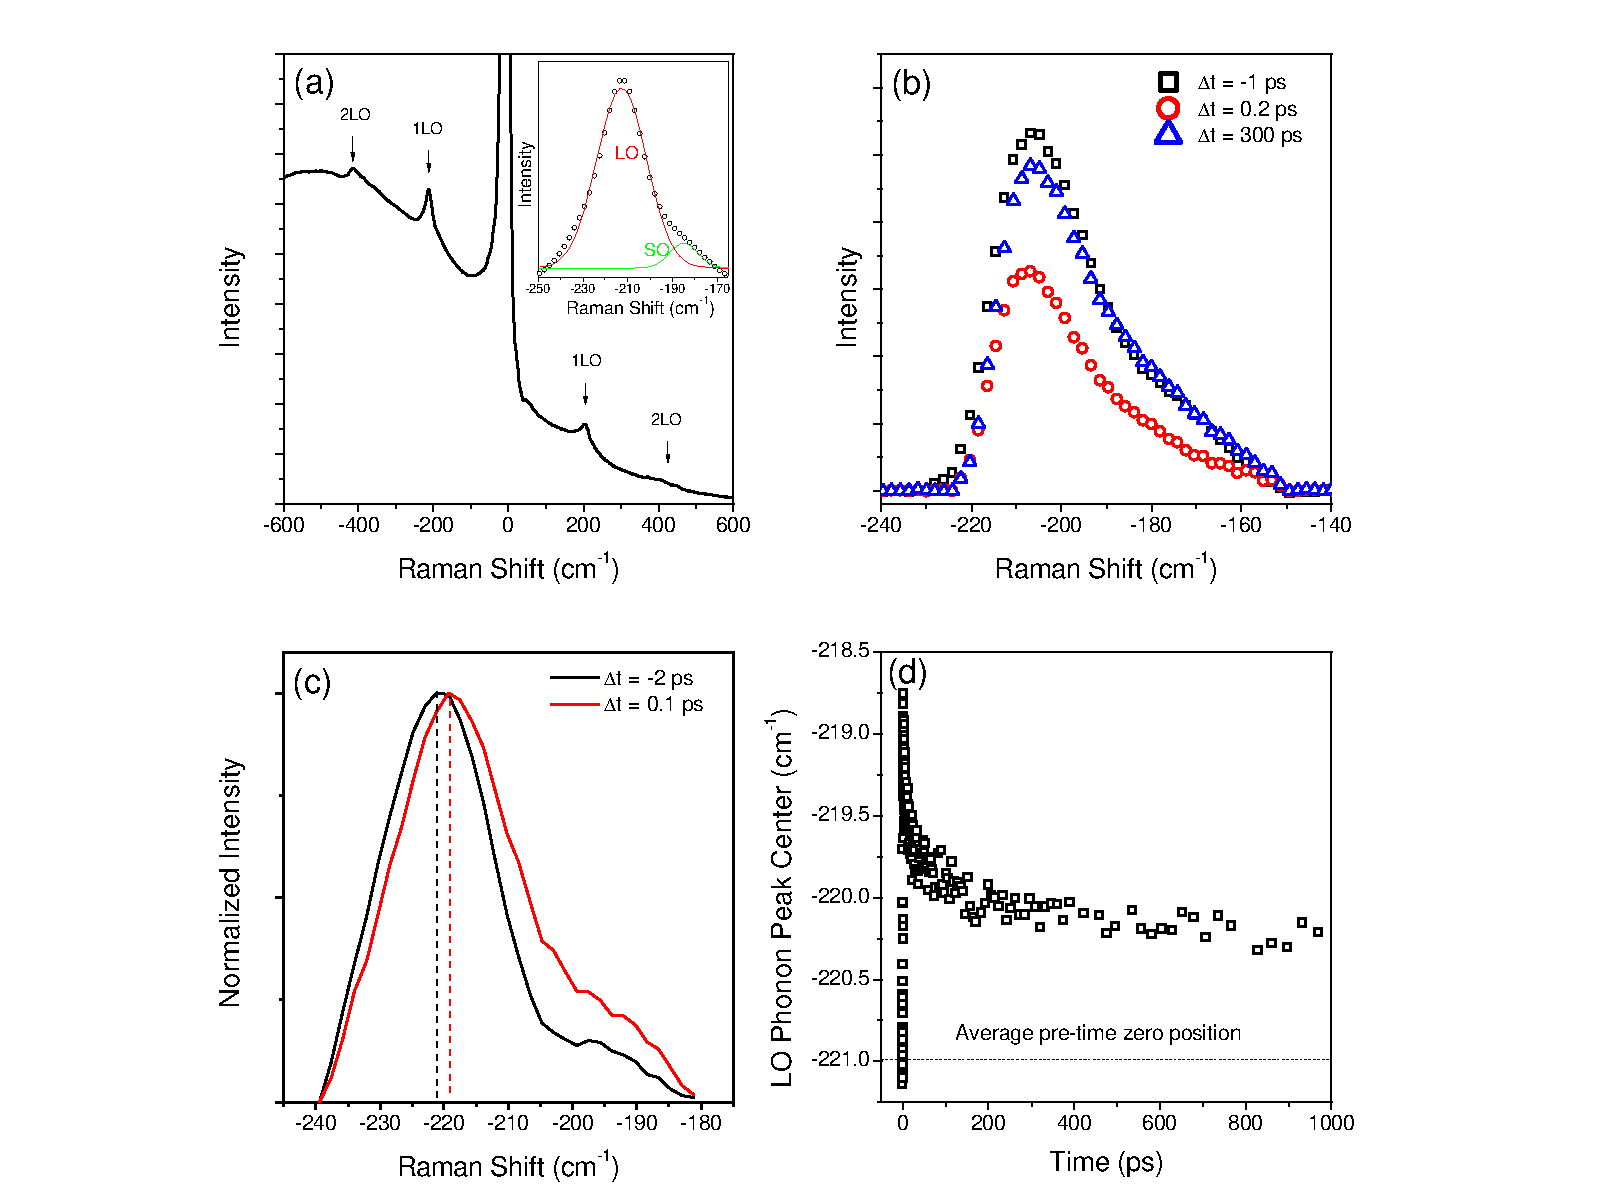
\includegraphics[width=\textwidth]{./Chapter2/fsrs2.pdf}
\caption[Features of FSRS spectra of CdSe NCs.]{(a) Raw ground-state FSRS spectrum for 3.1 nm radius CdSe NCs suspended in hexanes at negative time delay (prior to photoexcitation by the actinic pump). 1LO and 2LO phonon features are indicated. The inset displays a fit of the background-subtracted anti-Stokes peak to the sum of two Gaussian functions. The blue line indicates the overall fit. In accordance with previous reports, the Gaussian function given in red is assigned to the LO phonon mode, while the blue Gaussian function is assigned to the SO phonon mode. (b) Background-subtracted anti-Stokes phonon peak for 3.1-nm radius CdSe NCs at indicated pump probe time-delays. (c) Normalized anti-Stokes phonon band for a 2.4-nm radius CdSe NC at the indicated time delays. The color-coded dotted line serves as a guide to the eye and represents the location of the LO phonon peak center as determined by fits of the phonon band to two Gaussian functions. (d) Dynamics of the LO phonon peak center for a 2.4-nm radius CdSe NC derived from the two-Gaussian fit. The location of the phonon peak center prior to photoexcitation is indicated by the dotted black line.}
\label{f:fsrs2}
\end{center}
\end{figure}

Figure \ref{f:fsrs2}(b) shows background-subtracted time-resolved spectra for the anti-Stokes 1LO phonon feature at three time delays relative to the 0.5 nJ/cm$^2$ actinic pump: Both the Stokes (not shown) and anti-Stokes gain amplitudes are depleted by photoexcitation, with partial recovery of the gain signal at longer times. Normalized, background-subtracted 1LO phonon FSRS spectra, presented in Fig. \ref{f:fsrs2}(c) for a 2.4 nm radius CdSe NC, prior to (-2 ps) and shortly after (0.1 ps) photoexcitation reveal that the 1LO phonon feature is red-shifted by approximately 2 cm$^{-1}$ for both the Stokes and anti-Stokes features. This redshift occurs upon generation of LO phonons by photoexcited NCs. The presence of excitons in NCs leads to a transient renormalization (softening) of the LO phonon frequency. To explain this, we consider the exciton-phonon interaction due to Frolich coupling. The general form of this interaction is shown in Equation \ref{eq:fsrs_eq1} \cite{PhysRevLett.80.3105}:
\begin{equation} \label{eq:fsrs_eq1}
H_{ex-LO} = \sum_{ij}\sum_{nlm}\gamma_{nlm}^{ij}c_i^{\dagger}c_j\left(a_{nlm}^{\dagger}+a_{nlm}\right)
\end{equation}
where $c_i$ denotes the annihilation operator for the $i$th exciton state $a_{nlm}$ is the phonon annihilation operator for the $n$th phonon having angular momentum $l$.  $\gamma_{nlm}^{ij}$ are the exciton-phonon coupling matrix elements.  In the case of strongly confined NCs (including CdSe), excitons couple strongly to LO phonons having $l = 0$ and their coupling can be expressed in terms of sine integrals \cite{1996JETP...83..610F}.  The form of the exciton-phonon matrix elements is given by Equation \ref{eq:fsrs_eq2}:
\begin{equation} \label{eq:fsrs_eq2}
\begin{split}
\gamma_{nlm}^{ij} =& -e\sqrt{\frac{\Omega}{\kappa R}}\left[\mathrm{Si}\left(\left(n+i-1\right)\pi\right) - \mathrm{Si}\left(\left(n+i+1\right)\pi\right)\right. \\
&+ \left.\mathrm{Si}\left(\left(n-i+1\right)\pi\right) - \mathrm{Si}\left(\left(n-i-1\right)\pi\right) \right]
\end{split}
\end{equation}
where, in this equation only, "Si" (not to be confused with silicon) denotes the sine integral, $\Omega$ is the Lo phonon frequency, and $\kappa = \frac{\epsilon_0\epsilon_\infty}{\epsilon_0 - \epsilon_\infty}$.  Once the coupling constants are obtained, the change in the phonon frequency for an excited NC may be calculated using second-order perturbation theory following the procedure described by Zimin \emph{et al.} \cite{PhysRevLett.80.3105}:
\begin{equation} \label{eq:fsrs_eq3}
\mathrm{d}\Omega = -\sum_{i \neq 0}\frac{|\gamma_n^{0i}|^2 2\left(E_i - E_0\right)}{\left(E_i - E_0\right) - \Omega^2}
\end{equation}
In Equation \ref{eq:fsrs_eq3}, $E_i$ denotes the energy of the $j$th exciton state.  Using Equations \ref{eq:fsrs_eq2} and \ref{eq:fsrs_eq3}, we carry out this analysis using CdSe material parameters.  For a 2.4-nm radius CdSe NC, we estimate a change in LO phonon frequency upon photoexcitation of -2.6 cm$^{-1}$, in good agreement with our observation.  Fig. \ref{f:fsrs2}(d) displays the dynamics of the LO phonon peak center for the same sample.  Following the initial red-shift, the 1LO phonon peak center shifts back towards its original position, but remains slightly red-shifted even at time delays of 1 ns, likely owing to a long-lived population of single excitons in photoexcited NCs. \par

\begin{figure}
\begin{center}
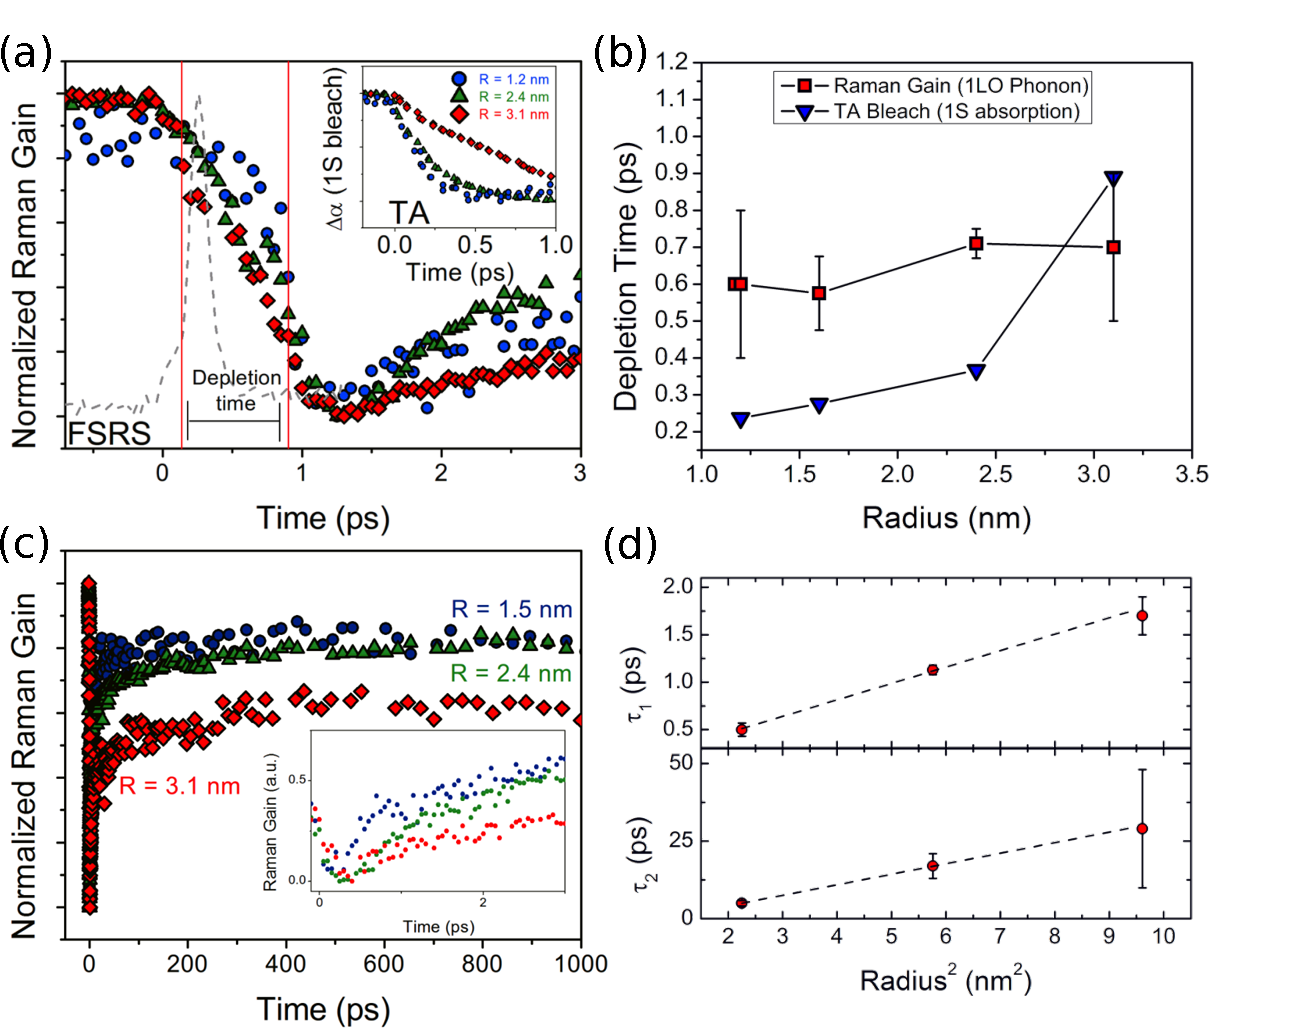
\includegraphics[width=\textwidth]{./Chapter2/fsrs3.pdf}
\caption[FSRS dynamics for a variety of CdSe NC sizes.]{(a) Anti-Stokes gain amplitude dynamics at the 1LO phonon frequency for CdSe NCs having radii of 1.2 nm (blue circles), 2.4 nm (green triangles), and 3.1 nm (red diamonds). Data are presented for time delays corresponding to the first few picoseconds
before and after the actinic pump arrival ($\Delta t = 0$).  The dotted gray line shows the IRF.  The vertical red lines indicate the signal depletion time, defined here as the time taken for the signal to drop from 80\% to 20\% of its initial ($\Delta t < 0$) intensity.  The inset displays transient absorption dynamics of the $1S_{3/2}-1S_e$ bleach feature for the same set of NCs.  (b) Anti-Stokes gain amplitude dynamics for 1.5 nm (navy circles), 2.4 nm (green triangles) and 3.1 nm (red diamonds) radius CdSe NCs at time delays up to 1 ns.  The inset shows the same dynamics for time delays from 0 to 12 ps.  (c) Comparison of measured depletion times for the FSRS 1LO phonon anti-Stokes gain feature (crosses) and the $1S_{3/2}-1S_e$ exciton bleach formation time constants (triangles) as a function of NC radius.  Error bars represent the standard deviation from multiple measurements, when available. (d) Time constants acquired from fitting the post-depletion FSRS signal to a tri-exponential recovery function. Error bars are derived from the standard deviations of repeat measurements when available.}
\label{f:fsrs3}
\end{center}
\end{figure}

In Fig. \ref{f:fsrs3} we present FSRS dynamics as a function of pump-probe delay for several NC sizes. Fig. \ref{f:fsrs3}(a) displays the temporal evolution of the 1LO phonon Stokes signal amplitude for the first few picoseconds. Comparison of the instrumental response function (IRF) to the transient phonon signal indicates that the initial dynamical changes in stimulated Raman intensity are well-resolved. The early-time FSRS data are dominated by a rapid depletion of the 1LO phonon peak amplitude followed by a slower recovery. Expressions found in the work of Eesley and later McGrane \emph{et al.} \cite{Eesley1979507, PhysRevLett.107.043001} indicate that stimulated Raman scattering intensity depends exponentially on the inverse of the LO phonon occupation number. FSRS gain intensity can be described by:
\begin{equation} \label{eq:fsrs_eq4}
I\left(\omega_{gain}, L\right) = I\left(\omega_{gain}, 0\right)e^{\frac{C_{gain}}{n + 1}}
\end{equation}
In Equation \ref{eq:fsrs_eq4}, $C_{gain}$ is a collection of terms that depend weakly on temperature; $C_{gain} = \left[I(\omega_1)\partial^2\sigma_R/\partial\omega\partial\Delta\omega\right] \times \left(\pi c^4 L \mu_0/8\hbar\omega_{gain}^3 n_1 n_{gain} \varepsilon_0\right)$.  Here, $L$ is the sample length, $\omega_1$ and $\omega_{gain}$ are the Raman pump and gain frequency, respectively, $n_1$ and $n_{gain}$ are the refractive indices of the sample at $\omega_1$ and $\omega_{gain}$, and $n$ is the Bose-Einstein phonon occupation number, given by $n = \exp\left[\left(\omega_{LO}/k_BT\right) - 1\right]^{-1}$.  Such a dependence taken together with the reduced stimulated Raman gain following excitation strongly suggests that the LO phonon population within the NCs increases following excitation.  \par

Fig. \ref{f:fsrs3}(b)  shows FSRS data for three NC sizes at probe delays up to 1 ns in the main panel, with an intermediate time scale (out to 12 ps) shown in the inset. The data in Fig. \ref{f:fsrs3}(b) show a recovery of the depleted LO phonon gain amplitude, indicative of decreased LO phonon occupation number with time. The recovery dynamics (following the Raman gain minimum) exhibit a rapid initial component followed by two slower recovery components. Time constants extracted from triexponential fitting are shown in Table \ref{table:fsrsT1} for three NC sizes [Fig. \ref{f:fsrs3}(b)]. \par

\begin{table}
\caption{Time constants for Raman gain recovery dynamics extracted from fits to a triexponential function. Errors are derived from the triexponential fits.}
\centering
\begin{tabular}{c r r r}
\hline\hline
Radius (nm) & $\tau_1$ (ps) & $\tau_2$ (ps) & $\tau_3$ (ps) \\
\hline
1.5 & 0.50 $\pm$ 0.07 & 5.0 $\pm$ 0.9 & 104 $\pm$ 34 \\
2.4 & 1.13 $\pm$ 0.05 & 17 $\pm$ 4 & 229 $\pm$ 43 \\
3.1 & 1.7 $\pm$ 0.2 & 29 $\pm$ 19 & 200 $\pm$ 82 \\
\hline
\end{tabular}
\label{table:fsrsT1}
\end{table}

Figure \ref{f:fsrs3}(d) displays recovery time constants as a function of NC size. Specifically, both $\tau_1$ and $\tau_2$ display a linear dependence on the squared NC radius. The fast Raman gain recovery component ($\tau_1$) exhibits a picosecond time constant that is consistent with the decay of LO phonons into acoustic phonon modes, based upon previous estimates that utilized resonance Raman linewidth analysis \cite{:/content/aip/journal/jcp/98/11/10.1063/1.464501} [Fig. \ref{f:fsrs3}(b), inset].  Recent theoretical studies predict similar time scales for optical phonon relaxation in other materials \cite{0295-5075-101-1-16001}.  This initial rapid recovery exhibits a dependence on NC size, with smaller NCs recovering more rapidly. Similar size dependence is observed for the intermediate component ($\tau_2$).  Along with the observed dependence on NC radius, these intermediate time constants ($\tau_2 = \sim 2 - 20$ ps) resemble previously reported time scales for the thermalization of the NC with the surrounding medium \cite{PhysRevLett.107.177403}, but as that work measures thermal transport due to \emph{acoustic} phonons, further study will be needed to definitively assign the origin of these dynamics. The slowest component of the recovery ($\tau_3$) exhibits time constants ranging from $\sim$100 - 230 ps.  The time scale of the slower recovery as well as the lack of complete recovery by 1 ns precludes intraband relaxation or biexcitonic Auger recombination, but is consistent with nanosecond time scale recombination (radiative and nonradiative) of excitons and trions \cite{:/content/aip/journal/apl/82/17/10.1063/1.1570923, doi:10.1021/nn9001177}.  The influence of carrier recombination on these processes suggests a contribution to the FSRS signal by photoexcited NCs, a notion supported by the long-lived character of the transient LO-phonon redshift [Fig. \ref{f:fsrs2}(c)] \cite{PhysRevLett.80.3105}. \par

To further explore the relationship of intraband relaxation to LO phonon generation, we performed a side-by-side comparison with transient absorption measurements under identical experimental conditions by removing the Raman pump beam and instead modulating the actinic pump pulse. The inset of Fig. \ref{f:fsrs3}(a) displays early-time TA kinetics for the $1S$ exciton bleach feature. These data are in close agreement with previous reports \cite{PhysRevB.60.13740, PhysRevB.60.R2181, PhysRevLett.96.057408, PhysRevLett.95.196401, doi:10.1021/jp9944132} and show the well-known slower intraband relaxation for larger NCs. We observe FSRS depletion dynamics beginning before time zero as identified by TA experiments under identical conditions; we can attribute this pre-time zero signal to an interaction with the picosecond Raman pump pulse the exact nature of which is under investigation. We discuss initial FSRS dynamics in the context of a gain depletion time, which, in this instance, refers to the amount of time needed for the Raman gain to decrease from 80\% to 20\% of the initial intensity following interaction with the actinic pump. In Fig. \ref{f:fsrs3}(c), we compare the 1LO phonon depletion time observed in FSRS for the feature displayed in Fig. \ref{f:fsrs3}(a) and the $1S$ bleach formation time from TA [for the $1S$ bleach feature, Fig. \ref{f:fsrs3}(a) inset].  While the TA excitonic intraband relaxation depletion times exhibit the expected dependence on NC radius, the FSRS depletion times are relatively independent of size. The rate of LO phonon generation by carrier relaxation in quantum-confined NCs is proportional to the strength of the exciton-LO phonon coupling and the density of states in the valence band, which is only weakly size dependent in the regime studied here \cite{PhysRevLett.96.057408, PhysRevB.77.235321}.  Importantly, the FSRS depletion times measured for the generation of LO phonons are comparable to those observed for the relaxation of the hole to the valence band edge following Auger energy transfer \cite{PhysRevLett.96.057408, PhysRevB.65.045319}. Consistent with this observation, we suggest that hole cooling, rather than electron cooling, principally generates LO phonons, a visual depiction of which is given in Fig. \ref{f:fsrs4} and described here.  Estimates of phonon generation in bulk CdSe yield phonon emission times of $< 1$ ps for low excitation densities \cite{PhysRevB.50.15461},  also consistent with the notion of size-independent phonon generation rates. \par

\subsection{Conclusions}
In summary, we utilized FSRS to probe the ultrafast dynamics of LO phonons in colloidal CdSe NCs. Changes in stimulated Raman intensity indicate changes in LO population. First, excited charge carriers generate LO phonons during intraband relaxation. Subsequently, LO phonon population is depleted by down-conversion and thermalization processes, which we suggest dominate the NC-size dependent constants $\tau_1$ and $\tau_2$, respectively.  To our knowledge, this work constitutes the first direct measurement of LO phonon generation rates in semiconductor NCs. These measurements shed light on the processes by which carrier energy is dissipated in NC lattices, including acoustic phonon down-conversion and thermalization with the surrounding bath. The rate of LO phonon generation is found to be consistent with that for hole cooling, suggesting that holes relax via LO phonon emission subsequent to electron-hole energy transfer. Our work should aid recent theoretical studies that have focused on separate electron and hole relaxation dynamics in the context of vibrational coupling to ligand and phonon modes in the system \cite{doi:10.1021/jp206594e}.

\begin{figure}
\begin{center}
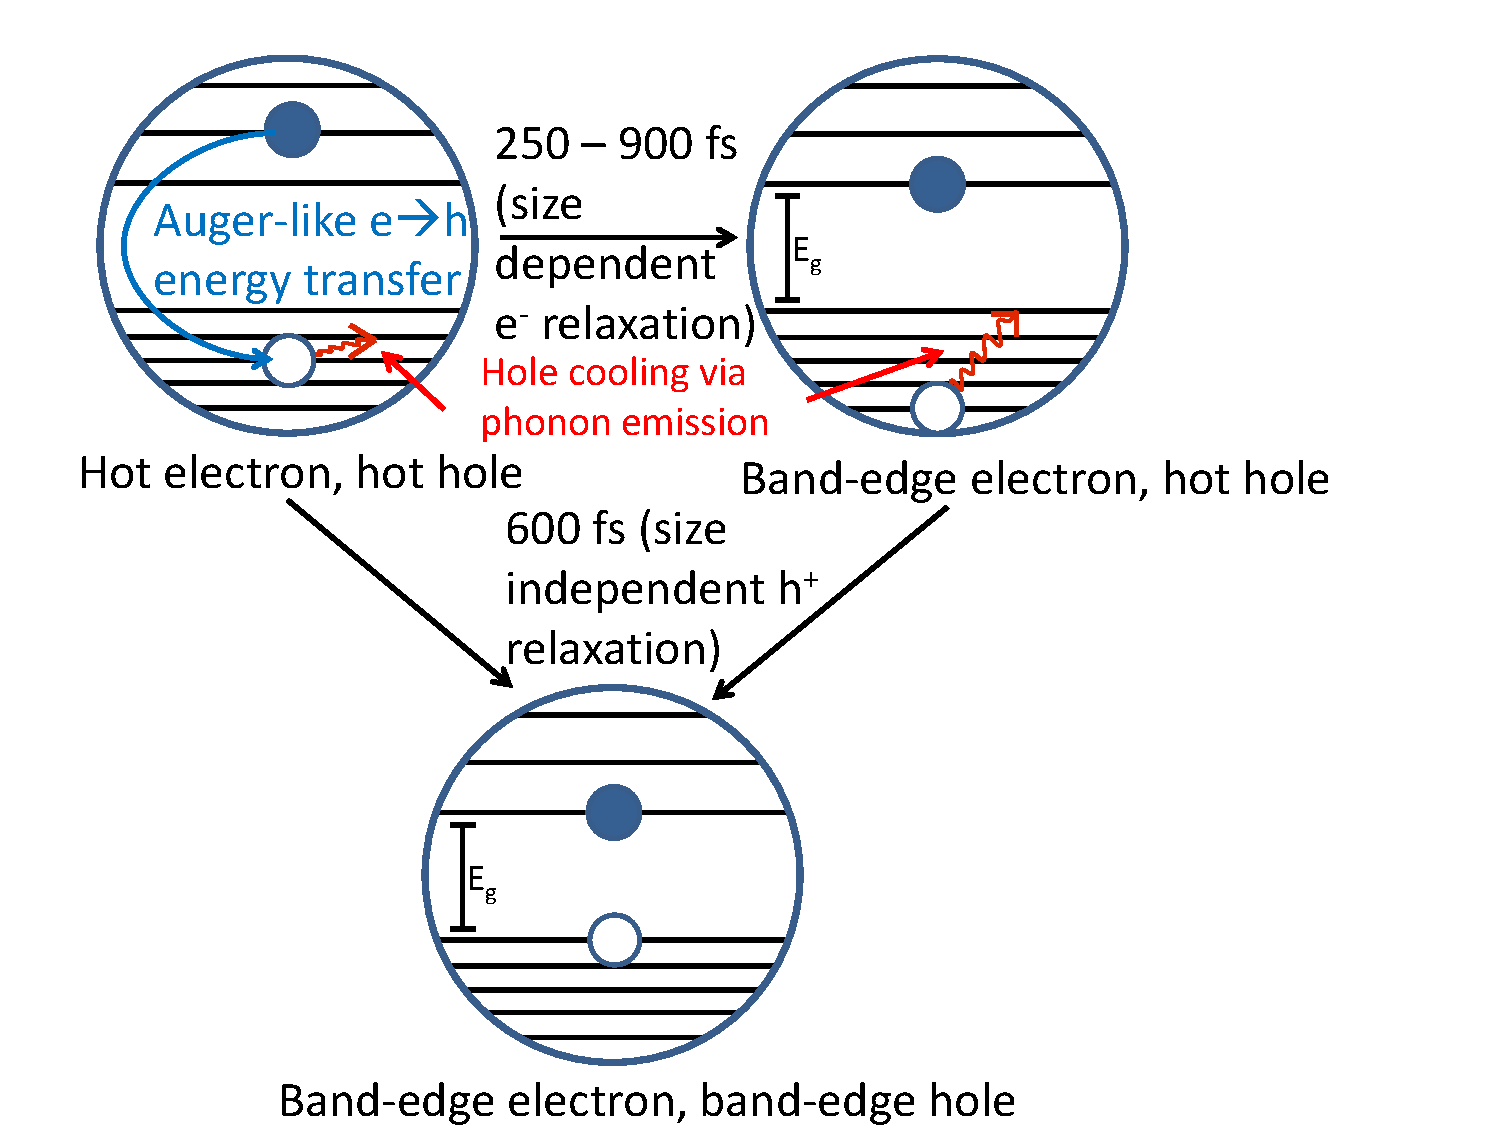
\includegraphics[width=\textwidth]{./Chapter2/fsrs4.pdf}
\caption[Schematic depiction of carrier thermalization in CdSe NCs.]{Following photoexcitation, Auger energy transfer provides the primary relaxation pathway for the electron. Auger energy transfer rates are dependent on NC size. Conversely, hole cooling is primarily facilitated by LO phonon generation, a process with little or no dependence on NC size for CdSe.}
\label{f:fsrs4}
\end{center}
\end{figure}

\section{Electron-Phonon Thermalization in Metallic Nanostructures}
\subsection{Introduction}
While the majority of this thesis is focused on semiconductor systems, we have also explored analogous thermalization processes in small ($\sim$4 nm diameter) gold nanoparticles (Au NPs).  Specifically, we have utilized \emph{ab-initio} atomistic modeling to study the impact of surface chemistry on electron-phonon thermalization in these systems. Overall, we find that electron-phonon thermalization lifetimes (hereafter referred to as $\tau_{ep}$) vary by $\sim$20\% as a function of surface chemistry for otherwise identical systems. Our electronic structure calculations permit us to attribute this variance to an increased electronic heat capacity owing to modification of the DOS near the Fermi level of gold ($E_F$).  

\subsection{Background and Experimental Results}
Numerous existing works suggest a possible impact of chemical passivation on the lifetime of hot electrons in Au NPs \cite{westcott2001adsorbate,hu2002heat,huang2007effect,link2002hot,shin2003comparative}, but the specific mechanism by which the surrounding environment influences the thermalization of hot electrons remains unclear. \par

As a representative example, Figure \ref{f:gold1} shows the transient absorption spectra of 0.7 $\mu$M solutions of aminated and thiolated Au NP samples in toluene at a series of time delays following photoexcitation. These spectra were acquired under pump fluences adjusted to fix the average number of absorbed photons per particle, $\left\langle N\right\rangle$, after accounting for differences in the extinction coefficient between the two samples. Experimental work in this section was carried out by Kenneth Aruda and Christina Sweeney (Department of Chemistry, Northwestern University), and further experimental details may be found in the work by Aruda \emph{et al} \cite{aruda2013identification}. \par

\begin{figure}
\begin{center}
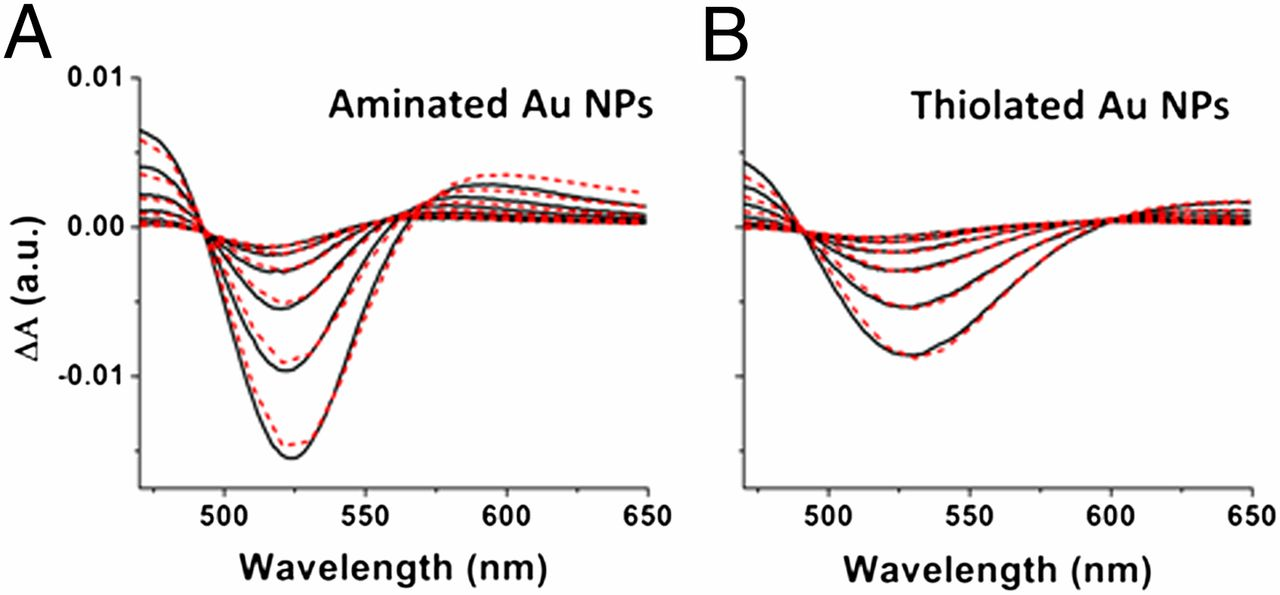
\includegraphics[width=\textwidth]{./Chapter2/gold1.jpg}
\caption[Representative transient absorption spectra of aminated and thiolated Au NP samples.]{Representative transient absorption spectra of aminated (A) and thiolated (B) Au NP samples ($\left\langle N\right\rangle = 2$ photons per particle) at a series of time delays after photoexcitation: 1.5 - 4.5 ps, with 0.6 ps intervals. The dashed red lines are the best fits to each differential spectrum with temperature dependent Mie theory using fixed and floating parameters, as described in the work by Aruda \emph{et al.} \cite{aruda2013identification} From each fit the electronic temeperature of the system may be extracted for the corresponding time delay. Transient absorption data courtesy of Ken Aruda, Weiss lab, Department of Chemistry, Northwestern University.}
\label{f:gold1}
\end{center}
\end{figure}

The time dependence of the TA spectrum can be converted to a time-dependent electronic temperature via fitting of the spectra to temperature-dependent Mie theory \cite{scaffardi2006size,rosei1973d,inouye1998ultrafast}. While the details of the fitting procedure are reported in the literature \cite{aruda2013identification}, the results are summarized in Figure \ref{f:gold2}. Figure \ref{f:gold2} displays the time-dependent electronic temperature following photoexcitation for aminated and thiolated Au NPs. Previous work on electronic cooling in gold has determined that the dynamics on the 300 fs timescale correspond to electron-electron thermalization, while dynamics on the 1-5 ps timescale correspond to thermalization between electronic and vibrational degrees of freedom in the system. Longer decays reflect the dissipation of heat into the solvent bath \cite{link2002hot}. \par

\begin{figure}
\begin{center}
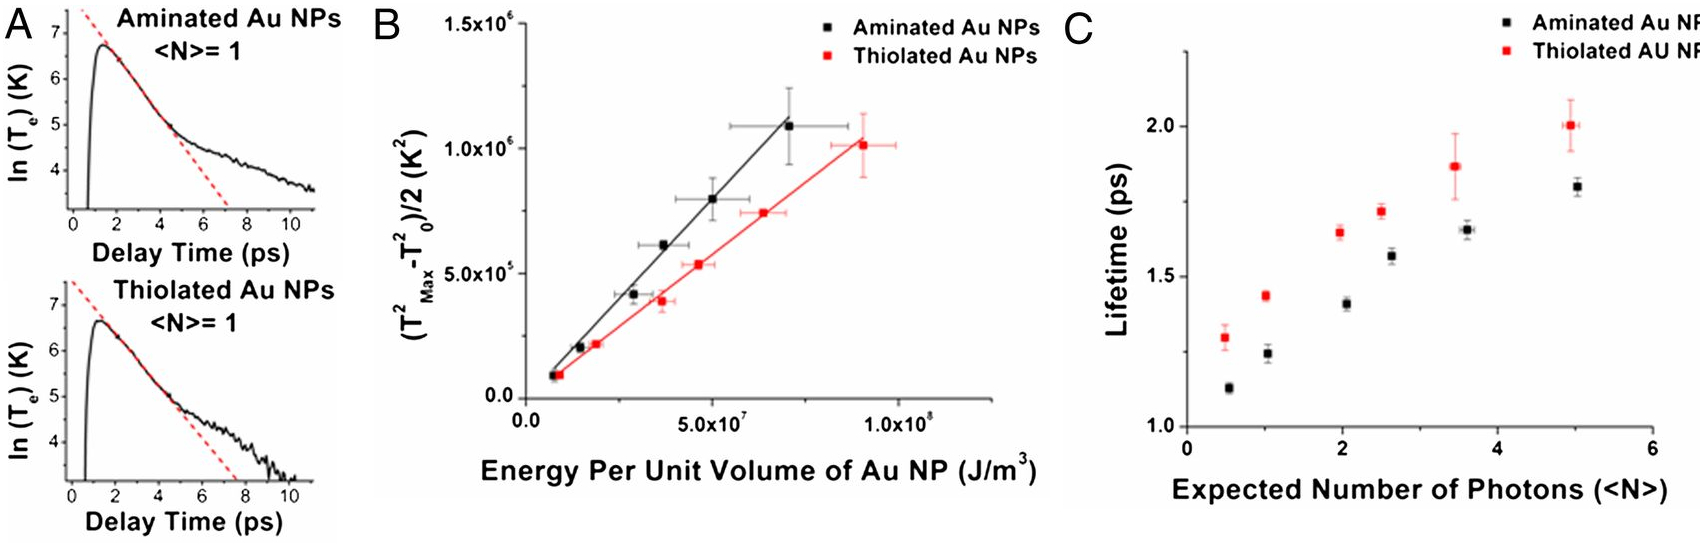
\includegraphics[width=\textwidth]{./Chapter2/gold2.jpg}
\caption[Measurements of hot electron cooling parameters for thiolated and aminated gold nanoparticles.]{(A) The electronic temperature of the thiolated (top) and aminated (bottom) Au NP-ligand systems, determined by fitting the TA spectra as a function of time (\ref{f:gold1}). The kinetic traces show an initial thermalization period caused by electron-electron scattering ($t < 300$ fs) followed by a period in which the hot electron gas equilibrates with vibrational degrees of freedom in the system ($t = 1-5$ ps), and a final period in which the vibrational modes associated with the Au NP dissipate energy into the solvent. The red lines display linear fits to the electron-phonon thermalization regime assuming a first-order decay of the electronic temperature. (B) The square of the initial electronic temperature of the system (following electron-electron scattering) minus the square of the electronic temperature prior to photoexcitation, plotted against the energy of laser normalized by Au NP volume. The slope of this line is inversely proportional to the electronic heat capacity constant for the Au NPs (see Equation \ref{eq:goldeq1}). (C) The observed electron-phonon thermalization lifetime ($\tau_{ep}$) as a function of $\left\langle N\right\rangle$. Expectation values were calculated assuming extinction coefficients of 4.71 $\times$ $10^6$ M$^{-1}$cm$^{-1}$ for the aminated NPs and 3.07 $\times$ $10^6$ M$^{-1}$cm$^{-1}$ for the thiolated NPs at 520 nm. Transient absorption data courtesy of Ken Aruda, Weiss lab, Department of Chemistry, Northwestern University.}
\label{f:gold2}
\end{center}
\end{figure}

The dynamics in Figure \ref{f:gold2}(a) allow us to extract the electronic heat capacity of the system, $\gamma T_e$, where $\gamma$ is the electronic heat capacity coefficient and $T_e$ is the electronic temperature. Experimentally, the electronic heat capacity is related to the energy absorbed by the laser pulse, $U$, \emph{via} $T_e^{max}$, which is the temperature of the electronic system immediately following electron-electron thermalization: \par
\begin{equation}\label{eq:goldeq1}
U = \int_{T_0}^{T_e^{max}}\gamma T_e \mathrm{d}T_e = \frac{1}{2}\gamma(T_e^{max^2} - T_0^2)
\end{equation}
In Eq. \ref{eq:goldeq1}, $T_0$ = 298 K, the initial temperature of the system. Figure \ref{f:gold2}(b) displays the maximum increase in electronic temperature for given values of $U$ for aminated and thiolated Au NPs. These results reveal an elevated $T_e^{max}$ for aminated particles. Given that $T_e^{max}$ is inversely proportional to $\gamma$ (see Eq. \ref{eq:goldeq1}), these results suggest an elevated heat capacity for thiolated particles. \par

Fitting the dynamics in Fig. \ref{f:gold2}(a) to a first-order exponential decay, we may extract the electron-phonon thermalization time constant, $\tau_{ep}$. These extracted lifetimes are displayed as a function of $\left\langle N\right\rangle$ in Fig. \ref{f:gold2}(c). Electron-phonon thermalization times are systematically elevated by $\sim$20\% for thiolated particles relative to aminated particles.

\subsection{Computational Modeling}
In an effort to understand the physical mechanism underlying surface-based modification of the electronic heat capacity, we performed DFT calculations on thiolated and aminated Au slabs.  To prepare initial geometries for DFT calculations, a 5-layer slab of fcc gold having an exposed (111) surface was passivated in four sites on the surface with either methylamine or ethylthiolate. In the methylamine case, the binding geometry found by Trout \emph{et al.} for a gold surface was used as a starting point for the geometry relaxation \cite{pong2005first}. In the case of ethylthiolate, ligands were bound to the (111) surface through a gold ad-atom in a "staple" motif, known to be an extremely stable binding arrangement for both Au (111) surfaces and Au NPs \cite{voznyy2009c,pensa2012chemistry}. Carbon and hydrogen atom positions were initially relaxed using molecular mechanics with the universal force field, as implemented in the Avogadro 1.1.0 software \cite{hanwell2012avogadro}. Following relaxation of the C and H positions, the surfaces of the gold slab with ligands were relaxed within the DFT framework as implemented in the Amsterdam Density Functional (ADF) 2010.01 program. Specifically, atomic positions were relaxed until the force on each atom was less than 0.02 eV/\r{A}, with gold atoms beneath the first two surface layers having fixed positions. All electronic structure calculations utilized the BP86-D GGA exchange correlation functional with a triple-zeta potential basis set having a single polarization function.  To describe core electrons in gold atoms, a 4f frozen core approximation was applied and scalar relativistic effects were incorporated using the zeroth-order regular approximation. In all density of states (DOS) plots, the Fermi level of gold has been set as the zero of energy.  Electronic structure calculations yield a "stick" spectrum of discrete eigenvalues, which are broadened using a Gaussian broadening function with a width of 0.02 eV to yield the DOS spectra reported here. \par

\begin{figure}
\begin{center}
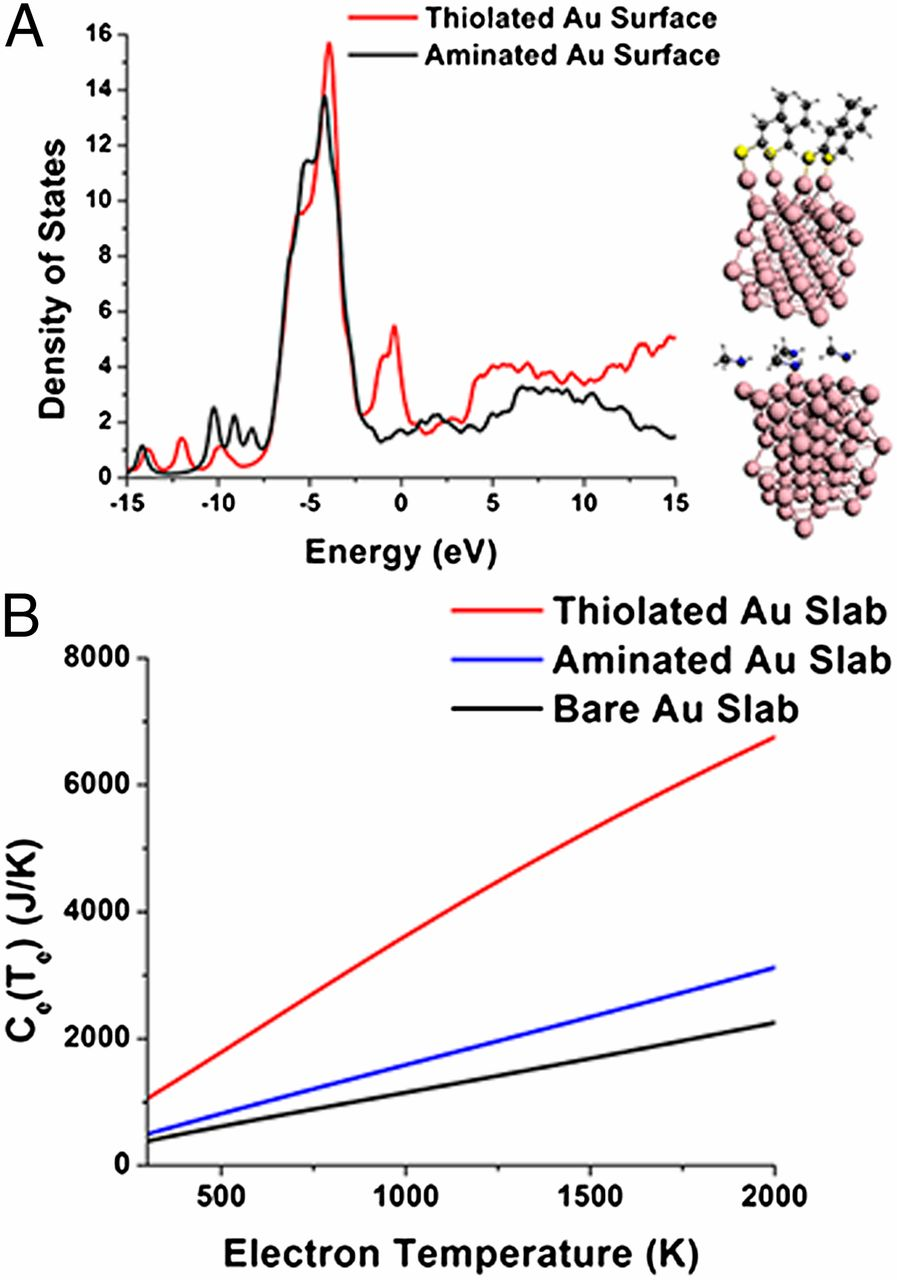
\includegraphics[width=0.5\textwidth]{./Chapter2/gold3.jpg}
\caption[Electronic structure calculations on Au-ligand model systems.]{(A) Density of electronic states as a function of energy for the Au slabs passivated with amines and thiolates (Right). Note that the aminated and thiolated clusters have different state density at the Fermi level (0 eV). Each surface atom on the Au slab is bound to a ligand, such that each cluster in the simulation has the same number of ligands. (B) Calculated electronic heat capacities for the ligated Au slabs in A reproduce the linear dependence of heat capacity on temperature predicted by Eq. \ref{eq:goldeq2}, as well as a dependence of the electronic heat capacity on the electronic DOS at the Fermi level of the Au NP-ligand system.}
\label{f:gold3}
\end{center}
\end{figure}

Figure \ref{f:gold3}(a) shows the electronic DOS of Au slabs functionalized with thiols and amines calculated with DFT. Figure \ref{f:gold3}(b) shows a calculation of the electronic heat capacity, $C_e(T_e)$ for amine- and thiolate-passivated Au slabs using the DFT-derived electronic DOS along with a semiclassical expression for electronic heat capacity as follows \cite{lin2008electron}:
\begin{equation}\label{eq:goldeq2}
C_e(T_e) = \int_{-\infty}^{\infty}\frac{\mathrm{d}f(\varepsilon,\mu,T_e)}{\mathrm{d}T_e}DOS(\varepsilon)\varepsilon\mathrm{d}\varepsilon
\end{equation}
In Eq. \ref{eq:goldeq2}, the function $f(\varepsilon, \mu, T_e)$ is the Fermi-Dirac distribution as a function of energy ($\varepsilon$), chemical potential ($\mu$), and electronic temperature ($T_e$). The results in Fig. \ref{f:gold3}(b) show that the heat capacity for thiolated Au NPs is roughly twice that displayed by the aminated Au NPs, as expected from the increased DOS in the vicinity of the Fermi level (Fig. \ref{f:gold3}(a)) and in general agreement with the results presented in Fig. \ref{f:gold2}. However, quantitative comparisons with experiment are complicated by the elevated ligand-to-gold ratio in the thin slab model used here relative to the Au NPs studied experimentally. The more modest increase in electronic heat capacity observed experimentally may also be understood by considering the effect of electronic structure modifications on electron-phonon coupling. \par

From these electronic structure calculations, we are also able to explore the impact of electronic DOS on the temperature-dependent electron-phonon coupling, $G(T_e)$, as expressed in Equation \ref{eq:goldeq3}:
\begin{equation}\label{eq:goldeq3}
G(T_e) = \frac{\pi\hbar k_B\lambda\left\langle\omega^2\right\rangle}{DOS(E_F)}\int_{-\infty}^{\infty}\frac{\mathrm{d}f(\varepsilon,\mu,T_e)}{\mathrm{d}\varepsilon}DOS^2(\varepsilon)\mathrm{d}\varepsilon
\end{equation}
In Eq. \ref{eq:goldeq3}, $\left\langle\omega^2\right\rangle$ is the second moment of the phonon spectrum and $\lambda$ is the electron-phonon mass enhancement parameter; both parameters are material dependent and assumed here to be bulk Au values. Figure \ref{f:gold4} shows the calculated electron-phonon coupling constants for bare, aminated, and thiolated Au slabs. The thiolated gold slabs, possessing an elevated DOS near $E_F$, exhibit a larger coupling constant than either bare or aminated surfaces. Intuitively, one expects that elevated electron-phonon coupling should facilitate more rapid electron-phonon thermalization, partially offsetting the effects of elevated electronic heat capacity described above.

\begin{figure}
\begin{center}
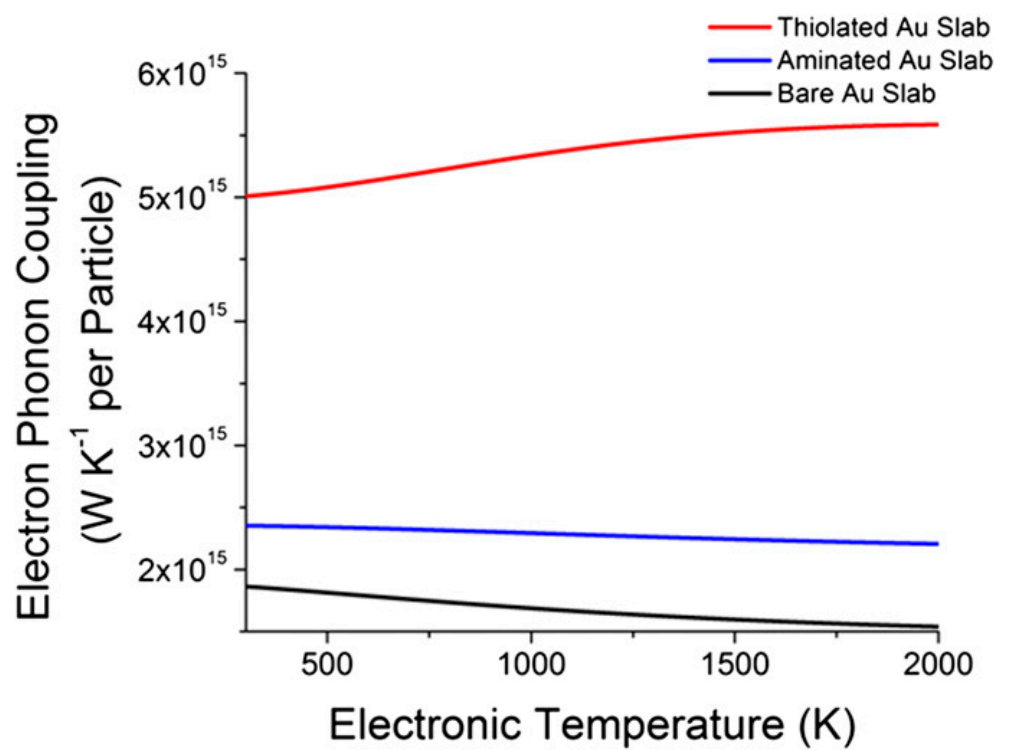
\includegraphics[width=0.75\textwidth]{./Chapter2/gold4.png}
\caption[Simulated electron-phonon coupling constants for thiolated and aminated Au slabs as a function of temperature.]{Simulations of the electron-phonon coupling constant calculated with the electronic density of states determined by DFT of gold slabs. The thiolated
Au slabs with higher DOS at the Fermi level show a larger electron-phonon coupling than both the aminated and bare Au slabs.}
\label{f:gold4}
\end{center}
\end{figure}

\subsection{Conclusions}
Electronic structure calculations were used to explore the impact of surface chemistry on electronic heat capacity and electron-phonon coupling in nanoscale gold structures, which exhibit a dependence (previously) poorly understood dependence on the identity of the passivating chemical species. Motivated by transient absorption measurements demonstrating elevated electron-phonon thermalization times for thiol-passivated Au NPs as compared to aminated Au NPs, we carried out DFT calculations on model Au systems passivated by both types of ligands. These results permit an \emph{ab-initio} calculation of the electronic heat capacity and electron-phonon coupling constant. Thiolated Au slabs were found to exhibit a much larger density of states in the vicinity of the Fermi level, resulting in an elevated electronic heat capacity and electron-phonon coupling constant (see Eqs. \ref{eq:goldeq2} and \ref{eq:goldeq3}).

The larger electronic heat capacity of thiolated Au NPs translates into a smaller driving force for energy exchange between electron and vibrational populations for a given initial electron temperature, and therefore a slower electron cooling process, for thiolated NPs than for aminated NPs. This effect is counteracted by the larger electron-phonon coupling for thiolated NPs than aminated NPs, because electron-phonon coupling increases the rate of energy transfer from electronic states to vibrational states. The increase in both $g$ and $\gamma$ upon exchanging amines for thiolates is not coincidental; both quantities are positively correlated with the electronic DOS near the Fermi level of the NP-ligand system. Overall, our calculations provide microscopic insight into the physical mechansims underlying the observed $\sim$20\% increase in electron-phonon thermalization times in thiol-covered Au NPs.

\chapter{Characterization of Heat Transport in Nanometer Scale Systems}

Work presented in this chapter is adapted from the following papers:

\begin{itemize}
\item Hannah, D. C.; Dunn, N. J.; Ithurria, S.; Talapin, D. V.; Chen, L. X.; Pelton, M.; Schatz, G. C.; Schaller, R. D. \emph{Phys. Rev. Lett.} \textbf{2011}, 107, 177403

\item Hannah, D.C.; Gezelter, J.D.; Schaller, R.D.; Schatz, G.C. \emph{ACS Nano} \textbf{2015}, 9, 6278
\end{itemize}
\section{Introduction}

Colloidal semiconductor nanocrystal (NC) quantum dots offer size-tunable band gaps, solution processing, and controllable surface functionality that can impact technologies ranging from lighting \cite{doi:10.1021/nl9002969} and biolabels \cite{doi:10.1146/annurev.bioeng.7.060804.100432} to photovoltaics \cite{Huynh29032002} and thermoelectrics \cite{Hsu06022004, Talapin07102005}.  While much of the materials community focuses on new compositions as well as determination of NC optical properties and incorporation into devices, thermal management, which is crucial to each of the highlighted technologies, will become an increasingly important factor for the use of these thermodynamically compromised materials. Measurement and manipulation of thermal outflow rates in nanoscale semiconductors at present, however, represents a challenge. Comprehensive understanding of the electron-hole pair (“exciton”) dynamics, electronic structure, and thermal properties of such designer materials in aggregate is vital to their successful application.  In this Chapter, we detail an optical signature of phonon outflow from matrix-embedded semiconductor nanocrystals via observation of transient phonon-assisted radiative recombination from the lowest-energy exciton fine structure state (the "dark" exciton state), for which transitions are ordinarily dipole-forbidden. We also utilize a recently-developed MD method to simulate thermal transport at a realistic, chemically passsivated semiconductor/ligand/solvent interface and determine the role played by the ligand layer as well as the crystal structure of the underlying semiconductor in mediating thermal transport rates at this interface.

\subsection{Experimental Challenges}

From a fundamental point of view, the small size of NCs challenges predictions and measurements of thermal transport. While NC radii generally range in size from 1 to 40 nm, phonon mean free paths are typically hundreds of nanometers. Such discrepancy in sizes yields highly diffusive scattering, wherein phonons scatter in all directions upon interaction with a NC interface \cite{chen2000particularities}. Small NC sizes also present experimental challenges.  Technique-specific sample length and size requirements that greatly exceed NC diameters rule out contact-based measurements including hot-wire probes and the $3\omega$ method \cite{chen2000particularities, PhysRevLett.95.065502}. Noncontact probes such as transient absorption permit studies of phonon outflow from metallic nanoparticles via the thermal-broadening of plasmon resonances, but such measurements are not applicable to semiconductor NCs \cite{pelton2009damping,doi:10.1021/jp020581+,pelton2009damping}. Transient thermoreflectance (TTR) uses an optical pump to heat a reflective surface and a time-delayed probe to track temperature induced changes to the reflectivity of the surface \cite{paddock1986transient}. Along with fits to an appropriate thermal transport model, this method is capable of optically measuring thermal conductivity as well as interfacial thermal conductance, and has been successfully applied to densely packed NC films \cite{ong2013surface}. However, such measurements probe surface areas containing tens of thousands of NCs and inherently relay only averaged information about thermal transport. \par

Isolated particles (either suspended as a colloid or in a matrix) can provide information about particle-level thermal transport but do not provide a reflective surface for TTR to be carried out. Colloidal semiconductor materials that present a continuous density of states (DOS), such as one-dimensional quantum confined rods, permit the measurement of thermally populated electronic states \cite{achermann2006effect}; however zero-dimensional NCs exhibit a discrete DOS that prevents utilization of this approach. Examinations of intraband electronic relaxation \cite{PhysRevB.60.R2181,PhysRevLett.80.4028} and coherent phonons \cite{1464-4258-10-6-064004,PhysRevLett.79.5102,PhysRevB.77.235321} in semiconductor NCs suggest that excess carrier energy produces phonons on an ultrafast time scale, but the fate of these phonons remains elusive. Even in cases where coherent phonons are observed, the damping of coherent oscillations likely reflects dephasing in the NC ensemble owing to size polydispersity (each nanocrystal has a slightly different vibrational frequency) rather than actual changes in phonon population.

\subsection{Theoretical Challenges}

Chen and co-workers, among others, note fundamental difficulties associated with applying current heat conduction theories to structures in this size regime \cite{chen2000particularities}. As described in the introduction to this thesis, the extent to which approximations for the phonon distribution function and transmission coefficients apply to the case of chemically passivated interfaces is unclear. While simple, the acoustic mismatch model (AMM) assumes specular reflection/transmission of interfacial phonons - likely a poor assumption for rough interfaces \cite{chen2000particularities} - and at any rate, the acoustic properties of the passivating monolayer are not well characterized or understood for most common materials. The diffuse mismatch model (DMM) is perhaps somewhat more intuitively appealing for an interface displaying at least one highly disordered component. However, it assumes phonon scattering is completely diffuse, i.e. that phonons lose all "memory" of their trajectory upon scattering. This results in transmission probability lacking any dependence on phonon wavevector, which may be a poor approximation for the crystalline side of the interface. Indeed, DMM-based predictions of interfacial thermal conductance often significantly over- or underestimate interfacial thermal conductance at non-cryogenic temperatures \cite{yang2015thermal, duda2009extension}, depending on the materials present. \par

While extensions of the DMM to account for higher temperatures \cite{duda2009extension}, interfacial disorder \cite{beechem2007role}, and inelastic scattering \cite{hopkins2007effects} have improved the accuracy of the model, problems persist related to the assumption of completely diffusive scattering. Furthermore, these developments have focused on interfaces which are roughly planar, and they may not be extensible to a nanoparticle. Instead, we model thermal transport in the systems of interest here using classical MD simulations, which avoid problematic assumptions about the nature of phonon-phonon scattering and are fully atomistic, allowing us to account for specific chemical details. Additionally, MD simulations are computationally inexpensive and generally highly parallelizable, allowing for the treatment of experimentally-sized systems. Because of these factors, MD simulations have become the standard method of theoretically evaluating interfacial thermal conductance \cite{cahill2003nanoscale, yang2015thermal, cahill2014nanoscale}. Classical MD simulations do exhibit the significant of limitation of equipartitioning - that is, each vibrational mode in the system is equally excited. This equipartitioning requirement arises from thermostats which enforce statistical sampling from a specific ensemble (i.e. NVT - constant number of particles (N), volume (V), and temperature (T) or NPT - constant N, pressure (P) and T) and calculate the kinetic energy of the system according to the equipartition theorem. While semiclassical methods accounting for quantum effects in molecular vibrations are an active area of research \cite{PhysRevB.79.224305, PhysRevB.86.064305}, in principle they are not necessary here because we are simulating temperatures above the Debye temperature of CdSe. Thus, all of the vibrations involved in interfacial thermal conductance are expected to be thermally populated in the physical system and should be well approximated by a MD simulation with equipartitioning. We present specific details of MD-based treatements of interfacial thermal conductance later in this chapter. 

\section{Streak Camera Measurements}

Many of the experimental results presented in Chapters 3-5 hinge on the unique detection capabilities afforded by a streak camera. Single-photon sensitive streak cameras yield simultaneous spectral and temporal resolution on up-to single picosecond timescales (as is the case with our experimental setup). An example of streak camera operation is shown in Figure \ref{f:streakcam}. \par

\begin{figure}
\begin{center}
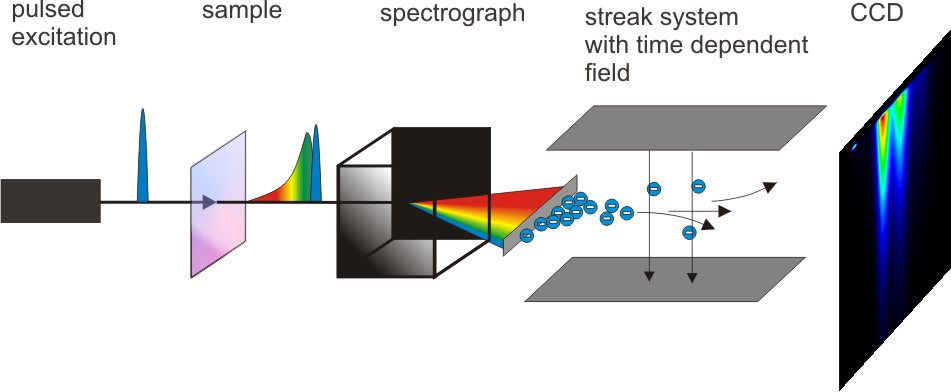
\includegraphics[width=0.75\textwidth]{./Chapter4/streakcam.jpeg}
\caption[Diagram of streak camera detection scheme.]{Following pulsed excitation of an emissive sample, PL photons are dispersed using a spectrograph and "streaked" across a CCD using a time dependent applied voltage sweep.}
\label{f:streakcam}
\end{center}
\end{figure}

Streak camera measurements are carried out utilizing a pulsed excitation source. First, a laser pulse excites a luminescent sample. Subsequent to photoexcitation, emitted PL photons are collected and spectrally resolved by a spectrograph. These photons are then directed through a streaking cathode onto a phosphor screen, producing flashes detected by a CCD. The streaking cathode utilizes a time-dependent voltage sweep synchronized with the laser excitation. As a result, electrons strike the target phosphor at a distinct and precise height which depends on the time after photoexcitation that they entered the streak cathode. The net result is a temporally and spectrally resolved image which may be binned vertically and horizontally to yield PL decay dynamics or time-resolved emission spectra, respectively.


\section{Observation of Acoustic Phonon Transport Using Ultrafast Photoluminescence Spectroscopy}

Significant information exists for CdSe NCs regarding carrier dynamics and electronic structure, the relevant findings of which we summarize here. Following photoexcitation, excitonic intraband relaxation down to the “band-edge” states takes place on subpicosecond to single-picosecond time scales \cite{PhysRevLett.80.4028, PhysRevB.60.R2181, PhysRevLett.96.057408}.  Radiative recombination, on the other hand, requires tens to hundreds of nanoseconds and exhibits strong temperature dependence owing to both details of the size- and shape-specific exciton fine structure as well as exciton-phonon interactions \cite{:/content/aip/journal/jcp/96/2/10.1063/1.462114, PhysRevLett.75.3728, PhysRevB.54.4843, PhysRevB.60.1819, :/content/aip/journal/apl/82/17/10.1063/1.1570923, doi:10.1021/jp051738b, PhysRevB.74.085320,PhysRevLett.102.177402}.  Crystal field effects, spin-orbit coupling, and the electron-hole exchange interaction \cite{PhysRevB.54.4843, PhysRevB.60.1819} give rise to the energetic ordering and size-dependent energy spacings of the band-edge exciton states. A dipole forbidden (optically passive or “dark”) lowest-energy exciton, with spin projection $J = \pm 2$ along the wurtzite c axis, resides below an optically allowed (bright, $J = \pm 1$) exciton state by 2 - 17 meV, with larger dark-bright splittings ($\Delta_{db}$) for smaller NC sizes \cite{PhysRevLett.75.3728}.  At cryogenic temperatures, insufficient thermal energy exists to populate the lowest-energy bright exciton state, and microsecond lifetimes result due to the weakly emissive character of the dark exciton. By contrast, at higher temperatures, a thermal (Boltzmann) population of bright excitons radiates with an established lifetime of $\sim 20$ ns \cite{:/content/aip/journal/apl/82/17/10.1063/1.1570923}.  Nirmal \emph{et al.} established values of $\Delta_{db}$ from the energy difference between a spectrally narrow excitation laser and the proximal, zero-phonon PL (PL) peak position owing to spin-forbidden recombination from dark excitons \cite{PhysRevLett.75.3728}.  The same study found LO-phonon-assisted emission bands at lower energy wherein emission of a photon and generation of an LO phonon yields momentum-conserving transitions from the dark state. Magnetic fields were found to quantum mechanically mix proximal bright and dark states, which increases the zero-phonon amplitude relative to the LO-phonon-assisted feature and yields a notable increase in the radiative recombination rate \cite{PhysRevLett.75.3728}.  Also, cryogenic four-wave mixing measurements suggest that optically bright photoexcited excitons decay into lowest-energy dark exciton states roughly in the same time as intraband relaxation \cite{PhysRevB.73.125322}.  \par

In this section, we examine a long-standing, poorly understood feature in CdSe NC dynamics and attribute it to thermal dissipation. Specifically, in addition to the more fully characterized dark and bright radiative lifetimes, Crooker showed that low-temperature time-resolved PL (trPL) measurements exhibit an unusual, rapid initial decay for sample temperatures below $\sim 20$ K, signatures of which appear in numerous reports \cite{:/content/aip/journal/jcp/96/2/10.1063/1.462114, :/content/aip/journal/apl/82/17/10.1063/1.1570923, doi:10.1021/jp051738b, PhysRevB.74.085320, PhysRevLett.102.177402}.  To date, this fast burst of PL has remained uncharacterized due to an instrumental lack of sufficient temporal resolution. We temporally and spectrally resolve this feature, revealing clear size-dependent dynamics as well as distinct spectral characteristics that, taken together in the context of literature from metals and semiconductors, permit us to assign the feature to size-dependent thermal outflow. While low temperatures are required in order to observe this outflow, the thermal transport constants may be scaled to temperatures of relevance to device applications.  \par

We examine several sizes of CdSe NCs capped with octadecylamine, which exhibit PL quantum yields in excess of 20\% at room temperature. Small discrepancies exist regarding available CdSe sizing curves (used to convert absorption maximum to NC radius), but these did not qualitatively impact presented results. NCs were dispersed in a 1:1 octadecane:eicosane solvent and dripped onto a sapphire substrate. The samples were loaded into a closed-cycle helium cryostat and photoexcited with 35 fs pulses from a 2 kHz amplified Ti-sapphire laser at 3 eV. The excitation fluence utilized corresponds to the production of less than 0.05 electron-hole pairs per NC per pulse, and results were unchanged for 3$\times$ higher or lower excitation intensities. PL photons were directed to a 150 mm spectrograph and streak camera. Detector regions were binned vertically or horizontally to produce time-resolved spectra or spectrally resolved dynamics, respectively. \par

A streak camera image recorded at 2.6 K [Fig. \ref{f:trpl1}(a)]  for the first few hundred picoseconds following photoexcitation of a 1.6-nm-radius NC sample (556 nm 1S absorbance maximum) shows a fast initial burst of emission that is not distinct at 80 K [Fig. \ref{f:trpl1}(b)], in qualitative agreement with previous reports that did not spectrally or temporally resolve this feature \cite{:/content/aip/journal/apl/82/17/10.1063/1.1570923, doi:10.1021/jp051738b, PhysRevB.74.085320, PhysRevLett.102.177402}.  At 2.6 K, time-resolved spectra [Fig. \ref{f:trpl1}(c)] exhibit shorter wavelength PL during the first $\sim$ 80 ps following excitation which redshifts to a constant value for longer times, whereas the 80 K sample temperature lacks any pronounced spectral shift over the same time range. Dynamics in Figs. \ref{f:trpl1}(e) and \ref{f:trpl1}(f) display a fast relaxation feature at 2.6 K for bluer wavelengths that is largely absent from the redder PL at 2.6 K and is absent for all wavelengths in the 80 K data. \par

\begin{figure}
\begin{center}
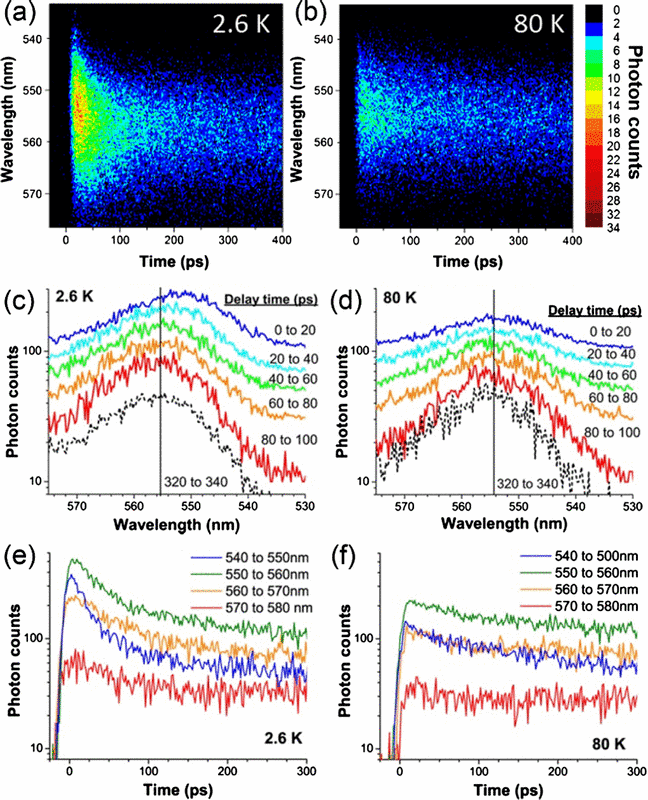
\includegraphics[width=0.75\textwidth]{./Chapter4/trpl1.png}
\caption[Spectra and dynamics of PL at 3K and 80K from an ensemble of CdSe NCs.]{(a) Temporally and spectrally resolved single exciton PL from a 1.6-nm-radius CdSe NC ensemble at 2.6 K and (b) at 80 K. Here, lower sample temperature results in a faster emission feature as well as a spectral shift to lower energy with time. (c),(d) Time-resolved spectra collected at the indicated temperatures and binned over the indicated time delays reveal a redshift with increasing time at 2.6 K that is not observed at 80 K. Spectra are linearly offset for clarity. The black vertical lines indicate the peak emission amplitude of the 320-340 ps time-binned spectrum. (e),(f) Spectrally resolved PL dynamics become biexponential for shorter PL wavelengths in the case of the lower sample temperature.}
\label{f:trpl1}
\end{center}
\end{figure}

Single Gaussian fits of the ensemble-broadened spectra shown in Fig. \ref{f:trpl1}(c) yield similar full width at half maximum linewidths (16.2 nm for $t = 0 - 20$ ps and 17.3 for $t = 320 - 340$ p), which suggests that a single population evolves to emit with reduced energy over time. For the dynamics collected at 2.6 K in Fig. \ref{f:trpl1}(e), we find that the decay on the blue side of the PL is well-described by a biexponential decay, while the redder PL dynamics at low temperature and all of the dynamics recorded at 80 K appear single exponential in the time window examined. The biexponential fit time constants differ by more than 1 order of magnitude, which allows for highly independent fits. While the spectrally resolved dynamics in Fig. \ref{f:trpl1}(e) each exhibit fast decay constants that differ by $\sim$25\% for proximal spectral slices (slower for lower-energy PL), most of the fast-component amplitude is present in a narrow spectral region. To systematically compare data for different samples, we hereafter bin all trPL to the blue of the time-integrated PL spectral maximum so as to yield characteristic (“blue-side”) dynamics of the higher energy, prompt emission. \par

In Fig. \ref{f:trpl2}, we display temporally resolved blue-side decay dynamics, normalized at late times, for multiple NC sizes at both 2.6 and 80 K. For each sample, the low-temperature dynamics become faster and biexponential in comparison to the slower single exponential decays recorded at high temperature. We summarize two general trends in \ref{f:trpl3}: The blue side becomes progressively longer-lived as the NC radius increases, and the spectral shift associated with the fast decay feature yields a roughly constant value of $\sim$25 meV irrespective of NC size (inset).  The fast decay lifetime plotted vs NC radius squared exhibits a linear relationship. While such a trend has not been reported previously for a semiconductor NC composition, a comparable relation has been found in metal nanoparticles \cite{doi:10.1021/jp020581+, PhysRevB.66.224301} and is attributed to particle thermalization rates as dictated by interfacial and thermal diffusion \cite{doi:10.1021/jp020581+, PhysRevB.66.224301,doi:10.1021/jp048375k}. \par

\begin{figure}
\begin{center}
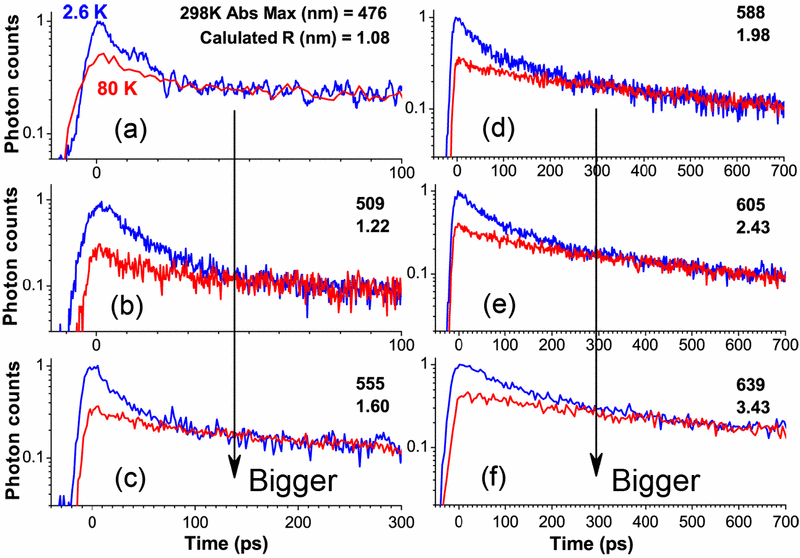
\includegraphics[width=0.75\textwidth]{./Chapter4/trpl2.png}
\caption[High-energy PL decay dynamics for various sizes of CdSe NC at 3K and 80K.]{“Blue-side” radiative recombination dynamics for CdSe samples with indicated radii generated for the higher energy half of the time-integrated PL spectrum at 2.6 (blue lines) and 80 K (red lines). Traces were scaled to overlap at long time. For every sample, the low-temperature trPL data become biexponential. Also, the decay feature appearing at low temperature becomes increasingly faster with reduced NC radius. Note that the tick mark step size is constant (100 ps) for each data panel and that the measured time window is larger for larger NC size.}
\label{f:trpl2}
\end{center}
\end{figure}

\begin{figure}
\begin{center}
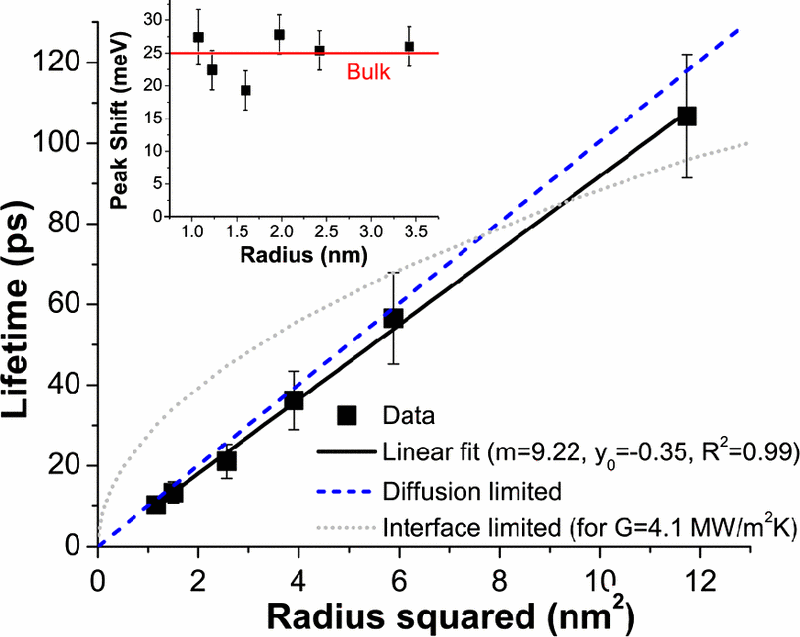
\includegraphics[width=0.75\textwidth]{./Chapter4/trpl3.png}
\caption[Fast pholuminescence feature lifetimes as a function of CdSe nanocrystal radius.]{The faster decay time derived from biexponential fits of the trPL data in Fig. \ref{f:trpl2} (squares) exhibits a linear relationship with the NC radius squared (fitted black solid line). Calculations of diffusion-limited (blue dashed line) and interfacial-conductance-limited (gray dotted line, estimated for an interfacial conductance of 4.1 $MW/m^2K$) dissipation suggest that diffusion controls the measured decay times. The inset displays the energy difference between early recombination and emission subsequent to the fast initial decay. The spectral shifts for multiple NC radii are fairly constant and comparable to the 25-meV LO-phonon energy of bulk CdSe (solid red line). Recombination from higher lying states in the CdSe NC exciton fine structure is not apparent, since such emission would exhibit strong size dependence corresponding to $\Delta_{db}$ values ranging from 2 to 17 meV for the NC size range probed.}
\label{f:trpl3}
\end{center}
\end{figure}

Next, we probe the temperature dependence of the trPL collected for the 1.6-nm-radius sample.  Figure \ref{f:trpl4}(a) shows that the amplitude of the fast decay feature remains unchanged between 2.6 and 10 K but that higher temperatures cause the fast-feature amplitude to decrease. To highlight the evolution of the fast vs slow decay, Fig. \ref{f:trpl4}(b) displays the temperature-dependent ratio of instantaneous PL intensity binned from $t = 0 - 5$ ps divided by that from $t = 200 - 205$ ps for three CdSe NC sizes. Such ratios evolve with temperature similar to Boltzmann thermal partitioning with characteristic energies of 2.2, 1.5, and 1.0 ($\pm$ 0.1) meV for 1.2-, 1.6-, and 2.4-nm radii, respectively, in agreement with calculated lowest-energy acoustic phonon modes in CdSe NCs \cite{PhysRevLett.102.177402, doi:10.1021/nl061414e}. \par

\begin{figure}
\begin{center}
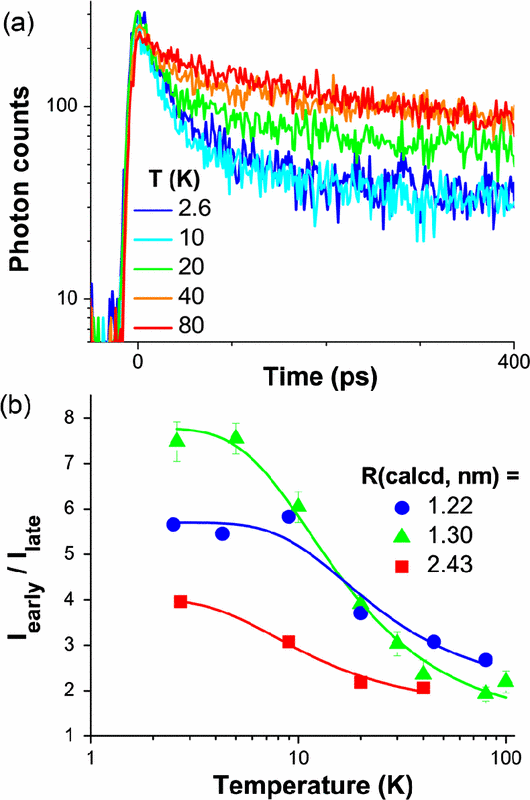
\includegraphics[width=0.65\textwidth]{./Chapter4/trpl4.png}
\caption[Temperature dependent decay of high energy PL from CdSe nanocrystals.]{(a) Increasing sample temperature results in a decrease in amplitude of the fast dynamical component, here for a 1.6-nm-radius CdSe NC sample. (b) The ratio of instantaneous PL intensities integrated from $t = 0 - 5$ ps ($I_{early}$) and from $t = 200 - 205$ ps ($I_{late}$) taken from dynamics such as those shown in (a) for three CdSe NC sizes suggests that Boltzmann populations of low-energy phonons in the NCs eliminates the fast relaxation feature for sufficiently high temperatures. Lines show appropriately scaled thermal partitioning of NCs lacking acoustic phonon excitation, as described in the text. Representative error bars are shown for the 1.30-nm-radius NC sample.}
\label{f:trpl4}
\end{center}
\end{figure}

In the respective contexts of wave packet decoherence and intraband relaxation, Scholes \cite{doi:10.1021/nl061414e, doi:10.1021/nl803275a, :/content/aip/journal/jcp/132/10/10.1063/1.3350871} and Prezhdo and co-workers \cite{doi:10.1021/jp0669052} recently proposed that acoustic phonons transiently mix dark and bright exciton states. In the picture presented by these authors, nonequilibrium acoustic phonons, generated in the current studies as a result of exciton intraband relaxation, mechanically distort the NCs and perturb the fine structure, which increases the oscillator strength of the lowest-energy dark exciton state. At the low temperatures examined in this work, the observed radiative recombination rate diminishes with time as these phonons leave the NCs. By contrast, for higher temperatures, there is a significant equilibrium population of acoustic phonons in the NCs. Furthermore, the increase of the fast-feature amplitude with decreasing temperature, explored in Fig. \ref{f:trpl4} follows the equilibrium thermal partition function describing NCs that lack acoustic phonon population. This relationship suggests that a single, lowest-energy equilibrium acoustic phonon is sufficient to preclude observation of the fast relaxation feature. Subsequent to acoustic phonon dissipation for low temperatures, the radiative rate decreases and LO-phonon-assisted recombination dominates the ensemble PL spectrum, resulting in the size-independent redshift. Acoustic phonon-induced mixing is also consistent with both a notable lack of magnetic circular dichroism at early times following excitation, as reported by Furis et al. \cite{doi:10.1021/jp051738b},  as well as the temperature-dependent radiative recombination rates reported by Oron et al. \cite{PhysRevLett.102.177402} \par

Next we focus on thermal transport estimates, first for a relatively large, 3-nm-radius particle (for which bulk constants may be fairly accurate) and then as a function of NC size. Thermal transport models consider two regimes of heat dissipation: thermal diffusion controlled or interfacial conductivity controlled, each of which can dictate the time scale as well as the functional dependence on NC radius $R$.  We utilize the work of Ge, Cahill, and Braun \cite{PhysRevB.66.224301} to estimate dissipation time scales specific to a CdSe NC suspended in an octadecane matrix initially at 10 K excited with 1 eV of photon energy in excess of the band gap. Modeling the CdSe NC as a Debye solid ($C$ follows $T^3$) reveals that the provided photon excess energy increases the temperature to $\sim$16 K for a 3-nm-radius particle (presented results were insensitive to the initial NC temperature at least within the range of 2.6-10 K).  \par

For large thermal conductivity at the CdSe-alkane interface, thermal diffusion in the medium surrounding the NCs would dictate thermalization time and should follow $\tau_d = \left(C_p\rho_pR\right)^2/9C_m\rho_m\Lambda_m$, where, for the particle ($p$) and matrix ($m$), $C$ is specific heat, $\rho$ is density, and $\Lambda$ is linear thermal conductivity [utilized constants include $C_{p, initial}\left(10 K\right) = 0.012$ J/gK, $C_p\left(16 K\right) = 0.061$ J/gK, $C_m\left(10 K\right) = 0.011$ J/gK, $\rho_p = 5.65$ g/cm$^3$, $rho_m = 0.777$ g/cm$^3$, and $\Lambda_m = 0.0015$ J/cm Ks].  For a 3-nm-radius NC, we estimate a diffusion cooling time under our experimental conditions of 90 ps (close to the interpolated 83 ps).  Figure \ref{f:trpl3} shows close agreement between diffusion-limited cooling times and experiment. \par

In the scenario of rapid diffusion, conductance of heat through the CdSe-alkane interface limits thermalization time, and heat transport would obey $\tau_i = C_p\rho_pR/3G$, where $G$ is an unknown interfacial thermal conductivity.  Equating $\tau_i$ with the fitted data for a 3-nm-radius NC then yields $4.1$ MW/m$^2$K for $G$, which is 2 orders of magnitude smaller than the values obtained for metal nanoparticle dispersions \cite{doi:10.1021/jp020581+, PhysRevB.66.224301, doi:10.1021/jp048375k}.  However, as can be seen in Fig. \ref{f:trpl3} the functional dependence of $\tau_i$ appears inconsistent with the measured lifetimes, suggesting that interface conductance does not limit thermal transport for the samples studied and that the true value of $G$ is significantly higher than this estimate. \par

In conclusion, we reveal a new size-dependent trend in the dynamics of CdSe NCs despite more than two decades of study in this material. We show that low-temperature trPL exhibits faster subnanosecond decay for smaller NC size, attribute this trend to acoustic phonon dissipation, and denote consistency of the size-dependent decay times with a diffusion-limited thermal transport process. The rapid emission is accompanied by bluer PL photons, which we attribute to acoustic phonon-assisted relaxation. We ascribe a size-independent redshift with time to reliance of dark exciton radiative recombination on LO-phonon assistance subsequent to acoustic phonon dissipation. Our findings impact the picture of truly Boltzmann-populated bright and dark excitons at elevated temperatures, suggesting that acoustic phonon derivative coupling provides optoelectronically relevant mixing of exciton fine structure character. Perhaps more importantly, we present a means to characterize heat flow rates involving semiconductor nanoparticles and provide evidence that thermal dissipation from the nanoparticles is determined by thermal diffusion in the surrounding material rather than thermal impedance at the nanocrystal interface. These studies may offer means to intelligently design both low thermal conductivity nanomaterials for efficient thermoelectric power generation and high conductivity materials for stable device operation at elevated temperatures.

\section{Modeling Thermal Transport Using Non-Equilibrium Molecular Dynamics Simulations}

\subsection{Overview}

Numerous studies have applied MD simulations to the calculation of interfacial thermal conductance in nanoscale systems containing a solid, a chemical passivating layer, and/or a matrix material. However, much of this work focuses on systems where the solid is metallic, such as self-assembled alkanethiol monolayers on gold surfaces \cite{doi:10.1021/jp2073478, luo2010equilibrium, Luo20101}, gold nanoparticles \cite{doi:10.1021/jp410054j, doi:10.1021/ct500221u}, or nanocrystal arrays containing ligand-passivated gold building blocks \cite{ong2013surface, doi:10.1021/jp4120157}.  To date, no theoretical study and few experimental studies have examined the interfacial thermal conductance of semiconductor-organic systems common to the colloidal preparations described above, such as metal chalcogenides. Here, we apply reverse nonequilibrium MD (RNEMD) simulations to the calculation of interfacial thermal conductance in hexane-solvated, hexylamine-passivated CdSe interfaces, an extremely common experimental configuration for colloidal SNCs. First, we demonstrate that a simple potential originally parametrized by Rabani \cite{:/content/aip/journal/jcp/116/1/10.1063/1.1424321} to reproduce structural transformations and phonon dispersion relations is also capable of accurately describing thermal conductivity in CdSe. With a suitable potential for the modeling of thermal processes, we then examine interfacial thermal conductance for interfaces presenting the four wurtzite surfaces common to CdSe nanostructures: the $11\bar{2}0$ and $10\bar{1}0$ surfaces, which are nonpolar, and the $0001$ and $000\bar{1}$ surfaces, which are polar.  The role played by surface passivation is examined and estimates of interfacial thermal conductance are obtained for realistic CdSe interfaces. Furthermore, we examine the important role played by surface atomic density in establishing upper limits on the interfacial thermal conductance.

\subsection{Methodology}

A variety of theories exist for the calculation of interfacial thermal conductance (henceforth denoted $G$) from MD simulations. Time-correlation functions, such as the heat flux autocorrelation function (HFACF), can be computed from the results of equilibrium MD (EMD) simulations. These time-correlation functions can be used to compute various transport coefficients for the system being simulated, including the interfacial thermal conductance. However, EMD-based methods typically exhibit slow convergence of the HFACF for systems containing grain boundaries and low interfacial thermal conductance \cite{PhysRevB.65.144306}, as might be expected of a system containing acoustically mismatched components. Nonequilibrium MD (NEMD) methods can be preferable in such cases as less simulation time is required to achieve the steady-state temperature gradient necessary to compute $G$. Traditionally, NEMD methods impose a gradient on a simulation cell and measure the resulting flux, which can then be used to compute transport properties. However, as it is not apparent what type of gradient should be enforced at interfaces, RNEMD methods are better suited to the study of such systems. In RNEMD simulations of thermal conductivity, an unphysical heat flux is imposed between different regions of the simulation cell. The system responds by developing a temperature gradient between those regions. The resulting temperature gradient can be then be used to compute thermal conductivity as well as G. RNEMD approaches have been applied successfully to metal/organic systems in the past \cite{doi:10.1021/jp2073478,luo2010equilibrium,Luo20101,doi:10.1021/ct500221u} and will be used here for the study of semiconductor (CdSe)/organic systems. The RNEMD simulations in this work utilize a velocity shearing and scaling (VSS) algorithm, the details of which are reported below. \par

\subsubsection{VSS-RNEMD}

The original momentum swapping procedure developed by M{\"u}ller-Plathe \cite{:/content/aip/journal/jcp/106/14/10.1063/1.473271, PhysRevE.59.4894} generally works well for describing the thermal conductivity of bulk liquids, but exchange moves perturb the system away from thermal distributions and at large momentum flux values, the resulting “notched” temperature gradients fall outside of the linear response regime required in order to utilize Fourier’s law in the derivation of $G$ \cite{:/content/aip/journal/jcp/132/1/10.1063/1.3276454}.  To address these issues, we utilize a recently developed VSS technique which applies velocity shearing and scaling exchanges between the two slabs \cite{doi:10.1080/00268976.2012.680512}.  Such exchanges are subject to a set of constraints which ensure that new configurations are sampled from an NVE (constant N, V, and energy, E) ensemble. In comparison to the original M{\"u}ller-Plathe method, VSS-RNEMD distributes flux more evenly within the exchange regions and avoids strong perturbations. The enforcement of thermal sampling and wide distribution of imposed flux reduces the development of nonlinear temperature gradients. Furthermore, the VSS-RNEMD method can create a flux between atoms of arbitrary identity without efficiency losses due to differences in particle mass, making VSS-RNEMD an ideal method for heterogeneous systems \cite{doi:10.1080/00268976.2012.680512}.  \par

In VSS-RNEMD simulations, a flux is imposed by periodically shifting and scaling particle velocities ($\vec{v}_i$ and $\vec{v}_j$) in two regions (denoted H for hot and C for cold) separated by half the length of the simulation cell in the intended flux axis.  Equations \ref{eq:rnemd_eqS1} and \ref{eq:rnemd_eqS2} describe this operation mathematically.
\begin{equation} \label{eq:rnemd_eqS1}
\vec{v}_i \leftarrow  c \cdot \left(\vec{v}_i - \left\langle\vec{v}_c\right\rangle\right) + \left(\left\langle\vec{v}_c\right\rangle + \vec{a}_c\right)
\end{equation}
\begin{equation} \label{eq:rnemd_eqS2}
\vec{v}_j \leftarrow  h \cdot \left(\vec{v}_i - \left\langle\vec{v}_h\right\rangle\right) + \left(\left\langle\vec{v}_h\right\rangle + \vec{a}_h\right)
\end{equation}
In Eq. \ref{eq:rnemd_eqS1} and \ref{eq:rnemd_eqS2}, $\left\langle\vec{v}_c\right\rangle$ and $\left\langle\vec{v}_h\right\rangle$ are the average velocities in the C and H slabs, respectively.  Each particle receives an incremental change to its velocity via the $\vec{a}$ terms, which are governed by the imposed momentum flux $j_z(\vec{p})$:
\begin{equation} \label{eq:rnemd_eqS3}
\vec{a}_c = -\frac{j_z\left(\vec{p}\right)\Delta t}{M_c}
\end{equation}
\begin{equation} \label{eq:rnemd_eqS4}
\vec{a}_c = +\frac{j_z\left(\vec{p}\right)\Delta t}{M_h}
\end{equation}
In Eq. \ref{eq:rnemd_eqS3} and \ref{eq:rnemd_eqS4}, $M_{h\left(c\right)}$ is the total mass of particles in the hot (cold) slab, and $\Delta t$ is the time interval between two VSS operations.  The scaling constants $c$ and $h$ are given by solutions to energy conservation constraints which are described by Equations \ref{eq:rnemd_eqS5} and \ref{eq:rnemd_eqS6}: 
\begin{equation} \label{eq:rnemd_eqS5}
K_c - J_z\Delta t = c^2\left(K_c -\frac{1}{2}M_c\left\langle\vec{v}_c\right\rangle^2\right) + \frac{1}{2}M_c\left(\left\langle\vec{v}_c\right\rangle + \vec{a}_c\right)^2
\end{equation}
\begin{equation} \label{eq:rnemd_eqS6}
K_h + J_z\Delta t = c^2\left(K_h -\frac{1}{2}M_h\left\langle\vec{v}_h\right\rangle^2\right) + \frac{1}{2}M_h\left(\left\langle\vec{v}_h\right\rangle + \vec{a}_h\right)^2
\end{equation}
In Eq. \ref{eq:rnemd_eqS5} and \ref{eq:rnemd_eqS6}, $K_{h\left(c\right)}$ is the translational kinetic energy of the hot (cold) slab.  Simultaneous solution of Eq. \ref{eq:rnemd_eqS5} and \ref{eq:rnemd_eqS6} yields the scaling coefficients $c$ and $h$ and ensures that the simulation samples from from an NVE ensemble.  At each time interval, $c$, $h$, $\vec{a}_c$, and $\vec{a}_h$ are solved for subject to the imposed momentum flux $j_z\left(\vec{p}\right)$ and the imposed thermal flux, $J_z$.  Following solution for these variables, velocity scaling steps are applied accoridng to Eq. \ref{eq:rnemd_eqS1} and \ref{eq:rnemd_eqS2}.  Eventually, the simulation develops a thermal gradient in response to the applied flux, which is in turn utilized derive the thermal transport properties of the system, as detailed below. 

\subsubsection{Analysis of VSS-RNEMD Simulations}

As described above, an unphysical heat flux $J_z$ is imposed between "hot" and "cold" regions in the simulation cell, with the exchange axis denoted $Z$.  Eventually, a steady-state temperature gradient develops between the two regions. Using the slope of this temperature gradient, it is simple to obtain the thermal conductivity of the simulation cell, denoted $\lambda$, using Equation \ref{eq:rnemd1}:
\begin{equation} \label{eq:rnemd1}
J_z = -\lambda\left(\frac{\partial T}{\partial Z}\right)
\end{equation}
For systems containing one or more interfaces, the regions on either side of an interface will develop relatively homogeneous, but distinct, temperatures. The temperature difference at these interfaces can be used to derive the interfacial thermal conductance, $G$, as shown Equation \ref{eq:rnemd2}:
\begin{equation} \label{eq:rnemd2}
G = \frac{J_z}{\Delta T}
\end{equation}
While other definitions, formulated in terms of temperature derivatives, exist for the interfacial thermal conductance, the form shown in Eq. \ref{eq:rnemd2} was shown to be both straightforward in its application and in good agreement with experimental values for a gold-alkanethiol interface \cite{doi:10.1021/jp2073478}.  It is this form which we will utilize in the work detailed below. In systems containing multiple interfaces, this method can be applied by calculating the total thermal boundary resistance ($R_K$, the inverse of $G$) for a series of thermal resistors:
\begin{equation} \label{eq:rnemd3}
G^{-1} = R_K = \sum_{i = 1}^n R_i = \sum_{i = 1}^n \frac{T_{i+1} - T_i}{J_z} = \frac{T_n - T_1}{J_z}
\end{equation}

\subsubsection{Interaction Potentials}
It is necessary to demonstrate the suitability of any interaction potential used in a classical MD simulation for simulating the physical properties or processes of interest. In his original work, Rabani fitted Coulombic and Lennard-Jones potential energy parameters to reproduce the elastic constants and phonon dispersion relations of CdSe \cite{:/content/aip/journal/jcp/116/1/10.1063/1.1424321}.  The form of the interaction potential is shown in Equation \ref{eq:rnemd4}:
\begin{equation} \label{eq:rnemd4}
V_{ij} = \left(\frac{q_iq_j}{r_{ij}}\right) + 4\epsilon_{ij}\left[\left(\frac{\sigma_{ij}}{r_{ij}}\right)^{12}- \left(\frac{\sigma_{ij}}{r_{ij}}\right)^6\right]
\end{equation}
In Eq. \ref{eq:rnemd4}, $q_i$ is the charge on atom $i$, $r_{ij}$ is the distance between atoms $i$ and $j$, $\epsilon_{ij}$ is the depth of the potential energy well, and $\sigma_{ij}$ is the distance at which the interparticle potential is zero.  The Rabani interaction potential has been shown to reproduce well the Hamaker constant of bulk CdSe as well as the pressure-induced phase transition from the ambient-pressure wurtzite to the high-pressure rocksalt phase \cite{:/content/aip/journal/jcp/116/1/10.1063/1.1424321}.  The Rabani potential has also been shown to accurately capture the transition of CdSe nanostructures from a wurtzite to rocksalt phase at pressures elevated relative to the bulk transition \cite{PhysRevLett.96.255701, doi:10.1021/nl3007165}.  Furthermore, the Rabani potential has been shown to accurately reproduce the size-dependent phonon frequencies and electron-phonon coupling (based on an effective-mass wave function model) in CdSe nanoparticles \cite{doi:10.1021/nn201475d}.  Here, we demonstrate the applicability of the Rabani potential to the calculation of thermal conductivity in bulk CdSe.  Figure \ref{f:rnemd1}(a) shows the temperature gradient developed during a RNEMD simulation of a 30 Å × 30 Å × 400 Å slab of wurtzite CdSe. A target flux of 695 MW/m$^2$ was imposed, with kinetic energy exchanges occurring every 5 fs.  \ref{f:rnemd1}(b) displays the inverse of thermal conductivity values displayed for a range of system lengths having an identical cross-section. As the finite size of the simulation cell artificially truncates the phonon mean free path compared to a true bulk system, it is necessary to account for finite size effects \cite{chantrenne2004finite}.  A linear fit of this data, shown as a dotted line in \ref{f:rnemd1}(b), may be used to extrapolate to the true bulk thermal conductivity, as shown by Equation \ref{eq:rnemd5}:
\begin{equation} \label{eq:rnemd5}
\frac{1}{\lambda\left(\infty\right)} = \frac{1}{\lambda\left(L\right)} + \frac{C}{L}
\end{equation}
In Eq. \ref{eq:rnemd5}, $\lambda$ is the thermal conductivity, $C$ is a constant, and $L$ is the length of the simulation cell along the kinetic energy flux direction. Extrapolation to infinite length yields a thermal conductivity of 6 $\pm$ 2 W/m/K, which is firmly within the range of experimental thermal conductivity values (4 - 9 W/m/K) reported for bulk, crystalline CdSe at 300 K \cite{berger1996semiconductor, PhysRevB.6.3791, doi:10.1021/nl400531f}.  \par

\begin{figure}
\begin{center}
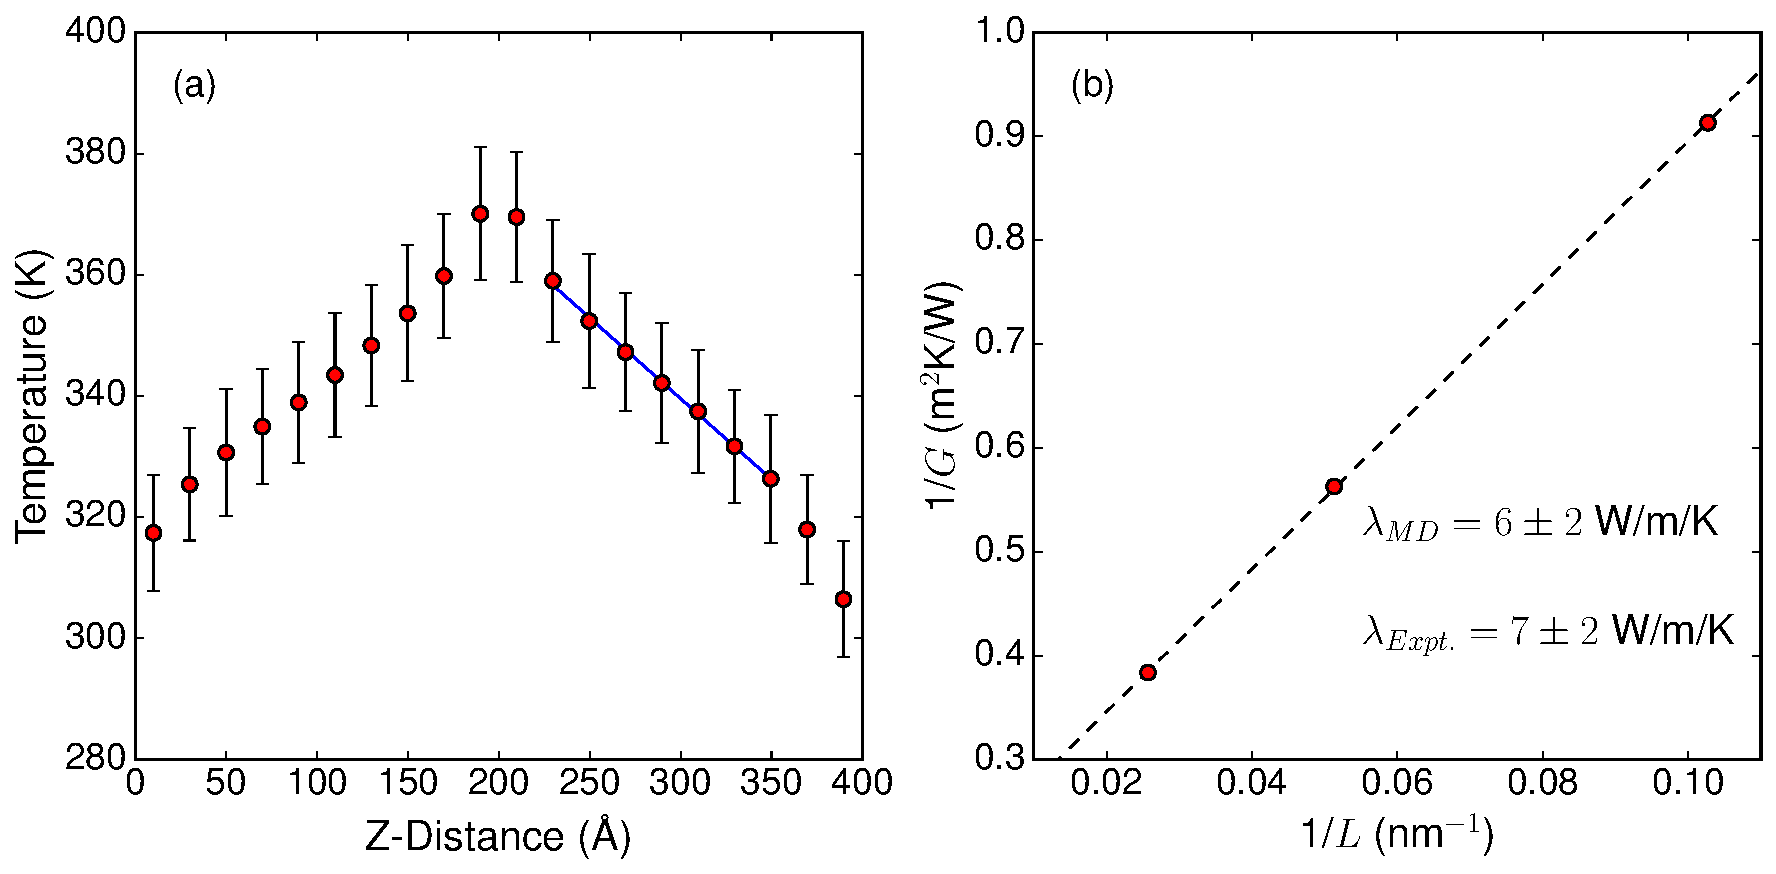
\includegraphics[width=\textwidth]{./Chapter4/rnemd1.pdf}
\caption[Determination of thermal conductivity in bulk CdSe via MD simulation.]{(a) Temperature profile along the kinetic energy exchange axis obtained following a 3 ns RNEMD simulation of a wurtzite CdSe slab. Error bars are derived from temperature deviations in each bin along the production trajectory. The solid blue line indicates a linear fit to the linear response region of the temperature profile. The slope of this line is used to obtain thermal conductivity via Eq. \ref{eq:rnemd1}.  (b) Inverse thermal conductivity (obtained as described above) as a function of inverse length. Extrapolation to the y-intercept yields the bulk (i.e., infinite length) thermal conductivity. Simulated ($\lambda_{MD}$) and experimental ($\lambda_{expt}$) values of thermal conductivity are given on the figure. Uncertainty values for $\lambda_{MD}$ were obtained from the average of four statistically independent RNEMD simulations, while the standard deviation in $\lambda_{expt}$ is obtained from an average of reported literature values \cite{berger1996semiconductor, PhysRevB.6.3791, doi:10.1021/nl400531f}.}
\label{f:rnemd1}
\end{center}
\end{figure}

To address the organic components of the system, our simulations utilize a combination of united-atom (UA) and explicit hydrogen (EH) parameters for the TraPPE force field \cite{doi:10.1021/jp0504827}.  The TraPPE model includes parametrizations for bonding interactions including stretches, bends, dihedrals, and torsions. For the amine terminal of the hexylamine molecules, TraPPE-EH parameters were used to model N and explicit H atoms to account for any role played by H in determining the packing of ligand monolayers on the CdSe surface. All other hydrocarbons utilized the TraPPE-UA model. Previous simulations of thermal conductivity which compared a similarly parametrized all-atom force field (the Optimized Potentials for Liquid Simulations - All Atom, or OPLS-AA \cite{jorgensen1988opls}) to the TraPPE-UA did not find a significant difference in the thermal conductivity obtained from RNEMD simulations between the two force fields. Thus, the TraPPE-UA models are computationally efficient while maintaining accuracy \cite{doi:10.1021/jp2073478}.  \par

\subsubsection{Simulation Protocol}

To construct CdSe surface/solvent interface models, a slab of crystalline (wurtzite) CdSe having a fixed cross-section of 30 \r{A}  $\times$ 30 \r{A} was built having a particular crystalline direction oriented along the z-axis of the simulation cell and then equilibrated at 200 K and 1 atm. For the systems studied here, 125 ps of equilibration time was found to be sufficient to ensure stable thermodynamic variables. Following equilibration in the NPT and NVT ensembles, the simulation cell was expanded along the z-axis to twice the length of the wurtzite slab. This empty space was filled with hexane molecules to experimental density at 200 K using the PackMOL algorithm \cite{JCC:JCC21224}.  The simulation cell was then equilibrated again at 200 K and 1 atm first in the NPT and then NVT ensemble. After all equilibration steps were complete, RNEMD simulations were run in the NVE ensemble using a target flux of 695 MW/m$^2$ and exchange time of 5 fs. RNEMD simulations were run for sufficiently long times to ensure the development of a stable temperature profile, typically 3 ns. \par

Passivated CdSe surfaces were constructed in a similar fashion. Hexylamine, a common experimental passivating ligand, was chosen for this study. Passivated CdSe surfaces were constructed by placing a hexylamine molecule, initially aligned along the z-axis of the simulation cell, atop each grafting site on the surface.  For the $11\bar{2}0$, $10\bar{1}0$, and $0001$ surfaces, hexylamine was initially placed top Cd atoms, while for the $000\bar{1}$ surface, which is Se terminated, hexylamine was placed atop Se atoms.  These placements are in agreement with DFT studies, which indicate that amine surface ligands primarily interact with surface Cd atoms \cite{doi:10.1021/jp064051f, doi:10.1021/jp903291d}.  After ligand placement, the system was equilibrated in an NVT ensemble to permit internal relaxation followed by equilibration at 200 K and 1 atm in the NPT ensemble. After these equilibration steps, the simulation cell was expanded to twice the length of the wurzite + ligand system and filled with hexane as before. The system was then equilibrated again at 200 K and 1 atm in the NPT and then NVT ensembles. Following these equilibration steps, RNEMD simulations were executed as described above. Ligand motion is unconstrained throughout the simulation; ligand molecules are free to sample the CdSe surface. Ligand migration occurs on the $000\bar{1}$ surface during equilibration, with ligand headgroups shifting to the interstitial sites in between surface Se atoms, situated roughly halfway between the surface Se atom and subsurface Cd atom below it. At the same time, these subsurface Cd atoms relax toward the surface. Ligand migration is minimal for the other surfaces studied here. All of the MD simulations in this work utilized the OpenMD software package \cite{gezelter2010openmd}.

\subsection{Results and Discussion}
Having established above that the Rabani interaction potential is well-suited for the simulation of thermal conductivity in bulk wurtzite CdSe, we now simulate the interfacial thermal conductance of various CdSe surfaces passivated and solvated by organic ligands.  Figure \ref{f:rnemd2}(a) details the chemically distinct components used to model solvent molecules in the simulations presented here.  The temperature profile resulting from a 3 ns RNEMD simulation of a CdSe($11\bar{2}0$)/hexane interface is shown in Figure \ref{f:rnemd2}(b).  Utilizing Eq. \ref{eq:rnemd2}, we obtain an interfacial thermal conductance of $\sim$8 MW/m$^2$/K for a 40 \r{A} long slab.  As with simulations of infinite, bulk materials, RNEMD simulations show convergence in the interfacial thermal conductance with respect to the size of the system. The dependence of $G$ on slab thickness arises from the disordering of atoms near the interface, resulting in an altered vibrational power spectrum with respect to the bulk atoms. In thin slabs, all atoms are close to an interface and therefore exhibit similar vibrational power spectra. This similarity yields higher $G$ values for thinner slabs. To isolate finite size effects from interfacial conductance, we performed RNEMD simulations on a series of slab lengths. The length of the hexane portion of the simulation cell was increased proportionally in each simulation. A fitting procedure similar to Eq. 5 \ref{eq:rnemd5} may be used to obtain $G$  values for a CdSe/hexane interface propagating to infinite length in the kinetic energy flux direction on either side of the interface.  Figure \ref{f:rnemd2}(c) displays the $G$ value obtained for 3 CdSe($11\bar{2}0$) slabs of increasing thickness.  The inset of Fig. \ref{f:rnemd2}(c) displays a snapshot of the CdSe($11\bar{2}0$)/hexane interface, taken from one of the trajectories used to produce the data.  Similar simulations were performed for the $10\bar{1}0$, $000\bar{1}$, and $0001$ surfaces.  These surfaces are of particular interest as they are the exposed surfaces of most CdSe nanocrystals \cite{doi:10.1021/nl0485861}.  Each of the surfaces yields a similar value for the interfacial thermal conductance (2 - 3.5 MW/m$^2$/K).  The results of our calculations for a bare CdSe/hexane interface are summarized in Table \ref{table:rnemdT1}. \par

\begin{figure}
\begin{center}
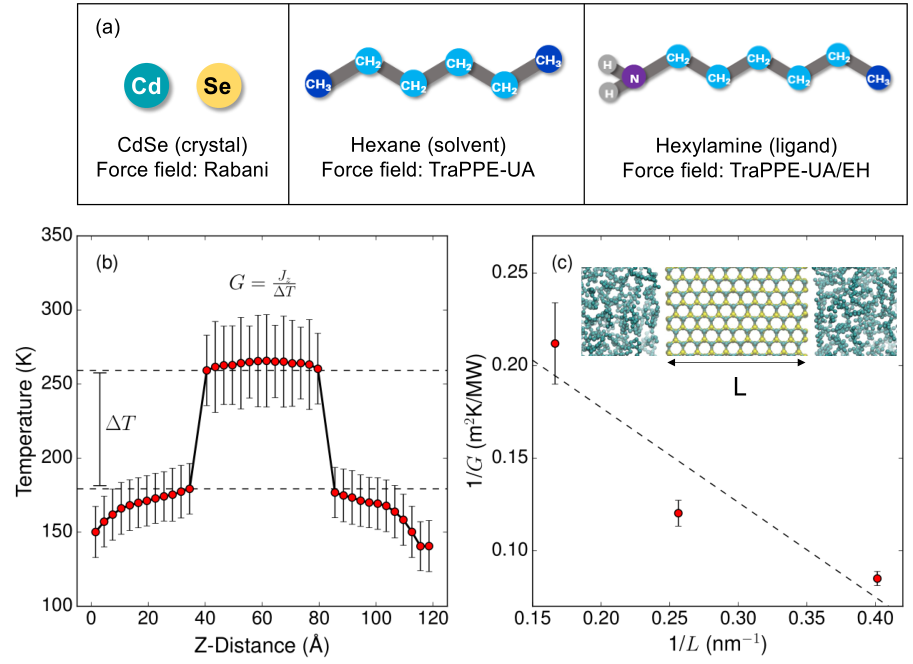
\includegraphics[width=\textwidth]{./Chapter4/rnemd2.png}
\caption[Details of RNEMD simulations of thermal transport at CdSe/hexane interfaces.]{ (a) Topologies of the molecules used in our simulations. The chemically distinct sites, given as colored spheres in the above diagram, are treated as united atoms. Amine headgroups are modeled with explicit hydrogen atoms \cite{doi:10.1021/jp0504827}. (b) Temperature profile along the kinetic energy exchange axis obtained for a system containing hexane and an unpassivated CdSe $11\bar{2}0$ slab. The discontinuities near 40 and 80 \r{A} represent the CdSe/hexane interface. The temperature drop at this interface, indicated by a dashed line in (a), is used to obtain the interfacial thermal conductance, $G$. Error bars are derived from temperature deviations in the bins along the production trajectory. (c) Inverse interfacial thermal conductance as a function of inverse slab length, $L$. As the length of the solvent region is also increased for larger simulations (fixed at $2L$), extrapolation to the y-intercept yields the interfacial thermal conductance for an infinitely thick slab of CdSe surrounded by an infinitely thick hexane bath. Inset: A snapshot from an MD trajectory used to produce this data. $L$ is indicated on the figure.}
\label{f:rnemd2}
\end{center}
\end{figure}

\begin{table}
\caption{RNEMD-Derived Interfacial Thermal Conductance Values for Four Surfaces of Wurtzite CdSe}
\centering
\begin{tabular}{l r}
\hline\hline
Surface & $G$ (MW/m$^2$/K) \\
\hline
$11\bar{2}0$ & 3.6 $\pm$ 0.9 \\
$10\bar{1}0$ & 1.7 $\pm$ 0.5 \\
$0001$ & 2.0 $\pm$ 0.6 \\
$000\bar{1}$ & 1.9 $\pm$ 0.6 \\
\hline
\end{tabular}
\label{table:rnemdT1}
\end{table}

Next, we probe the effects of surface passivation on the interfacial thermal conductance of the CdSe/hexane interface. Figure \ref{f:rnemd3} displays the temperature profile obtained for a completely passivated hexylamine-passivated $11\bar{2}0$ surface. Here, complete passivation is defined as having one hexylamine ligand for each surface atom, as described above. The temperature profile obtained here is more complicated owing to compositional heterogeneity and multiple interfaces. In this case, Eq. \ref{eq:rnemd3} is applied in the calculation of the interfacial thermal conductance. The interfacial thermal conductance values obtained for fully passivated hexylamine-passivated CdSe surfaces are summarized in Table \ref{table:rnemdT2}. To obtain average values of $G$, we performed four statistically independent RNEMD simulations of each surface. Statistical independence was ensured by generating initial velocity distributions from a different random seed for each replicated simulation. \par

\begin{figure}
\begin{center}
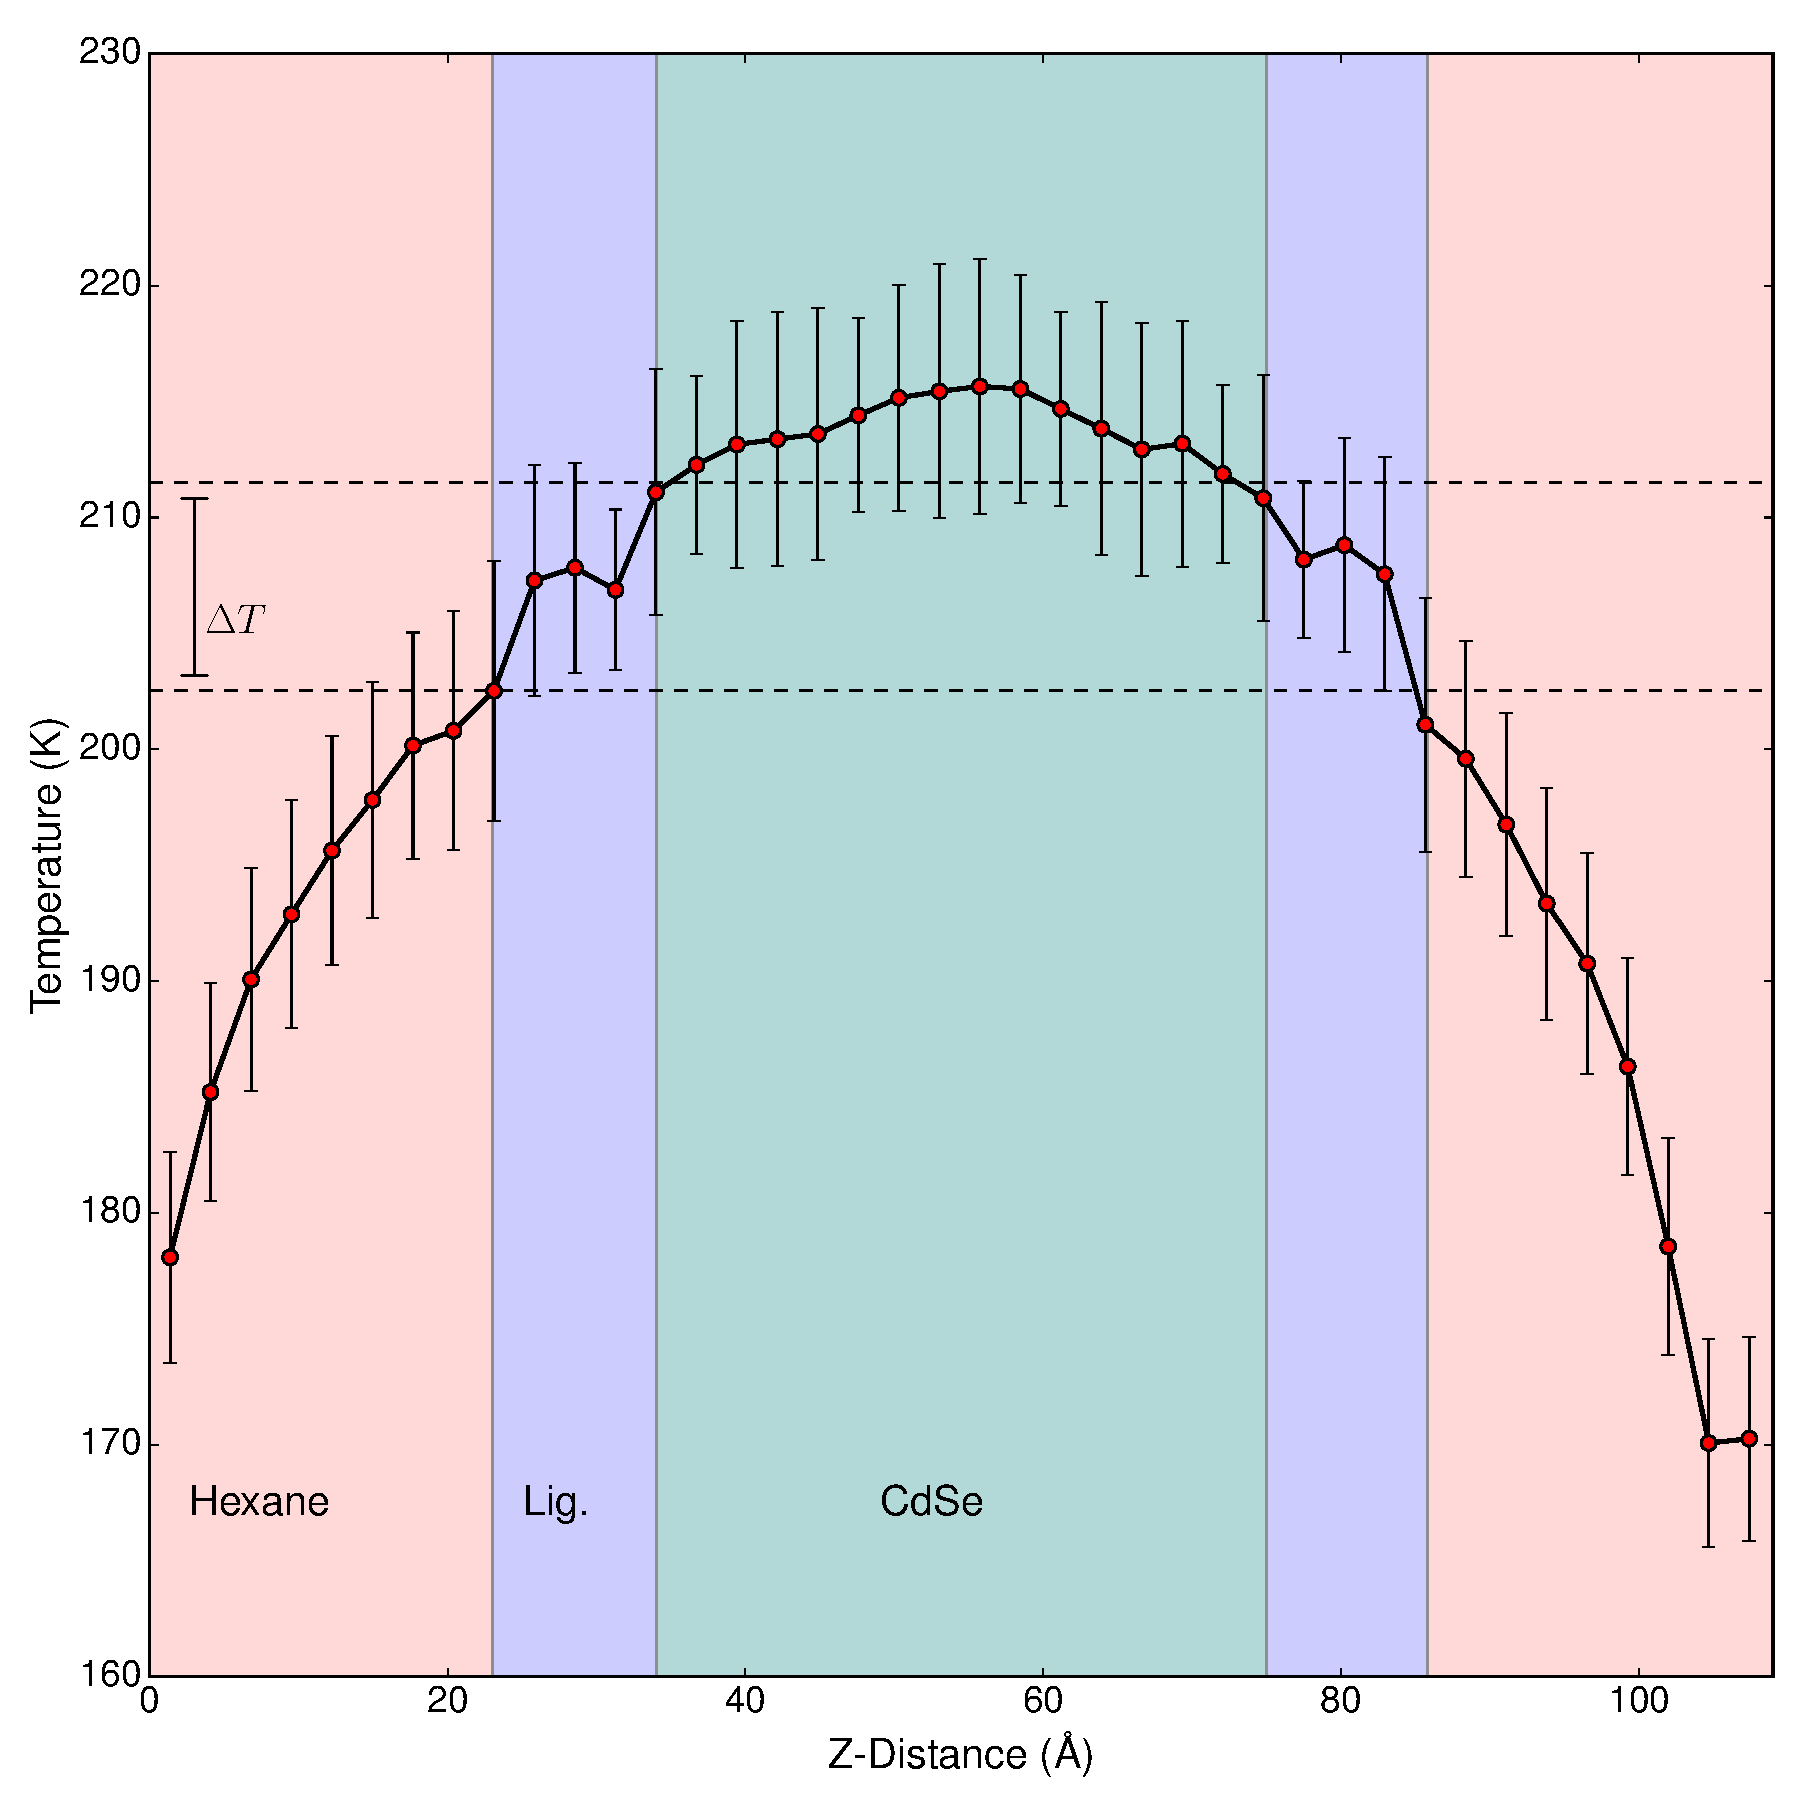
\includegraphics[width=\textwidth]{./Chapter4/rnemd3.pdf}
\caption[Temperature profile obtained from RNEMD simulation of CdSe/hexylamine/hexane interface.]{Temperature profile along the kinetic energy exchange axis obtained following a 3 ns RNEMD simulation of a system containing hexane (solvent) and a CdSe($11\bar{2}0$) slab passivated by hexylamine (ligand). The Z-coordinates corresponding to each region are labeled on the figure, with interfaces being designated by dashed lines. Error bars are derived from temperature deviations in the bins along the production trajectory.}
\label{f:rnemd3}
\end{center}
\end{figure}

\begin{table}
\caption{RNEMD-Derived Interfacial Thermal Conductance Values for Four Surfaces of Fully Passivated Wurtzite CdSe}
\centering
\begin{tabular}{l r}
\hline\hline
Surface & $G$ (MW/m$^2$/K) \\
\hline
$11\bar{2}0$ & 72 $\pm$ 12 \\
$10\bar{1}0$ & 80 $\pm$ 8 \\
$0001$ & 90 $\pm$ 7 \\
$000\bar{1}$ & 82 $\pm$ 11 \\
\hline
\end{tabular}
\label{table:rnemdT2}
\end{table}

As shown in Table 2, the presence of a passivating layer significantly increases the interfacial thermal conductance of a CdSe/hexane interface. This elevated thermal conductance can be understood in terms of improved vibrational overlap between CdSe and hexylamine as well as between hexane and hexylamine. Figure \ref{f:rnemd4}(a) displays the vibrational power spectrum of each distinct molecular component in the simulation cell (CdSe, hexylamine, hexane). The vibrational power spectrum is obtained by taking the Fourier transform of a velocity autocorrelation function obtained from 3 ns of simulation in an NVE ensemble subsequent to the pre-equilibration steps described above. This is shown in Equation \ref{eq:rnemd6}:
\begin{equation} \label{eq:rnemd6}
f(\omega) = \int^{+\infty}_{-\infty} \left\langle\vec{v}_A(t) \cdot \vec{v}_A(0)\right\rangle e^{-2\pi it\omega} dt
\end{equation}

\begin{figure}
\begin{center}
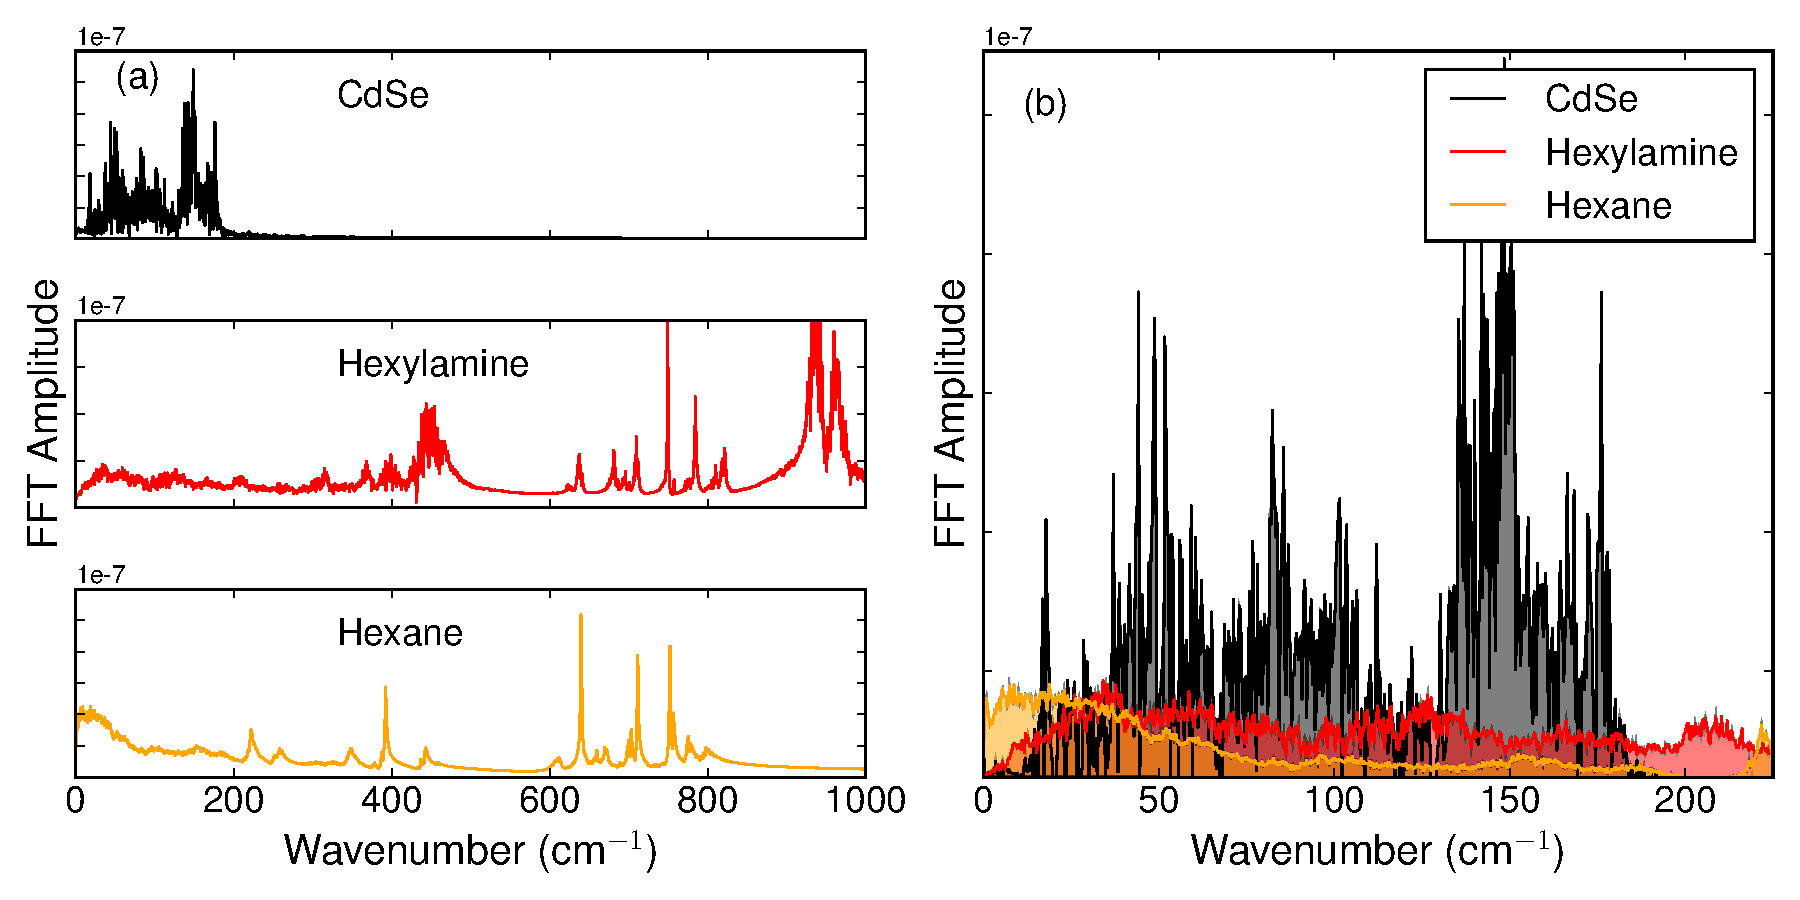
\includegraphics[width=\textwidth]{./Chapter4/rnemd4.pdf}
\caption[Vibrational power spectra for hexane, hexylamine, and CdSe.]{(a) Vibrational density of states at 200 K as obtained from Fourier transformation of the velocity autocorrelation function (eq 6) from an NVE simulation of a hexylamine-passivated, CdSe($11\bar{2}0$) surface surrounded by hexane. Each panel is labeled by molecular species. (b) Comparison of vibrational overlap at low frequencies. Hexylamine, shown in red, has a higher vibrational density of states than hexane (yellow) for most of this spectral region.}
\label{f:rnemd4}
\end{center}
\end{figure}

The hexylamine layer, shown in the middle of Figure \ref{f:rnemd4}(a), clearly exhibits greatly improved vibrational overlap with hexane, as these molecules are structurally and compositionally similar. Hexylamine also exhibits greater overall vibrational overlap with CdSe than hexane. This is emphasized in Figure \ref{f:rnemd4}(b), which focuses on the low frequency region containing the CdSe vibrational modes. \par

We also explore the dependence of interfacial thermal conductance on the extent of surface passivation. Figure \ref{f:rnemd5}(a) displays the interfacial thermal conductance as a function of ligand density on the surface, with each $G$ value (and its uncertainty) being the average (and standard deviation) of values obtained from four statistically independent RNEMD runs, as described above. Here, ligand density is defined as the number of hexylamine molecules in the simulation cell divided by the cross-sectional area of the CdSe slab. For the nonpolar $11\bar{2}0$ and $10\bar{1}0$ surfaces, $G$ increases roughly linearly with the extent of surface passivation. In contrast, the polar surfaces ($0001$ and $000\bar{1}$ show a nonmonotonic dependence of $G$ on the extent of surface passivation. Note, however, that the nonpolar $11\bar{2}0$ and $10\bar{1}0$ surfaces have a much lower atomic density and therefore do not support grafting densities as large as those supported by the polar surfaces. As indicated in \ref{f:rnemd5}(a), the highest ligand densities studied represent 100\% passivation of the surface, meaning that each surface site is interacting with a single passivating ligand. The polar CdSe surfaces have twice as many surface sites for a given cross-sectional area; this is demonstrated visually in Figure 5b, which highlights the number of surface sites for the $11\bar{2}0$, $10\bar{1}0$. and $0001$ surfaces. While no experimental estimate yet exists for the thermal conductance of CdSe/hexylamine/hexane interfaces, the $G$ values obtained here for maximal surface coverage are qualitatively similar to values experimentally measured for an oleate-passivated PbS nanocrystal array\cite{ong2013surface} and so are likely physically reasonable.

\begin{figure}
\begin{center}
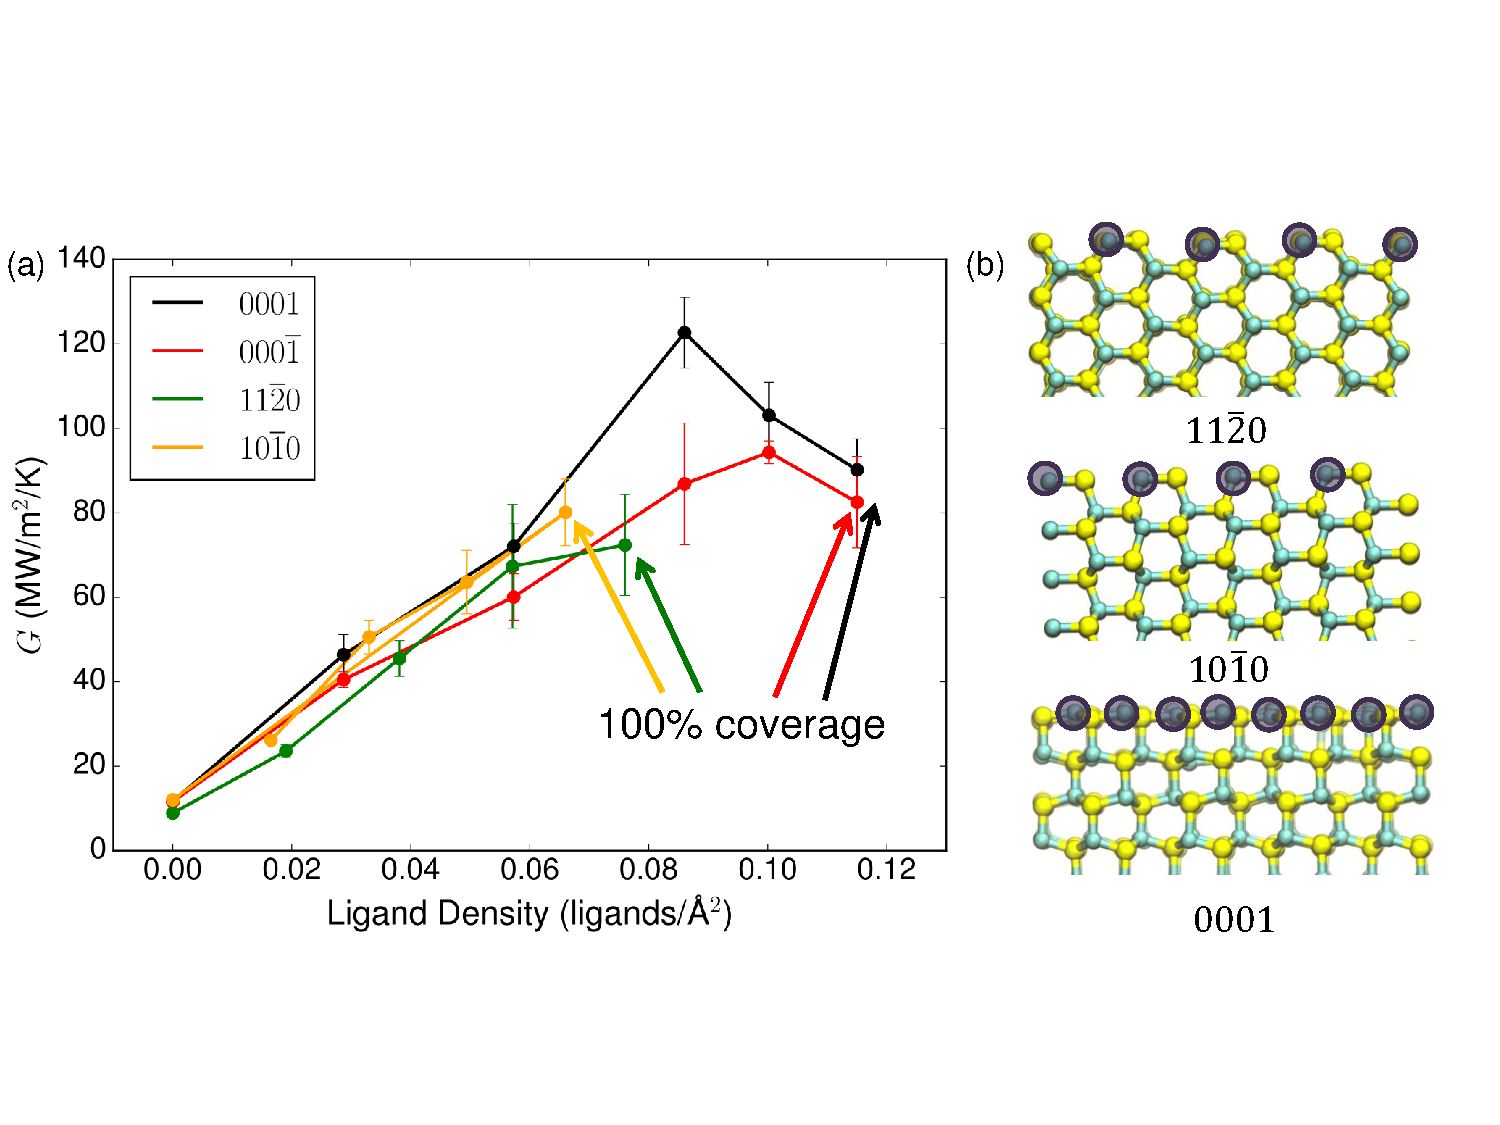
\includegraphics[width=\textwidth]{./Chapter4/rnemd5.pdf}
\caption[Dependence of interfacial thermal conductance on extent of surface passivation for a CdSe/hexylamine/hexane interface.]{(a) Vibrational density of states at 200 K as obtained from Fourier transformation of the velocity autocorrelation function (eq 6) from an NVE simulation of a hexylamine-passivated, CdSe($11\bar{2}0$) surface surrounded by hexane. Each panel is labeled by molecular species. (b) Comparison of vibrational overlap at low frequencies. Hexylamine, shown in red, has a higher vibrational density of states than hexane (yellow) for most of this spectral region.}
\label{f:rnemd5}
\end{center}
\end{figure}

The nonmonotonic dependence of $G$ on surface ligand density (Figure \ref{f:rnemd5}(a) can be understood as a balance of competing effects related to conduction, ordering, and excluded volume. First, surface ligands clearly facilitate heat conduction in the system via improved vibrational overlap (Figure \ref{f:rnemd4}). However, larger surface ligand densities also exclude solvent penetration into the ligand layer. Figure \ref{f:rnemd6} displays the time-averaged number density of both hexane (solvent) and hexylamine (ligand) along the kinetic energy exchange axis as obtained from analysis of RNEMD trajectories subsequent to the development of a stable temperature gradient. Density profiles for solvent and ligand resolved along the kinetic energy exchange axis can be found in Appendix E for all of the surfaces and ligand coverages examined in this Chapter. Higher ligand coverages clearly coincide with reduced solvent penetration into the same region; density profiles for each coverage can be found in Appendix E. Ligand and solvent molecules have a roughly equal number density at $\sim$35\% ligand coverage, which should maximize conduction effects, as every hexane molecule in the ligand layer, at least in principle, has a hexylamine partner available for coupling. This first-order analysis, however, ignores effects due to orientational ordering and solvent trapping in the ligand layer. \par

\begin{figure}
\begin{center}
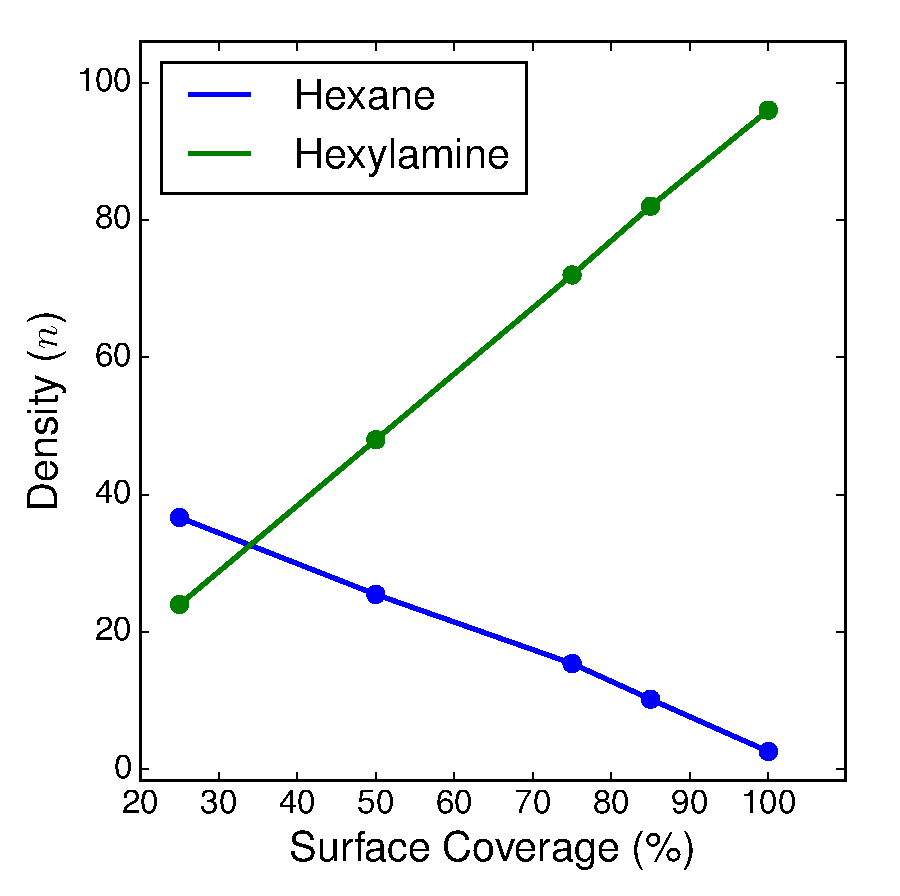
\includegraphics[width=0.5\textwidth]{./Chapter4/rnemd6.pdf}
\caption[Number density of hexane and hexylamine molecules in the hexylamine layer as a function of surface coverage.]{Integrated number density in the ligand region for ligand (hexylamine) and solvent (hexane) molecules as a function of surface coverage on a $0001$/$000\bar{1}$ CdSe slab. These curves intersect at roughly 35\% surface coverage.}
\label{f:rnemd6}
\end{center}
\end{figure}

While low ligand coverage permits greater solvent penetration into the ligand layer, these solvent molecules are less likely to be ordered in a fashion conducive to thermal energy transfer. As molecular alignment plays an important role in facilitating thermal energy transfer \cite{shen2010polyethylene}, the relative orientation of ligand molecules and solvent molecules in the ligand layer must be considered. Qualitatively, it is expected that higher ligand densities will force interpenetrating solvent molecules into alignment. This effect can be examined via diagonalization of an order parameter tensor given by Eq. \ref{eq:rnemd7}: \par
\begin{equation} \label{eq:rnemd7}
Q_{\alpha\beta} = \frac{1}{2N}\sum^N_{i = 1} \left(3\vec{e}_{i\alpha}\vec{e}_{i\beta} - \delta_{\alpha\beta}\right)
\end{equation}
In Eq. \ref{eq:rnemd7}, $\vec{e}_{i\alpha}$ is the $\alpha = x, y, z$ component of the unit vector $\vec{e}_i$, defined here as a vector along the terminal atoms of a given solvent or ligand molecule. The summation runs over all of the molecules being considered, with $N$ representing the total number of molecules of a particular type (solvent or ligand). The Kroenecker delta function is represented by $\delta_{\alpha\beta}$. The largest eigenvalue of $Q$ is traditionally used to obtain the orientational order parameter, while the eigenvector associated with that eigenvalue is the director axis, $\vec{d}(t)$. The director axis defines the average direction of molecular alignment at time $t$. The alignment of ligand molecules and entrapped solvent molecules can be quantified as the time-averaged dot product of the director axes of each respective molecule, as shown in Eq. \ref{eq:rnemd8}: 
\begin{equation} \label{eq:rnemd8}
\left\langle d \right\rangle = \left\langle \vec{d}_{hexylamine}(t) \cdot \vec{d}_{hexane}(t)\right\rangle
\end{equation}
This quantity ranges between 0 (hexane and hexylamine molecules aligned perpendicularly) and 1 (parallel alignment). This dot product is displayed as a function of ligand surface coverage in Figure \ref{f:rnemd7}(a) for a CdSe $0001$/$000\bar{1}$ surface. Generally $\left\langle d \right\rangle$ is larger for higher surface coverages, reflecting the formation of “pockets” which force interpenetrating solvent molecules into alignment \cite{doi:10.1021/jp312734f}. The anomalously low value of $\left\langle d \right\rangle$ for 100\% surface coverage reflects the near-complete exclusion of solvent from the ligand layer (Figure \ref{f:rnemd6}(e)). This alignment facilitates efficient thermal coupling, offsetting the decreased penetration of solvent into the ligand layer. \par

\begin{figure}
\begin{center}
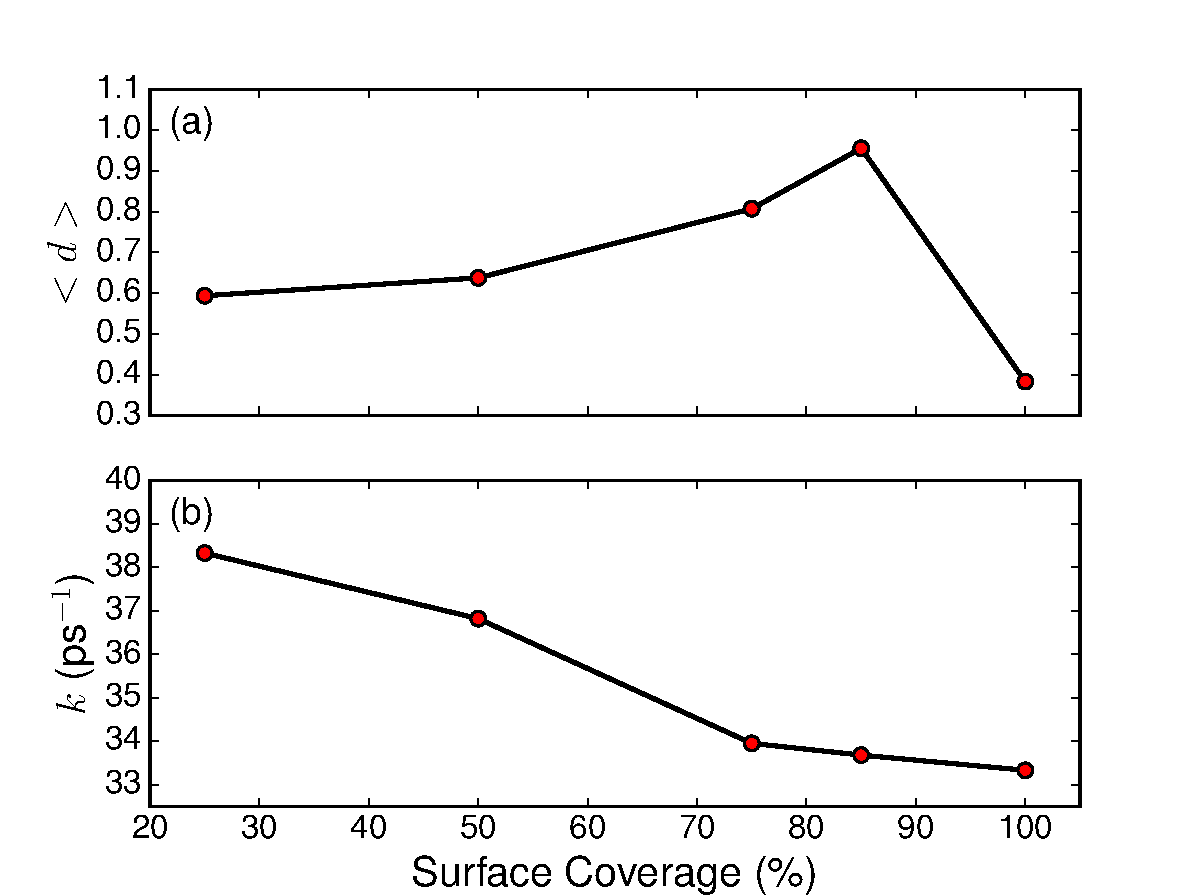
\includegraphics[width=0.75\textwidth]{./Chapter4/rnemd7.pdf}
\caption[Alignment and time-averaged residence time of solvent molecules in a passivating ligand layer on a CdSe surface.]{(a) Time-averaged dot product of the director axis for hexylamine molecules and hexane molecules present in the hexylamine layer, as defined in Eq. \ref{eq:rnemd8}, as a function of surface coverage for the $0001$/$000\bar{1}$ surfaces. (b) Solvent escape rate, $k$, as a function of surface coverage for the $0001$/$000\bar{1}$ CdSe surfaces.}
\label{f:rnemd7}
\end{center}
\end{figure}

In addition to the average density of solvent molecules in the ligand layer, the time scales of solvent movement into and out of the ligand layer are also of interest. To analyze these time scales, we utilize a survival correlation function which measures the residence time of a solvent molecule in the ligand layer. This function, $C(t)$, correlates the identity of all hexane molecules within the ligand layer at two times. If the solvent molecule is present at both times, the configuration contributes a 1, and contributes a 0 otherwise. A 0 contribution indicates that the solvent molecule has migrated back into the bulk liquid, and so a steep decay of $C(t)$ indicates a high turnover rate of solvent molecules in the ligand region. We define this solvent escape rate, $k$, for a simulation of duration $T$, according to Eq. \ref{eq:rnemd9}: 
\begin{equation} \label{eq:rnemd9}
k = \left(\int^T_0 C(t)dt)\right)^{-1}
\end{equation}
Figure \ref{f:rnemd7}(b) $k$ as a function of surface coverage. As surface ligand density increases, $k$ decreases, indicating that solvent molecules spend a longer time trapped in the ligand layer at high coverages. Depending on the time scale of heat transfer between the hexylamine ligands and hexane molecules in the ligand layer, the increased residence time of the solvent molecules at higher coverages my facilitate thermal transport by allowing the solvent molecules adequate time to thermalize with the ligands before returning to the bulk liquid. While $G$ does decrease for surface coverages yielding the lowest $k$ values, it is unlikely that the residence time of solvent molecules in the ligand layer is long enough to impede interfacial thermal conductance. Given the extremely small relative change in k ($\sim$2) over the 75-100\% surface coverage range, the decrease in $G$ is more likely a result of solvent exclusion (Figure \ref{f:rnemd6}), which eventually overwhelms positive contributions to interfacial thermal conductance due to orientational ordering and vibrational overlap. It is the interplay of these effects which ultimately yields the nonmonotonic dependence of $G$ on surface coverage for the polar CdSe surfaces (Figure \ref{f:rnemd5}(a)).

\subsection{Conclusion}
Our results highlight the important role played by surface chemistry and crystal structure in mediating thermal transport across chemically passivated semiconductor interfaces. Generally, passivation of a CdSe surface with hexylamine increases the thermal conductance of the interface by more than 1 order of magnitude. Furthermore, we find that while $G$ increases with increasing surface coverage at lower ligand-grafting densities, $G$ decreases at the highest grafting densities. \par

The nonmonotonic dependence of $G$ on surface coverage is a manifestation of several competing phenomena. Hexylamine (the passivating ligand) exhibits improved vibrational overlap with both CdSe and hexane (the solvent). The presence of hexylamine thus facilitates efficient thermal coupling in the system. However, as ligand grafting on the surface becomes increasingly dense, exclusion of solvent molecules from the ligand layer occurs. At the same time, higher ligand coverage tends to force into alignment any solvent molecules which do manage to penetrate into the ligand layer, yielding more efficient vibrational coupling of these molecules. Higher coverages also result in decreased solvent escape rates, though these decreases are unlikely to play a dominant role in determining $G$. Taken in aggregate, these effects produce maximal interfacial thermal conductance at ligand-grafting density values in the range of 0.08-0.1 ligands/\r{A}$^2$. These grafting density values represent a fractional coverage that varies for a particular facet. For the nonpolar surfaces ($10\bar{1}0$, and $11\bar{2}0$), a ligand-grafting density of 0.08 represents a full monolayer (all binding sites occupied), while the same grafting density represents roughly 75\% of a monolayer for the polar surfaces ($0001$ and $000\bar{1}$). The ligand-grafting density corresponding to a full monolayer (100\% coverage) for each surface is indicated in Figure \ref{f:rnemd5}(a). \par

While the interfacial thermal conductance of bare CdSe surfaces was found to be similar for each of the surfaces studied, crystal structure nevertheless plays an extremely important role, as the number of available binding sites on each surface ultimately determines the limit of ligand-grafting density. For example, for the wurtzite crystal structure, passivated nonpolar surfaces exhibit much lower interfacial thermal conductance than passivated polar surfaces owing to fewer binding sites per unit area of the nonpolar surface. As synthetic methods for semiconductor nanocrystals have become increasingly sophisticated, particularly for metal chalcogenide nanocrystals, chemical control of the surface areas of each facet has become a possibility. Our results therefore have interesting implications for the synthetic manipulation of interfacial thermal conductance in this technologically important material class. \par

The specific case of a crystalline CdSe semiconductor material was examined in this work, but the phenomena identified are general. The dependence of ligand-grafting density (and, thus, interfacial thermal conductance) on the particular exposed surface is a previously unreported phenomenon; prior studies examining gold surfaces find that ligand-grafting density is primarily determined by the steric behavior of the ligands. This effect likely stems from the fact that CdSe is a binary compound and only half of the exposed atoms on a nonpolar surface will interact strongly with ligands, resulting in lower overall grafting density for these surfaces. The hexagonal lattice and different structural parameters of CdSe as compared to Au may also play a role. Regardless, our results highlight for the first time the possibility of atomic structure on the exposed crystal surface being the primary factor in determining the interfacial thermal conductance of chemically passivated interfaces. In the limit that interfacial thermal conductivity dictates the overall thermal transport rate involving a semiconductor, variation in the surface termination and exposed surface area offers a route to anisotropic transport that can aid thermoelectric efficiencies or improve heat dissipation from LEDs, lasers, and solar cells.

\chapter{Engineering Thermal Processes in Semiconductor Nanocrystals}

Work in this Chapter is adapted from the following papers:
\begin{itemize}
\item Hannah, D.C.; Ithurria, S.; Krylova, G.; Talapin, D.V.; Schatz, G.C.; Schaller, R.D. \emph{Nano Letters} \textbf{2012} 12, 5797
\end{itemize}

Theoretical work in this Chapter is adapted, in part, from the following papers:

\begin{itemize}
\item Rowland, C.E.; Liu, W.; Hannah, D.C.; Chan, M.K.Y.; Talapin, D.V.; Schaller, R.D. \emph{ACS Nano} \textbf{2013}, 8, 977
\item Rowland, C.E.; Hannah, D.C.; Demortiere, A.; Yang, J.; Cook, R.E.; Prakapenka, V.B.; Kortshagen, U.R.; Schaller, R.D. \emph{ACS Nano} \textbf{2014}, 8, 9219
\end{itemize}

\section{Overview}

While much research involving NCs examines optical and electrical processes such as charge separation and transport, phonon transport is equally critical to many device applications. Specifically, thermoelectrics benefit from minimal phonon transport as power conversion efficiency relates inversely to thermal conductivity \cite{doi:10.1021/cm902195j} whereas optical sources such as LEDs and lasers \cite{doi:10.1021/nl9002969,Klimov13102000} require maximal transport where high thermal conductivity improves brightness at high currents and extends operational longevity \cite{Narendran2004449}.  Spatially periodic arrays of scattering centers have been demonstrated as a top-down means to manipulate phonon transport \cite{cheng2006observation,PhysRevLett.94.115501,doi:10.1021/nl102918q,PhysRevLett.100.194301}, but this scheme presents inherent problems for many applications since it necessitates higher-order material organization. Rather, component-level, bottom-up engineering of phonon transport via direct tuning of the NC thermal properties imposes fewer requirements on the overall structure, which in some cases may comprise only a single active NC layer \cite{doi:10.1021/nl9002969}. Ideally, for a given application, one would like to separately select the semiconductor component energy gap as well as the material thermal conductivity for optimal device operation. \par

In this Chapter, we demonstrate using a combination of experimental characterization and theoretical modeling that appropriate modification of semiconductor nanocrystal surfaces can manipulate thermal transport rates independently of optical properties and improve the thermal stability of semiconductor NC materials at the single particle level.

\section{Particle-Level Engineering of Thermal Conductivity in Matrix-Embedded Semiconductor Nanocrystals}

As detailed in Chapter 3, non-contact characterization of thermal transport from NCs has been achieved by monitoring optical signatures of phonon outflow arising from transient phonon-assisted radiative recombination from the lowest-energy exciton fine structure state (the “dark” exciton state), for which transitions are ordinarily dipole-forbidden. As schematically described in Figure \ref{f:plevel1}(a) for a NC initially at a very low temperature (3 K), ultrafast intraband relaxation of excited charge carriers produces dark-excitons and nonequilibrium phonons typically within $\sim$1 ps following excitation. Acoustic phonons in particular impart distortions of the NCs that transiently perturb exciton fine structure and assist in angular momentum conserving radiative transitions \cite{:/content/aip/journal/jcp/132/10/10.1063/1.3350871,doi:10.1021/jp201408m}. As a result, rapid phonon-mediated radiative recombination occurs with a higher photon generation rate during the period of time in which the NC contains acoustic phonons, than in unperturbed NCs containing a dark exciton (Figure \ref{f:plevel1}(b)).  As time progresses, these phonons flow out from NCs into the surrounding matrix on a time scale consistent with diffusion-limited thermal transport. Following the outflow of acoustic phonons, radiative recombination occurs via concurrent emission of a photon and a 25-meV longitudinal optical (LO) phonon, which gives rise to a NC-size independent spectral red-shift between early- and late-time emission spectra (Figure \ref{f:plevel1}(c)). Despite the early-to-late PL energy shift, spectral linewidths over this time range remain constant, consistent with a single population evolving in time to emit at a lower energy. The slower radiative rate of the late-time LO-phonon-assisted recombination process results in fewer detected photons per unit time subsequent to the outflow of acoustic phonons. The initial spike in emission intensity is only apparent at low temperatures (though we expect the physics presented is relevant for higher temperatures), since at high sample temperatures (near 80 K) an equilibrium population of acoustic phonons in NCs exists that does not decay to zero with time. That is, the perturbation from acoustic phonons persists continuously at higher temperatures \cite{PhysRevLett.107.177403}.

\begin{figure}
\begin{center}
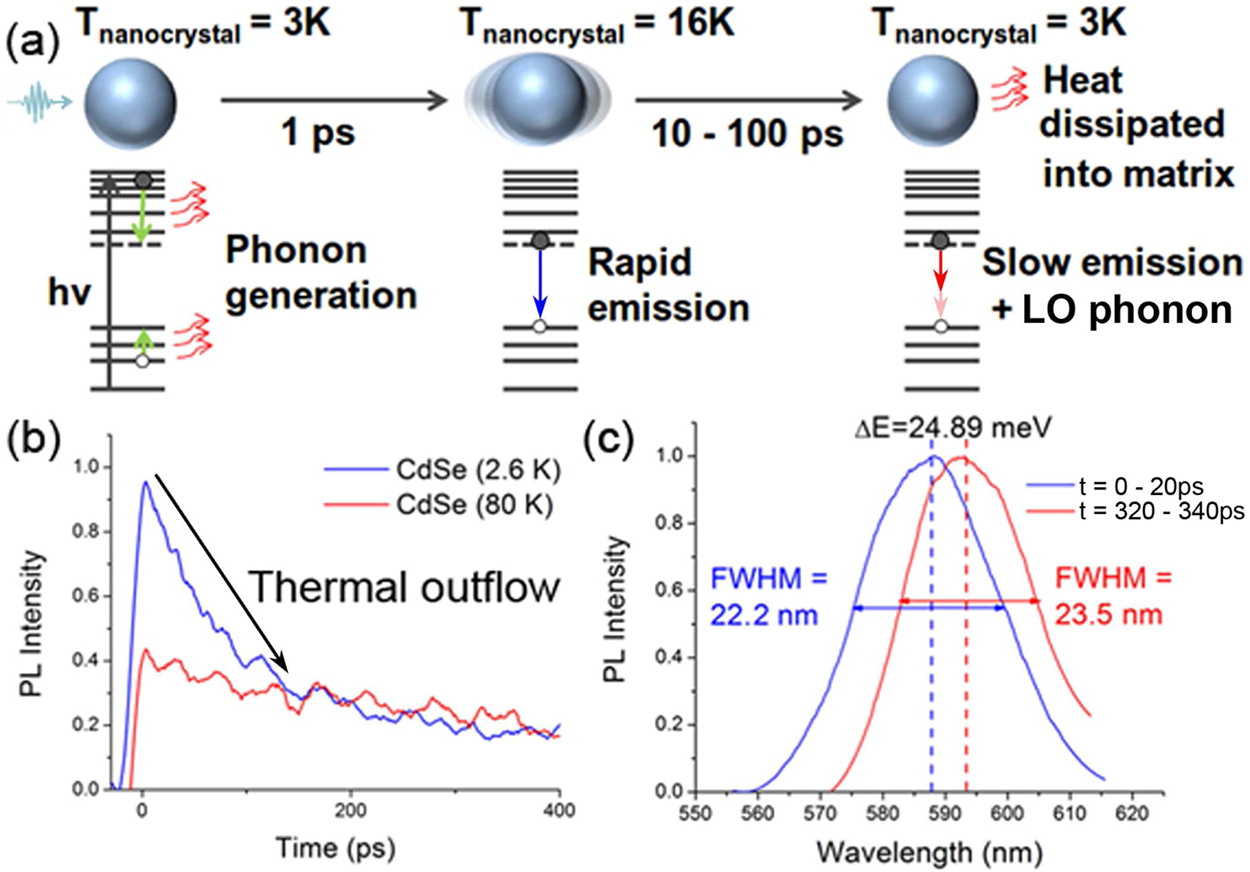
\includegraphics[width=0.75\textwidth]{./Chapter5/plevel1.jpeg}
\caption[Synopsis of thermal outflow detection in CdSe NCs.]{Synopsis of thermal outflow detection in CdSe NCs. (a) A photoexcited NC at low temperature (3 K) undergoes intraband relaxation on a $\sim$1 ps time scale, resulting in the population of lattice vibrations and dark excitons. Subsequent to thermalization with the surrounding matrix, radiative recombination of dark excitons occurs via a LO-phonon assisted mechanism, resulting in microsecond radiative lifetimes. (b) Dynamics for a 3.8-nm diameter CdSe NC are shown at 3 and 80 K; biexponential dynamics are observed at 3 K. The rapid emission feature corresponding to thermal outflow from NCs is indicated. (c) Representative time-resolved emission spectra for matrix-embedded CdSe NCs at 3 K. The 25-meV red-shift with increasing time is consistent with initial acoustic phonon assisted PL followed by 25-meV LO-phonon assisted PL, while the consistent line width (indicated) suggests a single population evolves in time.}
\label{f:plevel1}
\end{center}
\end{figure}

Here, using the above-described transient PL (trPL) technique, we report measurements of heat transport time scales for matrix-embedded semiconductor NCs with the goal of manipulating thermal outflow times. Upon growing an electronically noninteracting ZnS shell of controlled thickness, we show that the phonon outflow time increases significantly. In particular, we find that the fitted lifetime of the exponential decay related to phonon transport increases with increasing ZnS shell thickness for a fixed CdSe NC core size. We also measure numerous core-shell samples comprising different core sizes and determine that the phonon outflow time follows the overall particle size. These findings shows that phonon outflow times can be tuned separately from the optical energy gap via manipulation of the overall particle size at the component level. \par

Near-spherically shaped CdSe NCs were synthesized using a previously described seeded-growth approach \cite{doi:10.1021/nl0717661}.  ZnS shell-growth also followed a previously described procedure, summarized here \cite{doi:10.1021/nl0155126}. A solution of as-synthesized CdSe NCs was heated and mixed with trioctylphosphine oxide and hexadecylamine. A Zn:S stock solution was added dropwise to the CdSe NC solution and stirred vigorously. The amount of stock solution necessary to obtain a desired shell thickness was calculated from the ratio between core and shell volumes using bulk lattice parameters of CdSe and ZnS. Samples were characterized by optical absorption and emission as well as transmission electron microscopy (TEM). For optical experiments, NCs were dissolved in molten octadecane and drop cast onto a sapphire disk. The volume fraction of NCs was <1\% for all presented experiments. Samples were loaded into a closed-cycle helium cryostat and excited with 35-fs pump pulses at 2 kHz with 3-eV photon energy. To ensure single-exciton dynamics, pump fluence was adjusted such that the average number of excitons per NC was less than 1. Four times higher or lower fluence did not alter observed dynamics (see Appendix A). \par

\begin{figure}
\begin{center}
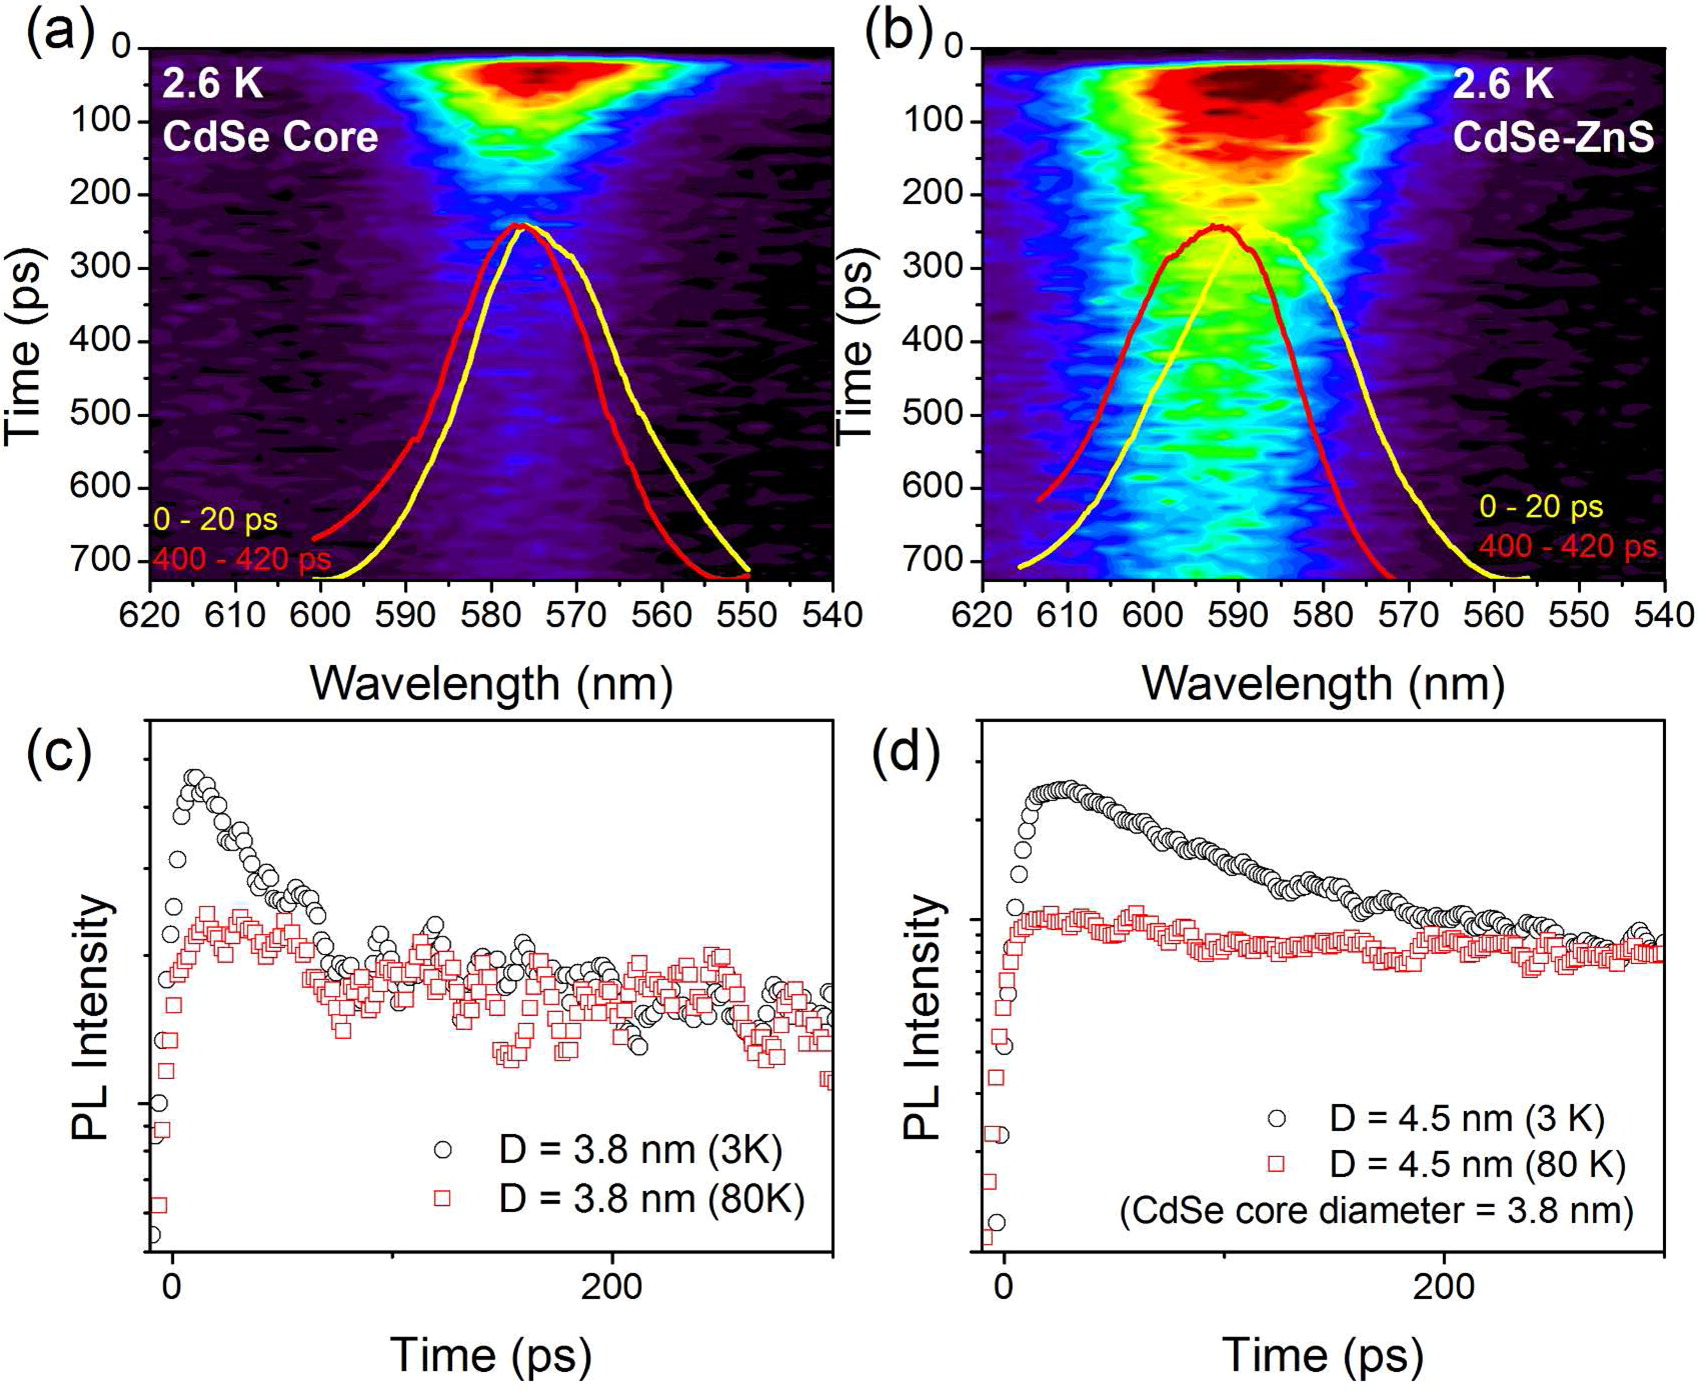
\includegraphics[width=0.75\textwidth]{./Chapter5/plevel2.jpeg}
\caption[Comparison of PL decay dynamics between core-only and core-shell CdSe NCs.]{(a) A streak camera image for a 3.8-nm diameter core-only CdSe NC photoexcited at 3 eV. The spectral overlays show time-integrated emission from $t = 0 - 20$ ps (yellow) and $t = 400 - 420 ps$ (red). (b) The same for a 4.5-nm diameter CdSe-ZnS core-shell NC with the same 3.8-nm diameter CdSe core as in panel a. (c) Comparison of PL dynamics at 2.6 K (black circles) and 80 K (red squares) for the 3.8-nm CdSe core-only sample and (d) for the 4.5-nm CdSe-ZnS core-shell sample. Note the longer time scale of the low-temperature decay feature in d.}
\label{f:plevel2}
\end{center}
\end{figure}

Figure \ref{f:plevel2}(a) and (b) shows subnanosecond streak-camera images of trPL recorded at 2.6 K for a 3.8-nm diameter ($D$) CdSe NC core (Figure \ref{f:plevel2}(a) and the same core size overcoated with a wide-gap ZnS shell to yield a 4.5-nm CdSe-ZnS core-shell particle (Figure \ref{f:plevel2}(b)). We display time-resolved spectra integrated for $t = 0-20$ ps (early) and $t = 400-420$ ps (late) superimposed on the streak camera images. A clear 25-meV red-shift from early to late time, which appears for all samples examined, matches the LO-phonon energy of bulk CdSe (see above). Figure \ref{f:plevel2}(c) and d shows dynamics for both a core-only and a core-shell NC sample that have been spectrally binned for wavelengths to the blue of the late-time PL band center (“blue-side” dynamics), which emphasizes the fast decay component. Both samples clearly exhibit an initial subnanosecond decay component at 2.6 K that is not observed at 80 K (as shown in Figure \ref{f:plevel2}(c) and (d)). Notably the fast feature decay lifetime becomes significantly longer for the core-shell sample. The elevation of the sample temperature to 80 K causes a loss of the fast feature amplitude relative to the late-time amplitude, which we previously showed for CdSe core-only NCs was consistent with Boltzmann thermal partitioning \cite{PhysRevLett.107.177403} with acoustic phonon energies spanning 0.8-1.8 meV. As rapid emission appears acoustic-phonon mediated, the difference in lifetime between the core and the core-shell samples (Figure \ref{f:plevel2}(c) and (d)) suggests that acoustic phonon dissipation times might be controlled via the overall particle size. \par

To begin with, the elastic constants of CdSe and ZnS are similar ($\rho_{CdSe} = 5816$ g/m$^3$, $\rho_{ZnS} = 4075$ g/m$^3$, $v_{sound, CdSe} = 3559$ m/s, $v_{sound, ZnS} = 3868$ m/s), which suggests a small acoustic impendence mismatch at the CdSe-ZnS interface, in comparison to the semiconductor-to-organic interface. Grossly approximating as a planar interface, calculations based on the acoustic mismatch model for the CdSe-to-ZnS interface yield a phonon transmission coefficient of 0.99, whereas the ZnS-to-organic interface yields nearly an order of magnitude lower value of only 0.15. As a result, heat deposited in the CdSe core due to intraband relaxation likely distributes rapidly throughout the entire core-shell structure. Previously we showed that thermalization of a NC lattice with its environment closely followed diffusion-limited times for thermal outflow \cite{PhysRevLett.107.177403}. Diffusion-limited thermal outflow time depends proportionately on the surface area of the NC in contact with the matrix. Therefore, we attempted to modify particle thermalization rates for CdSe-ZnS core-shell NCs by manipulating the overall particle size. \par  

Figure \ref{f:plevel3} relates the dependence of total particle size on thermal outflow time. Here, we subtract the slow emission component observed at long times from early PL amplitude to emphasize the early time exponentially decaying component. Figure \ref{f:plevel3}(a) depicts PL dynamics for a series of CdSe core-only samples of increasing size. Lifetimes increase for larger CdSe NC radii, where the smallest sample exhibits a thermal outflow lifetime of 10.3 ps and the largest core-only sample presents a lifetime of 106.7 ps. Figure \ref{f:plevel3}(b) presents data for samples wherein overall particle size increases via the growth of a progressively thicker ZnS shell on a fixed-size CdSe core. For this fixed, intermediate-sized CdSe core, the rapid-emission lifetime increases from 25.9 ps in the smallest core-shell NC to 130.3 ps in the largest core-shell NC. The relationship between overall particle size (including core and shell) and thermal outflow lifetime for various CdSe core-only NCs and random shell-thickness CdSe-ZnS NCs is plotted in Figure \ref{f:plevel3}(c). This comparison illustrates that overall particle size heavily dictates phonon outflow time. Figure \ref{f:plevel3}(d) displays thermal outflow times for a series CdSe cores of increasing size as well as for a series of fixed-size CdSe cores with a ZnS shell of increasing thickness. From this comparison, it is apparent that thermal outflow time can be tuned largely independently of the emission energy, which is dictated by the core size. Specifically, in the case of core-only samples, emission energies ranging from blue-green (2.6 eV) to red (1.9 eV), a shift of 700 meV, yield thermal outflow times that differ by roughly a factor of 9. On the other hand, thermal outflow times from the smallest to largest CdSe-ZnS (with a fixed core size) sample differ by a factor of 5 with a commensurate emission energy shift of only 90 meV. Thus, shell thickness manipulation demonstrates two points. First, shell thickness manipulation can separate the nominal codependence of the energy gap from thermal outflow time. Second, the demonstrated manipulation of the fast decay dynamics using a nonelectronically interacting shell further supports the notion that the observed dynamics are extrinsic in relation to properties of the core. \par

\begin{figure}
\begin{center}
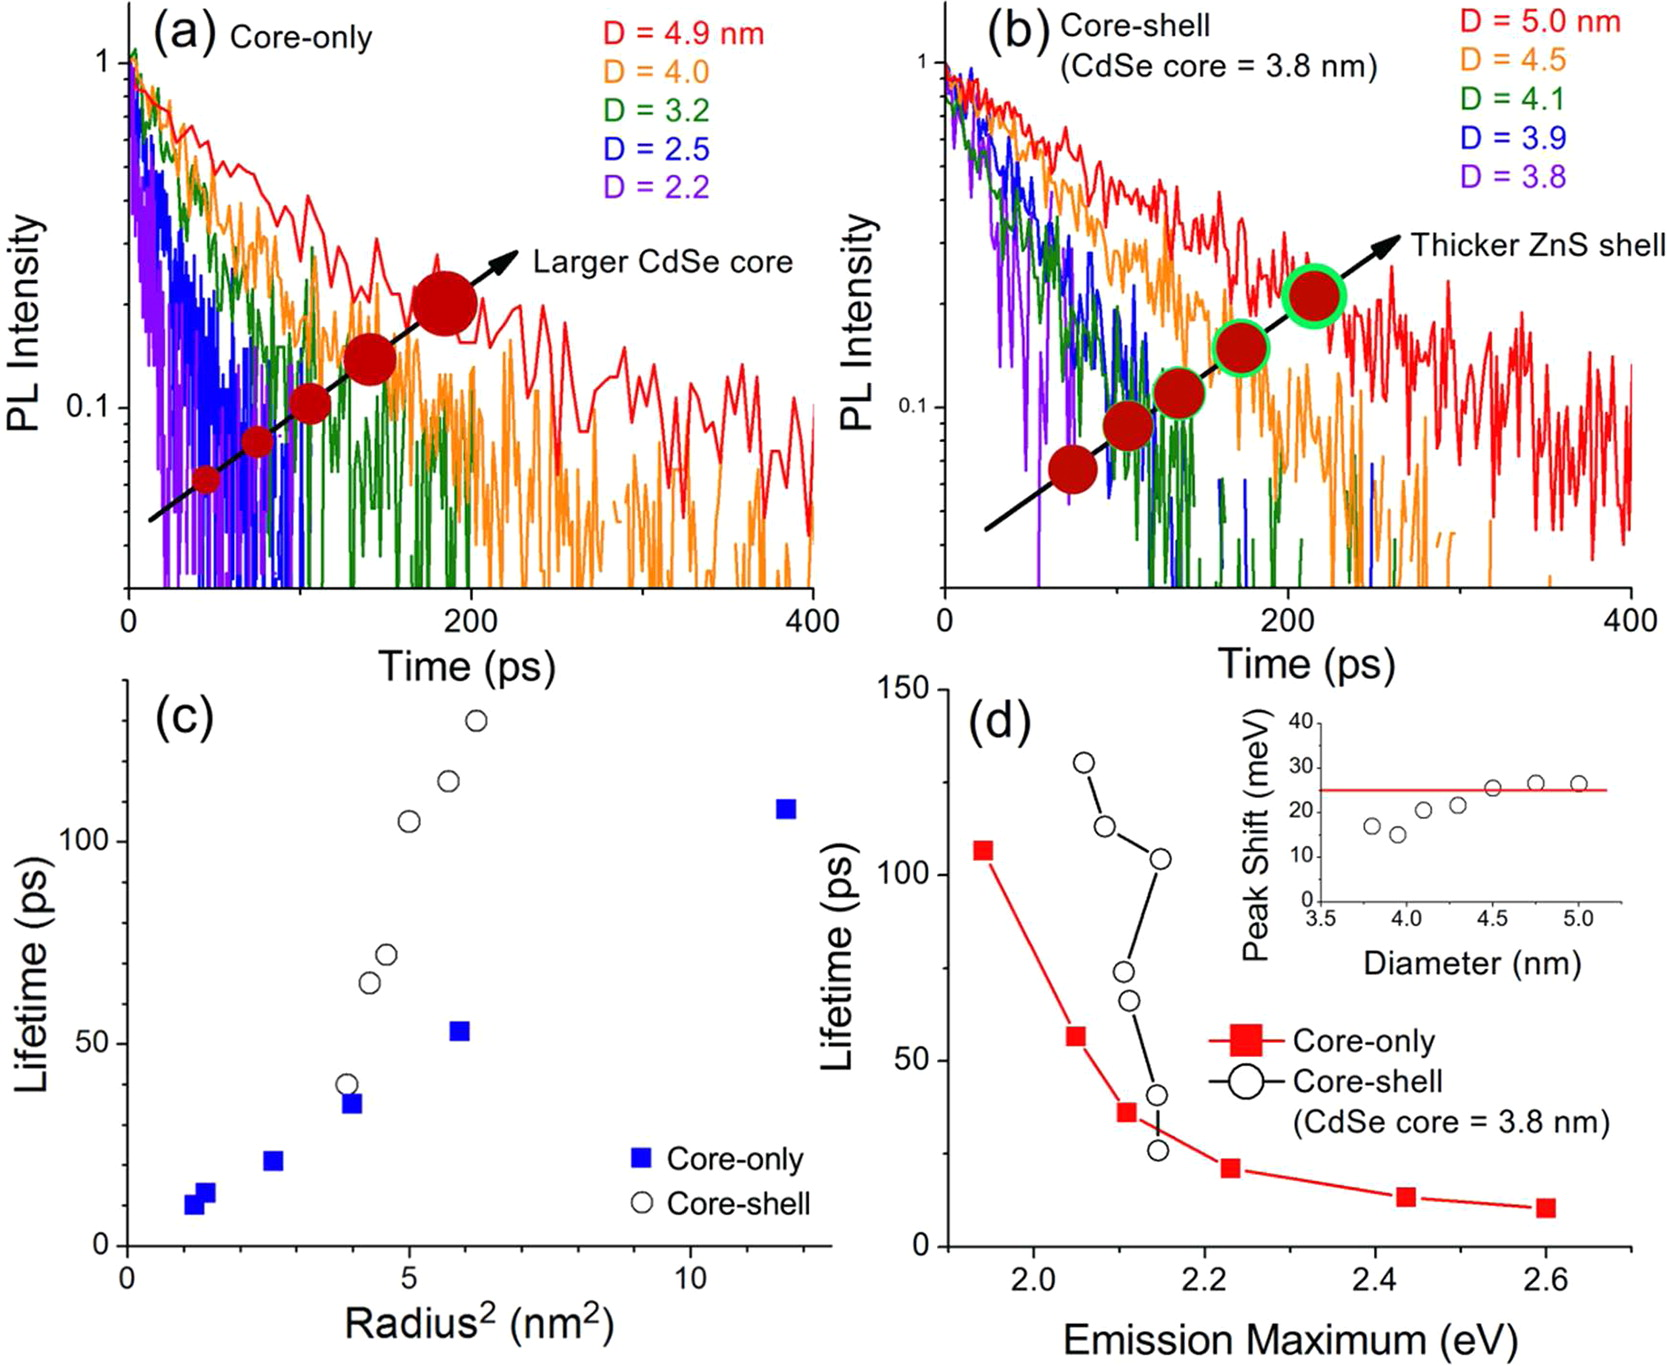
\includegraphics[width=0.75\textwidth]{./Chapter5/plevel3.jpeg}
\caption[PL decay dynamics as a function of particle size and emission energy for core-only and core-shell CdSe NCs.]{(a) Radiative recombination dynamics at 2.6 K produced by spectrally integrating the higher-energy half, or “blue-side”, of the time-integrated PL spectrum for CdSe core-only NCs with indicated diameters. Here, the late-time amplitude has been subtracted from all PL traces to emphasize the subnanosecond decay dynamics. All data have been normalized at early time. (b) Blue-side radiative recombination dynamics for a set of CdSe-ZnS core-shell NCs. For each diameter indicated, the core-shell structure contains a fixed-size 3.8-nm diameter CdSe, while the diameter indicated represents the overall particle size. (c) The blue-side fast-feature decay lifetime measured at 2.6 K for CdSe core-only NCs (blue squares) and CdSe-ZnS core-shell NCs (open black circles) as a function of the radius squared. Note that the x-axis does not convey emission energy because ZnS shells only weakly affect CdSe core emission. (d) Lifetimes of the rapid emission feature as a function measured PL energy at 2.6 K. Emission energy was determined as the maximum of the time-integrated PL data. The red squares indicate CdSe core-only samples, while the open black circles represent CdSe-ZnS core-shell NCs with a 3.8-nm fixed core-size. Inset: Energy shift from early time PL ($t = 0 - 20$ ps) vs late-time PL ($t = 400 - 420$ ps) for the core-shell NCs with indicated fixed-core diameter and varied thickness ZnS shell.}
\label{f:plevel3}
\end{center}
\end{figure}

By modifying the time scale of thermal outflow from the NCs, the growth of an increasingly thick ZnS shell changes the effective thermal conductivity of the composite material constituted by the NCs embedded in an alkane matrix. We estimate the effective thermal conductivity of this system according to Fourier’s law (for spherical particles), yielding the expression $k_{\mathrm{eff}} = \Delta Q/(4\pi R_{NC}\Delta t\Delta T)$.  In this scenario, $\Delta Q$ is the difference in energy between the excitation source and the NC energy gap; it reflects the amount of energy deposited into the NC lattice during intraband carrier cooling and dispersed as heat (Figure \ref{f:plevel1}(a)).  Here, $R_{NC}$, the NC radius, includes the ZnS shell thickness. Acoustic phonon thermal outflow time, as characterized by the lifetime of the rapid emission feature described above, which we point out may be sensitive to the departure time of the last acoustic phonon in the particle, gives $\Delta t$. Finally, $\Delta T$ is given by the difference in temperature between the hot NC lattice and the surrounding matrix. In Figure \ref{f:plevel4}, the effective thermal conductivity ($k_{\mathrm{eff}}$) for a series of matrix-embedded CdSe core-shell NCs decreases with increasing particle size. Increasing the thickness of a ZnS shell thus modifies $k_{\mathrm{eff}}$ of the system from 0.01 W/m/K to 0.002 W/m/K in a controlled manner without modifying the electronic structure of the NCs.  We estimate that for temperatures near 300 K, these $k_{\mathrm{eff}}$ values increase by a factor of $\sim$5 overall, but retain the same functional form.

\begin{figure}
\begin{center}
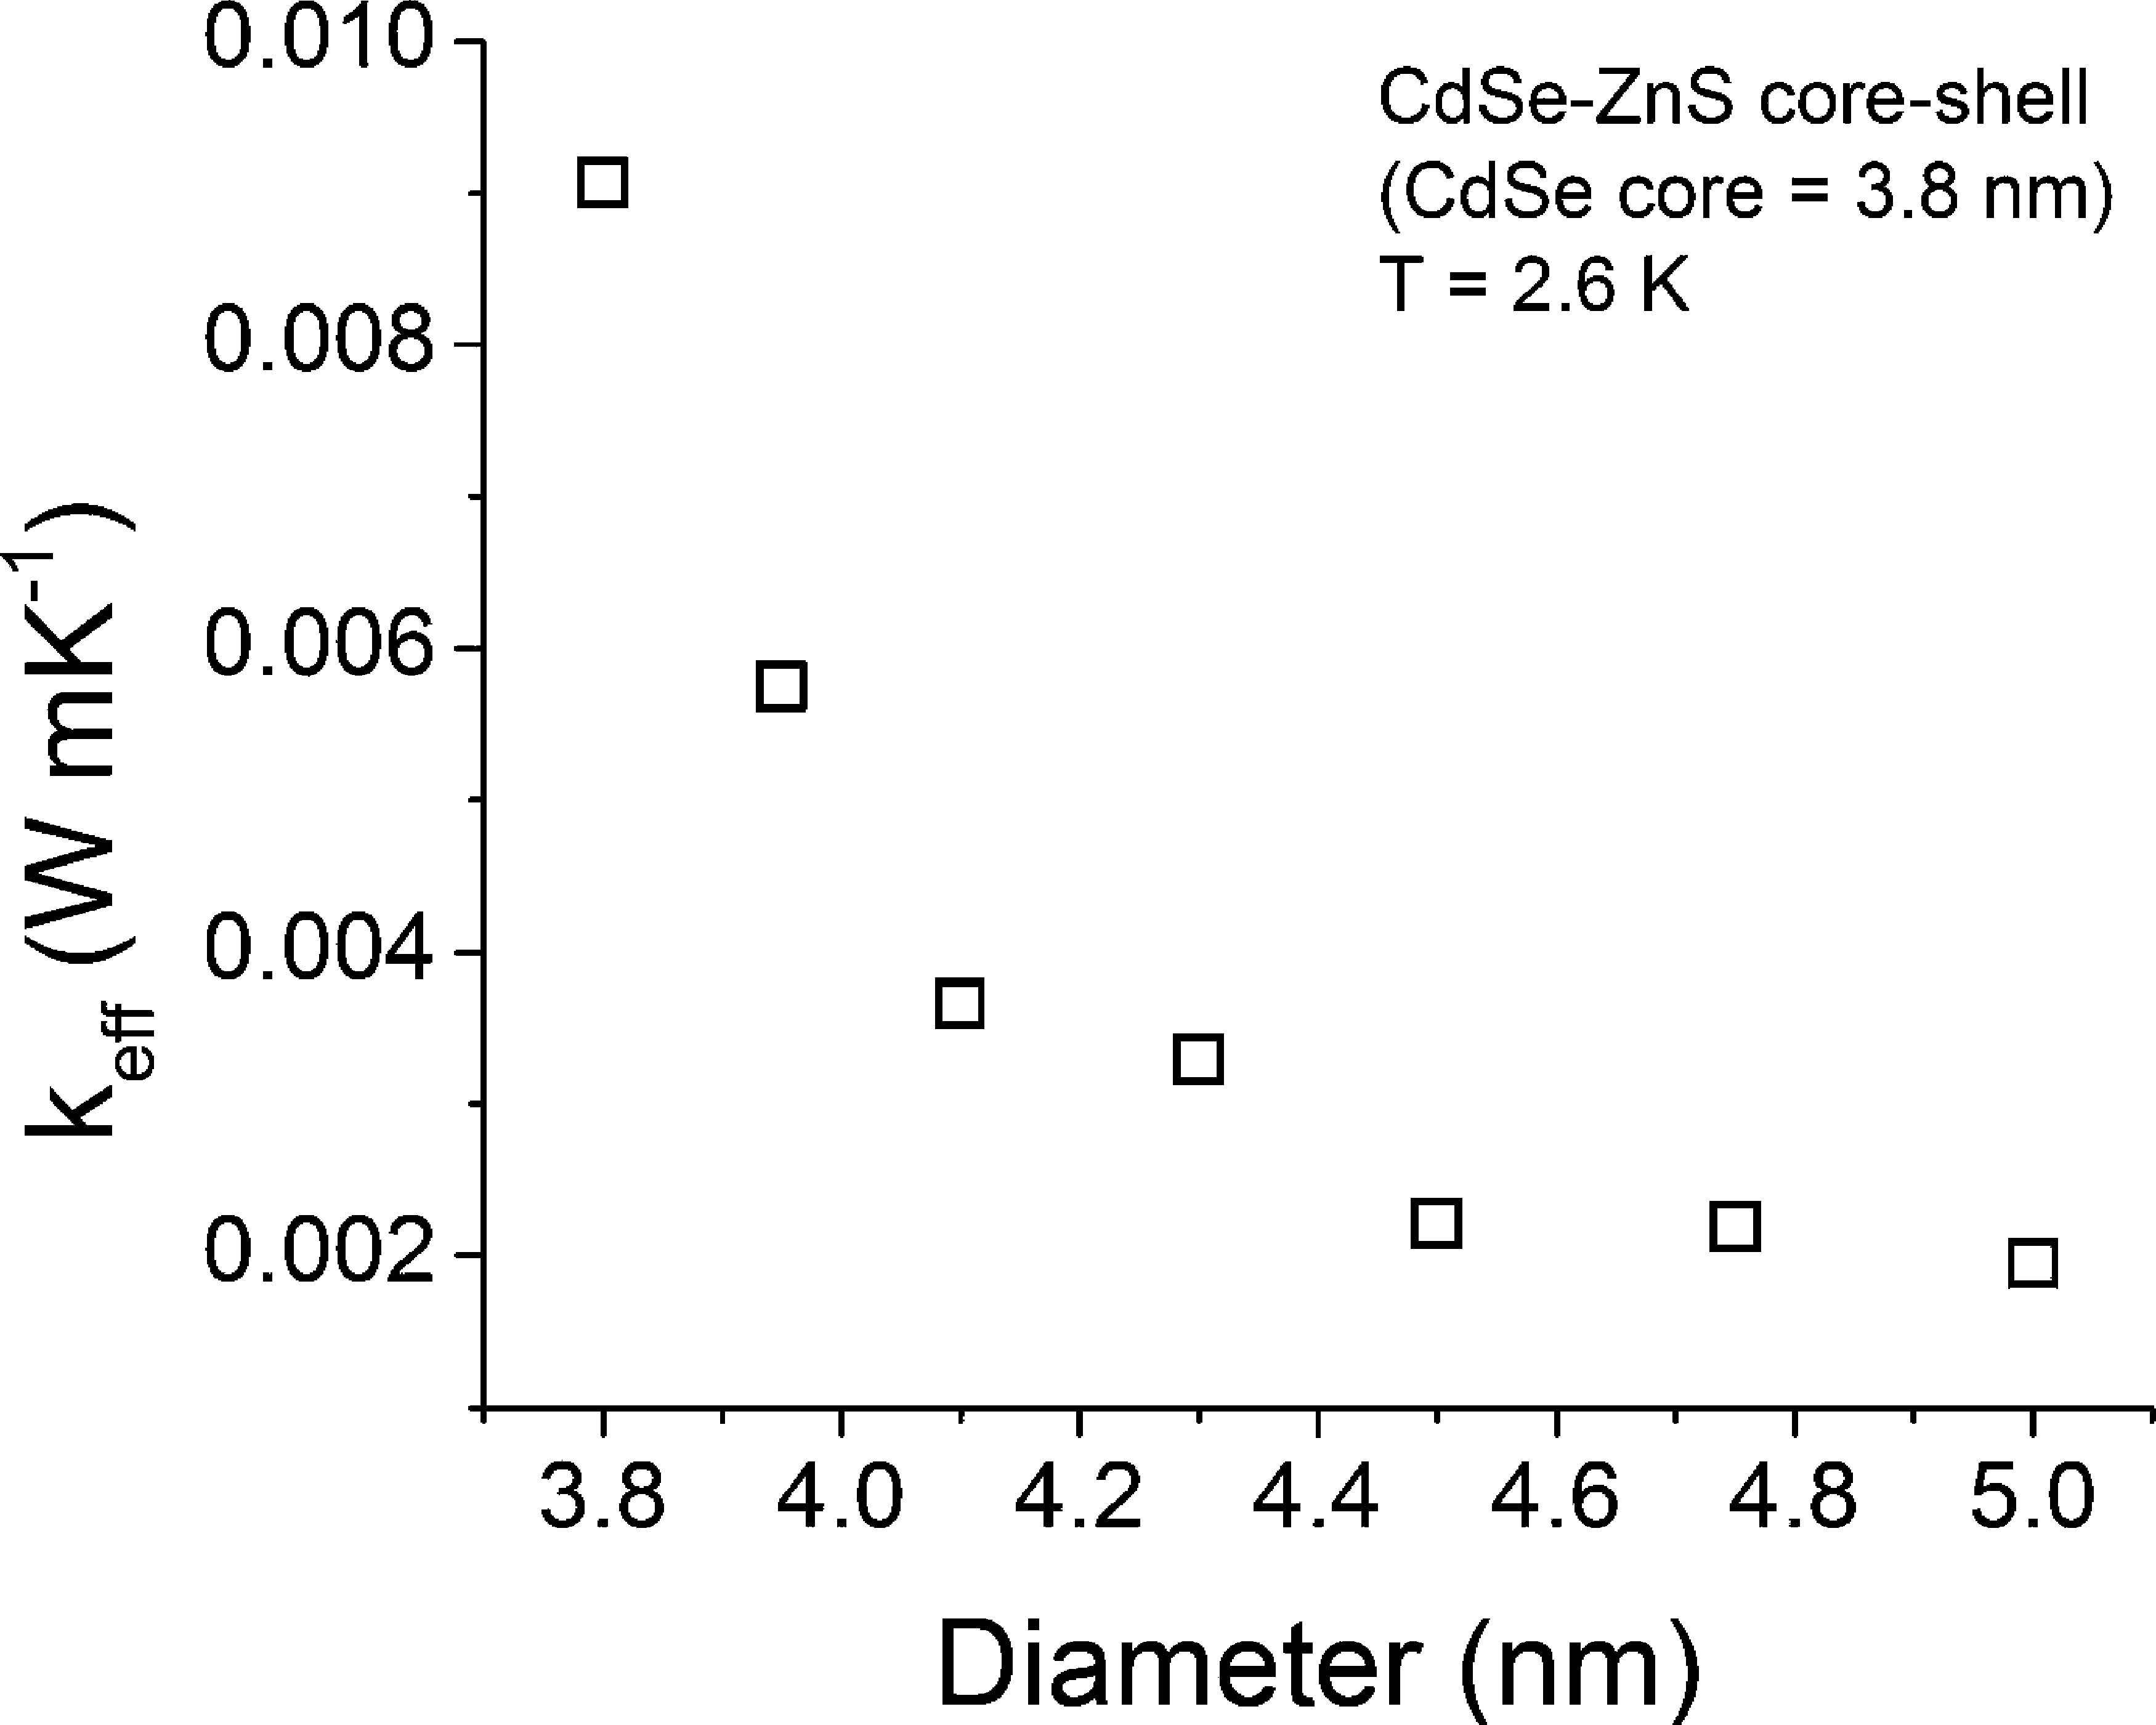
\includegraphics[width=0.75\textwidth]{./Chapter5/plevel4.jpeg}
\caption[Low-temperature effective thermal conductivity as a function of NC diameter for a series of CdSe-ZnS core-shell NCs embedded in an octadecane matrix.]{Effective thermal conductivity as a function of NC diameter for a series of CdSe-ZnS core-shell NCs embedded in an octadecane matrix at 2.6 K. The core-shell NCs, as above, have a fixed-size 3.8 nm diameter CdSe core and variable ZnS shell thickness. The effective thermal conductivity, as described in the text, for the composite comprising the core-shell NCs and the alkane matrix was determined by Fourier analysis and acoustic phonon transport lifetimes.}
\label{f:plevel4}
\end{center}
\end{figure}

\subsection{Conclusions}
In conclusion, we have shown that the growth of an electronically noninteracting ZnS shell permits the extrinsic manipulation of thermal outflow lifetimes for core-shell NCs. We note that the elastic properties of CdSe and ZnS are similar with close acoustic impedance matching at the core-shell interface. Such matching results in a particle that behaves as a larger structure with respect to thermal processes while retaining the electronic properties (such as emission energy) of the CdSe core. In the limit of diffusive transport, this structure changes phonon outflow times as well as the effective thermal conductivity for the NC-matrix system. This particle-level core-shell approach constitutes a bottom-up route to tailor the thermal properties of matrix-embedded NC systems with negligible impact on their optical properties.

\section{Using Surface Ligands to Improve the Thermal Stability of Semiconductor Nanocrystals}

\subsection{Overview}
As discussed in the introductory Chapter of this thesis, nanocrystals are well-known to exhibit depressed melting points relative to their bulk phase, presenting a challenge with regard to the incorporation of these materials into technologies requiring operation at elevated temperatures \cite{goldstein1992melting}. Even at tempereratures below the melting point, thermal processes such as exciton thermal escape or ionization (ejection of either the electron or hole) can lead to a loss of electron-hole pairs and a corresponding quenching of optical activity \cite{valerini2005temperature,yang1997effect, jones2009signatures}. Furthermore, processes such as ligand desorption, surface reconstruction, and sintering can irreversibly alter or degrade desired optoelectronic properties \cite{gao2004nanostructures}. Therefore, strategies to improve the stability and optoelectronic performance of NCs at elevated temperatures are of interest. \par

As demonstrated above, the growth of an optoelectronically non-interacting shell is capable of manipulating the thermal conductivity of CdSe nanocrystals. It was also recently demonstrated to significantly improve thermal stability of CdSe/ZnS core-shell particles relative to core only CdSe particles \cite{rowland2013exciton}. The addition of a wide bandgap semiconductor shell, however, creates an insulating barrier to electrical contact with the core, severely limiting the utility of core-shell particles in applications requiring carrier mobility. In the course of exploring alternative material strategies to improve thermal stability while still permitting electrical and physical access to the core, we explored two structural motifs: recently developed small, inorganic capping ligands and the covalently-terminated surfaces presented by group-IV nanocrystals, such as Si (whereas most binary nanocrystal compositions, including the metal chalcogenides, present surfaces passivated by volatile, ionically bound ligands \cite{porter2008photoconduction}). Experimental work in this area was carried out by Clare Rowland (Schaller group, Northwestern University); below I report my complementary theoretical efforts in exploring each of the areas noted above.

\subsection{Boosting High-Temperature Photoluminescence in InP Nanocrystals}
To briefly summarize the experimental work carried out by Rowland \emph{et al.}, transient absorption and PL spectroscopy demonstrated that passivation of InP NCs with small, inorganic capping ligands (S$^{2-}$ and Sn$_2$S$_6^{4-}$) increased the high-temperature PL intensity from the NCs in a fashion comparable to that of wide-gap semiconductor (ZnS) shell-growth. Figure \ref{f:inp1} summarizes the results of the experiment. \par

\begin{figure}
\begin{center}
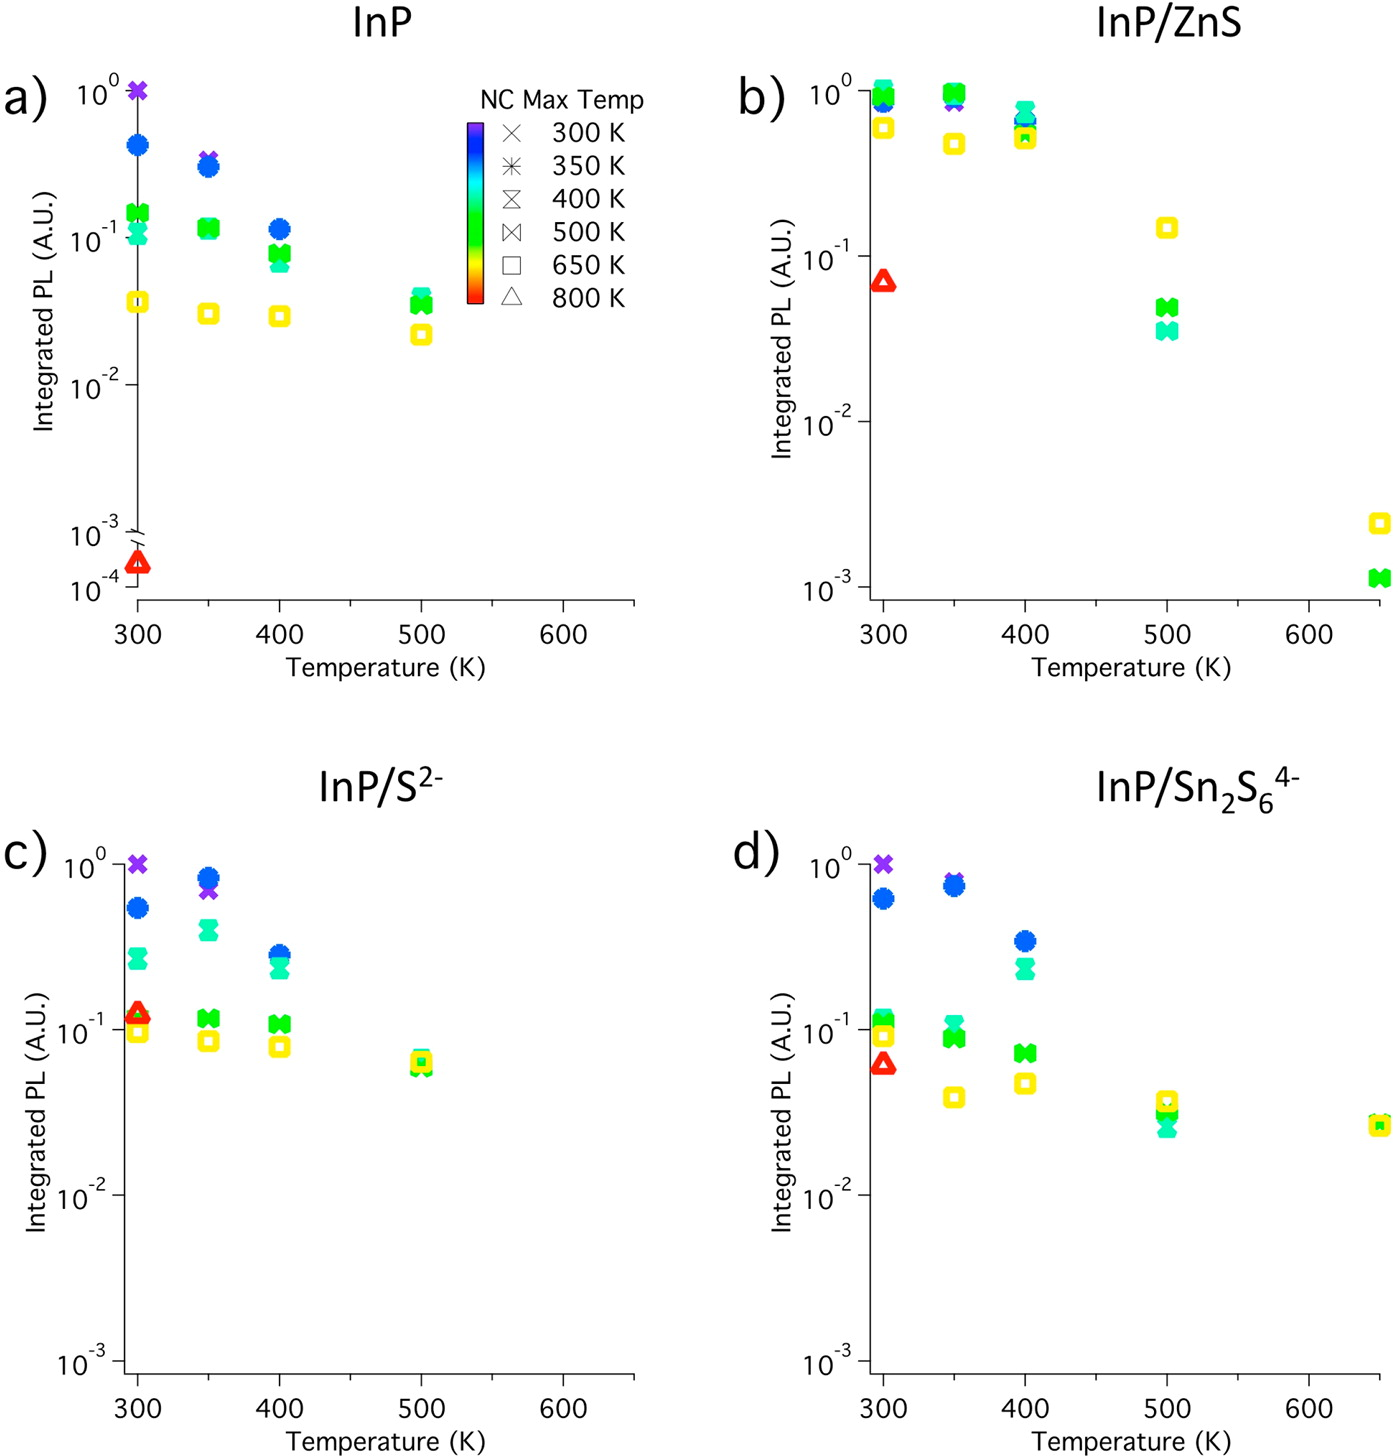
\includegraphics[width=\textwidth]{./Chapter5/inp1.jpeg}
\caption[Integrated PL intensity from InP NCs with four different surface terminations at a variety of temperatures.]{Integrated static PL for InP, InP/ZnS core-shell, InP/S$^{2-}$, and InP/Sn$_2$S$_6^{4-}$ NCs subjected to cyclical heating. Data are plotted as a function of measurement temperature, and symbols and colors correspond to the maximum temperature to which NCs were raised in the previous heating cycle. InP/ZnS and InP/S$^{2-}$ recover more resiliently after heating than do InP and InP/Sn$_2$S$_6^{4-}$ NCs. Data collected and analzyed by Clare Rowland, Northwestern University.}
\label{f:inp1}
\end{center}
\end{figure}

The data presented in Fig. \ref{f:inp1}(a) reveal an order of magnitude loss in PL at 300 K for organically-passivated InP cores following temperature elevation to a mere 400 K, while InP/ZnS cores recover virtually all PL intensity across the same regime. Following heating to higher temperatures (650 K), the organically-passivated InP cores exhibit a loss of 98\% PL intensity as compared to 40\% loss for InP/ZnS core-shell NCs. InP NCs passivated with small, inorganic ligands (S$^{2-}$ and Sn$_2$S$_6^{4-}$) display an intermediate extent of PL recovery following heating, and outperform the organically-passivated InP in this respect by a significant margin. In particular, inorganically-capped samples exhibit appreciable PL even following heating to 800 K, similar to the core-shell sample. \par

These above results are particularly encouraging in light of the fact that the small, inorganic capping ligands examined in this study have been found to enable extremely carrier mobilities in NC films exceeding even those exhibited by organically-passivated samples \cite{talapin2009prospects, lee2011band}. Several factors are important in understanding the improved thermal stability of S$^{2-}$ passivated NCs including the relative thermal stability of the passivating ligand as well as potential differences in electronic structure between organically and inorganically passivated NCs. Theoretical modeling was used to investigate the potential impact of inorganic passivation on NC electronic structure.

\subsubsection{Calculation Details}
Faceted zinc-blende InP nanocrystals with a 1.6 nm-diameter were constructed and passivated with hydrogen and sulfur atoms. Hydrogen passivation was accomplished by placing hydrogen atoms at tetrahedral positions for any In and P atoms having fewer than four bonds. Sulfur passivation was accomplished by placing sulfur atoms in positions corresponding to the lowest energy structure for a S-passivated InP surface. \cite{deng2010surface}. This structure consists of sulfur atoms on the InP surface as well as a layer of sulfur atoms beneath the top layer of In atoms on (001) faces. DFT calculations were carried out using the Vienna Ab-Initio Simulation Package \cite{PhysRevB.54.11169} with the supplied Projector Augemented Wave (PAW) potentials for core electrons \cite{kresse1999ultrasoft}. The NC was placed in the center of an otherwise empty 30 $\times$ 30 $\times$ 30 \r{A} unit cell, which was found to be sufficiently large to prevent spurious interactions between periodic images of the NCs. Electronic structure calculations were carried out at the $\Gamma$ point in the Brillouin zone. Atomic positions for each structure were relaxed until the forces acting on each atom were less than 0.02 eV/\r{A}, after which the electronic density of states (DOS) was calculated for each particle.

\subsubsection{Results and Discussion}

\begin{figure}
\begin{center}
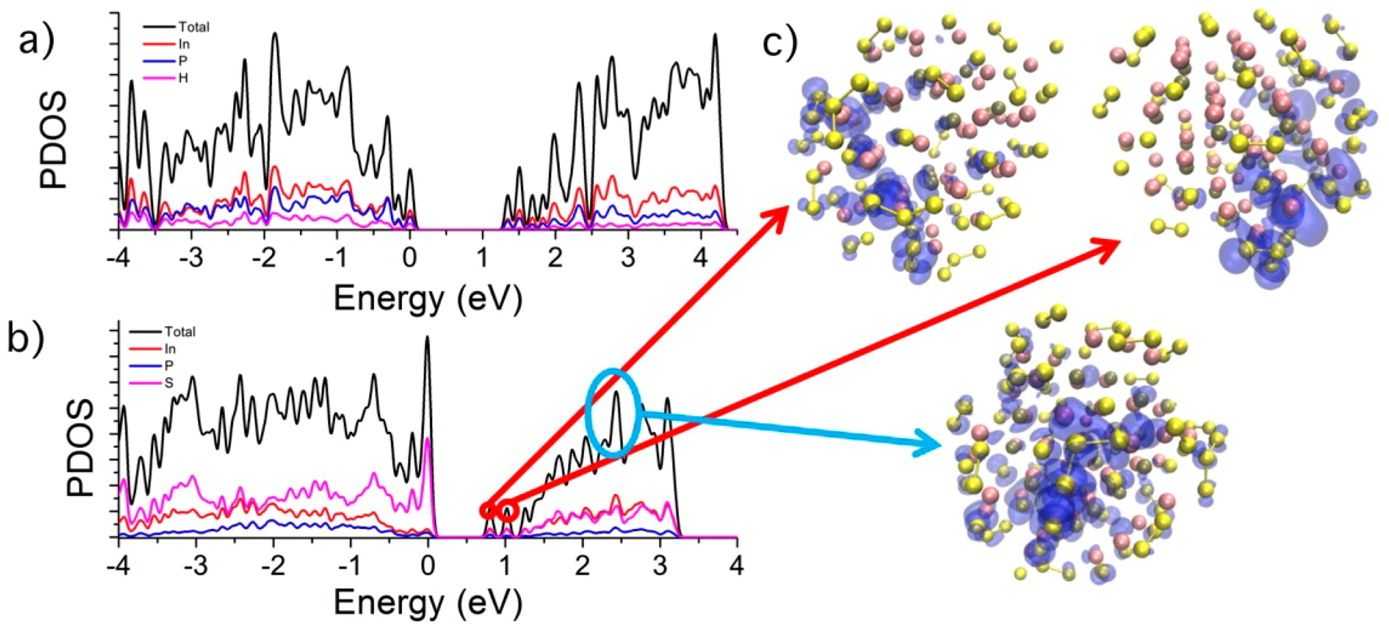
\includegraphics[width=\textwidth]{./Chapter5/inp2.jpeg}
\caption[DFT-dervied electronic structure of H- and S-passivated InP NCs.]{(a) DFT-derived electronic density of states for a hydrogen terminated InP nanocrystal (black curve). The PDOS for each atomic species is also shown: In (red curve), P (blue curve), H(pink curve). (b) DFT-derived electronic density of states for a sulfur terminated InP nanocrystal (black curve). The PDOS for each atomic species is also shown: In (red curve), P (blue curve), S(pink curve). (c) Lowest energy structure for a sulfur-terminated InP nanocrystal with three different charge densities, each associated with a region of the DOS indicated in (b). The red arrows indicate the trap-like states at the conduction band edge, while the blue arrow indicates a "core-like" state with charge density through the nanocrystal structure.}
\label{f:inp2}
\end{center}
\end{figure}

Figure \ref{f:inp2}(a) shows the total and atom-projected DOS for a hydrogen-terminated InP nanocrystal. The total DOS for the sulfur-terminated particle is shown in Figure \ref{f:inp2}(b). In each calculation, the highest occupied molecular orbital (HOMO) has been set to zero energy. Overall, the DOS is qualitatively similar for each structure, with a few exceptions. The valence band maximum for the sulfur terminated particle is dominated by contributions from sulfur atoms, in agreement with previous studies on sulfur-passivated InP (001) surfaces \cite{deng2010surface}. This contribution may be exaggerated compared to the nanocrystals studied experimentally, which are larger and have a correspondingly decreased surface-to-volume ratio. Two small bands are present at the bottom of the conduction band for the S-passivated nanocrystal (Figure \ref{f:inp2}(b)). We find these bands to have trap-like character, rather than being strongly associated with the NC core. Figure \ref{f:inp2}(c) shows the charge density associated with these states projected onto the NC structure. Circles and arrows drawn from Figure \ref{f:inp2}(b) indicate the origin of each charge density plot in Figure \ref{f:inp2}(c). The two small bands that are clearly below the main conduction band localize charge primarily in sulfur p-type orbitals and on In-S species on the NC surface. By contrast, states wholly within the conduction band exhibit charge density more evenly distributed through the NC, as shown in the bottom structure of Figure \ref{f:inp2}(c). Discounting the trap-like states at the conduction band minimum, we find similar energy gaps for the hydrogen-passivated and sulfur-passivated nanocrystal (1.35 and 1.37 eV, respectively). \par

\subsection{Conclusions}
These results suggest that the thermal stability imparted by passivation with inorganic ligands is not due to modification of the NC electronic structure. Instead, negligible differences in the electronic structure point to a temperature-driven change in atomistic conditions, the consideration of which merits a closer investigation of the thermal stability of the surface-passivating media. Degradation of the surface passivants would be expected to lead to surface defects and reconstructions, which would provide precisely the carrier trap sites that could account for irreversible PL loss. As is detailed in the work by Rowland \emph{et al.}, we ultimately attribute the superior high-T optical properties of S$^{2-}$-passivated InP to the extremely low volatility of the passivating ligand, which prevents temperature-induced desorption while still effectively passivating the NC surface. It is significant that S$^{2-}$ ligands do not perturb the NC electronic structure, as these ligands may provide a viable alternative to wide-gap shell growth which provides similar optical and thermal benefits whilst permitting electrical contact with the NC core. 

\subsection{The Impact of Covalent Surface Chemistry on the Thermal Stability of Si Nanocrystals}

\subsubsection{Background}
As demonstrated in this Chapter, the addition of a wide-gap semiconductor shell or small, inorganic passivating ligands such as $S^{2-}$ leads to improved optical performance of NC materials at elevated temperatures. However, most core-only NC compositions are passivated with ionically bound ligands, the volatility of which contributes to temperature-induced loss of desirable optical properties via the formation of trap sites at undercoordinated surface atoms \cite{rowland2013exciton, rowland2013thermal}. A key surface motif remaining unexplored is the covalent bond, the stability of which may yield more thermally robust surface passivation. \par

Silicon NCs are an excellent test bed for this motif given the ability of Si to form covalent bonds with carbon. Furthermore, Si dominates the electronics industry, and the enhanced optical properties of Si NCs relative to bulk Si has led to the suggestion that Si NCs may be useful in a wide variety of technologies. The optical properties of Si NCs are discussed at length the following Chapter. Excitement generated by the superior optical properties of Si NCs has been somewhat tempered by the apparently greatly depressed melting points of these materials, with prior reports noting melting in oxide-terminated Si NCs at as low as one-third of the bulk melting point \cite{goldstein1996melting, hirasawa2006size, lu2009size, wautelet1991estimation}. \par

To assess the role of covalent termination in NC stability, Si NPs terminated with covalently bound dodecane ligands were studied in a fashion similar to the InP NCs discussed in the previous section (see Fig. \ref{f:inp1}). The experimental details and results are reported in the work by Rowland \emph{et al.}\cite{rowland2014silicon}, but are summarized briefly here. \par

\subsubsection{Summary of Experimental Results}
Significant PL intensity was found to persist at temperatures up to 600 K, with PL losses up to 800 K being fully recoverable following a subsequent decrease in sample temperature. These results are surprising in light of previous reported experiments and theoretical work on melting point depression in Si NCs where particles in this size range (2-4 nm-diameter) have been reported to melt at 400 - 500 K \cite{goldstein1996melting, hirasawa2006size, lu2009size, wautelet1991estimation}. To support our experimental results, we analyzed covalently terminated Si NCs using an analytical model of nanocrystal melting as well as atomistic MD simulations. Both theoretical approaches are in agreement with our experimental results and suggest that surface passivation and lattice crystallinity persist well beyond 800 K for the sizes considered here. Overall these results suggest that covalent surface termination may offer optical and thermal benefits akin to shell growth. Our results also point to significantly higher melting points for covalently terminated NCs than those previously reported for oxide passivated particles.

\subsubsection{Phenomenological Model of Size-Dependent Nanocrystal Melting}
Theoretical descriptions of melting at surfaces and interfaces, and by logical extension, nanoparticles, constitute a field unto themselves, and a complete review of this subject is beyond of the scope of this thesis. Here, we focus on a thermodynamic, shape-sensitive model of nanocrystal melting that is well-suited to extremely small ($< \sim$2 nm) NCs \cite{farrell2007binding, wautelet2003phase}. While only some of the NCs experimentally considered fall in this regime, we are most interested in the lowest possible melting point expected for Si NCs considering prior reports of extremely low melting points relative to the bulk phase, and so choose to focus on a model which is known to accurately describe the melting points of the smallest sizes of NCs studied here. The model is derived from an expression of how the isobaric free energy of the (bulk) liquid phase, $G_l(T)$, varies with temperature as compared to the (bulk) crystalline phase, $G_c(T)$, for a fixed composition. Because the melting point, $T_m(\infty)$, is well above the Debye temperature of the solid, the specific heat is approximately constant. Then, the temperature variance of this Gibbs' free energy difference is given by Equation \ref{eq:simelting1}:
\begin{equation}\label{eq:simelting1}
(G_l - G_c)_{\infty} = C - BT
\end{equation}
In Eq. \ref{eq:simelting1}, $C/B = T_m(\infty)$, and $C$ is the latent heat of melting. In general, the $\infty$ subscript denotes the bulk phase. Computing a an analogous relationship for a finite-size cluster of $N$ atoms requires us to consider the effect of surface tensions for the solid and liquid phases:
\begin{equation}\label{eq:simelting2}
N(G_l - G_c) = N(G_l - G_c)_{\infty} + fN^{2/3}(\gamma_l - \gamma_c)
\end{equation}
In Eq. \ref{eq:simelting2}, $f$ is a geometrical factor depending on particle shape, and $\gamma_{l\left(c\right)}$ is the surface tension of the liquid (crystal). By definition, $(G_l - G_c) = 0$ at $T = T_m(r)$ for a particle of radius $r$. Therefore at $T = T_m(r)$, we have:
\begin{align*}
0 = N(G_l + G_c)_{\infty} + fN^{2/3}(\gamma_l - \gamma_c) 
\end{align*}
Plugging Eq. \ref{eq:simelting1} into the above and simplifying:
\begin{align*}
0 &= N(C - BT_m(r))_{\infty} + fN^{2/3}(\gamma_l - \gamma_c) \\
  &= C - BT_m(r) + fN^{-1/3}(\gamma_l - \gamma_c) \\
  &= \frac{C}{B} - T_m(r) + fN^{-1/3}\frac{(\gamma_l - \gamma_c)}{B}
\end{align*}
Recalling that $C/B = T_m(\infty)$, we substitute this into our equation and further simplify:
\begin{align*}
0 &= T_m(\infty) - T_m(r) + fN^{-1/3}\frac{(\gamma_l - \gamma_c)}{B}\\
T_m(r) &= T_m(\infty) + fN^{-1/3}\frac{(\gamma_l - \gamma_c)}{B} \\
T_m(r) &= T_m(\infty)\left[1 + fN^{-1/3}\frac{(\gamma_l - \gamma_c)}{BT_m(\infty)}\right] \\
\end{align*}
Finally, noting again that $BT_m(\infty) = C$, we arrive at Eq. \ref{eq:simelting3}:
\begin{equation}\label{eq:simelting3}
T_m(r) = T_m(\infty)\left[1 + fN^{-1/3}\frac{(\gamma_l - \gamma_c)}{C}\right] 
\end{equation}
The term $fN^{-1/3}$ is directly proportional to the ratio of surface to volume atoms \cite{wautelet2003phase}. Also, note that for a spherical particle, $N = r^3/(r_a^3)$, where $r_a$ is the atomic radius of the element in question. For a spherical particle, the $fN^{-1/3}$ may be recast purely in terms of the atomic radius:
\begin{align*} 
\frac{f}{N^{-1/3}} &= \frac{A}{V} \\
\frac{f}{r/r_a} &= \frac{4\pi r^2}{\left(4/3\right)\pi r^3} \\
\frac{f}{r/r_a} &= \frac{3}{r} \implies f = \frac{3}{r_a}
\end{align*}
Plugging this, along with the relationship between $N$ and $r_a$ described above, into Equation \ref{eq:simelting3} yields:
\begin{equation}\label{eq:simelting4}
T_m(r) = T_m(\infty) \left(1 - \frac{c'}{n}\right)
\end{equation}
In the above equation, $n = N^{1/3}$ and $c'$ is a collection of material-dependent constants: $c' = 3\left(\gamma_c - \gamma_l\right)/r_aC$. While addressing the specific case of small, group-IV semiconductor nanoparticles, Farrell and co-workers examined \emph{ab-initio} calculations of binding energy in these materials and $c'$ is roughly unity for small ($\sim$2 nm) particles and that the the linear dependence of $T_m(r)$ on $n$ is better described by a $1/n^2$ dependence than a $1/n$ dependence \cite{farrell2007binding}. Implementing these empirical corrections we arrive at the final expression for the dependence of nanoparticle melting point on cluster size:
\begin{equation}\label{eq:simelting5}
T_m(n) = T_m(\infty)\left[1 - \left(\frac{1}{n}\right)^2\right]
\end{equation}
While this model does predict NC $T_m$ size dependence, it does not account for atomistic details such as covalent surface chemistry, which may significantly impact thermal stability and $T_m$.

\subsubsection{Molecular Dynamics Simulations of Nanoparticle Melting}
We use MD simulations to gain atomistic insight into the temperature-dependent behavior of Si NCs. Faceted Si NCs were created using the Wulff construction and experimentally known surface energies \cite{hong1998effect}. For simplicity and computational tractability, Si NC surfaces were passivated with hydrogen atoms. Interactions between atoms were modeled using an empirical second-order reactive bond-order potential \cite{schall2008elastic}. The potential used here has been shown to reproduce well the elastic properties of crystalline Si and the energetics of the H-passivated Si surfaces \cite{murty1995empirical}. Si NCs were first relaxed until the forces between atoms were less than 0.02 eV/\r{A}. Following relaxation, NCs were subjected to a temperature annealing procedure. Atomic velocities were rescaled to a particular temperature in steps of 100 K. After each rescaling, NCs were allowed to equilibrate for 5 ps in the NVT ensemble. Following equilibration, NCs were simulated for another 2 ps to yield production-run data. All MD calculations were carried out using the General Utility Lattice Program \cite{gale2003general}. \par

\begin{figure}
\begin{center}
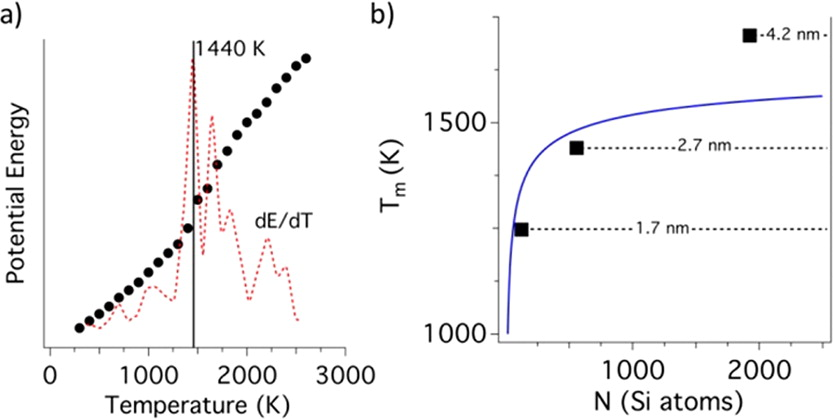
\includegraphics[width=\textwidth]{./Chapter5/simelting1.jpeg}
\caption[MD simulations of Si NC melting for multiple NC sizes.]{(a) Average potential energy vs temperature for a 2.6 nm-diameter, H-passivated Si NC. The data points represent an average of 2 ps of simulation of an equilibrated NC at the given temperature. The dashed line indicates the first derivative of the potential energy vs temperature. (b) Melting point as a function of Si NC temperature via multiple methods. The solid blue line indicates the prediction of the modified phenomenological model (Eq. \ref{eq:simelting5}), while the square data points indicate first derivative maxima indicating melting temperatures from MD simulations.}
\label{f:simelting1}
\end{center}
\end{figure}

Figure \ref{f:simelting1} displays the potential energy of a 2.6 nm Si NC (558 atoms) at each temperature step, averaged over the 2 ps production run. A discontinuity, emphasized in the first derivative, is evident at 1440 K and indicates a solid-liquid transition ($T_m$) that is depressed relative to $T_{m, bulk} = 1687$ K \cite{goldstein1992melting}. By similarly treating both a smaller and larger Si NC, a positive correlation appears between size and $T_m$, consistent with thermodynamic considerations. The MD simulations qualitatively agree with the phenomenonological model and prior MD studies utilizing the Stillinger-Weber potential \cite{fang2005investigation}. Agreement with the model is markedly poorer for the 4.2 nm particle, although this is perhaps not surprising in light of the fact that the model here was developed with extremely small particles in mind. Furthermore, the melting point of the largest particle seems to approach $T_{m, bulk}$; this is perhaps because the interaction potential utilized herein is known overestimate $T_{m, bulk}$ \cite{erhart2005analytical}. Regardless, both methods predict that $T_m$ values exceed the temperatures examined experimentally even for the smallest size of NC considered. \par
\subsection{Conclusions}
While the potential utilized in these MD simulations is parameterized to capture bond breaking and formation \cite{schall2008elastic}, the simulations do not exhibit ligand desorption until temperatures in excess of 1600 K. While further investigation is certainly warranted to model this process with a higher degree of accuracy, our theoretical effots support the conclusions suggested by the PL data presented in the work by Rowland \emph{et al.} \cite{rowland2014silicon}: Covalently-passivated Si NCs exhibit enhanced thermal stability relative to ionically-capped nanocrystals such as CdSe and InP.
\chapter{Photoluminescence in Silicon Nanoparticles}

Work in this Chapter is adapted from the following papers:
\begin{itemize}
\item Hannah, D.C.; Yang, J.; Podsiadlo, P.; Chan, M.K.Y.; Demortiere, A.; Gosztola, D.J.; Prakapenka, V.B.; Schatz, G.C.; Kortshagen, U.R.; Schaller, R.D. \emph{Nano Letters} \textbf{2012}, 12, 4200
\item Hannah, D.C.; Yang, J.; Kramer, N.J.; Schatz, G.C.; Kortshagen, U.R.; Schaller, R.D. \emph{ACS Photonics} \textbf{2014}, 1, 960
\end{itemize}
\section{Overview}

Although bulk crystalline silicon dominates consumer electronics, the indirect character of its lowest-energy interband transition frustrates utility in optoelectronic devices. Specifically, optical emission and band-edge absorption in this material occurs \emph{via} phonon-assisted transitions between $\Gamma_{\mathrm{valence}}$  and X$_{\mathrm{conduction}}$ symmetries in Brillouin space \cite{hull1999properties}. Because these second-order momentum-conserving processes take place inefficiently, bulk silicon absorbs and emits photons weakly. On the other hand, nanosized silicon structures such as porous silicon \cite{canham1990silicon}, silicon quantum dots formed by self-assembly in SiO2 matrices \cite{shimizu1998optical,zacharias2002size}, and organically terminated colloidally prepared nanocrystals (NPs - as we study both amorphous and crystalline particles later in this Chapter, we utilize the abberviation "NP" rather than "NC" for the duration of this Chapter) \cite{mangolini2007plasma,erogbogbo2010vivo,mangolini2005high,pettigrew2003solution,hessel2011synthesis,holmes2001highly,atkins2011femtosecond} exhibit significantly enhanced emission efficiencies with PL (PL) quantum yields that can exceed 50\% \cite{PhysRevB.80.115407,jurbergs2006silicon,Wilson19111993}.  While the high PL efficiencies invite applications in nontoxic biolabeling \cite{erogbogbo2010vivo} and energy-efficient light-emitting diodes \cite{ng2001efficient,cheng2011high} the mechanisms and origin of bright PL in nanosized silicon have remained a subject of discussion for more than two decades \cite{canham1990silicon, PhysRevB.49.16845,PhysRevLett.88.097401,reboredo2005theory,
de2010red,PhysRevB.61.4485,cullis1991visible,PhysRevLett.100.067401,saar2009PL,kovalev1999optical,PhysRevLett.72.1514,PhysRevLett.81.2803, godefroo2008classification}. \par

Silicon nanocrystals generally exhibit both a high-energy and low-energy photolumiscence band. Reports vary considerably in the origins attributed to each band and even more so in the timescales reported for the lifetime of each band, which span the picosecond to microsecond timescales. Relevant previous work related to each PL band will be discussed below. In this Chapter, we report the pressure-dependent PL from plasma grown, alkane-terminated colloidal particles. We find a systematic PL red shift that matches the X$_{\mathrm{conduction}}$-to-$\Gamma_{\mathrm{valence}}$ transition of bulk crystalline silicon. These results, reinforced by calculations, suggest that efficient PL, frequently attributed to defects, arises instead from core-states that remain highly indirect despite quantum confinement. \par

We also examine ultrafast, high-energy PL produced from such Si nanocrystals as a function of both particle size and lattice crystallinity. In particular, we quantify the decay time and spectral profiles of nominally few-picosecond direct-gap emission previously attributed to phononless electron-hole recombination. We find that the high-energy (400-600 nm, 2-3 eV) PL component consists of two decay processes with distinct time scales. The fastest PL exhibits an $\sim$30 ps decay constant largely independent of emission energy and particle size. Importantly, nearly identical temporal components and blue spectral features appear for amorphous particles. We thus associate high-energy, rapid emission with an amorphous component in all measured samples, as supported by Raman analysis and MD simulation. Based on these observations, we advise that the observed dynamics proceed too slowly to originate from intraband carrier thermalization and instead suggest a nonradiative origin associated with the amorphous component.

\section{The Origin of Long-Lived, Low-Energy Photoluminescence in Si Nanoparticles}

High surface-to-volume ratios, broad particle size distributions, extrinsic effects of encapsulation matrices and material defects, together with complex PL recombination dynamics, all contribute to a lack of consensus regarding the origin of PL in nanosized silicon. Overall, two origins largely govern the discussion \cite{saar2009PL}.  First, a quantum confinement model, well-known to accurately describe properties of several direct-gap nanomaterial compositions, invokes disruption of the stringent relationships between carrier energy and translational momentum as electronic density of states (DOS) becomes discrete for particle sizes comparable to or smaller than the exciton Bohr radius ($\sim$4.2 nm). Such confinement effects can greatly enhance electron-hole recombination and may impart direct gap character to the lowest-energy electronic transitions \cite{PhysRevLett.72.1514}, which would bolster optoelectronic applications. The quantum-confinement model draws support from observations of characteristic-phonon-assisted PL \cite{PhysRevLett.81.2803}, fast (nanosecond) decay times \cite{PhysRevLett.100.067401,english2002size,kusova2010brightly,groenewegen2010excited}, correlations of particle size with emission energy \cite{Wilson19111993,kovalev1999optical,english2002size,mastronardi2011preparation}, and sensitivity of PL spectra to large magnetic fields \cite{godefroo2008classification}.  The second model instead attributes the high-efficiency PL to surface states wherein any quantum-confined core states that may exist do not produce substantial emission. Instead, excited carriers rapidly relax into lower-lying defect states that slowly radiate \cite{PhysRevB.49.16845,PhysRevLett.88.097401,godefroo2008classification,PhysRevLett.100.067401,PhysRevLett.76.2961,PhysRevB.48.11024,PhysRevB.84.085321}. In this model, chemical details of the crystal surface termination, such as varied abundance and distributions of surface moieties, as well as surface reconstructions, yield tuning of the emission energy largely independently of any particle core-states. Experimental support for the surface-state model arises from observables such as broad emission spectra, sensitivity to chemical treatments \cite{PhysRevLett.82.197}, insensitivity of PL spectra to large magnetic fields \cite{godefroo2008classification}, and long-lived PL decay features (microseconds time scale) \cite{PhysRevLett.100.067401,PhysRevLett.82.197,vzidek2010femtosecond}, which seem inconsistent with the discrete translational-momentum-relaxed DOS of quantum-confined core states. \par

In this thesis, we examine both X-ray diffraction (XRD) and PL as functions of pressure imparted using a diamond anvil cell for multiple samples of highly crystalline, plasma-synthesized, alkane-terminated colloidal Si NPs with the goal of obtaining insights regarding the origin of the efficient PL. From XRD, we first determine the diamond-phase bulk modulus of multiple Si NP sizes and find that obtained moduli closely match the bulk constant in distinction from NPs formed from binary semiconductors \cite{jiang2004phase}. We also observe several crystal phases including Si(I), Si(V), Si(VII), and amorphous Si (a-Si). The structural studies are reported in the following Chapter. In this Chapter, we focus on optical characterization. In pressure-dependent PL studies, we find that in all cases the emission energy closely follows the pressure-dependence of the bulk-phase, band-edge deformation potential associated with the X-to-$\Gamma$ transition. Taken together, this data clearly indicates that the long-lived but efficient PL arises from core-states with indirect-gap character rather than from surface states in these samples. Lastly, we show from calculations that the energy shift is consistent with delocalized NP-core band-edge states using a combination of MD for pressurization and DFT for electronic properties, regardless of the presence or absence of a common oxide surface defect.  

\subsection{Plasma Synthesis of Si Nanoparticles}

The Si NPs studied here were fabricated by room-temperature plasma dissociation of SiH$_4$ using a system described previously \cite{mangolini2007plasma}. A mixture of SiH$_4$/He (5\%/95\% by volume) and argon was introduced into a quartz 13.56 MHz radio frequency (30-100 W) plasma reactor with 6.3 mm inner diameter and 9.5 mm outer diameter, at flow rates of 13 and 35-100 standard cubic centimeters per minute (sccm), respectively. Variation of the plasma power permits tunability of the Si NP crystallinity from highly amorphous to highly crystalline.  Highly crystalline samples were utilized in all pressure-dependent experiments.  The properties of less crystalline and amorphous particles will be explored in later sections of this thesis. An additional H$_2$ flow (100 sccm) was injected at the end of the plasma region to initially H-terminate the NP surfaces. NP size was controlled by particle collection pressure and examined by XRD. Indicated NP radii result from Scherer analysis of diffraction peaks. The Si NPs were collected on mesh filters and then ultrasonicated to obtain a suspension in a mixture of 1-dodecene ligand and mesitylene solvent with a ratio of 1:5 by volume with a specific volume of 3.3 mL of mesitylene per milligram of NPs. The suspension was transferred into a flask reactor and refluxed under N$_2$ flow at 215 $^{\circ}$C. Surface functionalization with dodecane was indicated by transformation of an initially cloudy suspension into a clear solution. The NPs were dried under vacuum at 150 $^{\circ}$C and redissolved in hexane. All steps were carried out in an inert nitrogen-gas environment. PL quantum yields were measured using a silicon CCD, a 400 nm light-emitting diode excitation source, and integrating sphere.

\subsection{Pressure-Dependent Photoluminescence in Si Nanoparticles}

\subsubsection{Experimental Details}
Si NPs were dissolved in ethylcyclohexane and loaded into a diamond anvil cell under a nitrogen atmosphere. A small ruby crystal was placed in the pressure cell along with the NP solution for independent determination of applied pressure \emph{via} ruby R1 fluorescence. PL spectra were produced by exciting at 473 nm with a continuous-wave laser through a long-working distance 10$\times$ objective. The same objective collected PL and directed PL photons to a 300 mm spectrograph outfitted with liquid nitrogen-cooled silicon and InGaAs array detectors. Time-correlated single photon counting (TCSPC) was produced using a 2 kHz, 405-nm laser diode, grating spectrograph, and avalanche photodiode.
\subsubsection{Basic Characterization of Plasma-Synthesized Si Nanoparticles}
Figure \ref{f:sipressure1}(a) shows static PL spectra collected for different NP samples at ambient pressure. XRD-derived NP sizes decrease with increasing PL energies as generally expected for a quantum-confined semiconductor. For the bluest-emitting NP sample, we note that the PL energy is $\sim$38\% higher than the bulk-phase energy gap. All measured samples exhibited quantum yields in the tens of percent range. TCSPC for the samples showed that the efficient PL signals arise due to slow radiative processes, characterized in Figure \ref{f:sipressure1}(b) as exhibiting a fairly single exponential decay with a 75.8 ($\pm$0.3) $\mu$s lifetime. Furthermore, transmission electron microscopy, selected area electron diffraction, and XRD each indicated highly crystalline particles (Figure \ref{f:sipressure1}(c)). Transmission electron microscopy confirmed the average particle sizes determined by XRD and established a particle size dispersion of $\sim$20\% for each of the samples examined herein. \par

\begin{figure}
\begin{center}
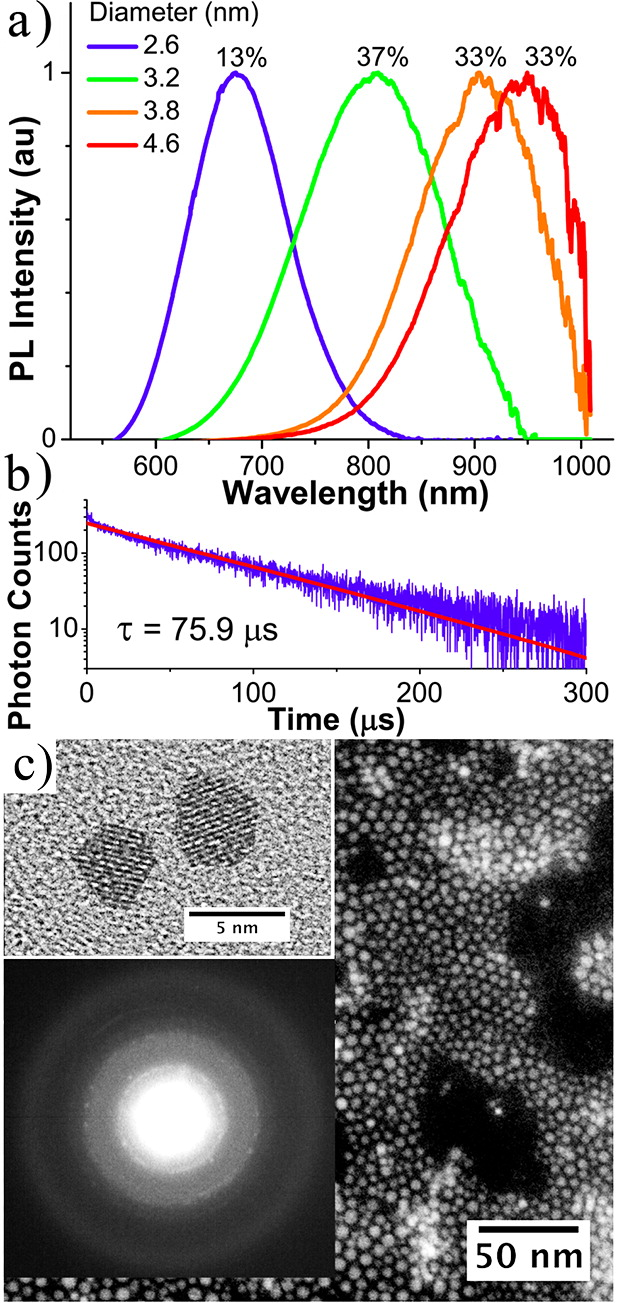
\includegraphics[width=0.35\textwidth]{./Chapter6/sipressure1.jpeg}
\caption[Basic characterization of various sizes of plasma-synthesized Si NPs.]{(a) Ambient pressure PL spectra of silicon NPs with indicated average NP diameters and PL quantum yield. Loss of detector sensitivity beyond 1020 nm artificially influences the largest NP sample spectrum. (b) Time-correlated single photon counting of a 2.6 nm diameter NP sample at ambient pressure measured at 680 nm shows a highly single-exponential decay with a 75.8 $\mu$s lifetime. (c) Transmission electron micrographs of the 3.2 nm sample (main panel). The high-resolution TEM image in the upper inset shows high crystallinity that is also apparent in selected area electron diffraction (lower inset).}
\label{f:sipressure1}
\end{center}
\end{figure}

\subsubsection{Optical Properties of Si Nanoparticles Under Pressure} 
Substantial structural characterization of Si NPs at elevated was performed, the details of which are reported in the following Chapter.  Here, we focus on characterization of the optical properties of the NPs as a function of applied pressure.  Figure \ref{f:sipressure4}(a) displays spectrally resolved PL of the 2.6 nm diameter Si NPs for a range of hydrostatic pressures.  For each pressure, the PL spectrum appears Gaussian with a clearly identifiable emission maximum. Here, increasing pressure produces a distinct red shift of the PL as well as a reduced integrated intensity. Figure \ref{f:amsi4}(b) plots the PL centroid calculated from the data in Figure \ref{f:amsi4}(a) as well as similar measurements performed for the other three Si NP samples. In addition, we plot trend lines for the bulk phase derived from literature sources \cite{PhysRev.98.1755, slykhouse1958effect}.  Linear fitting of the PL emission maximum versus pressure for the different samples yields values of -17.2, -14.2, -21.1, and -21.3 meV/GPa for mean particle diameters of 2.6, 3.2, 3.8, and 4.6 nm, respectively. These band gap dependences on pressure were independent of pressure change direction showing no hysteresis provided that we did not exceed the phase transition near $\sim$20.5 GPa. The observed PL energy dependences on pressure closely agree between samples and also agree with the reported values of −15 and −20 meV/GPa for the band gap of bulk silicon \cite{PhysRev.98.1755, slykhouse1958effect, welber1975dependence}. 

\begin{figure}
\begin{center}
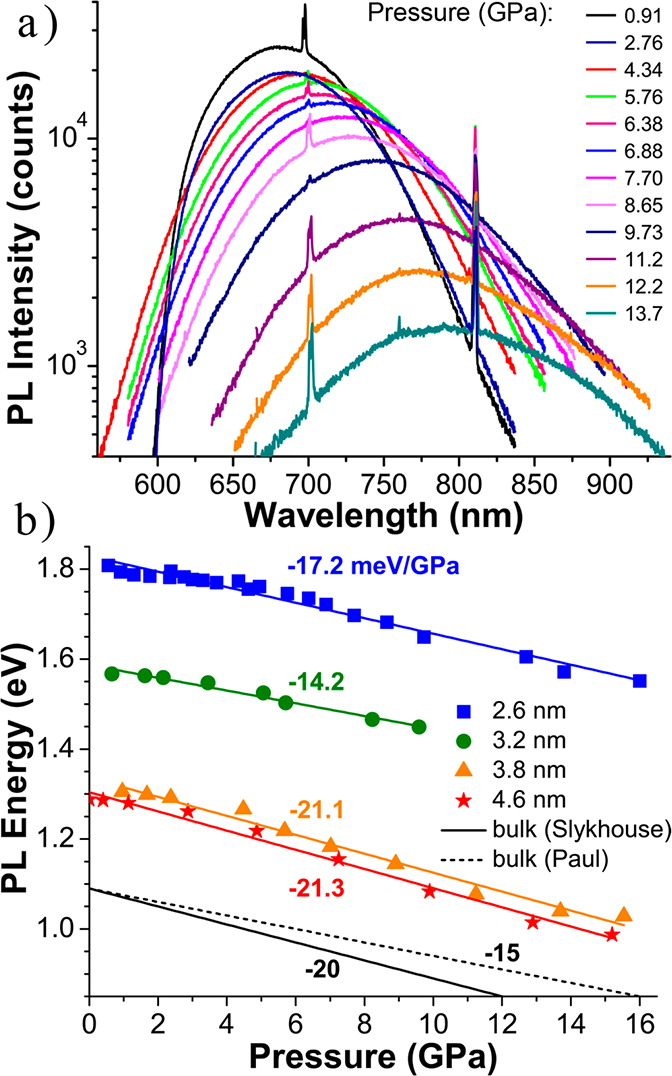
\includegraphics[width=0.5\textwidth]{./Chapter6/sipressure4.jpeg}
\caption[Pressure-dependent PL spectra of plasma-synthesized Si NPs.]{PL spectra of 2.6 nm diameter Si NPs exhibit a red shift as a function of applied pressure. Ruby R1 fluorescence gives rise to the narrow spectral feature near 700 nm and second-order diffraction of the excitation laser produces the narrow feature near 810 nm.  (b) The PL centroid emission energy as a function of pressure for all samples exhibits a shift to lower energy with pressure and closely follows the dependence exhibited by bulk silicon taken from two different sources \cite{PhysRev.98.1755, slykhouse1958effect}.}
\label{f:sipressure4}
\end{center}
\end{figure}

In crystalline semiconductors, compression of the bulk-phase crystal lattice induces energetic changes in band positions. In bulk silicon, the band-edge X$_{\mathrm{conduction}}$-to-$\Gamma_{\mathrm{valence}}$ transition red shifts with increasing pressure while the higher-energy $\Gamma$-to-$\Gamma$ direct-gap blue shifts. The lowest-energy “band-edge” transition arises from two terms in quantum-confined systems corresponding to the bulk energy gap, $E_{bulk}$, plus a quantum-confinement energy term, $E_{QC}$, related to the particle size in comparison to the exciton Bohr radius. In the pressure range examined for the optical studies, NP-volume reduction upon compression imparts negligible changes in radius (at 15 GPa the particle is still $\sim$89\% of its ambient pressure volume, so $<$4\% change in radius) and thus negligible changes in quantum confinement energy. However, the bulk deformation potential produces large changes in the lowest-energy transition \emph{via} the $E_{bulk}$ contribution as reflected in the bulk-phase pressure dependence (Figure \ref{f:sipressure4}(b)). By contrast, surface states are expected to form highly localized excitations that would yield less sensitive dependence of PL energy on pressure. The concurrence of both the sign and amplitude of the pressure-dependent PL shift together with the size-independent bulk modulus of silicon suggests a core-derived origin for the emitting state in these Si NPs. In the range of NP sizes studied, our measurements provide evidence that the efficient PL from Si NPs arises from the X$_{\mathrm{conduction}}$-to-$\Gamma_{\mathrm{valence}}$ indirect transition despite substantial quantum confinement, consistent with the interpretation provided by Brus \cite{Wilson19111993}.  \par

To substantiate the claim that the observed pressure dependence of the PL peak originates from bulk-like Si states rather than surface moieties, we present pressure-dependent DFT calculations of energy gap for a model Si NP.  Specifically, we used the Vienna Ab Initio Simulation Package (VASP) \cite{PhysRevB.54.11169} with supplied Projector Augmented Wave potentials \cite{kresse1999ultrasoft} for core electrons.  A 2 nm diameter, hydrogen-passivated, faceted Si nanocrystal was constructed from known surface energies of H-passivated Si (100), (110), and (111) surfaces \cite{hong2000equilibrium} using the Wulff construction. For each pressure, the model H-terminated Si NP \cite{PhysRevB.37.6991} is compressed by hydrostatic pressure using an inert fluid comprising 108 000 particles with classical MD (MD) methods \cite{martovnak2002pressure}, and the energy gap between the highest occupied and lowest unoccupied molecular orbitals (HOMO and LUMO, respectively) was then calculated using DFT for 11 images within the MD trajectory. Further details regarding these calculations can be found in Appendix D. The effect of a common surface defect, a Si-O-Si, was also investigated and the results are shown in Figure \ref{f:sipressure5}(a,b). We find that the HOMO-LUMO gap of the Si NP decreases linearly with increasing pressure, as observed in the experiment, regardless of the presence or absence of the surface defect group. Charge density iso-surfaces for the HOMO and LUMO at pressures of 1 and 20 GPa are shown in Figure \ref{f:sipressure5}(c,d). We see that the HOMO and LUMO are extended and not localized on the surface, regardless of existence of the surface defect. \par

\begin{figure}
\begin{center}
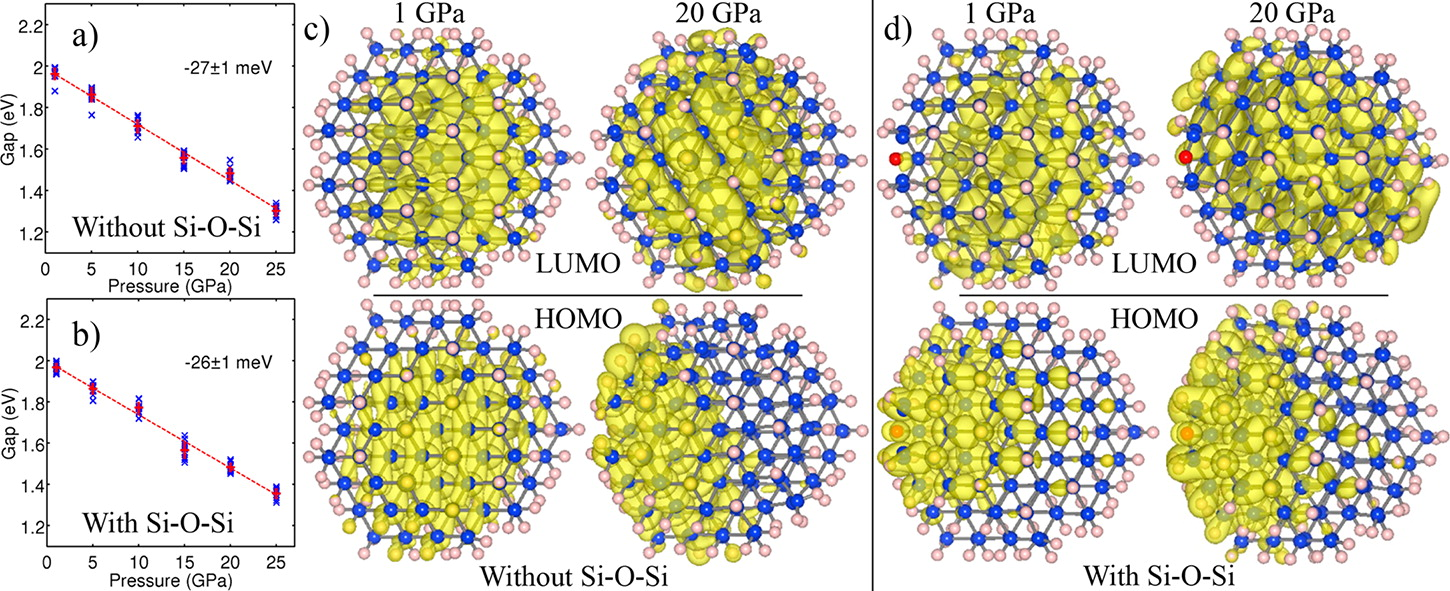
\includegraphics[width=\textwidth]{./Chapter6/sipressure5.jpeg}
\caption[Pressure-dependent energy gap of Si NPs derived from density functional theory.]{Pressure dependence of the HOMO-LUMO energy gap in a 2 nm diameter model H-passivated Si NP (a) without and (b) with a surface defect group (Si-O-Si). At any given pressure, blue crosses ($\times$) denote the HOMO-LUMO gaps for the NP at different steps in the MD trajectory, while the red plus symbol (+) denotes the mean gap. The red dashed line is a linear fit to the mean gaps with the indicated slope. HOMOs and LUMOs for the model Si NP under hydrostatic pressures of 1 and 20 GPa for the NP (c) without and (d) with a surface defect group (Si-O-Si).}
\label{f:sipressure5}
\end{center}
\end{figure}

\subsubsection{Conclusions}
In conclusion, we used pressure to investigate the origin of efficient PL in alkane-terminated, plasma-synthesized Si NPs. We showed that both the bulk modulus and PL emission feature of the investigated NPs shift in step with the bulk crystalline material. These findings strongly suggest that the bright emission from these alkane-terminated Si NPs originates from the X-to-$\Gamma$ transition with insignificant mixing from other bands in the size-range examined. Overall, the indirect-gap character present in the bulk phase remains dominant despite the expectation of relaxation between carrier energy and momentum as quantum-confinement imparts discretization of DOS. The radiative recombination from core-states remains long-lived despite the up to 38\% contribution from quantum confinement to the overall NP emission energy examined here. Finally, because the efficient PL originates from the core states in these structures, our results suggest that optimization of the emission quantum yield from Si NPs, like many other compositions, relies upon surface passivation with ligands that lack density of states within the energy gap rather than decoration of the surface with efficiently emitting surface traps.

\subsection{In Silicon Nanoparticles, Ultrafast Visible-Light Photoluminescence Arises from a Ubiquitous Amorphous Shell}
As noted above, nano-sized Si often exhibits 10\% or greater quantum yield with reported decay components spanning microsecond to picosecond time scales \cite{PhysRevLett.100.067401,de2010red,english2002size,kusova2010brightly,groenewegen2010excited,PhysRevB.49.16845,PhysRevLett.88.097401,godefroo2008classification,PhysRevB.84.085321,dohnalova2013surface}. However, despite numerous studies, disagreement exists regarding the origin of both the fast and slow decay processes. The 650-1000 nm PL feature (termed throughout this section as the “red” feature) displays a microsecond lifetime, and was found in the previous section to originate from indirect gap (X$_{\mathrm{conduction}}$-to-$\Gamma_{\mathrm{valence}}$) recombination.  In this section, we focus on characterization of the radiative recombination that occurs in the 400 to 600 nm energy range, referred to herein as the “blue” feature. \par

Significant excitement exists with regard to multiple reports of fast (nanosecond to subnanosecond) 400 to 600 nm (2-3 eV) PL decay features in Si NPs \cite{PhysRevLett.100.067401,de2010red,dohnalova2013surface,tsybeskov1994blue,valenta2008origin}. Observations of such blue emission, which appear for both Si NPs produced \emph{via} wet chemical synthesis \cite{yang1999synthesis,holmes2001highly}, as well as for plasma-grown materials \cite{PhysRevLett.100.067401} are often attributed to emergent direct gap optical transitions \cite{PhysRevLett.100.067401,de2010red,valenta2008origin} that may arise from at least two possible mechanisms. First, the bulk semiconductor requirement of carrier energy and linear momentum conservation can become less stringent upon quantum-confinement owing to replacement of electronic band structure with discrete electronic states, in similarity to molecules \cite{PhysRevLett.101.217401,PhysRevLett.75.3728}. In addition, during the time that a photoexcited electron and hole (an exciton) collectively exceed the lowest energy “band-edge” transitions ($\sim$1 ps in most semiconductor nanomaterial compositions) \cite{PhysRevLett.80.4028,PhysRevLett.95.196401}, radiative recombination can occur between states that possess the same momentum and do not necessitate involvement of a momentum-conserving phonon \cite{de2010red}. Observation of such “phononless” emission from hot exciton states requires either large oscillator strength or slowed cooling of hot excitons. \par

A recent report utilized time-resolved PL spectroscopy and a quasi-continuous sample re-excitation scheme in order to accentuate and spectrally characterize blue emission features, but lacked sufficient time-resolution to directly characterize the time scale of the recombination process \cite{de2010red}. An additional study also suggested that direct-gap transitions may arise in colloidally prepared, alkyl-terminated NPs owing to modification of the electronic structure by covalent surface functionalization \cite{dohnalova2013surface}. In this case, 400-600 nm emission does not compete with intraband relaxation, but instead, hybridization with the covalently attached surface ligands purportedly modifies the band-edge electronic wave functions such that substantial broadening of the related $k$-space distribution occurs, permitting direct recombination at the $\Gamma$-point. That report concludes that high-energy emission stems from recombination produced within the Si NPs rather than from defect states, but the dynamics of the obtained PL spectra were not characterized with sufficient time-resolution to distinguish processes related to carrier thermalization. \par

Here, we examine multiple sizes and degrees of crystallinity of plasma-synthesized colloidal Si NPs using a previously reported synthetic method \cite{PhysRevB.80.115407} with a focus on emission in the 400-600 nm “blue” spectral region. We spectrally and, for the first time, temporally resolve PL from the particles with up to single-picosecond time resolution. From these measurements we observe a $\sim$30 ps decay component as the fastest PL relaxation time scale. This spectral and temporal resolution allows us to definitively assign lifetimes to the observed PL features. Based on our observations, we suggest that the blue PL band in Si NPs originates from an amorphous component in the samples and that the rapid emission processes are too slow to be consistent with a hot exciton radiative process. We also show through MD (MD) simulations that experimental Raman spectra obtained at different plasma powers are well-described by particles presenting a thin, amorphous surface (consistent with electron microscopy) which we suggest gives rise to the fast emission.

\subsubsection{Transient Photoluminescence Experiments}
Alkyl-passivated Si NPs fabricated using the synthesis method detailed above and in the work by Mangolini \emph{et al.} \cite{mangolini2007plasma} were suspended in octane and loaded into an airtight cuvette under a nitrogen atmosphere. The room-temperature NPs were photoexcited with 35 fs pulses from a 2 kHz amplified Ti-sapphire laser at 325 nm (3.8 eV). Excitation fluence sufficient to ensure single exciton dynamics ($N_{exc} << 1$) was utilized. PL photons were directed to a 150 mm spectrograph and single-photon-sensitive streak camera. Detector regions were binned vertically or horizontally to produce time-resolved spectra or spectrally resolved dynamics, respectively. It is important to note that the time resolution of a streak camera inherently depends on the observation window. Longer observation windows necessarily yield reduced temporal resolution, and vice versa. Therefore, dynamics which appear well-resolved by a streak camera utilizing a 120 ps observation window can appear instrumentally limited when examined using longer observation windows.

\subsubsection{Ultrafast Photoluminescence Dynamics of Highly Crystalline Silicon (c-Si) Nanoparticles}
Crystalline Si-NPs were synthesized in a radio frequency (RF) plasma (80 W) and covalently functionalized with 1-dodecane using the methods described above. Single-exciton PL dynamics under ambient conditions were examined using a streak camera, which provides simultaneous spectral and temporal resolution as described above. Figure \ref{f:amsi1} (left panel) depicts a streak camera image of PL recorded for the first 10 ns following photoexcitation of an ensemble of 3.2 nm-diameter crystalline Si (c-Si) NPs. The top right panel of Figure \ref{f:amsi1} shows a late-time PL spectrum (temporally integrated from 9-10 ns), which reveals two clear contributions: a blue PL band centered near 450 nm and a red PL band centered at 700 nm. The presence of distinct blue and red bands is consistent with many previous reports \cite{PhysRevLett.100.067401,tsybeskov1994blue,valenta2008origin,yang1999synthesis,holmes2001highly}, although their origins remain disputed. PL immediately following the excitation pulse (integrated from 0-1 ns, shown in the bottom right panel of Figure \ref{f:amsi1}) reveals a third PL band intermediate in energy, termed the “green” feature. Such a green feature was reported by de Boer \emph{et al.}, who attributed it to phononless radiative recombination of hot excitons, despite a lack of direct dynamical characterization \cite{de2010red}. \par

\begin{figure}
\begin{center}
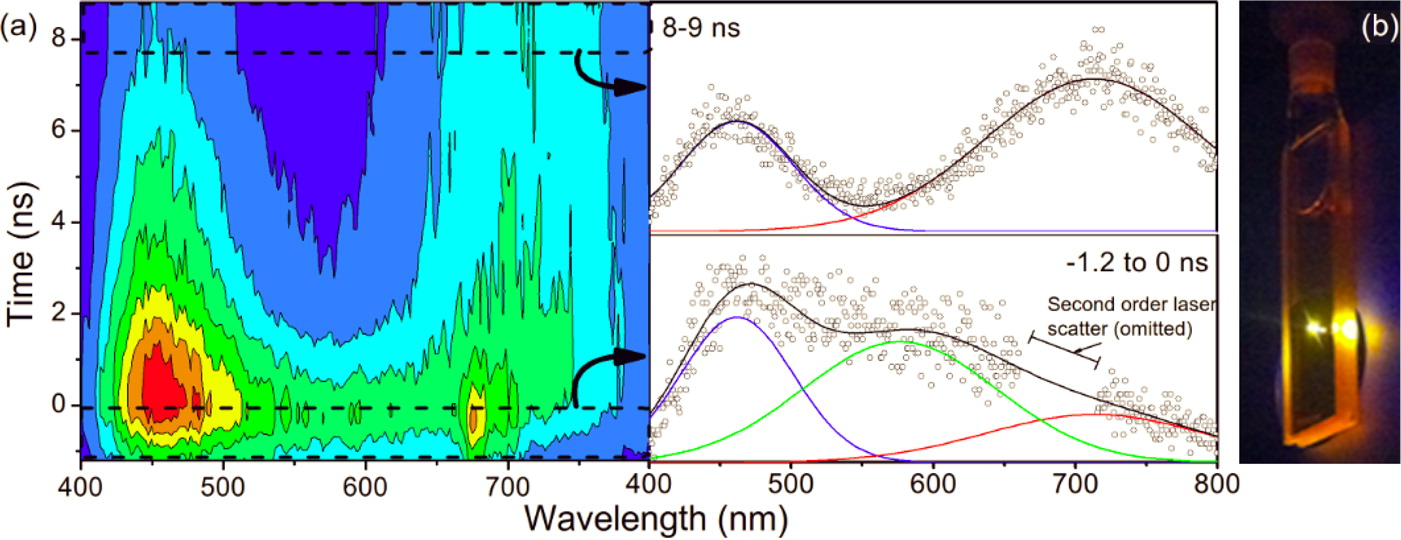
\includegraphics[width=\textwidth]{./Chapter6/amsi1.jpeg}
\caption[Nanosecond-scale evolution of PL from crystalline Si nanoparticles.]{(a) A streak camera image for crystalline 3.2 nm diameter Si NPs photoexcited at 325 nm (3.8 eV). Dynamics over a 10 ns time window subsequent to photoexcitation are shown. The apparent buildup of PL prior to $t = 0$ is related to an instrumentally limited response. The panels on the right side show PL spectra integrated temporally over the regions indicated by the dotted lines and arrows in the left panel (top right panel: PL spectra from 9-10 ns, bottom right panel: 0-1 ns). Solid lines in the right panels indicate Gaussian lineshapes used to fit the PL spectra. The peak centers and line widths obtained from the fits in the 9-10 ns spectra were fixed and used in the fitting of the 0-1 ns spectra, a procedure justified by the absence of temporal evolution in the PL line width. In the bottom right panel, data points from 650-700 nm are contaminated by second order scatter from the 325 nm excitation source; these points are omitted from the plot and the Gaussian fitting procedure. (b) A photo showing PL from 3.2 nm diameter Si NPs.}
\label{f:amsi1}
\end{center}
\end{figure}

To investigate the fast dynamics of these features we examined PL using single-picosecond temporal resolution streak camera electronics. Such high time resolution measurements applied to a broadband emitter necessitate the use of bandpass spectral filtering in order to obtain wavelength-resolved dynamics free from artifacts. Figure \ref{f:amsi2}(a) depicts a streak camera image of PL from the same ensemble of 3.2 nm diameter c-Si NPs for 100 ps following photoexcitation. Because of required filtering optics, only the high-energy shoulder of the red PL band is observed and the high-energy edge of the blue PL band is also truncated. Truncation due to filtering optics is indicated in Figure \ref{f:amsi2}(a). The red feature exhibits a microsecond decay lifetime and is present in this data as a persistent shelf. The blue feature, however, exhibits decay on this time scale; this is evident in the time-resolved spectra displayed in Figure \ref{f:amsi2}(b) for the same sample. Notably, aside from decreasing intensity with time, the spectra exhibited little temporal evolution in terms of both energy and spectral profile. For all c-Si NP sizes studied, the PL spectral profile remains relatively constant for 800 ps following photoexcitation. Importantly, the consistent PL profile at blue wavelengths suggests that the decay in PL intensity is due to the collective depletion of a single population of emitters. We explore the blue feature dynamics further in Figure \ref{f:amsi2}(c), which displays PL intensity at 500 nm as a function of time for the same sample. Comparison to the instrument response function (IRF, also shown in Figure \ref{f:amsi2}(c)) obtained from examination of pump laser scatter indicates that the blue feature decay is well-resolved at these time scales and that no faster dynamics are taking place in the system with significant amplitude. Fitting the dynamics in Figure \ref{f:amsi2}(c) to a monoexponential decay function yields a time constant of 28 ps. At slightly longer times, a subnanosecond decay component is also observed. Fitting the dynamics from 0 to 800 ps to a biexponential decay function yields time constants corresponding to the $\sim$30 ps feature discussed above and a component having a lifetime that is consistently hundreds of picoseconds (see Table \ref{table:amsiT1} for fitting results and Appendix C for PL dynamics from 0-800 ps). \par

\begin{figure}
\begin{center}
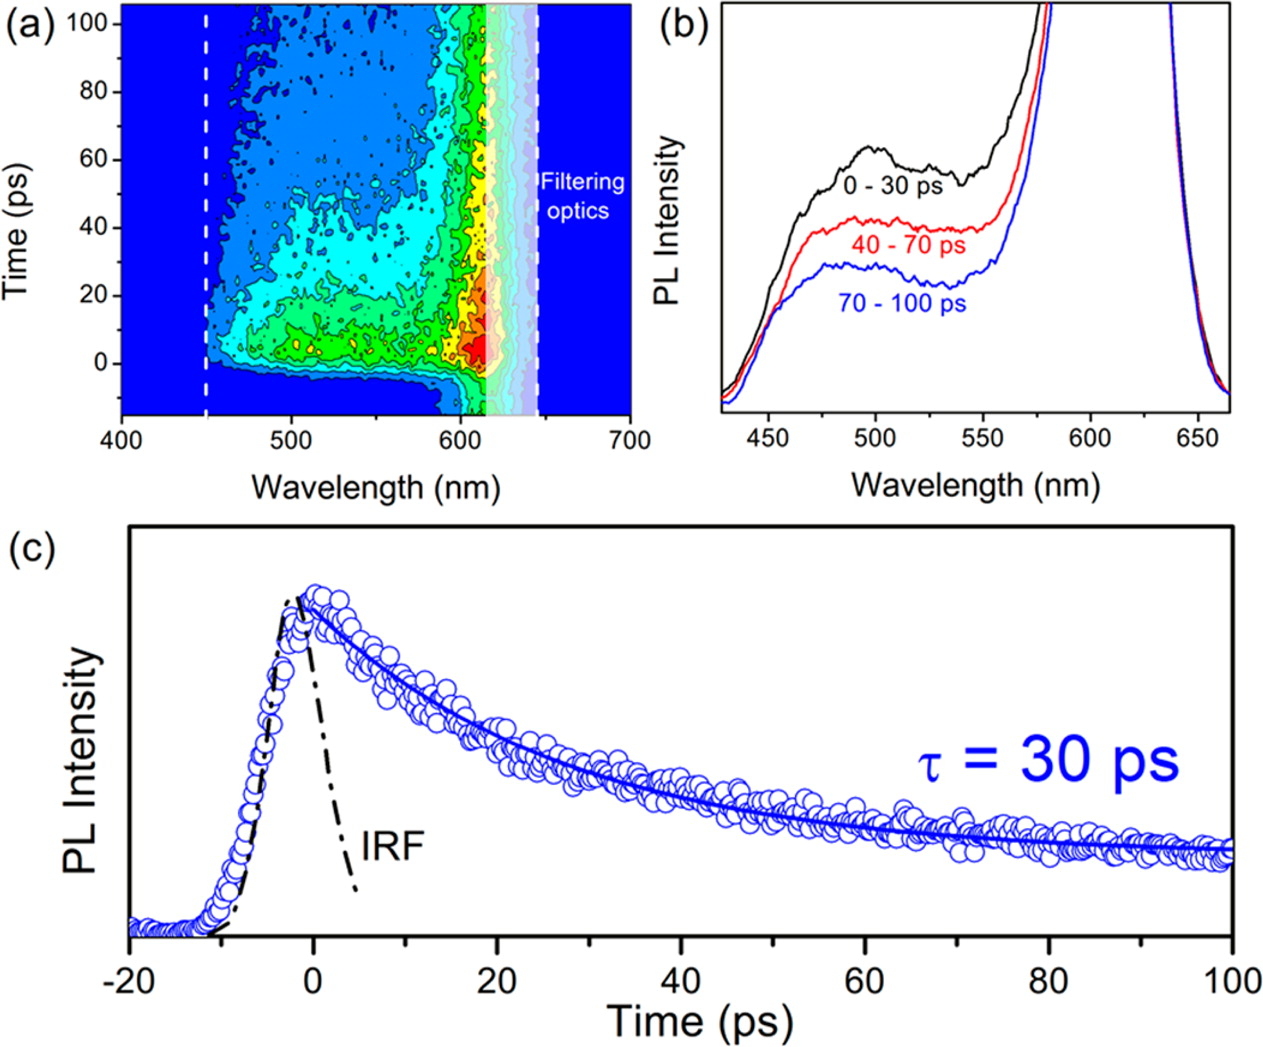
\includegraphics[width=0.75\textwidth]{./Chapter6/amsi2.jpeg}
\caption[Picosecond-scale evolution of PL from crystalline Si nanoparticles.]{(a) Streak camera image of PL from the 3.2 nm diameter Si NPs recorded for 100 ps following photoexcitation. Necessary filtering optics and sample reabsorptions artificially truncate the PL spectrum on the red and blue edges. Truncation due to band-pass filtering is indicated by dashed white lines, while the translucent white shading indicates regions where signal is attenuated by the filtering optics, but not completely blocked. The high-energy tail of the red PL band is apparent as a long-lived shelf, as it does not fully relax prior to re-streaking of the time-resolving detector. (b) Main panel: Time-resolved PL spectra in three different temporal regions for the same sample. Temporally binned regions are indicated by labels. (c) Time-resolved PL dynamics spectrally integrated from 475 to 525 nm. The solid blue line indicates a fit of the dynamics to a single exponential decay function. The instrument response function (IRF) is indicated by a dotted black line. Note that this IRF corresponds only to a streak camera observation window of 120 ps.}
\label{f:amsi2}
\end{center}
\end{figure}

\begin{table}
\caption{Time Constants for the Biexponential Decay Observed in the PL Dynamics for the First 800 ps Following Photoexcitation of 4 Silicon NP Sizes.$^a$}
\centering
\begin{tabular}{c r r }
\hline\hline
Diameter (nm) & $\tau_1$ (ps) & $\tau_2$ (ps) \\
\hline
2.6 & 27.8 $\pm$ 0.6 & 204 $\pm$ 7 \\
3.2 & 26 $\pm$ 4 & 243 $\pm$ 12 \\
3.8 & 16 $\pm$ 1 & 195 $\pm$ 13 \\
4.6 & 26 $\pm$ 7 & 563 $\pm$ 47 \\
\hline
\end{tabular} \par
\bigskip
$^a$ Errors are derived from the fitting function.
\label{table:amsiT1}
\end{table}

Notably, picosecond scale dynamics do not reveal distinct blue and green decay components, indicating that the green feature noted in Figure \ref{f:amsi1} displays dynamics that are indistinguishable from the blue feature on picosecond time scales, and that no spectral range exhibits decay dynamics having a time constant faster than $\sim$20 ps.

\subsubsection{Characterization of Amorphous Silicon Nanoparticles}
In addition to highly crystalline particles, we examined reduced crystallinity Si NPs produced using lower plasma power as described and characterized in depth in recent reports \cite{PhysRevB.80.115407,anthony2011routes}. Noting numerous reports of visible PL from amorphous silicon structures \cite{pankove1977PL, wang2003high,wehrspohn1997electrochemistry}, we systematically investigated the role of lattice crystallinity on PL spectrum. Figure \ref{f:amsi3}(a) depicts Raman scattering collected from Si NPs synthesized at plasma powers of 8, 30, 45, and 60 W. NPs synthesized at higher powers clearly yield more narrow Raman scattering spectra, consistent with higher crystallinity samples. The NPs synthesized at 8 W exhibit a broad, featureless peak, corresponding to an entirely amorphous sample \cite{PhysRevB.80.115407}. We also present the Raman scattering spectrum of bulk crystalline Si, which exhibits a sharp peak at 520 cm$^{-1}$ corresponding to the transverse optical (TO) phonon mode. This peak is also clearly present in the Si NP Raman scattering spectra, along with a low-frequency shoulder, the presence of which has been correlated with amorphous materials \cite{duan2012raman}. The relative intensity of the low-frequency shoulder appears to be larger for lower plasma powers.

\begin{figure}
\begin{center}
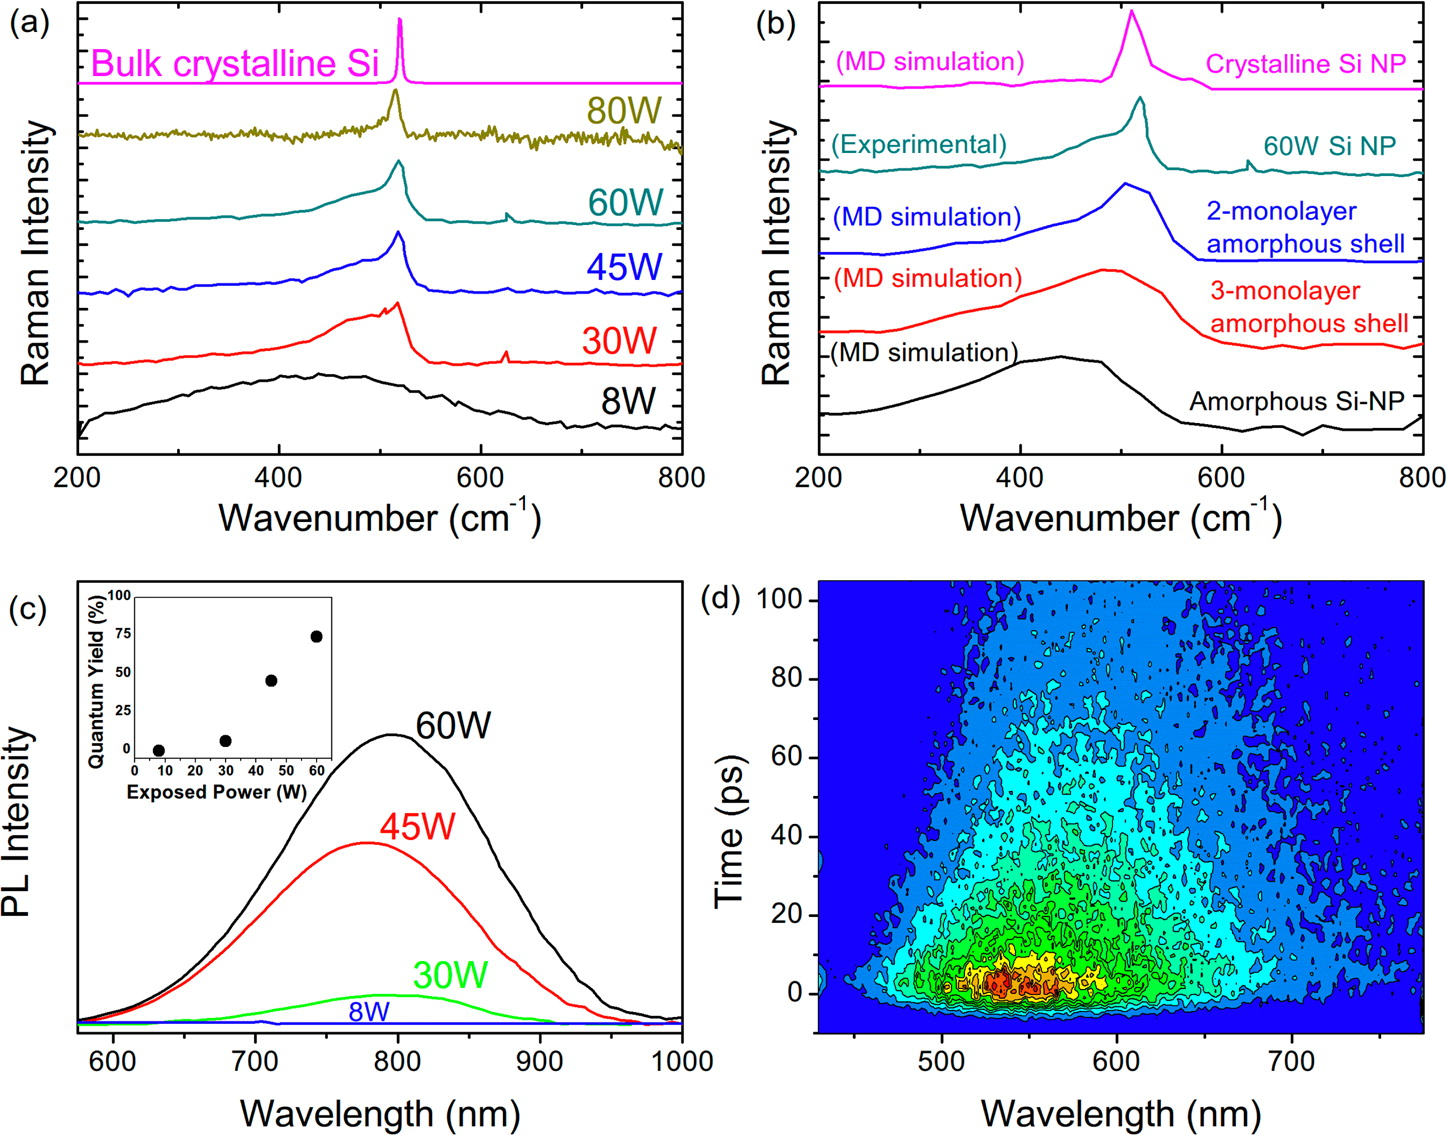
\includegraphics[width=0.75\textwidth]{./Chapter6/amsi3.jpeg}
\caption[Raman scattering and PL from Si NPs synthesized at a variety of powers.]{(a) Raman scattering spectrum of Si NPs synthesized at the indicated plasma powers. The peak at 500 cm$^{-1}$ is attributed to the transverse optical (TO) phonon and diminishes in intensity for samples synthesized at lower powers (less crystalline). The Raman scattering spectrum of bulk crystalline Si is also displayed. All Raman spectra have been mathematically normalized and plotted with a vertical offset. (b) Raman scattering spectra for Si NPs predicted from MD simulations as described in the Appendix. Color-coded data is shown for a fully crystalline particle, particles with 2 or 3 monolayers of amorphous Si on their surfaces, and a fully amorphous particle. The experimental data for Si NPs synthesized at 60 W from (a) is reproduced here for comparison. (c) PL spectra of Si NPs synthesized at four different plasma powers (indicated on the figure). Higher plasma powers nominally yield more crystalline samples. Inset: PL quantum yield for Si NPs as a function of the plasma power used during their synthesis. (d) A streak camera image of PL from Si NPs synthesized at a plasma power of 8 W (e.g., fully amorphous Si). Photoexcitation energy was 3.8 eV.}
\label{f:amsi3}
\end{center}
\end{figure}

To gain a clearer understanding of the correspondence between Raman spectra, sample crystallinity, and address the potential coexistence of crystalline and amorphous phases, we performed MD simulations of experimentally sized (4 nm diameter) Si NPs that present varying amounts of amorphous material on the surface. The construction of particles presenting an amorphous surface was motivated by the clear presence of a disordered surface layer in transmission electron microscopy (TEM) images of Si NPs in addition to the presence of stretching modes in the infrared absorption spectrum (see Appendix C) which are attributed to undercoordinated Si species (SiH$_2$ and SiH$_3$). Using force constants obtained from a relaxation of interatomic forces in the structures, we computed expected Raman scattering spectra. The details of amorphous structure generation, MD simulations, and Raman scattering calculations can be found in Appendix D.  Figure \ref{f:amsi3}(b) displays the MD-derived Raman scattering spectra for four particles: A fully crystalline particle, particles with either 2 or 3 monolayers of amorphous material on the surface and an entirely amorphous particle. These simulations suggest that increasing amounts of amorphous material on crystalline core give rise to a lower-frequency shoulder near the TO feature. The experimental Raman scattering for Si NPs synthesized at 60 W (Figure \ref{f:amsi3}(a)) is also reproduced on this graph for comparison. The calculated Raman spectrum of the entirely crystalline Si NP lacks good agreement with experimental data. Notably, however, the calculated Raman spectrum for a particle presenting a 2-monolayer amorphous Si shell closely replicates the experimental spectrum. Asymmetric broadening of the TO peak in the presence of amorphous material was previously reported by Duan \emph{et al.} In analysis of Raman scattering from matrix-embedded Si nanocrystals, they attribute a similar low-frequency shoulder to amorphous material but do not comment further on the origin or character of such material\cite{duan2012raman}. Additionally, a comparison of TEM to Raman-based NP sizing methods lead Ristić and co-workers to suggest that a shell of amorphous material could explain the observed discrepancies in the NP sizes obtained \cite{ristic2009application}. The persistence of a disordered surface, even in the absence of organic ligands, led to a similar suggestion by Panthani \emph{et al} \cite{panthani2012graphene}. The Raman spectrum of nanocrystalline Si, in conjunction with the Raman spectrum of purely amorphous Si, can be used to estimate the relative amounts of amorphous and crystalline material \cite{smit2003determining}. In brief, the ratio of crystalline and amorphous TO phonon peak areas, with appropriate scaling, reflects the fraction of crystalline material in the sample. By applying the method put forth in the work of Smit \emph{et al.} \cite{smit2003determining} to our Si NPs, we find that the 8, 30, 45, 60, and 80 W samples contain 100, 62, 57, 48, and 35\% of entirely amorphous material, respectively (see Appendix C for fitting procedure details). \par 

The static PL spectra of the Si NPs studied here are dominated by broad emission corresponding to the red (indirect-gap) PL band for all plasma-synthesis powers, as shown in Figure \ref{f:amsi3}(c). Quantum yield clearly increases with increasing plasma powers (Figure \ref{f:amsi3}(c), inset). Figure \ref{f:amsi3}(d) depicts a streak camera image of PL from an ensemble of Si NPs synthesized at 8 W (least crystalline) for 100 ps following photoexcitation. A single strong emission band is evident, centered roughly at 550 nm. Comparisons of the PL decay shown in Figure \ref{f:amsi3}(c) to the PL rise and IRF indicates that these dynamics are well-resolved and that no faster processes occur. \par

Next, we compare c-Si NPs and amorphous silicon nanoparticles (a-Si NPs). The spectral profile of the initial PL amplitude (integrated temporally from 0-100 ps following photoexcitation) for 4 nm diameter a-Si NPs shows a systematic dependence on plasma power, as depicted in Figure \ref{f:amsi4}(a). Figure \ref{f:amsi4}(a) shows normalized PL spectra temporally integrated from 0-100 ps for our most and least crystalline samples. a-Si NPs produced using low power (8 W) show a broad PL band centered at $\sim$550 nm. The Si NPs made at higher plasma power (60 W) continue to produce blue PL but also exhibit increased red PL intensity, the high energy shoulder of which is evident in Figure \ref{f:amsi4}(a) (required filtering optics truncate the majority of the red emission band, as indicated in Figure \ref{f:amsi2}(a)). Given that all four samples exhibit similar size and organic ligand termination, the data in Figure \ref{f:amsi4}(a), which have been normalized for comparison of spectral profiles, strongly suggest that the observed differences in PL spectra are related to the extent of Si NP crystallinity. In light of this, we attribute blue-feature PL to emission from remnant amorphous material in the Si NP ensemble, which we suggest is present as a shell of amorphous material. With higher plasma power, the relative amount of amorphous material decreases as more crystalline NPs are produced (Figure \ref{f:amsi3}(b)), whereupon long-lived, indirect-gap excitonic (red-feature) PL dominates the emission spectrum (Figure \ref{f:amsi4}(a)) at every time range. \par

\begin{figure}
\begin{center}
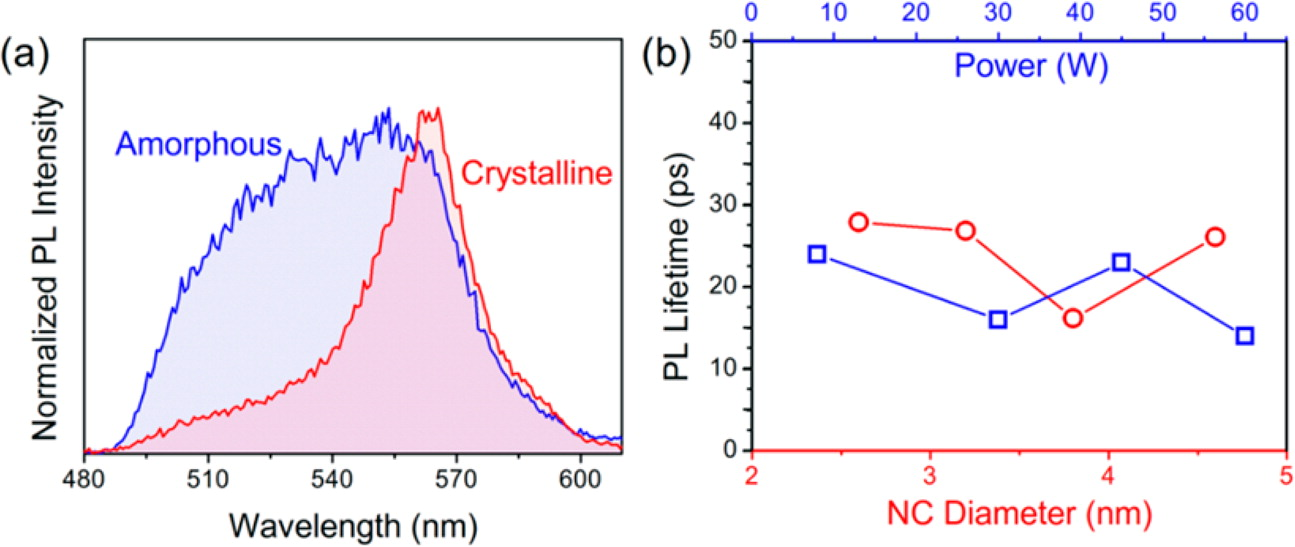
\includegraphics[width=\textwidth]{./Chapter6/amsi4.jpeg}
\caption[Comparison of PL from crystalline and amorphous Si NPs.]{(a) Mathematically normalized PL spectra temporally binned from 0-100 ps following photoexcitation for Si NPs synthesized for amorphous (8 W) and crystalline (60 W) Si NPs, which are indicated on the figure. Although filtering optics artificially truncate the red edge of the PL spectrum, the same optics were used in collection of both PL spectra displayed. (b) Lifetime of the fastest dynamics observed for all of the samples considered in this study. The blue (squares) data and top axis correspond to the Si NPs synthesized at indicated plasma powers, while the red (circles) data and bottom axis correspond to four sizes of highly crystalline Si NPs.}
\label{f:amsi4}
\end{center}
\end{figure}

We aim to resolve the origin of blue PL photons emitted from Si NPs as well as the processes responsible for the decay of the associated PL band (the blue feature). Regarding the dynamics of the blue PL feature, we note that the NP size-independent fastest PL decay of $\sim$30 ps is an order of magnitude slower than typical intraband relaxation time in quantum-confined materials \cite{PhysRevLett.80.4028,PhysRevLett.95.196401}, a process with which phononless PL would be competitive. Conversely, if indeed the rapid PL decay were associated with hot carrier recombination, it would imply the slowest intraband relaxation time ever reported for core-only colloidal NPs. Furthermore, the red PL feature, which we recently established arises from lowest-energy exciton states within the NP core \cite{hannah2012origin}, does not exhibit a rise time that correlates with the “green” feature decay (as observable at 525 nm in Figure \ref{f:amsi2}(a)), consistent with ultrafast (1 ps or less) relaxation of hot excitons as found in numerous other semiconductor NPs \cite{PhysRevLett.80.4028,PhysRevLett.95.196401}. This lack of a correlated rise time offers additional evidence that the $\sim$30 ps decay does not represent a hot exciton radiative process. \par

Instead, we posit that the $\sim$30 ps decay feature arises from a nonradiative process associated with amorphous material. Indeed, if a radiative process were responsible, the biexponential dynamics would imply two separate populations of emitters with different associated PL line widths. Given the unchanging PL profile (Figure \ref{f:amsi2}(b)), it is unlikely that biexponential dynamics arise from two separate radiating populations. This notion is further supported by the absence of a strong optical absorption transition in this spectral region \cite{gresback2011combined}. Considering the oscillator strength, which would be associated with such a rapid radiative transition, it is highly unlikely that a 30 ps decay (which represents the upper bound of our lifetime measurements) caused by optical transitions would have no apparent manifestation in the optical absorption spectrum of the Si NPs. Fermi's Golden Rule allows us to relate the optical radiative rate ($\tau_{PL}^{-1}$) to the optical transition matrix element $|\left\langle\Psi_1|\vec{p}|\Psi_0\right\rangle|^2$ \emph{via} Eq. \ref{eq:amsi1}:

\begin{equation}\label{eq:amsi1}
\tau_{PL}^{-1} = \frac{e^2n\omega}{\pi\varepsilon_0m^2\hbar c^3}|\left\langle\Psi_1|\vec{p}|\Psi_0\right\rangle|^2
\end{equation}

In Eq. \ref{eq:amsi1}, $e$ is the fundamental charge, $n$ is the refractive index, $\hbar\omega$ is the emission energy, $\varepsilon_0$ is the vacuum permittivity, $m$ is the electron mass, and $c$ is the speed of light in vacuum.  Coupled with the expression for oscillator strength ($f = (2/\hbar m\omega)|\left\langle\Psi_1|\vec{p}|\Psi_0\right\rangle|^2$), we can express the oscillator strength of a given transition in terms of radiative lifetime, as shown in Eq. \ref{eq:amsi2}:

\begin{equation}\label{eq:amsi2}
f = \frac{2\pi\varepsilon_0mc^3}{e^2n\omega^2}\frac{1}{\tau_{PL}}
\end{equation}

For the 30 ps decay ($\hbar\omega = 2.75$ eV, $\tau_{PL}$ = 30 ps), a radiative transition would be associated with an oscillator strength of $f = 13.8$.  By comparison, the long-lived red PL ($\hbar\omega = 1.75$ eV, $\tau_{PL} = 75$ $\mu$s) has an oscillator strength of $f = 1.3 \times 10^{-5}$, which is several orders of magnitude smaller. Provided that significant silicon atom rearrangements do not occur in the excited state, the absence of a strong optical transition near 450 nm in the absorption spectrum taken together with the constant PL line width (Figure \ref{f:amsi2}(b)) strongly suggest that radiative recombination cannot account for the $\sim$30 ps decay observed here. \par

Recently, Dohnalova and co-workers suggested an intrinsic origin to the blue band observed for alkyl-terminated Si NPs prepared \emph{via} a wet chemical synthesis \cite{dohnalova2013surface}. For these NPs, they report primarily blue PL and an absence of red emission, suggesting that the blue band is not related to hot exciton emission (a scenario in which one would expect to see blue and band-edge red PL). Following intense laser irradiation they observe an increase of red PL, which they attribute to sample oxidation. However, their results may also be interpreted in the context of our work as arising from changes in sample crystallinity. The wet chemical synthesis used in the study by Dohnalova \emph{et al.} may not have provided sufficient energy to form c-Si, a covalently bonded material. Upon laser irradiation, we suggest that sample annealing occurs, increasing the amount of crystalline material present and, consequently, the relative intensity of the red PL, which we and others attribute to indirect gap, band-edge recombination. Similarly, a recent study by Dasog and co-workers found that Si NPs synthesized at higher temperatures exhibited red, indirect gap PL, while Si NPs synthesized \emph{via} more mild colloidal routes yielded rapid, blue PL \cite{dasog2013chemical}. These results, taken in conjunction with our presented data, lead us to the conclusion that high-energy PL is a result of emission arising from amorphous material. The persistence of amorphous material even in our most crystalline samples is supported by near-exact agreement between experimental Raman scattering spectra for c-Si NPs and theoretical Raman spectra calculated for crystalline core particles covered by a two-monolayer amorphous shell. The presence of amorphous material in the form of a persistent shell is supported by our observation of a disordered surface layer in TEM images as well as the presence of SiHi$_3$ and SiH$_2$ on the NP surface (see Appendix C). \par

In addition to the spectral similarities noted above for amorphous Si NPs and the blue feature observed in crystalline Si NPs, we find that PL dynamics for amorphous Si strongly resemble those found for the blue feature in crystalline Si. Indeed, regardless of sample size or crystallinity, we find the fastest PL decay observed to have a time constant of $\sim$30 ps. This is depicted in Figure \ref{f:amsi4}(b), which shows the fitted time constant obtained for the fastest decay in the system for each sample considered in this study. The similarity and time scale of these dynamics suggests that in all cases, rapid PL decay is caused by the same (nonradiative) process. Furthermore, the longer component of the blue PL decay, for each power used, has a fitted time constant between 150 and 200 ps, very similar to the highly crystalline Si NPs studied in this work (Table 1). The rapid decay process we observe in completely amorphous (8 W) Si NPs is likely hole trapping in the strained regions of the amorphous network. This type of trapping was suggested in recent theoretical works by Lajoie \emph{et al}. \cite{lajoie2010optical} and Wagner \emph{et al.} \cite{wagner2008microscopic}. Given that a multitude of characterization methods (TEM, FTIR, Raman) indicate that highly crystalline particles still present an amorphous surface layer, we suggest that hole trapping processes occur in this thin amorphous shell. \par

\subsubsection{Conclusions}
Overall, we have identified and resolved, in the energy and time domains, a high energy (400-600 nm) band in the PL spectrum of plasma-synthesized, covalently functionalized Si NPs. Our findings constitute a comprehensive examination of the ultrafast dynamics of the 400-to-600 nm PL band previously attributed to both defect-related recombination and phononless PL in Si NPs. Whereas previous reports noted instrumentation-limited decay features, we examine these features with instruments having a response time adequate to resolve them. This new information allows us to resolve long-standing controversies regarding the fast PL band in quantum confined Si and conclusively attribute observed dynamics to a nonradiative decay process which we suggest is hole trapping in a persistent surface layer of amorphous Si. For the first time, we also examine the role of core crystallinity in PL. These results shed light on the origin of high energy PL in Si NPs and also provide an explanation for the observation of this PL in a wide variety of Si NP preparations, as they do not invoke surface chemistry or pseudodirect gap recombination. We expect that our work will stimulate future experimental and theoretical efforts regarding the role of lattice disorder in the optical properties of silicon nanomaterials. Furthermore, these findings present an opportunity for the systematic tailoring of absorption and emission spectra \emph{via} core crystallinity, providing an additional degree of tunability to this technologically important class of materials.

\chapter{Pressure-Induced Structural Changes in Semiconductor Nanocrystals}

\section{Introduction}

While studies of NCs subject to applied pressure were initially undertaken with the aim of understanding the pressure dependence of properties such as the NC energy gap, the group-IV (in particular, Si and Ge) NCs studied during the course of this dissertation research exhibit pressure-dependent structural behvaior that is sufficiently interesting to warrant its own discussion. \par
Nanocrystals are smaller than the domains involved in solid-solid transformations exhibited by bulk materials. Furthermore, they generally exhibit defect-free cores and experience pressure-induced phase transitions as a result of only a single nucleation event \cite{PhysRevLett.76.4384}. In general, phase transitions cause a shape change in the NC from having low-index, low-energy surfaces (as synthesized in the low-pressure phase) to high-index, high-energy surfaces. Furthermore, they lack internal defects to serve as nucleation sites. Taken together, these two factors generally cause NCs to exhibit elevated phase transition pressures relative to the bulk phase \cite{PhysRevLett.76.4384, tolbert1994size}.\par
While the high-pressure phases of larger SiO$_2$ passivated Si NCs have been studied previously, the NCs studied here result from plasma or colloidal synthesis methods and experience covalent alkyl termination. Furthermore, the NCs studied here are much smaller and strongly quantum confined. Given the different surface chemistry, smaller size, and quantized electronic structure, it is worth studying the pressure-dependent behavior of these materials. In this chapter we present experimental and computational studies of pressure-induced structural changes in Si and Ge NCs having covalent termination and extremely small sizes (diameter $<$ 4 nm). Experimental characterization of pressure-dependent NC structure using XRD reveals elevated phase transition pressures and a compressibility nearly identical to the bulk phase for both Si and Ge NCs. Simulations of the pressurization experiment using MD show good agreement between experimental and MD-derived NC structures. Analysis of the phase transition mechansism \emph{via} an ordering parameter reveals that a majority of atoms experience a phase transition at the same time. We suggest that this behavior may be related to anomalously similar compressibility of group-IV NCs to the bulk phase.
\section{Structural Characterization of Si and Ge Nanocrystals Under Applied Hydrostatic Pressure}
\subsection{Silicon Nanocrystals}
We investigated the room-temperature pressure-dependent structure of colloidal Si NCs in the pressure range from ambient up to $\sim$73 GPa. One formative study on the subject is available for comparison. In 1996, Tolbert \emph{et al.} conducted pressure-dependent XRD on 9.6 and 49 nm diameter flame-pyrolysis-derived, SiO$_2$-coated Si NCs in an effort to characterize the effect of nanoparticle size on phase transition pressures \cite{PhysRevLett.76.4384}. Measurements on 9.6 nm NCs revealed elevated phase transformation of the semiconducting Si(I) to a metallic phase near 22 GPa and loss of the metallic phase upon pressure release. XRD experiments on 49.2 nm NCs revealed transformation of Si(I) to the Si(V) phase (phases described in some more detail below) between 17 and 21 GPa. Upon partial reduction of pressure, Si(XI) and Si(II) phases were observed. Full decompression showed transformation of the NCs into a-Si. \par

Specifically, we performed pressure-dependent XRD measurements in order to both obtain the unknown compressibility of the NCs, which for binary ionic semiconductors deviates significantly from bulk values \cite{PhysRevLett.101.217401} as well as to investigate phase transition pressures for nonoxide-coated nanoparticles. Samples were loaded into diamond anvil cells as described in Chapter 6. Pressure-dependent XRD measurements were performed at the Advanced Photon Source, Argonne National Laboratory, at beamline 13-ID-D of the GSECARS sector using a 37 keV X-ray beam focused to a 4 $\mu$m diameter spot. X-ray fluence was controlled to avoid sample damage. The distance-to-sample and tilting of a MAR165-CCD X-ray detector was calibrated using a CeO$_2$ standard. \par

While Tolbert found that transition pressures were elevated in earlier XRD work, the NCs studied here are an order of magnitude smaller and organically passivated rather than SiO$_2$ encapsulated, which could substantially modify phase transition pressures. For reference \cite{PhysRevB.41.12021,katzke2007structural,olijnyk1984structural}, bulk Si transforms from the diamond structure (Si(I), $Fd\bar{3}m$) to the β-Sn phase (Si(II), $I4_1/amd$) at approximately 11.7 GPa. The metallic $\beta$-Sn phase then undergoes a transformation to the closely related $Imma$ (Si(XI)) structure at 13.2 GPa. At just a slightly higher pressure of 15.4 GPa, the $Imma$ phase further converts to a primitive hexagonal ($P6/mmm$, or Si(V)) structure. At $\sim$38 GPa, this hexagonal form of Si transforms into an orthorhombic phase Si(VI) ($Cmca$ space group). By 42 GPa, the orthorhombic Si(VI) is again transformed into a hexagonal close-packed form (hcp, Si(VII), $P63/mmc$). Finally, at $\sim$79 GPa, the hcp, Si(VII), transforms into face-centered cubic (fcc) structure (Si(X), $Fm3m$). \par

\begin{figure}
\begin{center}
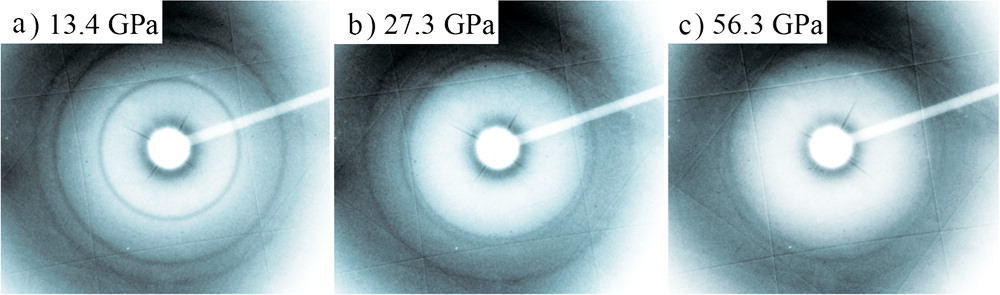
\includegraphics[width=\textwidth]{./chapter7/sipressure2.jpeg}
\caption[Two-dimensional pressure dependent XRD data for Si nanocrystals.]{Raw XRD patterns for a 3.8 nm diameter Si NC sample measured at the indicated pressures.}
\label{f:sipressure2}
\end{center}
\end{figure}

High-quality, two-dimensional pressure-dependent XRD data, such as those shown in Figure \ref{f:sipressure2}, are summarized in Figure \ref{f:sipressure3}. Specifically, Figure \ref{f:sipressure3}(a)-(c) show XRD spectra for multiple sizes of Si NCs at the indicated pressures. Presented spectra are offset vertically both for clarity and to indicate measurement chronology, where pressure reversal is denoted with an “R” preceding the measured pressure. Indexing of the initial, ambient pressure phase of the NCs (Figure \ref{f:sipressure3}(e)) shows a clear fit to the Si(I) phase as expected. Compression of the Si(I) phase appears isotropic and extraction of the unit cell parameters as a function of pressure (Figure \ref{f:sipressure3}(d)) allowed us to calculate the room temperature and zero-pressure bulk modulus (B$_0$) of the different NC samples by fitting the data to third-order Vinet and Birch-Murnaghan (B-M) equations of state (Eqs. \ref{eq:sipressure1} and \ref{eq:sipressure2}, respectively) \cite{fei2007toward}. \par
\begin{equation}\label{eq:sipressure1}
P_{300} = 3B_0\left(\frac{V}{V_0}\right)^{-\frac{2}{3}}\left[1-\left(\frac{V}{V_0}\right)^{\frac{1}{3}}\right]\exp\left\{1.5\left(B_0' - 1\right)\left[1 - \left(\frac{V}{V_0}\right)^{1/3}\right]\right\}
\end{equation}
\begin{equation}\label{eq:sipressure2}
P_{300} = \frac{3}{2}B_0\left[\left(\frac{V}{V_0}\right)^{\frac{7}{3}} - \left(\frac{V}{V_0}\right)^{\frac{5}{3}}\right]\left\{1 + \frac{3}{4}\left(B_0' - 4\right)\left[\left(\frac{V_0}{V}\right)^{\frac{2}{3}} - 1\right]\right\}
\end{equation}

\begin{figure}
\begin{center}
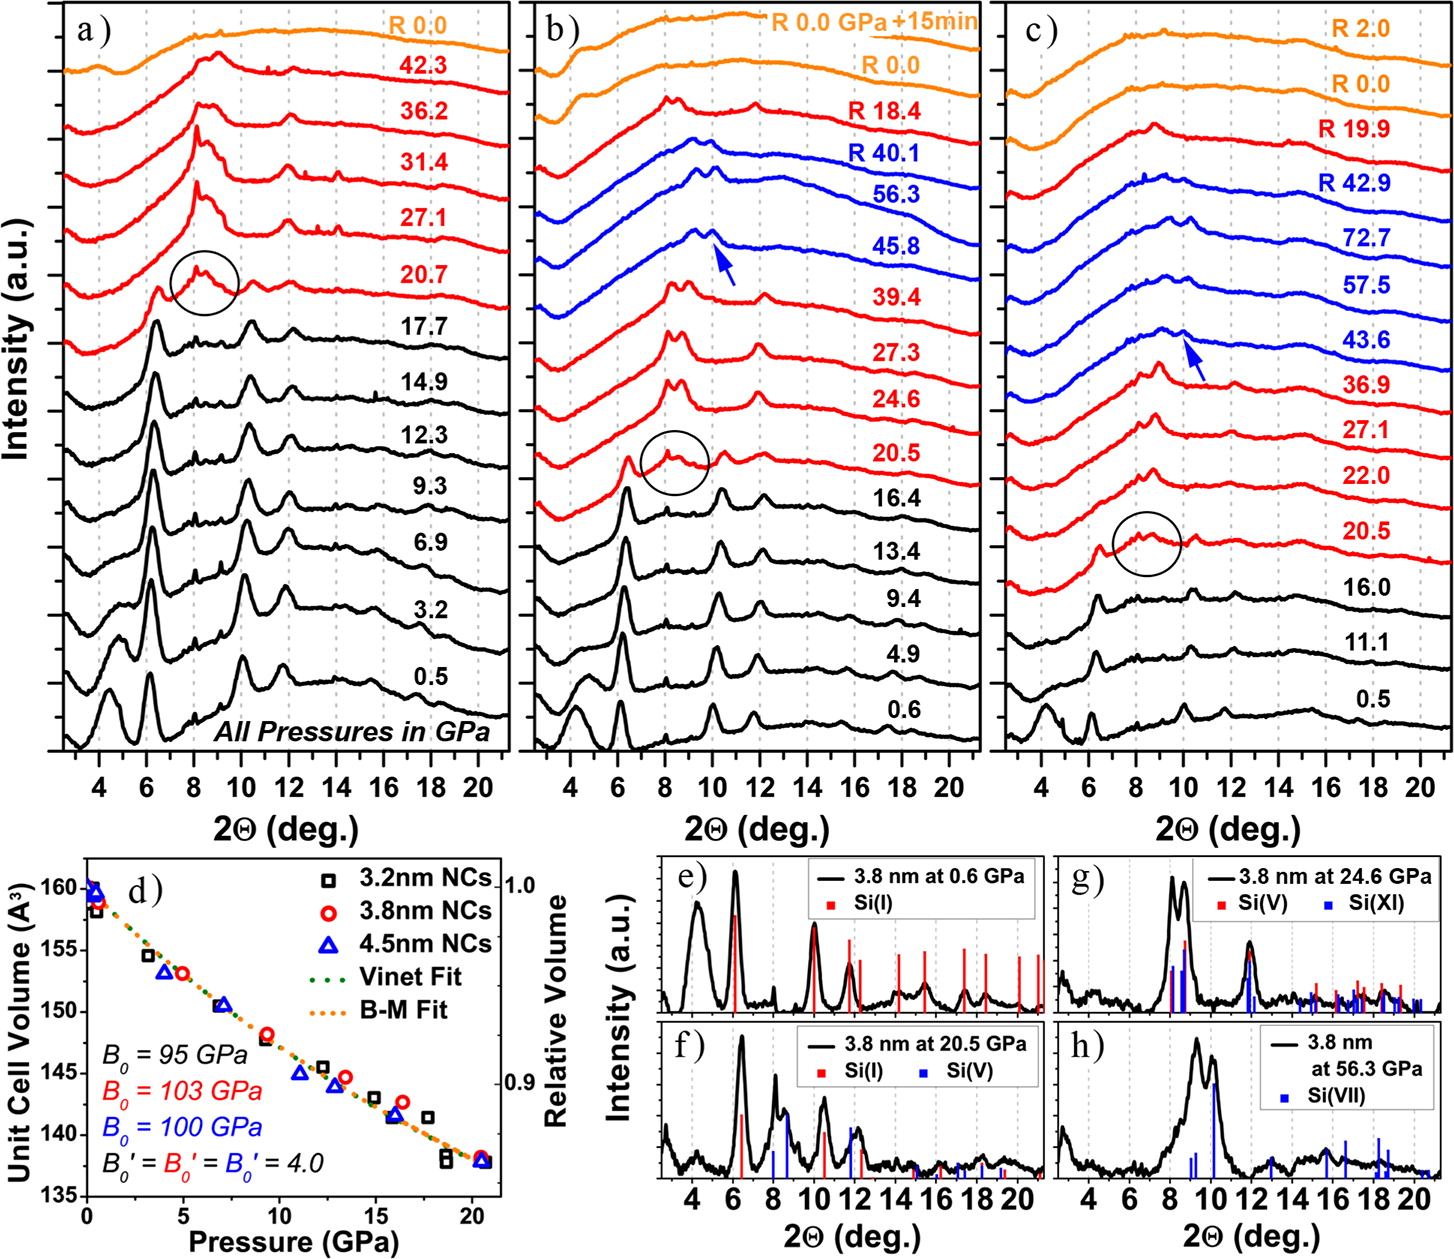
\includegraphics[width=\textwidth]{./chapter7/sipressure3.jpeg}
\caption[Pressure-dependent XRD patterns for Si NCs, phase analysis, and related XRD-derived structural data.]{Hydrostatic pressure-dependent XRD spectra for (a) 3.2 nm, (b) 3.8 nm, and (c) 4.5 nm diameter Si NCs. Graph colors indicate different identified crystalline phases of the Si NCs. Si(I) = black, Si(V) = red, Si(VII) = blue, and amorphous Si = orange. The peak circled in black at $\sim$20.5 GPa, corresponds to a new phase arising from the Si(I) phase. Arrows in (b,c) show sudden shifts of the peaks in Si(V), indicating transformation to a new phase. The “R” in the graph annotations indicates reversal of pressure (generally “downstroke”). (d) Unit cell volume data for Si(I) phase for all of the NCs sizes showed bulk moduli, B0, of $\sim$100 GPa with the derivative B0′ = 4.0, which matches bulk silicon. (e-h) Fits of the experimental data at the indicated pressures agree well with reported phases of bulk Si.}
\label{f:sipressure3}
\end{center}
\end{figure}

In these equations, $P_{300}$ is the pressure at 300 K, $B_0$ is the ambient pressure bulk modulus, $B_0'$ is the pressure derivative of the bulk modulus ($B_0 = dB_0/dP$), $V$ is the unit-cell volume, and $V_0$ is the ambient pressure unit cell volume. The bulk moduli for the 3.2 , 3.8 , and 4.5 nm NCs, respectively, were found to be 95, 103, and 100 GPa with a bulk modulus derivative of $B_0' = 4.0$ for all NC sizes.  This result shows that the bulk modulus of the NCs is (somewhat unusually) unchanged in comparison to bulk Si, which has a $B_0$ = 97.8 GPa \cite{hull1999properties}. Whereas NCs of binary semiconductors typically deviate from bulk-phase compressibility by at least 10 to 30\% \cite{PhysRevLett.101.217401,qadri1996pressure} likely owing to imperfect anion-cation stoichiometric ratios and surface charges at ligation sites, we suggest that Si NCs closely follow bulk behavior as neither of these issues are significant in this elemental material that experiences covalent Si-C surface termination. \par

In similarity to Tolbert's work on larger Si NCs coated with SiO$_2$, we observe elevation of the first phase transformation pressure when compared to the bulk material, which occurs at 11.7 GPa for the latter \cite{katzke2007structural}. The lowest pressure phase transformation in these alkane-terminated Si NCs occurs between 17 and 22 GPa and is accompanied by a notable increase of absorption, which was previously reported by Tolbert upon the semiconductor-to-metal phase transition. In all of the NC sizes, we observe the abrupt emergence of a new feature at 2$\theta$ $\approx$ 8.5$^{\circ}$ around $\sim$20.5-20.7 GPa (indicated with circles in Figure \ref{f:sipressure3}(a)-(c)). The emergent peak (Figure \ref{f:sipressure3}(f)) appears to correspond to a different phase that bears strong similarities with the phase observed by Tolbert et al. and is assigned to Si(V). The small size of our NCs results in substantial broadening of the diffraction peaks and does not permit ideal refinement of the structure. As such, we note that the new peak attributed to Si(V) also fits well to the Si(XI) structure (see Figure \ref{f:sipressure3}(g)). \par

Further compression of the Si NC samples reveals a new phase transformation between $\sim$40 and $\sim$44 GPa. While the separation of the first two peaks is similar to that of Si(V), the transformation is apparent owing to a sudden shift of the peaks and disappearance of one peak at $\sim$12$^{\circ}$. The new phase is a very close match to hcp Si(VII) when compared to the bulk-phase report by Olijynk \cite{olijnyk1984structural}. Furthermore, upon decompression we observe reversible recovery into the Si(V) structure at as low as 18.4 GPa, and finally, appearance of a-Si at ambient pressure. The a-Si was found to be stable, and XRD after 15 min or with pressure increases showed no reappearance of crystalline peaks.

\subsection{Germanium Nanocrystals}
Next, we present for the first time structural characterization of quantum-confined Ge NCs synthesized using two different methods. In particular, we study Ge NCs prepared using a previously described colloidal synthesis method \cite{lee2009colloidal} as well as Ge NCs prepared using a plasma synthesis method \cite{wheeler2013tunable} analogous to the one described in chapter 5. Both NC samples are covalently terminated with long-chain alkyl ligands (octadecane and dodecane, respectively). To study the pressure dependent structure of these Ge NCs, samples were loaded in diamond anvil cells according to the procedure described in chapter 5, with two exceptions. First, an X-ray energy of 30 keV, rather than 37 keV, was used. Secondly, rather than using ruby R1 fluorescence as a barometer, the $P$-$V$-$T$ equation of state for gold \cite{anderson1989anharmonicity} was used in conjunction with four diffraction lines (111, 200, 220, and 311) from a gold flake to determine the pressure. Both samples have a diameter of roughly 4 nm as determined by TEM analysis.

\begin{figure}
\begin{center}
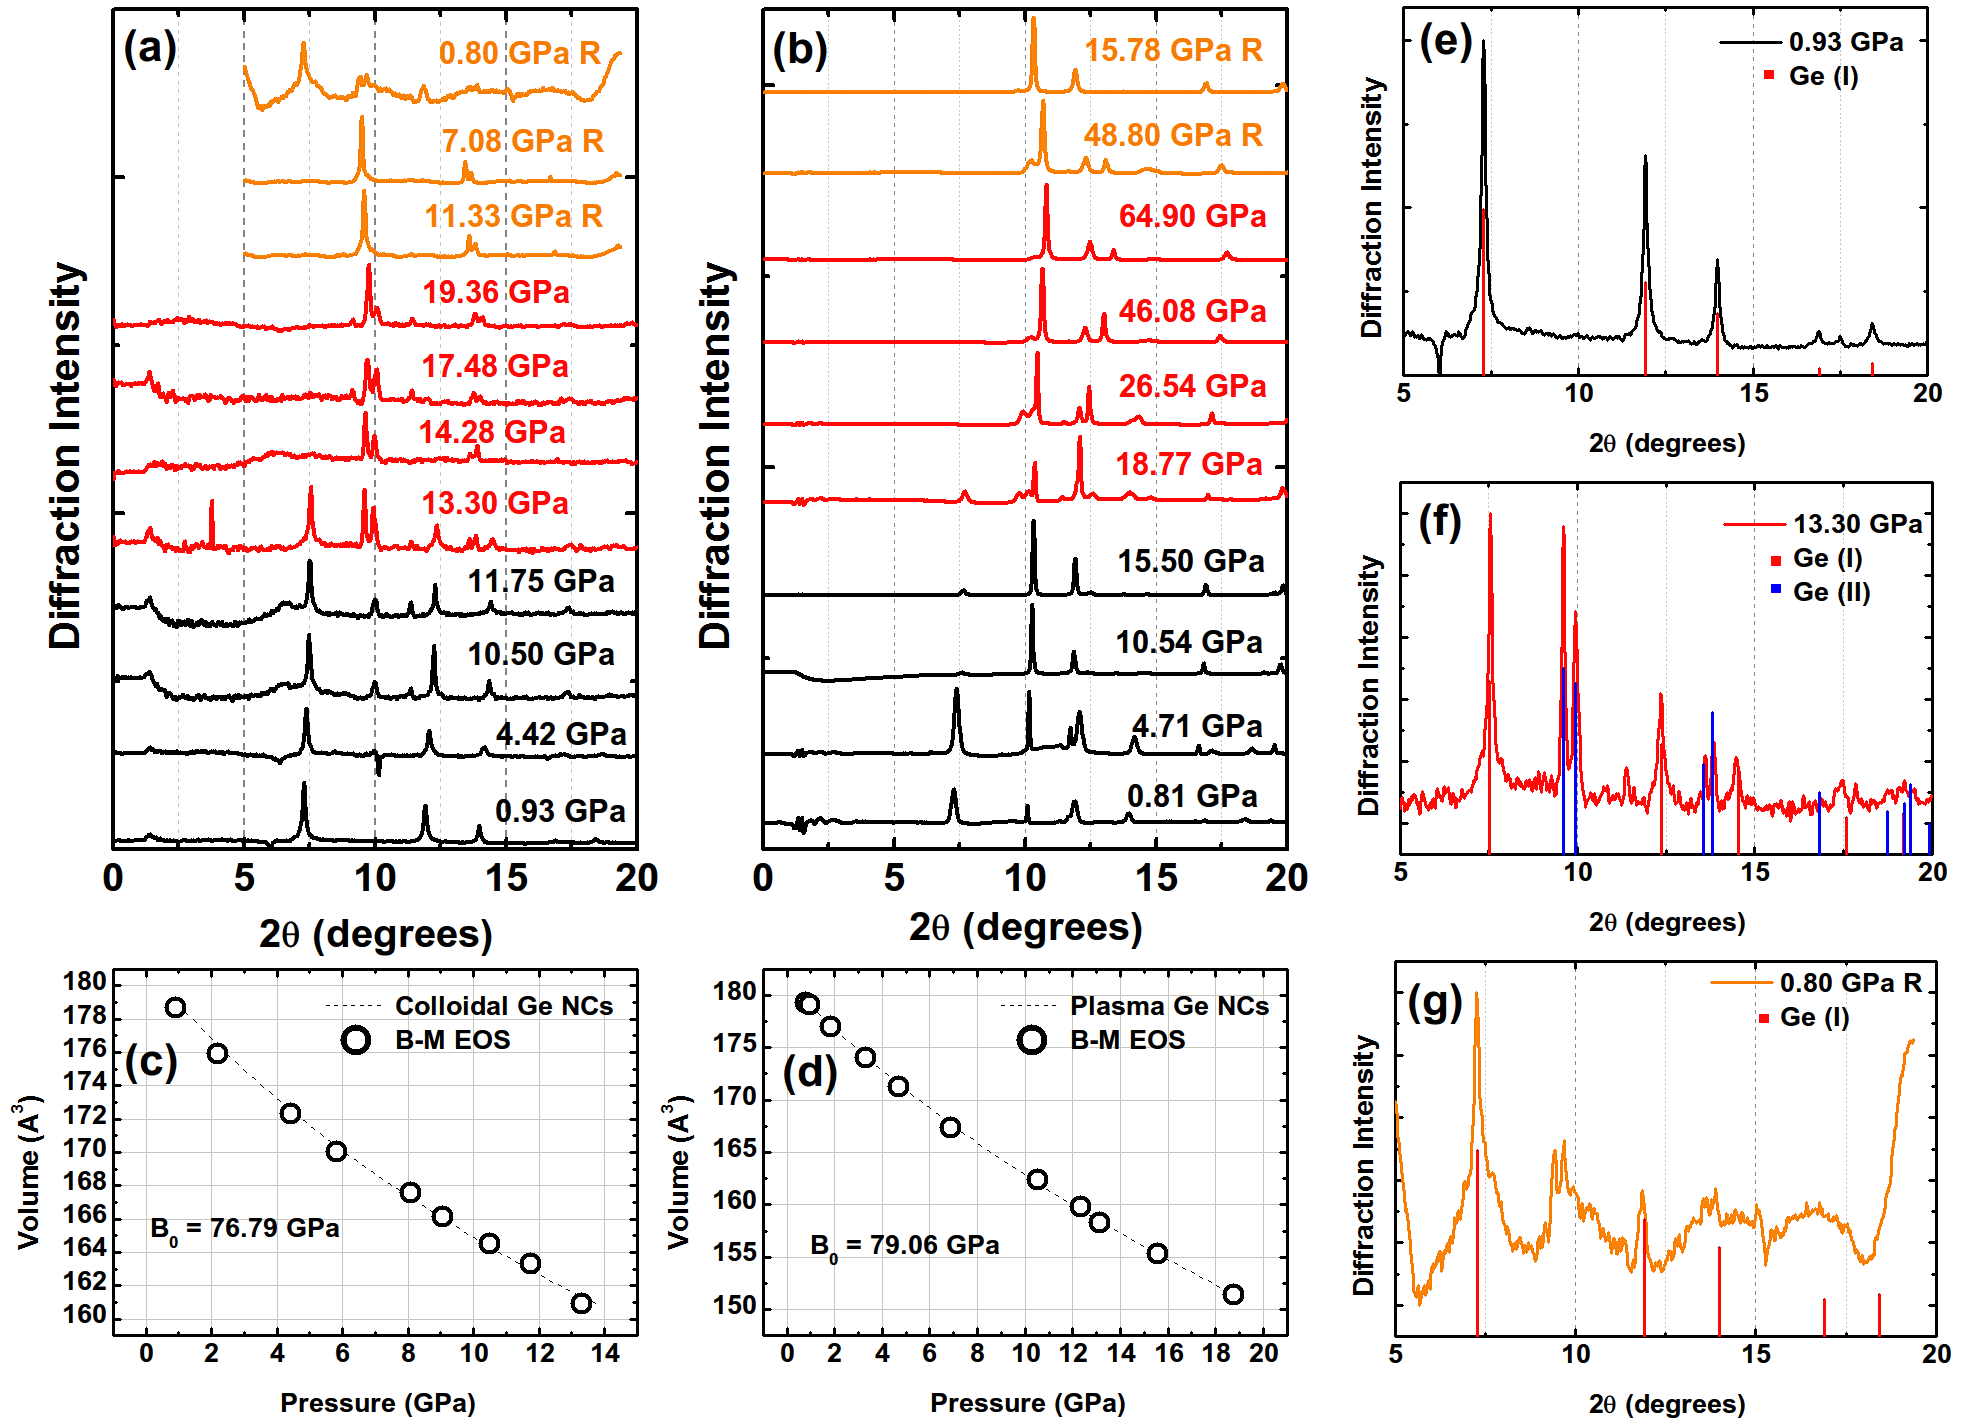
\includegraphics[width=\textwidth]{./chapter7/gepressure1.png}
\caption[Pressure-dependent XRD patterns for Ge NCs, phase analysis, and related XRD-derived structural data.]{(a) XRD patterns for 4 nm-diameter, colloidally synthesized Ge NCs at various indicated pressures.  Black curves indicate the presence of only the Ge(I) phase.  Red curves indicate the Ge(II) phase.  Orange curves indicate diffraction patterns acquired on pressurization downstrokes ("R") subsequent to pressurization to 19.36 GPa.  (b) XRD patterns for 4 nm-diameter, plasma synthesized Ge NCs at various applied pressures (indicated).  (c) XRD-derived unit cell volume as a function of pressure for colloidally synthesized NCs, along with a fit to the Burch-Murnaghan (B-M) equation of state and the resulting bulk modulus ($B_0$). (d) Same as (c), but for plasma-synthesized NCs. (e)-(g) Indicate XRD pattern for 4 nm-diameter, colloidally synthesized Ge NCs at (e) 0.93 GPa, with red vertical lines indicating the diffraction angles for the Ge(I) phase.  (f) 13.30 GPa, with red vertical lines indicating the diffraction angles for the Ge(I) phase and blue vertical lines indicating the diffraction angles for the Ge (II) phase.  (g) 0.80 GPa following pressurization to 19.36 GPa and subsequent depressurization to 0.80 GPa in roughly 5 GPa steps.  Red lines indicate diffraction angles for the Ge (I) phase.}
\label{f:gepressure1}
\end{center}
\end{figure}

Figure \ref{f:gepressure1} presents the experimental results of this XRD study of Ge NCs. Fig. \ref{f:gepressure1}(a) shows XRD patterns for the colloidally prepared Ge NCs referenced above, while Fig. \ref{f:gepressure1}(b) shows XRD patterns for the plasma-synthesized sample.  The colloidally prepared sample exhibits the Ge(I) (cubic, diamond) structure at ambient pressures. Diffraction peaks associated with the metallic Ge(II) ($\beta$-Sn) phase become apparent at $\sim$13 GPa, suggesting a phase transition which is elevated relative to bulk Ge \cite{PhysRevB.34.362}. Upon reversal of the pressure, the Ge NCs exhibit structural hysteresis, with Ge(II) peaks still present at a pressure of $\sim$7 GPa. Eventually, at 0.8 GPa, the Ge(I) phase is recovered. The plasma synthesized sample (Fig. \ref{f:gepressure1}(b)) exhibits similar behavior, but with a slightly elevated Ge(I) $\rightarrow$ Ge(II) phase transition pressure of 16.77 GPa. While experimental difficulties limited the maximum pressure of the colloidal Ge NC studies to 20 GPa, the plasma-synthesized NCs were pressurized to 70 GPa.  Upon depressurization, these samples also exhibit slight recovery of the Ge(I) phase. This is in contrast to Si, which exhibits complete and irreversible amorphization of the sample upon depressurization following a transition to the $\beta$-Sn phase. Figures \ref{f:gepressure1}(e), (f), (g) display a phase analysis of the XRD data, with vertical lines indicating the known diffraction peak positions for the Ge phases described here. \par
Figures \ref{f:gepressure1}(c) and (d) display unit cell volume for both Ge samples as a function of applied pressure, determined in the same fashion as for Si NCs and described above. Again, we fit these data to the third order Birch Murnaghan equation of state (Eq. \ref{eq:sipressure1}). The data are fit by Eq. \ref{eq:sipressure1} extremely well and yield bulk moduli of 76.79 GPa for the colloidal sample and 79.06 GPa for the plasma-synthesized sample. Both of these values are comparable to the 78 GPa bulk modulus reported for bulk Ge. A similar agreement between nanoscale and bulk phases is noted for Si above, but this agreement is in stark contrast to binary NC compositions. 

\section{Molecular Dynamics Simulations of Nanocrystal Pressurization}

To further explore the interesting structural behavior observed experimentally and presented above, we performed MD simulations of Si and Ge nanoparticles experiencing hydrostatic pressure applied by a pressure-transmitting medium. Our pressurization routine is the same used to derive the pressurized NC structures presented in chapter 5, which we elaborate on here. A faceted nanoparticle is first generated using experimentally known surface energies along with the Wulff construction. A box containing roughly 200,000 argon atoms (depending on NC size) is also created, and the Si NC placed in the center. Following this, any argon atoms having positions within 2\r{A} of a Si NC atom are deleted. Si-Si, Si-H, Ge-Ge, and Ge-H interactions are modeled according to the Tersoff potential \cite{PhysRevB.37.6991}. Interactions between the NC atoms (group-IV elements and H) and the fluid are modeled by a Lennard-Jones potential. Fluid-fluid interactions are modeled by a purely repulsive Lennard-Jones potential (i.e. cutoff set to $2\sigma^{1/6}$) to avoid freezing of the pressure-transmitting medium at high pressure. A timestep of 0.1 fs used to allow for accurate simulation of Si-H and Ge-H vibrations. After the initial geometry is created, the system is simulated for 2 ps in the NVE ensemble to allow fluid atoms to fill the space left by the deletion procedure described above. After that step, the system is simulated in the NPT ensemble (starting at 0 GPa) for a 15 ps equilibration run; this was determined to be sufficient to stabilize the pressure and temperature in the system. Following equilibration, a 5 ps production run was carried out. After production, the pressure is increased in steps of 0.25 GPa and the procedure repeated.

\subsection{The Impact of Surface Termination}

While utilizing MD simulations to explore the wurtzite-to-rocksalt phase transformation in CdSe nanocrystals, Gr{\"u}nwald and co-workers note the importance of including surface passivation due to its effect on NC surface energies \cite{grunwald2006mechanisms}. A number of studies have noted that pressure-induced phase transitions in CdSe begin with nucleation events on the NC surface \cite{grunwald2006mechanisms, grünwald2009nucleation, grunwald2009transition, grünwald2012metastability}. Because binary NCs can (and in practice often do) exhibit ion-rich surfaces, it is possible that that the elemental composition (rendering non-stoichiometric surfaces impossible) of group-IV NCs is responsible for the compressibility identical to that of the bulk phase. While the exact role played by the surface is a multifaceted issue, because surface ligands likely affect interactions with the solvent as well as the surface energies, we do note here that surface termination clearly affects NC response to applied hydrostatic pressure.

\begin{figure}
\begin{center}
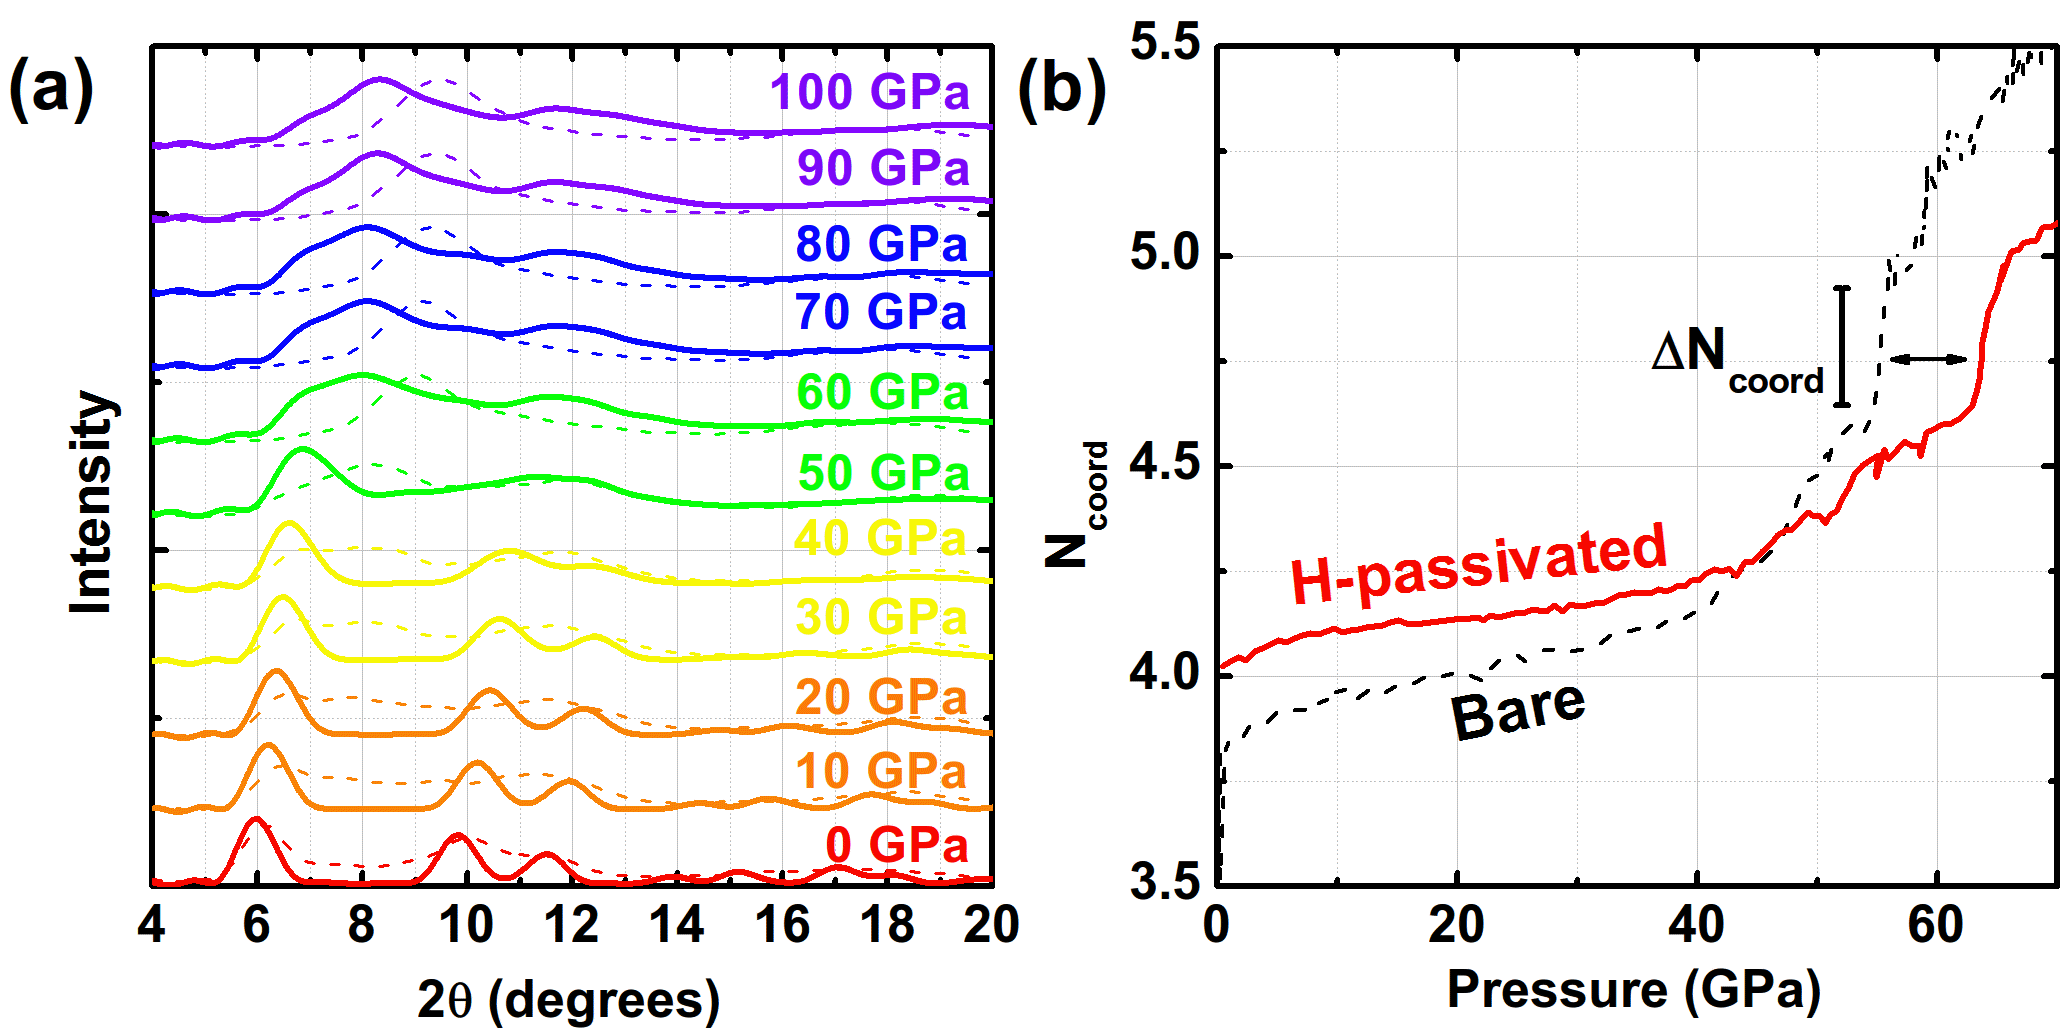
\includegraphics[width=\textwidth]{./chapter7/md1.png}
\caption[Comparison of simulated XRD and coordination number for bare and H-passivated Si NCs.]{(a) Simulated XRD patterns for a 2.4 nm-diameter Si NC at pressures spanning 0-100 GPa. Pressures are color-coded and indicated on the figure. Solid lines represent an H-passivated Si NC, while dashed lines represent a bare Si NC. (b) Average number of nearest numbers for each atom as a function of applied pressure for a bare (black, dashed lines) and passivated (red, solid lines) Si NC. $\Delta$N$_{\mathrm{coord}}$ indicates a discontinuity in the coordination number likely associated with a phase transition.}
\label{f:md1}
\end{center}
\end{figure}

Figure \ref{f:md1}(a) displays the simulated XRD diffraction pattern for a bare and H-terminated 2.4 nm-diameter Si NCs spanning pressures from 0-100 GPa. We calculate X-ray diffraction patterns by solving the Debye scattering equation:
\begin{equation}\label{eq:debye}
I(Q) = \sum_i\sum_j f_i f_j \frac{\sin{Q|\vec{r}_i - \vec{r}_j|}}{Q|\vec{r}_i - \vec{r}_j|}
\end{equation}
In Equation \ref{eq:debye}, $|\vec{r}_i - \vec{r}_j|$ is the distance between atoms $i$ and $j$, $f_i$ is the atomic scattering factor of atom $i$; this is an element-specific quantity which is wavelength-dependent and known in general, and $Q$ is scattering vector, related to the experimental X-ray wavelength $\lambda$ via $Q = |\vec{Q}| = 4\pi\sin{\theta/\lambda}$. In calculating the XRD patterns presented here we utilized the experimental X-ray energies (30 keV for Ge and 37 keV for Si). While the behavior exhibited by each nanocrystal is qualitatively similar, the structural evolution of the H-terminated NC seems to lag behind the bare NC. This is reflected in an analysis of the average coordination number presented by Si atoms in each simulation, shown in Fig. \ref{f:md1}(b). In particular, a phase transition, as evidenced by a discontinuity in the average coordination number seems to occur at $\sim$50 GPa for the bare NC, while a similar discontinuity is seen at $\sim$60 GPa for the H-passivated NC. While both of these pressures are considerably higher than the phase transition pressures observed experimentally, this is likely to the utilization of the Tersoff potential, which knowingly overestimates the absolute phase transition pressure but correctly captures trends and mechanisms in the bulk phase \cite{durandurdu2008diamond, PhysRevB.50.14952}. For the work presented in this chapter, we have studied H-passivated Si and Ge NCs; while these species are not an exact mimic of the alkyl termination experienced by the particles studied experimentally, the H-passivation scheme still presents a covalent surface bond while remaining computationally tractable.

\subsection{Comparison of Experimental and Simulated Structural Changes}

\begin{figure}
\begin{center}
\includegraphics[width=\textwidth]{./chapter7/md2.png}
\caption[Comparison of simulated and experimental XRD patterns for passivated Si NCs.]{(a) Comparison of experimentally-observed (black) and MD derived (red) XRD patterns for Si NCs at ambient pressure. (b) Comparison of experimentally-observed (black) and MD derived (red) XRD patterns for Si NCs at pressures sufficient to induce a phase transition (140 GPa for MD, 42.3 GPa for experiment).}
\label{f:md2}
\end{center}
\end{figure}

Excepting the higher absolute pressure values needed to produce structural changes (likely related to the usage of a Tersoff interaction potential; see above), the computational pressurization scheme utilized here produces structures which agree well with those observed experimentally.  Figure \ref{f:md2} compares simulated and experimentally-observed XRD patterns for the low- and high-pressure phases of Si NCs. Fig. \ref{f:md2}(a) displays excellent agreement for the ambient-pressure structures, while \ref{f:md2}(b) also displays good agreement for the high-pressure phase. Note that while the pressure is much higher (140 GPa in the MD simulation compares reasonably well to an experimental pressure of 42.3 GPa), the peaks near 8$^{\circ}$ and 12.5$^{\circ}$ are associated with the $\beta$-Sn phase and are produced in both patterns. \par
We also note good agreement for Ge NCs. Figure \ref{f:md3}(a) displays a range of simulated XRD patterns for a 4 nm-diameter, H-passivated Ge nanocrystal at pressures spanning 0-100 GPa. The structure seems to undergo a large change between 50 and 60 GPa. Fig. \ref{f:md3}(b) compares the low- and high-pressure phases observed in our simulations to those observed experimentally (Fig. \ref{f:gepressure1}). Both phases show agreement, again with an elevated pressure (60 GPa) required to produce agreement with the experimental high-pressure phase (19 GPa). The peaks at 10$^{\circ}$ and 14$^{\circ}$ are characteristic of the $\beta$-Sn phase of Ge \cite{PhysRevB.34.362} and are present in both the simulated and experimental patterns. The agreement between experimentally-observed and simulation-derived XRD patterns suggests that the method of pressurization utilzied here is a suitable means of generating atomistic configurations of pressurized NCs.

\begin{figure}
\begin{center}
\includegraphics[width=\textwidth]{./chapter7/md3.png}
\caption[Simulated XRD patterns at a range of pressures and comparison of simulated and experimental XRD patterns for passivated Ge NCs.]{(a) Simulated XRD patterns for a 4 nm-diameter, H-passivated Ge NC at pressures spanning 0-100 GPa. Pressures are color-coded and indicated on the figure. (b) Top: Comparison of experimentally-observed (black) and MD derived (red) XRD patterns for Ge NCs at ambient pressure. Bottom: Comparison of experimentally-observed (black) and MD derived (red) XRD patterns for Ge NCs at pressures sufficient to induce a phase transition (60 GPa for MD, 19 GPa for experiment).}
\label{f:md3}
\end{center}
\end{figure}

\subsection{Analysis of Phase Transitions}

To obtain a quantitative measure of the local coordination environment of a given atom, we utilize an ordering parameter $q$,\cite{PhysRevB.28.784} which has been used previously to quantify nucleation events in supercooled liquid Si \cite{li2009nucleation}. We first compute the term $\bar{q}$, which is shown in Equation \ref{eq:md1}:
\begin{equation}\label{eq:md1}
\bar{q}_{lm}(i) = \frac{1}{N_b\left(i\right)}\sum_{j=1}^{N_b\left(i\right)} Y_{lm}\left(\theta\left(\vec{r}_{ij}\right), \phi\left(\vec{r}_{ij}\right)\right)
\end{equation}
In Eq. \ref{eq:md1}, $N_b(i)$ is the number of bonds for particle $i$, while $\theta$ and $\phi$ denote the azimuthal and polar angles of orientation for bond $\vec{r}_{ij}$. $Y_{lm}$ denote the spherical harmonics. From $\bar{q}_{lm}$, we may construct a $2l+1$ dimensional vector $\vec{q} = \left[\bar{q}_{l,-l}, \bar{q}_{l,-l+1}, ..., \bar{q}_{l, l-1}, \bar{q}_{l,l}\right]$ for each atom $i$ and compute:
\begin{equation}\label{eq:md2}
q_l = \frac{1}{N_b\left(i\right)}\sum_{j=1}^{N_b\left(i\right)}\frac{\vec{q}_l\left(i\right)\cdot\vec{q}_l\left(j\right)}{|\vec{q}_l\left(i\right)||\vec{q}_l\left(j\right)|}
\end{equation}

\begin{figure}
\begin{center}
\includegraphics[width=\textwidth]{./chapter7/md4.png}
\caption[Analysis of NC coordination environment using an ordering parameter and pressure-dependent crystal phase populations during MD simulations of pressurization.]{(a) and (b) display the distribution of local ordering parameter $q_4$ (Eq. \ref{eq:md2}) for Si and Ge NCs, respectively. In both (a) and (b), red bars represent the ambient-pressure histogram and blue bars represent the high-pressure histogram, with the pressures corresponding to each phase labeled on the figure. Both (a) and (b) also display a dashed line indicated the critical $q_4$ value, $q_c$, used to distinguish between phases. (c) and (d) display the number of atoms having either a diamond (red) or $\beta$-Sn environment (blue) as determined by the cutoff parameter $q_c$ for Si and Ge NCs, respectively.}
\label{f:md4}
\end{center}
\end{figure}

Figures \ref{f:md4}(a) and (b) show the distribution of of these local parameters using the fourth order spherical harmonics, which were found to produce the best discrimination between diamond and $\beta$-Sn phases. In order to quantify the local environment of atom $i$, a critical value $q_c$ is chosen such that atoms having $q_i < q_c$ are classified as one phase, while atoms having $q_i > q_c$ are classified as the other. For Si, atoms having $q_i < q_c$ are diamond phase, while the reverse is true for Ge (see Fig. \ref{f:md4}(a) and (b)). Using this criterion, the number of "diamond"-coordinated and the number of "$\beta$-Sn"-coordinated atoms was calculated along the range of pressures simulated. This is shown for a 2.4-nm diameter Si NC and a 4 nm-diameter Ge NC in Figure \ref{f:md4}(c) and (d) respectively. The diamond and $\beta$-Sn populations, for both NCs, show a rapid inflection and inversion around the the pressures indicated as phase transitions by XRD and nearest neighbor counting (see Figures \ref{f:md1} and \ref{f:md3}). This suggests that the choice of $q_c$ is suitable for analyzing the phase transition.\par

\begin{figure}
\begin{center}
\includegraphics[width=\textwidth]{./chapter7/md5.pdf}
\caption[Snapshots from MD simulations of NC pressurization color-coded according to ordering parameter analysis.]{Snapshots of NCs labeled according to composition and pressure. Each snapshot has atoms color coded according to coordination environment: Red for diamond, and blue for $\beta$-Sn, determined by the paramter $q_c$ as described in the main text. While pressure-transmitting fluid atoms and passivating H atoms are present in the simulation, they are not rendered in these snapshots.}
\label{f:md5}
\end{center}
\end{figure}

Figure \ref{f:md5} displays snapshots from the MD simulation trajectory for a Si and Ge NC. Atoms in Fig. \ref{f:md5} are colored according to their phase, determined as described above. Continuing the color scheme used in Fig. \ref{f:md4}, diamond atoms are colored red, while $\beta$-Sn atoms are colored blue. Both the Si and Ge particles display a noticeable but small contraction of the NC volume and a near-complete conversion to the $\beta$-Sn phase at high pressures. While both structures, and in particular the Ge NC, perhaps show a slight bias toward a surface-inward mechanism, it is not readily apparent from visual inspection of the trajectories alone what the spatial distribution of diamond- and $\beta$-Sn-coordinated atoms is along the trajectory.\par
The radial and pressure-dependent $q$ value for each Si (Ge) atom is plotted in Figure \ref{f:md6}(a)((b)). The Si NC shows little bias toward the surface.  While some atoms just beneath the surface quickly shift their coordination environment, the vast majority of atoms cross over the transition together, evident by the nearly-vertical front of $\beta$-Sn-coordinated atoms emerging at $P \approx 50$ GPa. The Ge NC, however, shows a significant fraction of surface atoms experiencing a $\beta$-Sn-like coordination environment at modest presssures prior to the major phase transition at $P \approx 60$ GPa, where a similar onset of $\beta$-Sn coordination appears. 

\begin{figure}
\begin{center}
\includegraphics[width=\textwidth]{./chapter7/md6.png}
\caption[Dependence of atomic coordination on radius and pressure during MD simulations of NC pressurization.]{(a) and (b) display the coordination environment (either diamond - red, or $\beta$-Sn - blue, determined by $q_c$ as described in the main text) as a function of pressure and NC radius for Si and Ge NCs, respectively. The sharp onset of $\beta$-Sn atoms at a particular pressure is indicative that a majority of NC atoms experience the phase transition together.}
\label{f:md6}
\end{center}
\end{figure}

\subsection{Results and Discussion}
It is worth noting that the results presented here are a preliminary study and are part of a larger work in progress. The size-dependence of the results will be especially important in determining the actual phase transition mechanism. While the Ge NC seems to exhibit the transition of surface atoms prior to core atoms, the Ge NC studied in this chapter is larger (4 nm-diameter) than the Si NC (2.4 nm-diameter). It is possible that 4 nm-diameter Si NCs may show a similar bias. Nevertheless, even the 4 nm-diameter Ge NC exhibits a simultaneous transition of a majority of atoms in the structure, and certainly to a greater extent than was observed in MD simulations of pressure-induced structural changes in CdSe NCs \cite{grünwald2012metastability}. This may suggest that the surface plays less of a role in initiating phase transitions in group-IV NCs than is the case for II-VI ionic NCs, and may explain the bulk-like compressibility of group-IV NCs noted here, as only a negligible fraction of atoms in bulk materials exist on surfaces. \par
Further work will be required to fully explore the origin of bulk-like compressibility in group-IV NCs and fully understand the mechanism of pressure-induced phase transitions in these materials. Firstly, while the Tersoff potential is known to overestimate the diamond $\rightarrow \beta$-Sn phase transition, there are also kinetic and statistical factors which are more appropriately treated by more advanced sampling methods. Because solid-solid transformations typically involve high kinetic barriers, phase transitions are statistically rare events under hydrostatic compression near the phase transition pressure \cite{grunwald2009transition, wittenberg2014real}. This typically requires observation timescales or size scales out of range of atomistic simulations. Instead, as we have done here, the usual solution is to simulate elevated pressures such that transformations readily occur on accessible timescales. Thus, it is possible that the mechansims observed here differ from those observed experimentally. A more rigorous analysis will necessarily utilize transition path sampling or forward-flux sampling algorithms capable of efficiently simulating statistically rare events \cite{grunwald2009transition, li2009nucleation}.

\section{Conclusions}
In this chapter we presented a characterization of pressure-induced structural changes in Si and Ge NCs. Colloidal dispersions of Si or Ge NCs were loaded into diamond anvil cells, pressurized, and examined using synchrotron-derived XRD. As has been observed for other NCs, Si and Ge nanocrystals exhibit elevated phase transition pressures relative to the bulk phase. In constrast to other NCs, however, both Si and Ge NCs exhibit a compressibility matching the bulk phase. To explore the origin of this behavior, we also carried out and presented here MD simulations of NC pressurization \emph{via} a pressure-transmitting fluid in a rough mimic of the actual diamond anvil cell experiment. Firstly, we noted good agreement between experimentally-observed and MD-derived XRD patterns, indicating the that use of a pressure-transmitting fluid is a suitable method for generating NC structures that resemble those generated during diamond anvil cell pressurization.\par
We also demonstrated that an ordering parameter based on spherical harmonics is capable of discriminating between low- (diamond) and high-pressure ($\beta$-Sn) phases in group-IV NCs. Using this ordering parameter, we found that a majority of NC atoms transition from $q < q_c$ to $q > q_c$ (that is, from diamond-like coordination to $\beta$-Sn-like coordination) collectively. This is somewhat in contrast to prior studies on CdSe NCs which suggest surface-led nucleation of the high-pressure phase. While we emphasize that more advanced MD trajectory sampling algorithms are necessary to confirm the phase transition mechanism explored here, our preliminary results suggest that group-IV NCs experience phase transitions in a more collective, rather than surface-dominated fashion. This may explain the bulklike compressibility of these NCs relative to binary NC compositions.

\chapter{Concluding Remarks}

\section{Dissertation Summary}

This dissertation explores two major themes in nanoscience: Heat generation/transport and light emission from nanostructured Si. Chapters 2, 3, and 4 address the former issue. In chapter 2, we examine the early stages of heat generation - that is, the conversion of carrier energy to lattice heat. We utilize a recently developed spectroscopic method, femtosecond stimulated Raman spectroscopy (FSRS), which is unique in its ability to resolve low-frequency vibrational populations with subpicosecond time resolution. We are able to directly measure, for the first time, carrier-cooling by phonon emission in CdSe nanocrystals (NCs). We find that electrons cool primarily \emph{via} resonant, Auger-like energy transfer to holes, which cool by emitting phonons. These results demonstrate the utility of FSRS in quantitatively measuring the dissipation of excitonic energy into other degrees of freedom and confirm as-yet unproven theories regarding electron-to-hole energy transfer. In chapter 2 we also present theoretical modeling which provides a mechanism for the slowdown of electron-phonon thermalization in small plasmonic nanoparticles upon thiol-passivation. Considering the growing utility of plasmonic nanostructures in generating hot electrons for e.g. catalysis, these results should provide guidance to researchers hoping to manipulate hot electron lifetimes. \par
Chapter 3 addresses issues related to nanoscale thermal transport. First, we present our discovery of a dynamic optical signature of acoustic phonon transport out of semiconductor NCs. By measuring the size-dependent rate of this signature we are able to demonstrate that heat transport of matrix-embedded NCs occurs on a 10-100 ps time scale in a diffusion-limited fashion. We also utilize MD simulations to demonstrate that in addition to surface ligands mediating interfacial thermal conductance, the structure of the underlying semiconductor surface plays an important role by determining the grafting density of these ligands. We expand on this knowledge in chapter 4, which focuses on making structural modifications to NCs to manipulate thermal processes. Here, we utilize the aforementioned optical signature of thermal outflow to demonstrate that the growth of a wide-bandgap semiconductor shell permits independent tuning of NC optical and thermal properties. Furthermore, we present theoretical results which suggest that passivation of NC surfaces with small, inorganic ligands or covalently bound species may provide similar thermal benefits but without confining charge carriers to the NC core. \par
Chapters 5 and 6 focus on group-IV NCs. In chapter 5, we examine long-lived PL (PL) from Si NCs. Using pressure-dependent PL spectroscopy along with combined quantum-classical modeling, we definitively assign red PL to band-edge emission from NC core states, which exhibits indirect-gap character despite substantial quantum confinement. For the first time, we also spectrally and temporally resolve high-energy PL and associate it with a persistent amorphous surface layer, a conclusion we support using TEM, Raman, and MD simulations. \par
In chapter 6, we explore interesting structural properties of Si and Ge NCs. We report XRD characterizations of these NCs at pressures ranging from 0-100 GPa. As has been observed in other NCs, both Si and Ge exhibit elevated phase transition pressures relative to the bulk phase. Interestingly, in stark constrast to binary semiconductor NC compositions, we note compressibility values matching the bulk phase for both Si and Ge. We explore the possible origins of this behavior using MD simulations, with a focus on the role played by the surface.

\section{Future Directions}

\subsection{Heat Generation/Transport}
Chapters 2-4 have provided a much clearer picture of the processes and parameters governing heat generation and transport in semiconductor NCs. They also present results which demonstrate that structural modifications affect these processes in a controllable way. A promising next step for work in this area is to explore the role of dimensionality. For example, do phonon population dynamics differ significantly in nanorods (1D) or nanoplates (2D)? Samples exhibiting multiple observable vibrational modes are also ripe for study: By correlating population transfer between modes having a known spatial separation, one could answer open questions regarding the physics of heat transport at nanometer length scales. Another avenue regarding dimensionality is suggested by the simulations in chapter 3 - might it be possible to engineer directional heat flow by synthesizing structures which preferentially expose high-thermal-conductance surfaces? Finally, thermostatting and barostatting algorithms have recently been developed which enable the application of non-equilibrium MD simulations to non-periodic systems, such as an isolated nanoparticle in a solvent droplet. We are currently applying these methods to colloidal NC structures to obtain a fully atomistic, theoretical picture of heat transport in such systems.

\subsection{Light Generation}
While chapter 5 thoroughly explores the origin of PL in plasma-synthesized Si NCs, it will be important to examine whether other synthetic routes yield particles presenting an (emissive) amorphous surface layer. We are also currently investigating the origin of PL in Ge NCs. While Si NC PL was shown to be dominated by an indirect-gap transition, one might expect quantum confinement to more strongly mix the direct- and indirect-gap transitions in Ge, which are far more energetically proximal than in Si. \par
Finally, the interesting pressure-dependent structural behavior of group-IV NCs prompts several open questions. Why does compressibility of group-IV NCs match the bulk phase while binary NC compositions differ significantly from bulk in this regard? What is the exact role of the surface in mediating the structural response of NCs to applied pressure? Answering these questions may enable surface chemistry-based approaches to tuning the mechanical properties of nanostructures. While we have made some progress toward answering these questions using MD simulations and present this work in chapter 6, there are many avenues open for further exploration. In particular, efforts are underway to utilize transition path sampling algorithms with the aim of more realistically simulating NC phase transitions. 

% Alternatively, you may write the chapters in separate
% files, say chap1.tex, chap2.tex, etc., and include them 
% with commands:

%\chapter{Introduction}	% The first Chapter.
Quantum-confined semiconductor nanocrystals (NCs) are crystalline clusters of atoms having a semiconductor composition with diameters smaller than the spatial extent of the electron and/or hole wavefunction in the corresponding bulk material. In this case, that particular carrier is said to be experiencing quantum confinement. While such materials are also commonly referred to as quantum dots, we refer to this material class (colloidal, quantum confined semiconductor nanocrystals) as NCs to distinguish them from the various other types of quantum dots common in the literature, such as epitaxial self-assembled quantum dots or gate-defined quantum dots. In this thesis, we focus on cluster sizes and materials for which \emph{both} carriers are strongly confined. In general, NCs exhibit size-dependent, broadly tunable absorption and emission spectra, near-unity quantum yields, and are amenable to low-cost, easily scalable solution-phase processing. Furthermore, they exhibit emergent physical processes such as hot electron transfer and carrier multiplication. As a result, they have been suggested as a means to improve a wide variety of energy-relevant technologies including LEDs, lasers, solar cells, transistors, and thermoelectric power converters. Since their initial synthesis in 1985, the optical and electronic properties of NCs have received a great deal of attention, and a great deal is now understood regarding the electronic structure of this fascinating material class. We review some important aspects of NC electronic structure and optical properties here. As the work presented in this thesis is concerned with nanoscale energy generation and dissipation, we also review the basics of phonon-assisted carrier cooling and thermal transport.

\section{Quantum Confinement and Electronic Structure}
\subsection{Particle-in-a-Sphere}
The remarkable effects of quantum confinement are most easily understood by considering the NC as a particle-in-a-sphere \cite{efros1982interband, brus1986electronic}, analogous to the particle-in-a-box problem familiar from quantum mechanics. We will begin by applying spherical boundary conditions to a bulk semiconductor wavefunction. The spherical boundary conditions applied here take the form of an infinite spherical potential of radius $a$, $V(\vec{r})$, such that:
\begin{equation}\label{eq:pis1}
V(\vec{r}) = \left\{
	\begin{array}{ll}
		0 & \mbox{if } \vec{r} < a \\
		\infty & \mbox{if } \vec{r} > a
	\end{array}
\right.
\end{equation}

As a starting point, we utilize Bloch's theorem, which states that in a perfectly crystalline and periodic material, we may write the carrier wavefunction as the product of a wavelike portion and a cell-periodic portion, as shown below:
\begin{equation}\label{eq:pis2}
\Psi_{n\vec{k}}(\vec{r}) = u_{n\vec{k}}e^{i\vec{k}\cdot\vec{r}}
\end{equation}
In Equation \ref{eq:pis2}, the function $u_{n\vec{k}}$ is a function with the periodicity of the crystal lattice, with the wavefunctions being labeled by band index $n$ and wavevector $\vec{k}$. Eigenvalues of the Schr{\"o}dinger equation for Eq. \ref{eq:pis2} yield an energy spectrum of the form:
\begin{equation}\label{eq:pis3}
E_{n}\left(\vec{k}\right) = \frac{\hbar^2\vec{k}_n^2}{2m_{\mathrm{eff}}}
\end{equation}
In Eq. \ref{eq:pis3} we have utilized the so-called effective mass approximation, in which semiconductor carriers behave as free particles but with an altered ("effective") mass compensating for the complex potential experienced by the carriers due to the host lattice. In the effective mass approximation, the valence and conduction bands are assumed to have parabolic forms, evident in the $\vec{k}^2$ dependence of the energy levels (Eq. \ref{eq:pis3}) and demonstrated graphically in Figure \ref{f:pis1}. \par

\begin{figure}
\begin{center}
\includegraphics[width=0.5\textwidth]{./Chapter1/parabolic.pdf}
\caption[Two-band model for a direct gap semiconductor in the parabolic band approximation.]{Two-band model for a direct gap semiconductor in the parabolic band approximation. The true band structure is shown in solid lines, while the parabolic bands, centered at $\vec{k} = 0$ utilized in the effective mass approximation are shown in dashed lines.}
\label{f:pis1}
\end{center}
\end{figure}

To satisfy the spherical boundary condition, the single-particle (i.e. electron or hole) wavefunction is written as a linear combination of Bloch wavefunctions (Eq. \ref{eq:pis2}):
\begin{equation}\label{eq:pis4}
\Psi_{sp}\left(\vec{r}\right) = u_{n0}\left(\vec{r}\right)\sum_{\vec{k}}C_{n\vec{k}}e^{i\vec{k}\cdot\vec{r}}
\end{equation}
In Eq. \ref{eq:pis4}, we have assumed no dependence of $u$ on $\vec{k}$, implying a tight-binding approximation and allowing the function $u$ to be written as a sum of atomic wavefunctions $\{\phi\}$, i.e. $u_n \approx \sum_{i} C_{ni}\phi_n\left(\vec{r} - \vec{r_i}\right)$ where $i$ indexes the lattice sites. This reduces the problem to the determination of the envelope functions, $f_{sp}\left(\vec{r}\right) = \sum_{\vec{k}}C_{n\vec{k}}e^{i\vec{k}\cdot\vec{r}}$, which enforce the spherical symmetry. These envelope functions can be calculated by solving the Schr{\"o}dinger equation for an arbitrary particle in a spherical confining potential (Eq. \ref{eq:pis1}). This yields wavefunctions of the form:
\begin{equation}\label{eq:pis5}
\Phi_{n,l,m}\left(r,\theta, \phi\right) = C\frac{j_l\left(k_{n,l},\vec{r}\right)Y_l^m\left(\theta,\phi\right)}{r}
\end{equation}
In Eq. \ref{eq:pis5}, $Y_l^m\left(\theta,\phi\right)$ is a spherical harmonic function, $j_l\left(k_{n,l},\vec{r}\right)$ is the $l$th order spherical Bessel function, and $k_{n,l} = \alpha_{n,l}/a$, where $\alpha_{n,l}$ is the $n$th zero of $j_l$. Plugging the functions $\Phi$ directly in for the envelope functions $f_{sp}$, we arrive at the electron-hole pair states:
\begin{equation}\label{eq:pis6}
\begin{split}
\Psi_{e-h}\left(\vec{r}_e, \vec{r}_h\right) &= \Psi_e\left(\vec{r}_e\right)\Psi_h\left(\vec{r}_h\right) = u_ef_e\left(\vec{r}_e\right)u_hf_h\left(\vec{r}_h\right) \\
&= C\left[u_e\frac{j_{Le}\left(k_{ne,Le},\vec{r}_e\right)Y_l^m\left(\theta,\phi\right)}{r}\right]\left[u_h\frac{j_{Lh}\left(k_{nh,Lh},\vec{r}_h\right)Y_l^m\left(\theta,\phi\right)}{r}\right]
\end{split}
\end{equation}
Solving for the eigenvalues associated with these wavefunctions and adding offsets to account for the bulk semiconductor band gap ($E_g$) and Coulomb interaction of the electron and hole ($E_c$) yields the energy eigenvalues for the electron-hole pairs:
\begin{equation}\label{eq:pis7}
E_{e-h} \left(n_h, L_h, n_e, L_e\right) = E_g + \frac{\hbar^2}{2a^2}\left(\frac{\alpha_{nh, Lh}^2}{m_{\mathrm{eff}}^h} + \frac{\alpha_{ne, Le}^2}{m_{\mathrm{eff}}^e}\right) - E_c
\end{equation}
In Eqs. \ref{eq:pis6} and \ref{eq:pis7}, the quantum states are labeled by the quantum numbers $n_h, L_h, n_e$, and $L_e$. While the bookkeeping begins to become cumbersome, Eqs. \ref{eq:pis6} and \ref{eq:pis7} reveal some important basic features of NC electronic structure. Firstly, the enforcement of spherical boundary conditions leads to a quantization of the wavevector $k$, yielding a discrete, molecule-like density of states. Figure \ref{f:pis2} graphically depicts the quantization of $k$ values and resulting set of discrete transitions. Furthermore, the dependence of $E_{e-h}$ on $a^{-2}$ reveals the strongly size-dependent energy spectra characteristic to NCs. Finally, it is worth noting that the simple treatment of electron-hole Coulomb attraction as a first-order correction to the energy is justified in this case: Confinement energy ($\propto a^{-2}$) overwhelms the Coulomb interaction ($\propto a^{-1}$) in the strong confinement regime. It is worth noting that while the term "exciton" is occasionally used in this thesis to refer to NC electron-hole pairs, this terminology is used loosely with the full understanding that these excitons are most strongly bound by spatial confinement rather than Coulombic attraction, in contrast to the excitons found in bulk materials. Still, theoretical treatments of the strongly-confined electron-hole pair as a single exciton quasiparticle have been found to be effective for describing many properties of interest \cite{scholes2006excitons}. \par

\begin{figure}
\begin{center}
\includegraphics[width=0.5\textwidth]{./Chapter1/parabolic_quantized.png}
\caption[Discrete energy spectrum in a two-band model due to spherical confinement.]{Discrete energy spectrum in a two-band model due to spherical confinement. Imposing a spherical confining potential on the bulk Bloch wavefunctions results in $k$ quantization, with each electron/hole shown in the figure representing a quantized $k$ state.}
\label{f:pis2}
\end{center}
\end{figure}

\subsection{Exciton Fine Structure}
While the particle-in-a-sphere model is useful for understanding the physical origins of discrete transitions and size-dependent optoelectronic properties in NCs, the band structure of real semiconductor compositions is significantly more complicated. As an example, CdSe, an archetypal semiconductor nanocrystal composition, is a $sp^3$ hybridized semiconductor exhibiting the wurtzite crystal structure. Se $4p$ orbitals form the valence band, while Cd $5s$ orbitals form the conduction band. As both Cd and Se are relatively heavy elements, CdSe NCs exhibit strong spin orbit coupling, which splits the valence band into a fourfold degenerate band maximum and a split-off sub-band. Another consequence of this strong spin-orbit coupling is that only the total angular momentum of a state $F$ (spin + orbital momentum) is a good quantum number. Because excited electrons occupy $s$ orbitals, they exhibit $F_{\mathrm{electron}} = \pm1/2$, while valence band ($p$-orbital) holes may exhibit $F_{\mathrm{hole}} = \pm3/2$ or $\pm1/2$. Therefore an electron-hole pair may have $F = \pm2, \pm1$ or 0. The lowest excitonic state of CdSe NCs presents eight fine structure states, two having $F = \pm2$, four having $F= \pm1$, and two having $F = 0$. Figure \ref{f:efs1} displays a schematic of this excitonic state in terms of the exciton fine structure described here. \par

\begin{figure}
\begin{center}
\includegraphics[width=\textwidth]{./Chapter1/efs_scholes.jpeg}
\caption[Exciton fine structure of CdSe nanocrystals]{Optical absorption spectrum of CdSe NCs (right hand side) with the first sharp absorption peak, due to the lowest-energy excitonic state $1S_{3/2}-1S_e$, labeled according to its exciton fine structure states \cite{kim2009exciton}.}
\label{f:efs1}
\end{center}
\end{figure}

Another consequence of spatial confinement is that the exchange interaction between electrons and holes become greatly enhanced. In brief, the exchange interaction causes the splitting of degenerate configurations into bright ($F = \pm1$ or $0$) and dark ($F = \pm2$) states. The dark states are so named because they cannot interact with photons (which cannot carry an angular momentum of 2) in the dipole approximation. Finally, the effect of the wurtzite crystal field must be considered. Because the wurtzite structure is asymmetric, the crystal field splits the valence band into two energy levels ($F_{\mathrm{hole}} = \pm3/2$ and $F_{\mathrm{hole}} = \pm1/2$) (because the $p$-orbitals do not each experience the same crystal field). Taken together, the exciton fine structure shown on the left hand side of Figure \ref{f:efs1} results. \par

The notions of electron-hole exchange interaction and splitting due to the wurtzite crystal field have been accounted for mathematically in the context of multiband effective mass theory in a landmark paper by Efros and co-workers \cite{PhysRevB.54.4843}. While the mathematical details are beyond the scope of the Chapter, one extremely important result is relayed here, shown in Figure \ref{f:efs2}. 

\begin{figure}
\begin{center}
\includegraphics[width=0.5\textwidth]{./Chapter1/efs_efros.png}
\caption[Size-dependence of exciton fine structure in CdSe nanocrystals.]{Size-dependence of the exciton fine structure for the $1S_{3/2}-1S_e$ (band edge) exciton in CdSe NCs. Reproduced from the work by Efros \emph{et al.} \cite{PhysRevB.54.4843}, who utilized a multiband effective mass model with sizes and shape asymmetry derived from experimental measurements.}
\label{f:efs2}
\end{center}
\end{figure}

As shown in Figure \ref{f:efs2}, the splitting between exciton fine structure states in CdSe nanocrystals depends on NC size, a result which has been predicted theoretically and experimentally confirmed using low-temperature optical measurements \cite{PhysRevB.54.4843}. The implications of the exciton fine structure in CdSe are discussed further in Chapter 3.

\section{Carrier Cooling in Semiconductor Nanocrystals}

The intraband relaxation of excited charge carriers in semiconductor NCs has been a topic of significant interest owing to the theoretical prediction of dramatically slowed carrier cooling rates in comparison to bulk materials \cite{benisty1991intrinsic, bockelmann1990phonon}. In bulk semiconductors, intraband relaxation of hot carriers occurs on a roughly 1 ps timescale. This cooling occurs so rapidly due to the continuous energy bands exhibited by bulk, crystalline materials, which provide resonant electronic states for highly efficient electron-phonon scattering.  A general schematic of the carrier cooling process is displayed in Figure \ref{f:carrier_cooling1} \cite{nozik2001spectroscopy}. 

\begin{figure}
\begin{center}
\includegraphics[width=0.5\textwidth]{./Chapter1/carrier_cooling.jpeg}
\caption[Schematic of phonon-assisted intraband carrier cooling in semiconductors.]{Subsequent to the creation of highly excited electrons and holes by absorption of an above gap photon, charge carriers relax to the conduction and valence band extrema ($E_c$ and $E_v$, respectively) by emitting phonons and heating the semiconductor lattice.}
\label{f:carrier_cooling1}
\end{center}
\end{figure}

In NCs, the discrete density of states arising from quantum confinement creates a scenario where the energetic spacing can exceed 10 times the LO phonon energy (typically on the order of $\sim$25 meV), which suggests that multi-phonon emission would be required to enable carrier relaxation. Such a multi-particle process would be much less efficient than cooling facilitated by single phonon emission, leading to the expectation of a "phonon bottleneck" with intraband carrier relaxation possibly taking up to a microsecond \cite{bockelmann1990phonon}. The prospect of a phonon bottleneck is enticing, as slowed carrier potentially offers benefits to many energy-related technologies. In particular, the ability to harvest hot carriers in photovoltaic cells would permit the utilization of above-gap solar photons to generate additional voltage. Alternatively, slowed carrier cooling would likely also benefit carrier multiplication processes, providing additional current. \par

Despite predictions of slowed carrier thermalization and the potential benefits of such a phenomenon, transient absorption measurements of carrier cooling relay subpicosecond-to-picosecond intraband relaxation times comparable to those exhibited by bulk materials \cite{PhysRevB.60.R2181, PhysRevLett.80.4028,PhysRevLett.96.057408}. Such rapid carrier transfer in NCs begins to suggest the involvement of other highly efficient relaxation processes, such as electron-to-hole energy transfer or energy transfer to surface-bound organic ligands exhibiting higher frequency vibrations \cite{pandey2008slow, guyot2005intraband}.\par

\begin{figure}
\begin{center}
\includegraphics[width=0.5\textwidth]{./Chapter1/auger.pdf}
\caption[Schematic of Auger-like electron-to-hole energy transfer in NCs.]{Confinement enhanced, Auger-like energy transfer in NCs entails a highly excited electron (solid circle) resonantly transfering energy to the hole (open circle) \emph{via} the Coulomb interaction. This facilitates rapid electron cooling even in the presence of conduction band states with energetic separation well in excess of typical phonon energies. Holes, which are heavier, can still undergo phonon-assisted relaxation through the valence band.}
\label{f:carrier_cooling2}
\end{center}
\end{figure}

The dominant mechanism for rapid carrier cooling in NCs is theorized to be Auger-like energy transfer from the electron to the hole, which proceeds in the following fashion. Electrons, typically exhibiting a smaller effective mass than the hole, resonantly transfer energy uni-directionally \emph{via} a Coulombic interaction to holes. Subsequent to this energy transfer, the heavier holes, which experience a higher density of states, efficiently couple to phonons to relax to the band edge. Figure \ref{f:carrier_cooling2} graphically depicts the Auger-like energy transfer process, with the hole being excited into a "bulk"-like quasi-continuum of states at high energies, shown as a solid grey section of the valence band in the figure. While the theoretically predicted Auger-like energy transfer rates exhibit a size-dependence matching experimentally measured intraband relaxation times in NCs, the theory ultimately remains unproven, with more recent experimental results possibly challenging this interpretation. We explore this notion in detail in Chapter 2.

\section{Mechanisms of Heat Transport}
Another major focus of this thesis is the ultimate fate of phonons after they are generated by intraband carrier thermalization (and other means). As NCs become increasingly technologically relevant, it will become necessary to address the thermal management challenges inherent to this material class. While NCs exhibit remarkable, tunable optical and electronic properties, they present a greatly elevated surface-to-volume ratio which depresses the melting point relative to bulk materials \cite{goldstein1992melting}. Furthermore, even at temperatures below the NC melting point, processing such as sintering in NC films can alter the size-dependent optical properties and negatively affect performance \cite{drndic2002transport}. Finally, the chemical passivating layer on the surface renders NCs susceptible to damage mechanisms such as ligand decomposition and subsequent surface trap formation. \par

NCs and films comprised of them present unique challenges with regard to the study of thermal transport. Addressing some of these challenges is the focus of Chapter 3 of this thesis, and we elaborate on many NC-specific challenges there. Here, we review some of the basic theory of thermal transport in order to lay a foundation for the work presented in this thesis.

\subsection{Fourier's Law}
Heat conduction is an energy transfer process through a medium which is caused by a temperature difference due to the motion of heat carriers in that medium. Importantly, heat conduction requires a medium, and such processes are usually modeled on the basis of Fourier's Law \cite{chen2000particularities}:
\begin{equation}\label{eq:fourier1}
q = -\lambda\nabla T
\end{equation}
In Equation \ref{eq:fourier1}, $q$ is the heat flux, $\nabla T$ is the temperature gradient, and $\lambda$ is the thermal conductivity. Fourier's Law implicitly assumes diffusive heat transport mediated by the scattering of heat carriers in the material (phonons in semiconductors and insulators, while in metals electrons also exhibit significant heat capacity). Applying this theory to systems exhibiting structure or grain boundaries on the nanometer length scale is challenging, as typical phonon mean free paths exceed this length scale significantly \cite{chen2000particularities, cahill2003nanoscale}. As a result, one might intuitively expect shorter distances between scattering events as compared to bulk materials and commensurately reduced thermal conductivity. Indeed, this is generally the case \cite{cahill2003nanoscale}, and nanostructuring has emerged as a major paradigm in the rational design of thermoelectric materials exhibiting ultralow thermal conductivity \cite{doi:10.1021/cm902195j, Hsu06022004}. \par
Development of a complete model of nanoscale heat transport remains an extremely active area of research \cite{cahill2014nanoscale, france2014atomistic, merabia2014thermal, maznev2015boundary}. As we will see, even thermal transport at isolated, chemically-passivated interfaces presents significant outstanding experimental and theoretical challenges. As a starting point, it is reasonable to consider heat transport at an interface, as it is interfacial scattering which dominates heat transport in nanoscale systems. Extending Fourier's Law, we may write:
\begin{equation}\label{eq:fourier2}
q = G\Delta T
\end{equation}
In Eq. \ref{eq:fourier2}, $G$ is the interfacial thermal conductance and $\Delta T$ is the temperature change at the interface. Next, we present a microscopic theory of $G$ and comment on the difficulties associated with the analytical calculation of this term, highlighting the need for numerical simulations.

\subsection{Heat Transport at Interfaces}
As described above, systems presenting interfaces on length scales much less than typical phonon mean free paths will usually exhibit thermal transport dominated by interfacial thermal conductance. A theoretical model of interfacial thermal conductance begins with a microscopic expression for phonon flux at an interface. Figure \ref{f:ch1nano1} displays a diagram of the interface between two materials.

\begin{figure}
\begin{center}
\includegraphics[width=0.5\textwidth]{./Chapter1/nanoscale1.pdf}
\caption[Diagram of thermal transport between interfaces.]{Model of interfacial thermal conductance \cite{PhysRevB.86.094303}. The red lines represent temperature profiles in each material, with a temperature jump shown at the interface. This discontinuity arises from different thermal conductivity in each material. The interfacial heat flux is given by $q$, and the direction of this flux by the arrow in medium 2.}
\label{f:ch1nano1}
\end{center}
\end{figure}

In the most general sense, we may naively write the following expression for phonon flux in the $z$ direction for an interface between two material regions designated $L$ and $R$ (Medium 1 and 2, respectively, in Fig. \ref{f:ch1nano1}) \cite{PhysRevB.80.165304}:
\begin{equation}\label{eq:nanoheat1}
\begin{split}
q =& \frac{1}{\left(2\pi\right)^3}\left[\int_L\sum_v^+ \hbar\omega(\vec{k},v)v_z(\vec{k}, v)\alpha_{L \rightarrow R}(\vec{k},v)f_L(\vec{k},v)\mathrm{d}\vec{k}\right. \\
&+ \left.\int_R\sum_v^- \hbar\omega(\vec{k},v)v_z(\vec{k}, v)\alpha_{R \rightarrow L}(\vec{k},v)f_R(\vec{k},v)\mathrm{d}\vec{k}\right]
\end{split}
\end{equation}

Equation \ref{eq:nanoheat1} simply sums up, for each phonon polarization (or vibrational mode $v$ in a molecular eigenstate picture) $v$, the energy of a phonon having frequency $\omega$ multiplied by its velocity in the $z$ direction, $v_z$, an energy-dependent transmission coefficient $\alpha$ (with energy-dependence entering via the dependence on phonon wavevector $\vec{k}$), and a phonon distribution function $f$, which accounts for thermal population of the various modes. Each sum is integrated over the first Brillouin zone of that particular lead ($L$ or $R$). The factor $1/\left(2\pi\right)^3$ accounts for the reciprocal space volume in the medium.  Given exact forms of the transmission coefficient and the phonon distribution function, this expression for phonon flux is exact, however, exact expressions for these terms are difficult to obtain for heterogeneous interfaces. Varying levels of approximiations exist, the most relevant of which we will describe here, along with specific issues related to nanoscale thermal transport.\par

The most straightforward approximation is to model the phonon distribution function, $f$, with the equilibrium Bose-Einstein distribution, i.e.:
\begin{equation}\label{eq:nanoheat2}
f_{L/R} = f_{eq}(\omega, T) = \frac{1}{e^{-\hbar\omega/k_BT} - 1}
\end{equation}
In Eq. \ref{eq:nanoheat2}, $k_B$ is Boltzmann's constant and $T$ is temperature. The use of an equilibrium distribution function to describe an inherently non-equilibrium process (heat transport) leads to the significant contradiction that the interface between two identical materials is predicted to have a finite interfacial thermal conductance. To demonstrate this, we note that flux must vanish at equilibrium, i.e. $q = 0$. Then, the two terms on the right-hand side of Eq. \ref{eq:nanoheat1} must vanish:
\begin{equation}\label{eq:nanoheat3}
\begin{split}
\int_L\sum_v^+ \hbar\omega(\vec{k},v)v_z(\vec{k}, v)\alpha_{L \rightarrow R}(\vec{k},v)f_{eq}(\omega, T_L)\mathrm{d}\vec{k} \\
= -\int_R\sum_v^- \hbar\omega(\vec{k},v)v_z(\vec{k}, v)\alpha_{R \rightarrow L}(\vec{k},v)f_{eq}(\omega, T_R)\mathrm{d}\vec{k}
\end{split}
\end{equation}
We can then simplify Eq. \ref{eq:nanoheat1} to involve integration over only one side of the interface:
\begin{equation}\label{eq:nanoheat4}
q = \frac{1}{\left(2\pi\right)^3}\int_L\sum_v^+ \hbar\omega(\vec{k},v)v_z(\vec{k}, v)\alpha_{L \rightarrow R}(\vec{k},v)\left[f_{eq}(\omega, T_L) - f_{eq}(\omega, T_R)\right]\mathrm{d}\vec{k}
\end{equation}
Using Fourier's Law (described in the previous section), this can be converted to an interfacial thermal conductance.
\begin{equation}\label{eq:nanoheat5}
G = \frac{q}{T_L - T_R} = \frac{1}{\left(2\pi\right)^3}\int_L\sum_v^+ \hbar\omega(\vec{k},v)v_z(\vec{k}, v)\alpha_{L \rightarrow R}(\vec{k},v)\left[\frac{f_{eq}(\omega, T_L) - f_{eq}(\omega, T_R)}{T_L - T_R}\right]\mathrm{d}\vec{k}
\end{equation}
In the equilibrium limit, $T_L \rightarrow T_R$, and we arrive at the Landauer interfacial thermal conductance \cite{landauer1970electrical}:
\begin{equation}\label{eq:nanoheat6}
G_{eq} = \frac{1}{\left(2\pi\right)^3}\int_L\sum_v^+ \hbar\omega(\vec{k},v)v_z(\vec{k}, v)\alpha_{L \rightarrow R}(\vec{k},v)\left[\frac{\partial f_{eq}\left(\omega, T_R\right)}{\partial T}\right]\mathrm{d}\vec{k}
\end{equation}
As noted above, Eq. \ref{eq:nanoheat6} predicts a \emph{finite} thermal conductance between identical materials ($\alpha_{L \rightarrow R} = 1$), which is clearly unphysical. To address this issue, we may utilize the Boltzmann transport equation under relaxation time approximation (RTA), which gives an expression for the non-equilibrium phonon distribution function \cite{ziman1960electrons}.  In the RTA, the time dependence of the phonon distribution function, $f$, is given by Equation \ref{eq:nanoheat7}:
\begin{equation}\label{eq:nanoheat7}
\frac{\partial f_i}{\partial t} + v_i \cdot \nabla f_i = \frac{f_i - f_{eq}}{\tau_i\left(\omega\right)}
\end{equation}
In Eq. \ref{eq:nanoheat7}, $\tau_i$ is the mode-dependent relaxation time, which is a measure of the time taken for a non-equilibrium phonon population to return to its equilibrium state. A solution of this differential equation is given by Equation \ref{eq:nanoheat8}:
\begin{equation}\label{eq:nanoheat8}
f_i\left(\vec{r}\right) = f_{eq}\left[T(\vec{r})\right] - \tau_i\left(\frac{\partial f_{eq}}{\partial T}\right)v_i \cdot \nabla T
\end{equation}
Inserting the new distribution function (Eq. \ref{eq:nanoheat8}) into the expression for flux (Eq. \ref{eq:nanoheat1}) and grouping the terms into equilibrium and non-equilibrium branches, we have:
\begin{equation}\label{eq:nanoheat9}
\begin{split}
q &= G_{eq} \cdot (T_L - T_R) - \int_L\sum_{v}^{+}\hbar\omega(\vec{k},v)v_z(\vec{k},v)^2\alpha_{L\rightarrow R}(\vec{k},v)\tau_L\left(\frac{\partial f_{eq}}{\partial T}\right)\left(\frac{\partial f_{eq}}{\partial z}\right)_L \\
&- \int_R\sum_{v}^{+}\hbar\omega(\vec{k},v)v_z(\vec{k},v)^2\alpha_{R\rightarrow L}(\vec{k},v)\tau_R\left(\frac{\partial f_{eq}}{\partial T}\right)\left(\frac{\partial f_{eq}}{\partial z}\right)_R
\end{split}
\end{equation}
Equation \ref{eq:nanoheat9} accounts for the inherently non-equilibrium nature of phonon flux, but the transmission coefficients $\alpha$ and phonon lifetimes $\tau_i$ remain unknown in general. Transmission coefficients are typically calculated using one of two approximate models: the acoustic mismatch model (AMM) and the diffuse mismatch model (DMM). The key difference between these two models is the central assumption made regarding the nature of phonon scattering, as conceptualized in Figure \ref{f:ch1nano2}. 

\begin{figure}
\begin{center}
\includegraphics[width=0.5\textwidth]{./Chapter1/nanoscale2.png}
\caption[Comparison of specular and diffusive scattering processes.]{Comparison of specular and diffusive reflection and transmission. In general, specular scattering occurs from interfaces which are "smooth" with respect to the incoming wave, and the reflected/transmitted waves will retain memory of their momenta prior to scattering. Diffuse scattering occurs from "rough" interfaces, causing completely random scattering with no dependence on the history of the incoming wave.}
\label{f:ch1nano2}
\end{center}
\end{figure}

\subsubsection{The Acoustic Mismatch Model} In the AMM, phonons propagating towards an interface are assumed to interact with that interface as a sharp discontinuity of acoustic impedance, $Z_i$, where:
\begin{equation}\label{eq:nanoheat10}
Z_i = \rho_ic_i
\end{equation}
In the above equation, $\rho_i$ is the mass density of medium $i$ and $c_i$ is the acoustic velocity. Phonons may be reflected by the interface or refracted on the other side of it by following an equivalent of Snell's Law, given by Equation \ref{eq:nanoheat11}:
\begin{equation}\label{eq:nanoheat11}
\frac{\sin{\theta_1}}{c_1} = \frac{\sin{\theta_2}}{c_2}
\end{equation}
In Eq. \ref{eq:nanoheat11}, $\theta_1$ and $\theta_2$ are the incident and refraction angles, respectively. Several assumptions are implicit in utilizing Snell's Law here. Firstly, it is also assumed that phonon polarization is conserved. Secondly, the AMM as presented here assumes that interfacial scattering is elastic; that is, phonons conserve their frequency. As a consequence, phonons having a frequency above the Debye frequency of the softer (that is, having a lower Debye frequency) material are confined in the harder (that is, having a higher Debye frequency) material and do not cross the interface ($\alpha \rightarrow 0$). For phonons with frequencies smaller than the Debye frequency of the softer material, the transmission coefficient is derived from Snell's Law:
\begin{equation}\label{eq:nanoheat12}
\alpha_{1 \rightarrow 2}  = \frac{4Z_1Z_2\mu_1\mu_2}{\left(Z_1\mu_1 + Z_2\mu_2\right)^2} 
\end{equation}
In Eq. \ref{eq:nanoheat12}, $\mu_i = \cos{\theta_i}$. The derivation of Eq. \ref{eq:nanoheat12} from Snell's Law is straightforward, albeit lengthy, and was originally published by Little \cite{little1959transport}, to whose work the reader is referred for the full derivation.  
\subsubsection{The Diffuse Mismatch Model}
When phonon wavelengths are comparable to or smaller than interfacial roughness, phonons scattering at the interface are assumed to lose all information about the medium from which they originated. Thus, the probability of phonon transmission from medium 1 to 2 is equal to the probability that a phonon experiences a reflection in medium 2, i.e.
\begin{equation}\label{eq:nanoheat13}
\alpha_{1 \rightarrow 2} = 1 - \alpha_{2 \rightarrow 1}
\end{equation}
Following the derivation of Swartz and Pohl \cite{RevModPhys.61.605} we arrive at the DMM expression for the transmission coefficient:
\begin{equation}\label{eq:nanoheat13}
\alpha_{1 \rightarrow 2} = \frac{c_2g_2\left(\omega\right)}{c_1g_1\left(\omega\right) + c_2g_2\left(\omega\right)}
\end{equation}
In Eq. \ref{eq:nanoheat13}, $g_i\left(\omega\right)$ is the phonon density of states in medium $i$. Note that the DMM also assumes that high-frequency phonons are in confined the harder material \cite{PhysRevB.86.094303}. 
\subsubsection{Approximations for Phonon Lifetime}
The simplest approximation for the phonon lifetime, originally proposed by Callaway \cite{PhysRev.113.1046}, is the assumption that Umklapp scattering processes dominate the phonon relaxation. Umklapp scattering is a type of phonon-phonon scattering wherein scattered phonons exhibit a wavevector exceeding the boundary of the first Brillouin zone. This necessarily alters the direction of flux for scattered phonons and is partly responsible for the diffusive nature of phonon transport in bulk materials. Within the Callaway model, phonon lifetimes have the following dependence:
\begin{equation}\label{eq:nanoheat13}
\tau_i(\omega) = A_i\omega^{-2}
\end{equation}
In Equation \ref{eq:nanoheat13}, $A_i$ is collection of material-specific, temperature dependent parameters \cite{PhysRevB.86.094303}, and $\omega$ is the phonon frequency. While this approximation can work well for bulk materials and isolated crystalline interfaces, attempts to apply this model to nanostructured systems yield significant deviation of experimental results from the theory at elevated temperatures \cite{liu2006thermal}. Considering the dominance of interfacial phenomena at the nanometer length scale, the Callaway model is unlikely to suitably model phonon lifetimes for the systems studied in this thesis. 
\subsubsection{Application to Chemically-passivated, Nanometer-scale Systems}
The assumptions inherent in the models described above make them difficult to apply directly to the systems of interest here, which typically present chemically-passivated (usually by long-chain organic molecules such as alkylamines, alkanethiols, and organophosphorous species) interfaces on nanometer length scales. In particular, both the AMM and DMM require knowledge of the material sound velocity, which is typically poorly characterized for organic monolayers. Furthermore, at ambient temperatures, Umklapp scattering processes do not necessarily determine phonon relaxation times. While more advanced models of phonon lifetime exist based on anharmonic lattice dynamics \cite{PhysRevB.80.165304}, the effects of nanoscale confinement and atomic-scale disorder (introduced by the chemical passivating layer) on these models is generally unknown. Thus, we focus our theoretical efforts on molecular dynamics simulations, which make no assumptions regarding the nature of phonon scattering and can account for chemical details in a fully atomistic way. We elaborate on some of these considerations in Chapter 3.
\section{Outline}
The work in this thesis is divided into two major categories: Thermal processes in semiconductor nanocrystals and photoluminescence (PL) in group-IV semiconductor nanocrystals. In Chapter 2, we review the experimental details of ultrafast optical spectroscopy, necessary to characterize the carrier dynamics exhibited by these materials in real time. Next, we explore the earliest stages of heat generation - energy dissipation by photoexcited charge carriers. We apply a recently developed technique, femtosecond stimulated Raman spectroscopy, to directly observe, for the first time, phonon generation as a result of carrier cooling in CdSe nanocrystals. We find a lack of size-dependence in phonon generation dynamics, consistent with size-independent hole-phonon coupling in these materials. In addition to laying the groundwork for more advanced studies of vibrational energy flow in NC systems, these results lend credence to as-yet unproven theories regarding confinement enhanced, Auger-like electron-to-hole energy transfer in II-VI semiconductor nanocrystal compositions. \par
In Chapter 3, we focus on the fate of phonons after they are generated. First, we characterize a previously-unexplained ultrafast decay feature evident in the low-temperature PL dynamics of matrix-embedded CdSe nanocrystals. Utilizing streak camera measurements and a size-series of CdSe NCs, we are able to attribute this decay feature to rapid emission facilitated by non-equilibrium acoustic phonons generated by carrier cooling. We further associate the decay of this PL feature with acoustic phonon outflow and demonstrate that this optical signature can be used to characterize thermal transport rates at the NC-matrix interface. Next, we examine the interfacial thermal transport process for chemically-passivated NCs with atomistic resolution using molecular dynamics (MD) simulations. Specifically, we utilize a recently-developed MD method well-suited to the study of transport at heterogeneous, acoustically mismatched interfaces. We demonstrate that thermal transport at the semiconductor/solvent interface is significantly enhanced by the presence of surface ligands and that the underlying structure of the exposed semiconductor surface places fundamental limits on thermal conductance because it controls maximal ligand grafting density. \par
In Chapter 4, several chemical methods for manipulating thermal processes in NCs are explored. Primarily, we utilize the optical signature of thermal transport detailed in Chapter 3 to characterize a range of NCs presenting a fixed core size with increasingly thick, optoelectronically inert shells. We demonstrate that inert shell growth permits separate tuning of the thermal and optical properties of NCs. We also briefly report on theoretical work done in support of larger experimental efforts. Specifically, we discuss the possibility that two new surface termination motifs (passivation by small, inorganic capping ligands and covalently-bound ligands) may confer thermal stability benefits similar to those provided by shell growth, but without confining one or both charge carriers to the NC core (which hinders their application in technologies requiring carrier mobility). \par
Chapter 5 contains the second major category in this thesis. We report a detailed experimental and theoretical investigation of PL enhancement in silicon nanocrystals. Radiative recombination becomes efficient in nanometer-scale silicon materials, but the mechanism of enhanced photon emission has long been contested, with a variety of mechanisms each having a substantial body of supporting literature. In particular, efficient PL from silicon NCs has been attributed to relaxation of momentum-conservation requirements by translational symmetry loss, emission from surface oxide species, direct-gap emission from hot carriers, and quasidirect emission from band-edge states broadened in $k$-space by ligand species. We utilize pressure-dependent optical spectroscopy and find that the pressure-induced shift of steady-state PL from silicon NCs matches the band-edge pressure coefficient of bulk Si. Combined quantum/classical simulations of silicon NCs under pressure yield a similar dependence of the NC energy gap and further confirm that the band-edge states are delocalized throughout the NC rather than confined to a surface state. Taken together, these results strongly suggest that band-edge PL in silicon NCs remains indirect in character despite substantial quantum confinement. Next, we explore high-energy, short-lived PL using time-resolved PL spectroscopy and Raman spectroscopy. We investigate PL dynamics as a function of NC size and lattice crystallinity and, in conjunction with molecular dynamics simulations and TEM characterization, attribute high-energy PL to an emissive amorphous surface layer. \par
Finally, in Chapter 6, we present structural characterization of group-IV nanocrystals at elevated pressures. While the main focus of our pressure-dependent work was on elucidating the origin of light emission in these materials, the pressure-dependent structural properties of NCs are interesting enough to merit some separate discussion. We present pressure-dependent XRD of both silicon and Ge nanocrystals. Interestingly, we find these particles to exhibit compressibility matching the bulk phase, in contrast to most other NC compositions. We also analyze molecular dynamics simulations of the pressurization process to provide insight regarding the nature of pressure-induced structural changes in these materials.

%\chapter{Initital Stages of Heat Generation: Electron-phonon Thermalization in Nanoscale Systems}	% Chapter 2.

Work presented in this chapter is adapted from the following paper:

\begin{itemize}
\item Hannah, D. C.; Brown, K. E.; Young, R. M.; Wasielewski, M. R.; Schatz, G. C.; Co, D. T.; Schaller, R. D. \emph{Phys. Rev. Lett.} \textbf{2013}, 111, 107401
\end{itemize}

Theoretical work in this chapter is adapted, in part, from the following paper:

\begin{itemize}
\item Aruda, K. O.; Tagliazucchi, M.; Sweeney, C. M.; Hannah, D. C.; Schatz, G. C.; Weiss, E. A. \emph{Proceedings of the National Academy of Sciences} \textbf{2013}, 110, 4212–4217.
\end{itemize}

\section{Overview}

Subsequent to the excitation of charge carriers, often by an applied electromagnetic field, excited electrons and holes dissipate energy by thermalizing with vibrational degrees of freedom in the host lattice as well as the surrounding environment (such as ligand and solvent/matrix vibrations). Such thermalization processes are a key energy loss mechanism in semiconductor materials and a contributor to heat generation, so controlling these processes is of technological interest. While carrier thermalization has been studied extensively in bulk materials and for over a decade in nanomaterials, several open questions remain. As discussed in Chapter 1, the absence of a theoretically predicted phonon bottleneck in strongly-confined semiconductor NCs has stimulated a body of work attempting to resolve the true nature of carrier energy loss mechanisms in these materials. The prevailing interpretation of carrier thermalization invokes Auger-like energy transfer between the electron and hole (as discussed in Chapter 1). However, Auger-like energy transfer remains unproven, and several recent experimental results call this explanation into question. For example, removal of the hole (which nominally receives energy from the electron, facilitating electron cooling) does not significantly slow electron cooling rates \cite{PhysRevB.60.R2181, klimov2000mechanisms}. Furthermore, materials exhibiting similar carrier effective masses, such as PbSe, also exhibit subpicosecond carrier cooling despite the expectation that Auger-like energy transfer should not productively yield carrier cooling in such materials \cite{wehrenberg2002interband, harbold2005time}. These results would seem to suggest that multi-phonon transitions somehow become significantly more efficient or that higher-energy ligand vibrations are able to participate in the carrier thermalization process. \par

Direct examinations of phonon generation during NC carrier cooling remain missing from the literature, despite the evident importance of this process to understanding carrier energy loss in NCs. In this Chapter, we first detail the experimental setups and methods used to characterize ultrafast processes in NCs throughout this thesis. \par

Next, we report femtosecond stimulated Raman spectroscpoy measurements of lattice dynamics in semiconductor nanocrystals and characterize longitudinal optical (LO) phonon production during confinement-enhanced, ultrafast intraband relaxation. Stimulated Raman signals from unexcited CdSe nanocrystals produce a spectral shape similar to spontaneous Raman signals. Upon photoexcitation, stimulated Raman amplitude decreases owing to experimentally resolved ultrafast phonon generation rates within the latice. We find a $\sim$600 fs, particle-size-independent depletion time attributed to hole cooling, evidence of LO-to-acoustic down-conversion, and LO phonon mode softening. \par

Finally we briefly consider the role played by surface ligands in mediating analogous processes (hot electron cooling) in similarly-sized metallic nanoparticles. Specifically, we report density functional theory (DFT)-derived electronic structure calculations on thiol- and amine-passivated gold slabs. We find that thiol-functionalization greatly increases the density of electronic states near the gold Fermi level as compared to the aminated case, resulting in elevated electronic heat capacity. This elevated electronic heat capacity manifests as a longer hot electron lifetime, which is observed using transient absorption spectroscopy.

\section{Experimental Characterization of Carrier Cooling in Semiconductor Nanocrystals}

As discussed in the introductory Chapter of this thesis, intraband relaxation in NCs generally proceeds on a sub-picosecond timescale. Therefore characterization of the carrier cooling process is typically accomplished using time-resolved optical spectroscopy, which is capable of providing the extremely high time-resolution required. The work presented in this Chapter makes use of two spectroscopic pump-probe techniques sensitive to dynamics on these timescales: Transient absorption spectroscopy (TA) and femtosecond stimulated Raman spectroscopy (FSRS). We briefly review each technique and the experimental setups we utilized here.

\subsection{Transient Absorption Spectroscopy}
\subsubsection{Overview}
In transient absorption spectroscopy, two ultrashort pulses ($< 50$ fs) are used to study the dynamic evolution of a sample absorption spectrum. The first pulse, termed the pump pulse, initiates a time-dependent process in the sample. A mechanically delayed second pulse, termed the probe pulse, interrogates the sample absorption spectrum at various times subsequent to photoexcitation. The nature of these pulses can vary according to experimental needs; we will review our setup in the next section. The transient absorption spectrum is calculated according to Equation \ref{eq:ta1}:
\begin{equation}\label{eq:ta1}
\Delta OD(\lambda, t) = OD(\lambda, t)_{ON} - OD(\lambda, t)_{OFF} = \log{\frac{I(\lambda, t)_{OFF}}{I(\lambda,t)_{ON}}}
\end{equation}
"ON" and "OFF" refer to probe spectra collected with and without the pump pulse.  These spectra are generally obtained by mechanically chopping the pump pulse.
\subsubsection{Experimental TA apparatus}

\begin{figure}
\begin{center}
\includegraphics[width=\textwidth]{./Chapter2/ta_setup.png}
\caption[Block diagram of transient absorption apparatus.]{Block diagram of the experimental appartus used to collect the transient absorption and time-resolved PL data presented in this work.}
\label{f:tasetup}
\end{center}
\end{figure}

Unless otherwise noted, the transient absorption measurements described in this work were carried using the apparatus depicted in Figure \ref{f:tasetup}. A regeneratively amplified Ti:Sapphire laser operating at a 2-kHz repitition rate was used to generate 35 fs pulses with a wavelength of 800 nm. A portion (5\%) of the amplifier output was time-delayed and focused onto a sapphire plate to produce a white-light probe pulse. The remaining output was either frequency-doubled to 400 nm or used to feed an optical parametric amplifier (OPA) for spectrally tunable pump pulses. Pump and probe pulses were overlapped on the sample, and pump pulses were mechanically chopped at a frequency of 1 kHz.

\subsubsection{Special Considerations for Nanocrystals}
One of the most important features of the transient absorption spectrum of CdSe nanocrystals is the $1S_{3/2}-1S_e$ bleach, corresponding to the band-edge exciton. In nanocrystals, state filling leads to bleaching of the interband transitions between populated quantized states \cite{doi:10.1021/jp9944132}. \par

The valence band in CdSe nanocrystals is 3-fold degenerate. Additionally, the hole in this material exhibits a much larger effective mass than the electron such that $m_h/m_e \approx 6$. Because of this, the thermal occupation probabilities of electron states are far greater than those of the coupled hole states. Put simply, the thermal distribution of hole populations is spread over many levels. A consequence of this asymmetry between electron and hole populations is that the $1S_{3/2}-1S_e$ bleach feature in TA spectra is sensitive primarily to electron populations \cite{doi:10.1021/jp9944132}. 

\subsection{Femtosecond Stimulated Raman Spectroscopy}
\subsubsection{Overview}
Similar to transient absorption spectroscopy, the femtosecond stimulated Raman spectroscopy (FSRS) process begins with an ultrashort laser pulse, termed here the actinic pulse, which initiates a time-dependent process in the sample of interest. The evolution of the structure and vibrational populations of the system are interrogated after a time delay by a pair of pulses which drive stimulated Raman transitions in the sample: a narrow bandwidth, temporally broad Raman pulse and short broadband probe pulse. When these two pulses are simultaneously incident on the sample, Raman transitions having a frequency of $\omega_v = \omega_{Probe} - \omega_{Raman}$ cause a net attenuation of the pump beam and net gain in the probe beam. The final Raman scattering spectrum is obtained by dividing out a probe spectrum without a co-incident Raman pump pulse, similar to the pump-off/pump-on motif shown in Eq. \ref{eq:ta1}, but with the Raman pulse being mechanically chopped \cite{doi:10.1146/annurev.physchem.58.032806.104456}. \par

The time resolution of FSRS is determined only by the duration of the actinic and Raman pump pulses. The detection of FSRS is not time-resolved, and so the frequency resolution of FSRS is independent of the time-energy Fourier limitations of the femtosecond pulses. Thus, FSRS is one of the only techniques capable of probing the dynamics of low-frequency vibrations on sub-picosecond timescales. This makes it ideally suited to the examination of the role played by (low-frequency) phonons in NC intraband carrier cooling.

\subsubsection{Experimental FSRS Apparatus}

\begin{figure}
\begin{center}
\includegraphics[width=\textwidth]{./Chapter2/fsrs_setup.png}
\caption[Block diagram of femtosecond stimulated Raman spectroscopy apparatus.]{Block diagram of the experimental apparatus \cite{doi:10.1021/jz301107c} used to collect the femtosecond stimulated Raman spectroscopy data presented in this Chapter.  Reproduced from Ref. 15.}
\label{f:fsrssetup}
\end{center}
\end{figure}

Figure \ref{f:fsrssetup} displays the experimental setup utilized here for the acquisition of FSRS data. The 800 nm, 35-fs pulse output of regeneratively amplified Ti:Sapphire laser operating at 1 kHz is split first using a 80\% reflective beamsplitter (BS1 in Fig. \ref{f:fsrssetup}). The transmitted portion is is directed to a second beamsplitter (BS3), which transmits 10\% of the remaining output to a sapphire disk in order to produce the white light probe pulse. The reflected portion of the initial amplifier output is sent through a 50\% beam splitter (BS2). The transmitted portion is frequency doubled with a second harmonic bandwidth compressor (SHBC) to give a 400-nm pulse. This pulse is used to seed a narrow bandwidth ps-OPA, which provides a spectrally tunable Raman pulse. The reflected portion is directed to a second, femtosecond OPA to produce short, spectrally tunable actinic pump pulses. Time delay between the actinic pump and Raman/probe pulse pair is controlled \emph{via} a motorized delay stage in the actinic pump beam path. The Raman pulse is chopped at a frequency of 125 kHz to obtain pump on and pump off spectra. The full details of this setup are reported in work by Brown \emph{et al.} \cite{doi:10.1021/jz301107c}

\section{Basic Characterization of CdSe Nanocrystals}
The CdSe nanocrystals utilized in the experiments reported in this Chapter (as well as Chapter 3) were examined by absorption spectroscopy as well as transmission electron microscopy in order to characterize particle size and shape. Figure \ref{f:basic1} displays the static UV-visible absorption spectrum of various CdSe NC sizes suspended in hexane. The spectra exhibit (expected) features characteristic of quantum confinement, including a sharp excitonic peak and size-dependent absorption onsets. 

\begin{figure}
\begin{center}
\includegraphics[width=0.75\textwidth]{./Chapter2/basic1.png}
\caption[Absorption spectra of CdSe NC samples examined in this work.]{UV-visible absorption spectra of four sizes of CdSe NC suspended in hexane.  Average particle radii are indicated in the figure legend.}
\label{f:basic1}
\end{center}
\end{figure}

Figure \ref{f:basic2} shows a transmission electron micrograph of CdSe collected on an amorphous carbon substrate. These particles are spherical in shape an exhibit the wurtzite crystal structure.

\begin{figure}
\begin{center}
\includegraphics[width=0.75\textwidth]{./Chapter2/basic2.png}
\caption[Transmission electron micrograph of CdSe NCs.]{Transmission electron micrograph of CdSe nanocrystals.}
\label{f:basic2}
\end{center}
\end{figure}


\section{Direct Characterization of Lattice dynamics in Semiconductor Nanocrystals Using FSRS}

As noted above, confinement-enhanced electron-to-hole Auger energy transfer has been suggested as the primary means of hot exciton cooling in CdSe NCs where electron excess energy is transferred to holes that then rapidly cool via phonon emission \cite{Efros1995281}.  Experimentally, transient absorption (TA) measurements show faster intraband exciton cooling in smaller particles with larger bandgaps \cite{PhysRevB.60.13740, PhysRevB.60.R2181, PhysRevLett.80.4028}, consistent with the proposed mechanism. Since bleach signals in CdSe NCs predominantly arise from excited electrons, these measurements specifically convey NC size-dependent electron cooling rates \cite{Wang23032001, doi:10.1021/ja070099a, doi:10.1021/jp9944132}.  Recently, Xu \emph{et al.} observed rapid hole cooling times via comparison of TA and femtosecond up-conversion measurements \cite{PhysRevB.65.045319}.  Similarly, Hendry et al. measured the non-resonant transient conductivity of photo-excited NCs using terahertz time-domain spectroscopy and reported a $\sim$1 ps electron-hole coupling time \cite{PhysRevLett.96.057408}.  Missing from the literature are direct examinations of lattice dynamics during this process. Such measurements present inherent challenges as the typical sub-picosecond carrier relaxation lifetimes and small phonon energies obviate the utility of transient spontaneous Raman spectroscopy \cite{PhysRevB.80.121403}.  \par

We utilized FSRS, notable for the high temporal ($\sim$100 fs) and energy ($\sim$10 cm$^{-1}$) resolution described above \cite{doi:10.1146/annurev.physchem.58.032806.104456}, to investigate phonon dynamics in photoexcited NCs for the first time.  For CdSe NCs, we observe sub-picosecond phonon dynamics along with mode softening, and note a lack of size dependence for the initial change in signal levels despite size-dependent electronic intraband relaxation \cite{Wang23032001, doi:10.1021/ja070099a, doi:10.1021/jp9944132}.  We attribute the initial FSRS depletion time constant to size-independent hot-hole-to-phonon coupling. We also observe a rapid ($\tau$ = $\sim$2 ps) recovery of the stimulated Raman signal that is consistent with relaxation of LO phonon populations into other vibrational modes.  This rapid phonon downconversion is followed by a slower recovery of gain amplitude with a timescale and size-dependence consistent with phonon outflow from the NC into the surrounding matrix. Diminished gain amplitude at even longer times ($\sim$1 ns) is suggestive of persistent LO-phonon generating processes or altered phonon coupling in NCs containing a band-edge exciton, for which the radiative lifetime is on the order of nanoseconds. \par

We examine hexane suspensions of octadecylamine-capped CdSe NCs with spherical particle shapes, and optical properties as noted in Qu \emph{et al.} \cite{doi:10.1021/ja017002j}.  Figure \ref{f:fsrs1} shows a schematic depicting the FSRS experiment in the context of NC dynamics.  The details of the experimental setup are reported above and elsewhere \cite{doi:10.1021/jz301107c}.  Here, we adjust the actinic and Raman pump fluences such that the average number of electron-hole pairs generated per NC is less than 0.2 \cite{doi:10.1021/jp9944132}.  This assures that dynamics related to single excitons are observed. Optical Kerr-effect (OKE) cross-correlation of the actinic pump and probe pulses in hexane indicates a time resolution of $\sim$170 fs. \par

\begin{figure}
\begin{center}
\includegraphics[width=\textwidth]{./Chapter2/fsrs1.pdf}
\caption[Diagram demonstrating the application of FSRS to exciton cooling in NCs.]{An actinic pump photon, having energy greater than the NC energy gap, excites a hot electron-hole pair, denoted by ‘X’.  The ladder levels represent exciton (\emph{i.e.} electron + hole) states.  As the system evolves in time, hot carriers cool via various pathways including phonon emission and Auger-like electron-to-hole energy transfer.  The Raman pump, which is resonant with electronic transitions in the NC, and probe pulses stimulate Raman transitions at various time delays, generating FSRS signal. Inset: Absorption spectrum of 3.1-nm radius CdSe nanocrystals capped with octadecylamine and suspended in hexane.  The actinic pump and Raman pump wavelengths are indicated relative to the 1S$_{3/2}$-1S$_e$ exciton transition.}
\label{f:fsrs1}
\end{center}
\end{figure}

Figure \ref{f:fsrs2}(a) displays raw FSRS spectra of colloidal CdSe NCs with a 1.5 nm radius. The features observed are consistent with previous static measurements of resonant Raman scattering in this material \cite{aliviresodepolar}.  The peak at $\pm$210 cm$^{-1}$ corresponds to the longitudinal optical (LO) phonon mode of the CdSe lattice and a 2LO phonon Raman peak also appears at $\pm$410 cm$^{-1}$.  Atypically, the CdSe phonon features exhibit gain at both Stokes and anti-Stokes frequencies.  A low-frequency shoulder on the LO phonon feature, commonly observed in spontaneous Raman and attributed to the surface optical (SO) phonon mode \cite{aliviresodepolar, DzhaganPhonon} is reproducibly observed both here (Fig. \ref{f:fsrs2}(a), inset) as well as in static Raman spectra.  To analyze each mode, we fit the LO phonon feature using the sum of two Gaussians as illustrated in the inset of Fig. 2(a). In the dynamics experiments discussed later in this report, we note that the LO and SO phonon modes exhibit indistinguishable dynamics, suggestive of a single population exhibiting both phonon features. \par

\begin{figure}
\begin{center}
\includegraphics[width=\textwidth]{./Chapter2/fsrs2.pdf}
\caption[Features of FSRS spectra of CdSe NCs.]{(a) Raw ground-state FSRS spectrum for 3.1 nm radius CdSe NCs suspended in hexanes at negative time delay (prior to photoexcitation by the actinic pump). 1LO and 2LO phonon features are indicated. The inset displays a fit of the background-subtracted anti-Stokes peak to the sum of two Gaussian functions. The blue line indicates the overall fit. In accordance with previous reports, the Gaussian function given in red is assigned to the LO phonon mode, while the blue Gaussian function is assigned to the SO phonon mode. (b) Background-subtracted anti-Stokes phonon peak for 3.1-nm radius CdSe NCs at indicated pump probe time-delays. (c) Normalized anti-Stokes phonon band for a 2.4-nm radius CdSe NC at the indicated time delays. The color-coded dotted line serves as a guide to the eye and represents the location of the LO phonon peak center as determined by fits of the phonon band to two Gaussian functions. (d) Dynamics of the LO phonon peak center for a 2.4-nm radius CdSe NC derived from the two-Gaussian fit. The location of the phonon peak center prior to photoexcitation is indicated by the dotted black line.}
\label{f:fsrs2}
\end{center}
\end{figure}

Figure \ref{f:fsrs2}(b) shows background-subtracted time-resolved spectra for the anti-Stokes 1LO phonon feature at three time delays relative to the 0.5 nJ/cm$^2$ actinic pump: Both the Stokes (not shown) and anti-Stokes gain amplitudes are depleted by photoexcitation, with partial recovery of the gain signal at longer times. Normalized, background-subtracted 1LO phonon FSRS spectra, presented in Fig. \ref{f:fsrs2}(c) for a 2.4 nm radius CdSe NC, prior to (-2 ps) and shortly after (0.1 ps) photoexcitation reveal that the 1LO phonon feature is red-shifted by approximately 2 cm$^{-1}$ for both the Stokes and anti-Stokes features. This redshift occurs upon generation of LO phonons by photoexcited NCs. The presence of excitons in NCs leads to a transient renormalization (softening) of the LO phonon frequency. To explain this, we consider the exciton-phonon interaction due to Frolich coupling. The general form of this interaction is shown in Equation \ref{eq:fsrs_eq1} \cite{PhysRevLett.80.3105}:
\begin{equation} \label{eq:fsrs_eq1}
H_{ex-LO} = \sum_{ij}\sum_{nlm}\gamma_{nlm}^{ij}c_i^{\dagger}c_j\left(a_{nlm}^{\dagger}+a_{nlm}\right)
\end{equation}
where $c_i$ denotes the annihilation operator for the $i$th exciton state $a_{nlm}$ is the phonon annihilation operator for the $n$th phonon having angular momentum $l$.  $\gamma_{nlm}^{ij}$ are the exciton-phonon coupling matrix elements.  In the case of strongly confined NCs (including CdSe), excitons couple strongly to LO phonons having $l = 0$ and their coupling can be expressed in terms of sine integrals \cite{1996JETP...83..610F}.  The form of the exciton-phonon matrix elements is given by Equation \ref{eq:fsrs_eq2}:
\begin{equation} \label{eq:fsrs_eq2}
\begin{split}
\gamma_{nlm}^{ij} =& -e\sqrt{\frac{\Omega}{\kappa R}}\left[\mathrm{Si}\left(\left(n+i-1\right)\pi\right) - \mathrm{Si}\left(\left(n+i+1\right)\pi\right)\right. \\
&+ \left.\mathrm{Si}\left(\left(n-i+1\right)\pi\right) - \mathrm{Si}\left(\left(n-i-1\right)\pi\right) \right]
\end{split}
\end{equation}
where, in this equation only, "Si" (not to be confused with silicon) denotes the sine integral, $\Omega$ is the Lo phonon frequency, and $\kappa = \frac{\epsilon_0\epsilon_\infty}{\epsilon_0 - \epsilon_\infty}$.  Once the coupling constants are obtained, the change in the phonon frequency for an excited NC may be calculated using second-order perturbation theory following the procedure described by Zimin \emph{et al.} \cite{PhysRevLett.80.3105}:
\begin{equation} \label{eq:fsrs_eq3}
\mathrm{d}\Omega = -\sum_{i \neq 0}\frac{|\gamma_n^{0i}|^2 2\left(E_i - E_0\right)}{\left(E_i - E_0\right) - \Omega^2}
\end{equation}
In Equation \ref{eq:fsrs_eq3}, $E_i$ denotes the energy of the $j$th exciton state.  Using Equations \ref{eq:fsrs_eq2} and \ref{eq:fsrs_eq3}, we carry out this analysis using CdSe material parameters.  For a 2.4-nm radius CdSe NC, we estimate a change in LO phonon frequency upon photoexcitation of -2.6 cm$^{-1}$, in good agreement with our observation.  Fig. \ref{f:fsrs2}(d) displays the dynamics of the LO phonon peak center for the same sample.  Following the initial red-shift, the 1LO phonon peak center shifts back towards its original position, but remains slightly red-shifted even at time delays of 1 ns, likely owing to a long-lived population of single excitons in photoexcited NCs. \par

\begin{figure}
\begin{center}
\includegraphics[width=\textwidth]{./Chapter2/fsrs3.pdf}
\caption[FSRS dynamics for a variety of CdSe NC sizes.]{(a) Anti-Stokes gain amplitude dynamics at the 1LO phonon frequency for CdSe NCs having radii of 1.2 nm (blue circles), 2.4 nm (green triangles), and 3.1 nm (red diamonds). Data are presented for time delays corresponding to the first few picoseconds
before and after the actinic pump arrival ($\Delta t = 0$).  The dotted gray line shows the IRF.  The vertical red lines indicate the signal depletion time, defined here as the time taken for the signal to drop from 80\% to 20\% of its initial ($\Delta t < 0$) intensity.  The inset displays transient absorption dynamics of the $1S_{3/2}-1S_e$ bleach feature for the same set of NCs.  (b) Anti-Stokes gain amplitude dynamics for 1.5 nm (navy circles), 2.4 nm (green triangles) and 3.1 nm (red diamonds) radius CdSe NCs at time delays up to 1 ns.  The inset shows the same dynamics for time delays from 0 to 12 ps.  (c) Comparison of measured depletion times for the FSRS 1LO phonon anti-Stokes gain feature (crosses) and the $1S_{3/2}-1S_e$ exciton bleach formation time constants (triangles) as a function of NC radius.  Error bars represent the standard deviation from multiple measurements, when available. (d) Time constants acquired from fitting the post-depletion FSRS signal to a tri-exponential recovery function. Error bars are derived from the standard deviations of repeat measurements when available.}
\label{f:fsrs3}
\end{center}
\end{figure}

In Fig. \ref{f:fsrs3} we present FSRS dynamics as a function of pump-probe delay for several NC sizes. Fig. \ref{f:fsrs3}(a) displays the temporal evolution of the 1LO phonon Stokes signal amplitude for the first few picoseconds. Comparison of the instrumental response function (IRF) to the transient phonon signal indicates that the initial dynamical changes in stimulated Raman intensity are well-resolved. The early-time FSRS data are dominated by a rapid depletion of the 1LO phonon peak amplitude followed by a slower recovery. Expressions found in the work of Eesley and later McGrane \emph{et al.} \cite{Eesley1979507, PhysRevLett.107.043001} indicate that stimulated Raman scattering intensity depends exponentially on the inverse of the LO phonon occupation number. FSRS gain intensity can be described by:
\begin{equation} \label{eq:fsrs_eq4}
I\left(\omega_{gain}, L\right) = I\left(\omega_{gain}, 0\right)e^{\frac{C_{gain}}{n + 1}}
\end{equation}
In Equation \ref{eq:fsrs_eq4}, $C_{gain}$ is a collection of terms that depend weakly on temperature; $C_{gain} = \left[I(\omega_1)\partial^2\sigma_R/\partial\omega\partial\Delta\omega\right] \times \left(\pi c^4 L \mu_0/8\hbar\omega_{gain}^3 n_1 n_{gain} \varepsilon_0\right)$.  Here, $L$ is the sample length, $\omega_1$ and $\omega_{gain}$ are the Raman pump and gain frequency, respectively, $n_1$ and $n_{gain}$ are the refractive indices of the sample at $\omega_1$ and $\omega_{gain}$, and $n$ is the Bose-Einstein phonon occupation number, given by $n = \exp\left[\left(\omega_{LO}/k_BT\right) - 1\right]^{-1}$.  Such a dependence taken together with the reduced stimulated Raman gain following excitation strongly suggests that the LO phonon population within the NCs increases following excitation.  \par

Fig. \ref{f:fsrs3}(b)  shows FSRS data for three NC sizes at probe delays up to 1 ns in the main panel, with an intermediate time scale (out to 12 ps) shown in the inset. The data in Fig. \ref{f:fsrs3}(b) show a recovery of the depleted LO phonon gain amplitude, indicative of decreased LO phonon occupation number with time. The recovery dynamics (following the Raman gain minimum) exhibit a rapid initial component followed by two slower recovery components. Time constants extracted from triexponential fitting are shown in Table \ref{table:fsrsT1} for three NC sizes [Fig. \ref{f:fsrs3}(b)]. \par

\begin{table}
\caption{Time constants for Raman gain recovery dynamics extracted from fits to a triexponential function. Errors are derived from the triexponential fits.}
\centering
\begin{tabular}{c r r r}
\hline\hline
Radius (nm) & $\tau_1$ (ps) & $\tau_2$ (ps) & $\tau_3$ (ps) \\
\hline
1.5 & 0.50 $\pm$ 0.07 & 5.0 $\pm$ 0.9 & 104 $\pm$ 34 \\
2.4 & 1.13 $\pm$ 0.05 & 17 $\pm$ 4 & 229 $\pm$ 43 \\
3.1 & 1.7 $\pm$ 0.2 & 29 $\pm$ 19 & 200 $\pm$ 82 \\
\hline
\end{tabular}
\label{table:fsrsT1}
\end{table}

Figure \ref{f:fsrs3}(d) displays recovery time constants as a function of NC size. Specifically, both $\tau_1$ and $\tau_2$ display a linear dependence on the squared NC radius. The fast Raman gain recovery component ($\tau_1$) exhibits a picosecond time constant that is consistent with the decay of LO phonons into acoustic phonon modes, based upon previous estimates that utilized resonance Raman linewidth analysis \cite{:/content/aip/journal/jcp/98/11/10.1063/1.464501} [Fig. \ref{f:fsrs3}(b), inset].  Recent theoretical studies predict similar time scales for optical phonon relaxation in other materials \cite{0295-5075-101-1-16001}.  This initial rapid recovery exhibits a dependence on NC size, with smaller NCs recovering more rapidly. Similar size dependence is observed for the intermediate component ($\tau_2$).  Along with the observed dependence on NC radius, these intermediate time constants ($\tau_2 = \sim 2 - 20$ ps) resemble previously reported time scales for the thermalization of the NC with the surrounding medium \cite{PhysRevLett.107.177403}, but as that work measures thermal transport due to \emph{acoustic} phonons, further study will be needed to definitively assign the origin of these dynamics. The slowest component of the recovery ($\tau_3$) exhibits time constants ranging from $\sim$100 - 230 ps.  The time scale of the slower recovery as well as the lack of complete recovery by 1 ns precludes intraband relaxation or biexcitonic Auger recombination, but is consistent with nanosecond time scale recombination (radiative and nonradiative) of excitons and trions \cite{:/content/aip/journal/apl/82/17/10.1063/1.1570923, doi:10.1021/nn9001177}.  The influence of carrier recombination on these processes suggests a contribution to the FSRS signal by photoexcited NCs, a notion supported by the long-lived character of the transient LO-phonon redshift [Fig. \ref{f:fsrs2}(c)] \cite{PhysRevLett.80.3105}. \par

To further explore the relationship of intraband relaxation to LO phonon generation, we performed a side-by-side comparison with transient absorption measurements under identical experimental conditions by removing the Raman pump beam and instead modulating the actinic pump pulse. The inset of Fig. \ref{f:fsrs3}(a) displays early-time TA kinetics for the $1S$ exciton bleach feature. These data are in close agreement with previous reports \cite{PhysRevB.60.13740, PhysRevB.60.R2181, PhysRevLett.96.057408, PhysRevLett.95.196401, doi:10.1021/jp9944132} and show the well-known slower intraband relaxation for larger NCs. We observe FSRS depletion dynamics beginning before time zero as identified by TA experiments under identical conditions; we can attribute this pre-time zero signal to an interaction with the picosecond Raman pump pulse the exact nature of which is under investigation. We discuss initial FSRS dynamics in the context of a gain depletion time, which, in this instance, refers to the amount of time needed for the Raman gain to decrease from 80\% to 20\% of the initial intensity following interaction with the actinic pump. In Fig. \ref{f:fsrs3}(c), we compare the 1LO phonon depletion time observed in FSRS for the feature displayed in Fig. \ref{f:fsrs3}(a) and the $1S$ bleach formation time from TA [for the $1S$ bleach feature, Fig. \ref{f:fsrs3}(a) inset].  While the TA excitonic intraband relaxation depletion times exhibit the expected dependence on NC radius, the FSRS depletion times are relatively independent of size. The rate of LO phonon generation by carrier relaxation in quantum-confined NCs is proportional to the strength of the exciton-LO phonon coupling and the density of states in the valence band, which is only weakly size dependent in the regime studied here \cite{PhysRevLett.96.057408, PhysRevB.77.235321}.  Importantly, the FSRS depletion times measured for the generation of LO phonons are comparable to those observed for the relaxation of the hole to the valence band edge following Auger energy transfer \cite{PhysRevLett.96.057408, PhysRevB.65.045319}. Consistent with this observation, we suggest that hole cooling, rather than electron cooling, principally generates LO phonons, a visual depiction of which is given in Fig. \ref{f:fsrs4} and described here.  Estimates of phonon generation in bulk CdSe yield phonon emission times of $< 1$ ps for low excitation densities \cite{PhysRevB.50.15461},  also consistent with the notion of size-independent phonon generation rates. \par

\subsection{Conclusions}
In summary, we utilized FSRS to probe the ultrafast dynamics of LO phonons in colloidal CdSe NCs. Changes in stimulated Raman intensity indicate changes in LO population. First, excited charge carriers generate LO phonons during intraband relaxation. Subsequently, LO phonon population is depleted by down-conversion and thermalization processes, which we suggest dominate the NC-size dependent constants $\tau_1$ and $\tau_2$, respectively.  To our knowledge, this work constitutes the first direct measurement of LO phonon generation rates in semiconductor NCs. These measurements shed light on the processes by which carrier energy is dissipated in NC lattices, including acoustic phonon down-conversion and thermalization with the surrounding bath. The rate of LO phonon generation is found to be consistent with that for hole cooling, suggesting that holes relax via LO phonon emission subsequent to electron-hole energy transfer. Our work should aid recent theoretical studies that have focused on separate electron and hole relaxation dynamics in the context of vibrational coupling to ligand and phonon modes in the system \cite{doi:10.1021/jp206594e}.

\begin{figure}
\begin{center}
\includegraphics[width=\textwidth]{./Chapter2/fsrs4.pdf}
\caption[Schematic depiction of carrier thermalization in CdSe NCs.]{Following photoexcitation, Auger energy transfer provides the primary relaxation pathway for the electron. Auger energy transfer rates are dependent on NC size. Conversely, hole cooling is primarily facilitated by LO phonon generation, a process with little or no dependence on NC size for CdSe.}
\label{f:fsrs4}
\end{center}
\end{figure}

\section{Electron-Phonon Thermalization in Metallic Nanostructures}
\subsection{Introduction}
While the majority of this thesis is focused on semiconductor systems, we have also explored analogous thermalization processes in small ($\sim$4 nm diameter) gold nanoparticles (Au NPs).  Specifically, we have utilized \emph{ab-initio} atomistic modeling to study the impact of surface chemistry on electron-phonon thermalization in these systems. Overall, we find that electron-phonon thermalization lifetimes (hereafter referred to as $\tau_{ep}$) vary by $\sim$20\% as a function of surface chemistry for otherwise identical systems. Our electronic structure calculations permit us to attribute this variance to an increased electronic heat capacity owing to modification of the DOS near the Fermi level of gold ($E_F$).  

\subsection{Background and Experimental Results}
Numerous existing works suggest a possible impact of chemical passivation on the lifetime of hot electrons in Au NPs \cite{westcott2001adsorbate,hu2002heat,huang2007effect,link2002hot,shin2003comparative}, but the specific mechanism by which the surrounding environment influences the thermalization of hot electrons remains unclear. \par

As a representative example, Figure \ref{f:gold1} shows the transient absorption spectra of 0.7 $\mu$M solutions of aminated and thiolated Au NP samples in toluene at a series of time delays following photoexcitation. These spectra were acquired under pump fluences adjusted to fix the average number of absorbed photons per particle, $\left\langle N\right\rangle$, after accounting for differences in the extinction coefficient between the two samples. Experimental work in this section was carried out by Kenneth Aruda and Christina Sweeney (Department of Chemistry, Northwestern University), and further experimental details may be found in the work by Aruda \emph{et al} \cite{aruda2013identification}. \par

\begin{figure}
\begin{center}
\includegraphics[width=\textwidth]{./Chapter2/gold1.jpg}
\caption[Representative transient absorption spectra of aminated and thiolated Au NP samples.]{Representative transient absorption spectra of aminated (A) and thiolated (B) Au NP samples ($\left\langle N\right\rangle = 2$ photons per particle) at a series of time delays after photoexcitation: 1.5 - 4.5 ps, with 0.6 ps intervals. The dashed red lines are the best fits to each differential spectrum with temperature dependent Mie theory using fixed and floating parameters, as described in the work by Aruda \emph{et al.} \cite{aruda2013identification} From each fit the electronic temeperature of the system may be extracted for the corresponding time delay. Transient absorption data courtesy of Ken Aruda, Weiss lab, Department of Chemistry, Northwestern University.}
\label{f:gold1}
\end{center}
\end{figure}

The time dependence of the TA spectrum can be converted to a time-dependent electronic temperature via fitting of the spectra to temperature-dependent Mie theory \cite{scaffardi2006size,rosei1973d,inouye1998ultrafast}. While the details of the fitting procedure are reported in the literature \cite{aruda2013identification}, the results are summarized in Figure \ref{f:gold2}. Figure \ref{f:gold2} displays the time-dependent electronic temperature following photoexcitation for aminated and thiolated Au NPs. Previous work on electronic cooling in gold has determined that the dynamics on the 300 fs timescale correspond to electron-electron thermalization, while dynamics on the 1-5 ps timescale correspond to thermalization between electronic and vibrational degrees of freedom in the system. Longer decays reflect the dissipation of heat into the solvent bath \cite{link2002hot}. \par

\begin{figure}
\begin{center}
\includegraphics[width=\textwidth]{./Chapter2/gold2.jpg}
\caption[Measurements of hot electron cooling parameters for thiolated and aminated gold nanoparticles.]{(A) The electronic temperature of the thiolated (top) and aminated (bottom) Au NP-ligand systems, determined by fitting the TA spectra as a function of time (\ref{f:gold1}). The kinetic traces show an initial thermalization period caused by electron-electron scattering ($t < 300$ fs) followed by a period in which the hot electron gas equilibrates with vibrational degrees of freedom in the system ($t = 1-5$ ps), and a final period in which the vibrational modes associated with the Au NP dissipate energy into the solvent. The red lines display linear fits to the electron-phonon thermalization regime assuming a first-order decay of the electronic temperature. (B) The square of the initial electronic temperature of the system (following electron-electron scattering) minus the square of the electronic temperature prior to photoexcitation, plotted against the energy of laser normalized by Au NP volume. The slope of this line is inversely proportional to the electronic heat capacity constant for the Au NPs (see Equation \ref{eq:goldeq1}). (C) The observed electron-phonon thermalization lifetime ($\tau_{ep}$) as a function of $\left\langle N\right\rangle$. Expectation values were calculated assuming extinction coefficients of 4.71 $\times$ $10^6$ M$^{-1}$cm$^{-1}$ for the aminated NPs and 3.07 $\times$ $10^6$ M$^{-1}$cm$^{-1}$ for the thiolated NPs at 520 nm. Transient absorption data courtesy of Ken Aruda, Weiss lab, Department of Chemistry, Northwestern University.}
\label{f:gold2}
\end{center}
\end{figure}

The dynamics in Figure \ref{f:gold2}(a) allow us to extract the electronic heat capacity of the system, $\gamma T_e$, where $\gamma$ is the electronic heat capacity coefficient and $T_e$ is the electronic temperature. Experimentally, the electronic heat capacity is related to the energy absorbed by the laser pulse, $U$, \emph{via} $T_e^{max}$, which is the temperature of the electronic system immediately following electron-electron thermalization: \par
\begin{equation}\label{eq:goldeq1}
U = \int_{T_0}^{T_e^{max}}\gamma T_e \mathrm{d}T_e = \frac{1}{2}\gamma(T_e^{max^2} - T_0^2)
\end{equation}
In Eq. \ref{eq:goldeq1}, $T_0$ = 298 K, the initial temperature of the system. Figure \ref{f:gold2}(b) displays the maximum increase in electronic temperature for given values of $U$ for aminated and thiolated Au NPs. These results reveal an elevated $T_e^{max}$ for aminated particles. Given that $T_e^{max}$ is inversely proportional to $\gamma$ (see Eq. \ref{eq:goldeq1}), these results suggest an elevated heat capacity for thiolated particles. \par

Fitting the dynamics in Fig. \ref{f:gold2}(a) to a first-order exponential decay, we may extract the electron-phonon thermalization time constant, $\tau_{ep}$. These extracted lifetimes are displayed as a function of $\left\langle N\right\rangle$ in Fig. \ref{f:gold2}(c). Electron-phonon thermalization times are systematically elevated by $\sim$20\% for thiolated particles relative to aminated particles.

\subsection{Computational Modeling}
In an effort to understand the physical mechanism underlying surface-based modification of the electronic heat capacity, we performed DFT calculations on thiolated and aminated Au slabs.  To prepare initial geometries for DFT calculations, a 5-layer slab of fcc gold having an exposed (111) surface was passivated in four sites on the surface with either methylamine or ethylthiolate. In the methylamine case, the binding geometry found by Trout \emph{et al.} for a gold surface was used as a starting point for the geometry relaxation \cite{pong2005first}. In the case of ethylthiolate, ligands were bound to the (111) surface through a gold ad-atom in a "staple" motif, known to be an extremely stable binding arrangement for both Au (111) surfaces and Au NPs \cite{voznyy2009c,pensa2012chemistry}. Carbon and hydrogen atom positions were initially relaxed using molecular mechanics with the universal force field, as implemented in the Avogadro 1.1.0 software \cite{hanwell2012avogadro}. Following relaxation of the C and H positions, the surfaces of the gold slab with ligands were relaxed within the DFT framework as implemented in the Amsterdam Density Functional (ADF) 2010.01 program. Specifically, atomic positions were relaxed until the force on each atom was less than 0.02 eV/\r{A}, with gold atoms beneath the first two surface layers having fixed positions. All electronic structure calculations utilized the BP86-D GGA exchange correlation functional with a triple-zeta potential basis set having a single polarization function.  To describe core electrons in gold atoms, a 4f frozen core approximation was applied and scalar relativistic effects were incorporated using the zeroth-order regular approximation. In all density of states (DOS) plots, the Fermi level of gold has been set as the zero of energy.  Electronic structure calculations yield a "stick" spectrum of discrete eigenvalues, which are broadened using a Gaussian broadening function with a width of 0.02 eV to yield the DOS spectra reported here. \par

\begin{figure}
\begin{center}
\includegraphics[width=0.5\textwidth]{./Chapter2/gold3.jpg}
\caption[Electronic structure calculations on Au-ligand model systems.]{(A) Density of electronic states as a function of energy for the Au slabs passivated with amines and thiolates (Right). Note that the aminated and thiolated clusters have different state density at the Fermi level (0 eV). Each surface atom on the Au slab is bound to a ligand, such that each cluster in the simulation has the same number of ligands. (B) Calculated electronic heat capacities for the ligated Au slabs in A reproduce the linear dependence of heat capacity on temperature predicted by Eq. \ref{eq:goldeq2}, as well as a dependence of the electronic heat capacity on the electronic DOS at the Fermi level of the Au NP-ligand system.}
\label{f:gold3}
\end{center}
\end{figure}

Figure \ref{f:gold3}(a) shows the electronic DOS of Au slabs functionalized with thiols and amines calculated with DFT. Figure \ref{f:gold3}(b) shows a calculation of the electronic heat capacity, $C_e(T_e)$ for amine- and thiolate-passivated Au slabs using the DFT-derived electronic DOS along with a semiclassical expression for electronic heat capacity as follows \cite{lin2008electron}:
\begin{equation}\label{eq:goldeq2}
C_e(T_e) = \int_{-\infty}^{\infty}\frac{\mathrm{d}f(\varepsilon,\mu,T_e)}{\mathrm{d}T_e}DOS(\varepsilon)\varepsilon\mathrm{d}\varepsilon
\end{equation}
In Eq. \ref{eq:goldeq2}, the function $f(\varepsilon, \mu, T_e)$ is the Fermi-Dirac distribution as a function of energy ($\varepsilon$), chemical potential ($\mu$), and electronic temperature ($T_e$). The results in Fig. \ref{f:gold3}(b) show that the heat capacity for thiolated Au NPs is roughly twice that displayed by the aminated Au NPs, as expected from the increased DOS in the vicinity of the Fermi level (Fig. \ref{f:gold3}(a)) and in general agreement with the results presented in Fig. \ref{f:gold2}. However, quantitative comparisons with experiment are complicated by the elevated ligand-to-gold ratio in the thin slab model used here relative to the Au NPs studied experimentally. The more modest increase in electronic heat capacity observed experimentally may also be understood by considering the effect of electronic structure modifications on electron-phonon coupling. \par

From these electronic structure calculations, we are also able to explore the impact of electronic DOS on the temperature-dependent electron-phonon coupling, $G(T_e)$, as expressed in Equation \ref{eq:goldeq3}:
\begin{equation}\label{eq:goldeq3}
G(T_e) = \frac{\pi\hbar k_B\lambda\left\langle\omega^2\right\rangle}{DOS(E_F)}\int_{-\infty}^{\infty}\frac{\mathrm{d}f(\varepsilon,\mu,T_e)}{\mathrm{d}\varepsilon}DOS^2(\varepsilon)\mathrm{d}\varepsilon
\end{equation}
In Eq. \ref{eq:goldeq3}, $\left\langle\omega^2\right\rangle$ is the second moment of the phonon spectrum and $\lambda$ is the electron-phonon mass enhancement parameter; both parameters are material dependent and assumed here to be bulk Au values. Figure \ref{f:gold4} shows the calculated electron-phonon coupling constants for bare, aminated, and thiolated Au slabs. The thiolated gold slabs, possessing an elevated DOS near $E_F$, exhibit a larger coupling constant than either bare or aminated surfaces. Intuitively, one expects that elevated electron-phonon coupling should facilitate more rapid electron-phonon thermalization, partially offsetting the effects of elevated electronic heat capacity described above.

\begin{figure}
\begin{center}
\includegraphics[width=0.75\textwidth]{./Chapter2/gold4.png}
\caption[Simulated electron-phonon coupling constants for thiolated and aminated Au slabs as a function of temperature.]{Simulations of the electron-phonon coupling constant calculated with the electronic density of states determined by DFT of gold slabs. The thiolated
Au slabs with higher DOS at the Fermi level show a larger electron-phonon coupling than both the aminated and bare Au slabs.}
\label{f:gold4}
\end{center}
\end{figure}

\subsection{Conclusions}
Electronic structure calculations were used to explore the impact of surface chemistry on electronic heat capacity and electron-phonon coupling in nanoscale gold structures, which exhibit a dependence (previously) poorly understood dependence on the identity of the passivating chemical species. Motivated by transient absorption measurements demonstrating elevated electron-phonon thermalization times for thiol-passivated Au NPs as compared to aminated Au NPs, we carried out DFT calculations on model Au systems passivated by both types of ligands. These results permit an \emph{ab-initio} calculation of the electronic heat capacity and electron-phonon coupling constant. Thiolated Au slabs were found to exhibit a much larger density of states in the vicinity of the Fermi level, resulting in an elevated electronic heat capacity and electron-phonon coupling constant (see Eqs. \ref{eq:goldeq2} and \ref{eq:goldeq3}).

The larger electronic heat capacity of thiolated Au NPs translates into a smaller driving force for energy exchange between electron and vibrational populations for a given initial electron temperature, and therefore a slower electron cooling process, for thiolated NPs than for aminated NPs. This effect is counteracted by the larger electron-phonon coupling for thiolated NPs than aminated NPs, because electron-phonon coupling increases the rate of energy transfer from electronic states to vibrational states. The increase in both $g$ and $\gamma$ upon exchanging amines for thiolates is not coincidental; both quantities are positively correlated with the electronic DOS near the Fermi level of the NP-ligand system. Overall, our calculations provide microscopic insight into the physical mechansims underlying the observed $\sim$20\% increase in electron-phonon thermalization times in thiol-covered Au NPs.


% The command \includeonly above allows to include a selected 
% set of chapters only.

% Uncomment the 'singlespace' environment and '\bibsep' command
% if needed - some bibliographic styles overide the definition
% of 'thebibliography' in nuthesis.cls
%
%\begin{singlespace}
%\bibsep 12pt
\clearpage\phantomsection % needed for hyperlikns to work correctly
%\begin{thebibliography}{xxx}
%
%\bibitem{label1} A bibliographic item.  A bibliographic item.  A
%bibliographic item.  A bibliographic item.
%\bibitem{label2} Another bibliographic item.  
%\bibitem{label3} Yet another bibliographic item.  
%% The usages of \bibitem and \cite{..} are 
%% explained in Section 4.3 (page 73) of % LaTeX manual.
%% Or you may use BibTeX.
%\end{thebibliography}
%\end{singlespace}

% (The following suggested by Francisco Iacobelli - 5/11/2010)
% In case, you want to use BibTeX, you should replace (or comment)
% the bibliography environment.
% Instead uncomment the following 3 lines and replace <bib file>
% with your .bib file:

%\renewcommand\refname{\begin{centering}References\end{centering}}
%\bibliographystyle{achemso} %or another suitable style.
%\bibliography{diss}

\appendix		% Appendix begins here (optional).
%\appendices	        % If more than one appendix chapters,
				% use appendices instead of appendix
\chapter{Exciton Population Statistics in Semiconductor Nanocrystals}    % First appendix chapter, i.e., Appendix A.

\section{Overview}     % This is appendix section 1.
As described in the introductory chapter of this thesis, quantum confinement in semiconductor nanocrystals manifests as a discrete, molecule-like density of states. One consequence of this state quantization is that nanocrystals absorb integral numbers of photons from an applied electromagnetic field. Furthermore, at pump energies in excess of the band gap, rapid intraband thermalization (see Chapter 2) ensures that carrier-induced absorption saturation at the pump wavelength is minimal. As a result, the probability of generating an electron-hole pair in an NC is relatively independent of the number of electron-hole pairs already existing in it. Together, these factors permit modeling of excitations in NC ensembles as discrete random variables, which are well-described by Poissonian statistics. 

\section{Poisson Statistics}  % This is appendix subsection 1.
Originally developed in an effort to model the number of wrongful criminal convictions in a given country \cite{poisson1837probabilite}, the Poisson distribution is a discrete probability distribution which expresses the chance of a given number of events occurring in a fixed interval or time or space, assuming these events occur independently of the time/distance to the previous event. In general, a discrete random variable $X$ is said to exhibit a Poisson distribution if the probability mass function of $X$ is given by:
\begin{equation}\label{eq:poiss1}
f(k; \lambda) = \mathrm{Pr}(X = k) = \frac{\lambda^k}{k!}e^{-\lambda}
\end{equation}
In Eq. \ref{eq:poiss1}, the parameter $\lambda$ is a "success rate", \emph{i.e.} the number of successes in a given interval such that $\lambda = np$, where $n$ is the number of trials and $p$ is the probability of success for each trial.

\subsection{Derivation}  % This is subsubsection 1.
The Poisson distribution is actually a limiting case of a more familiar discrete probability distribution, the binomial distribution. The binomial distribution is given by:
\begin{equation}\label{eq:poiss2}
\mathrm{Pr}(X = k) = \frac{n!}{k!\left(n - k\right)!}p^k(1 - p)^{n - k}
\end{equation}
As noted above, we define $\lambda = np$.  Solving for $p$, we see $p = \lambda/n$. To arrive at the Poisson distribution, we substitute for $p$ and take the limit as the number of trials becomes very large.
\begin{equation}\label{eq:poiss3}
\lim_{n\to\infty} \mathrm{Pr}(X = k) = \lim_{n\to\infty}\frac{n!}{k!\left(n - k\right)!}\left(\frac{\lambda}{n}\right)^k\left(1 - \frac{\lambda}{n}\right)^{n - k}
\end{equation}
Pulling out a common factor of $\lambda^k/k!$, we arrive at Equation \ref{eq:poiss4}:
\begin{equation}\label{eq:poiss4}
\lim_{n\to\infty} \mathrm{Pr}(X = k) = \left(\frac{\lambda^k}{k!}\right) \lim_{n\to\infty} \frac{n!}{\left(n - k\right)!}\left(\frac{1}{n^k}\right)\left(1 - \frac{\lambda}{n}\right)^n\left(1 - \frac{\lambda}{n}\right)^{-k}
\end{equation}
Evaluating each of the terms on the right hand side of Eq. \ref{eq:poiss4} in the limit of large $n$, we get:
\begin{equation}\label{eq:poiss5}
\left(\frac{\lambda^k}{k!}\right) \lim_{n\to\infty} \frac{n!}{\left(n - k\right)!}\left(\frac{1}{n^k}\right)\left(1 - \frac{\lambda}{n}\right)^n\left(1 - \frac{\lambda}{n}\right)^{-k} = \left(\frac{\lambda^k}{k!}\right)\left(1\right)\left(e^{-\lambda}\right)\left(1\right)
\end{equation}
This simplifies to the Poisson distribution:
\begin{equation}\label{eq:poiss6}
f(k; \lambda) = \mathrm{Pr}(X = k) = \frac{\lambda^k}{k!}e^{-\lambda}
\end{equation}
Therefore the Poisson distribution is a special case of the binomial distribution given a very large number of trials.

\subsection{Application to Semiconductor Nanocrystal Absorption}
We may re-cast the Poisson distribution in the form used commonly in the NC literature by defining the success rate $\lambda$ as the average number of photons absorbed per nanocrystal, $\left\langle N_0\right\rangle$, and $k$ as $m$, the number of photogenerated electron-hole pairs per nanocrystal. Then, the probability of having $m$ electron-hole pairs in a particular NC given an average electron-hole population of $\left\langle N_0\right\rangle$ is:
\begin{equation}\label{eq:poissNC1}
P_m = \frac{\left\langle N_0\right\rangle^m}{m!}e^{-\left\langle N_0\right\rangle}
\end{equation}
In Eq. \ref{eq:poissNC1}, $\left\langle N_0\right\rangle$ is known from the experimental pump fluence $j_p$ and the per-nanocrystal absorption cross section, $\sigma_a$; $\left\langle N_0\right\rangle = \sigma_a \cdot j_p$. The Poisson distribution is shown for several values of $\left\langle N_0\right\rangle$ in Figure \ref{f:poisson1} assuming an ensemble of 10$^6$ 4 nm-diameter CdSe nanocrystals.

\begin{figure}
\begin{center}
\includegraphics[width=\textwidth]{./appendixA/poisson1.pdf}
\caption[Poisson distribution for nanocrystal exciton populations for various simulated pump fluences.]{Histograms of a Poisson distribution for a variety of $\left\langle N_0\right\rangle$ values, indicated on the figure panels, for an ensemble of 10$^6$ 4 nm-diameter CdSe NCs.}
\label{f:poisson1}
\end{center}
\end{figure}

As is clear from Fig. \ref{f:poisson1}, NC populations absorbing more than $\sim$0.2 photons per nanocrystal exhibit appreciable numbers of NCs having more than one photogenerated electron-hole pair ($m > 1$). In most of the studies carried out during the course of this dissertation work, multi-exciton processes such as Auger recombination would serve to complicate the observed dynamics and would obscure direct observation of intrinsic single-carrier cooling processes such as phonon emission. Therefore, unless otherwise explicitly noted, all time-resolved optical experiments in this thesis utilize a pump fluence sufficiently low to ensure $\left\langle N_0\right\rangle \leq$ 0.2. We test this assumption by confirming that observed (single-exciton) dynamics remain unchanged for fluences $\sim$3$\times$ higher or lower than those utilized in the experiment. An example of this test in shown in the context of time-resolved photoluminescence in Figure \ref{f:poisson2}. 

\begin{figure}
\begin{center}
\includegraphics[width=0.65\textwidth]{./appendixA/poisson2.png}
\caption[Time-resolved photoluminescence decay of 3.2 nm-diameter CdSe NCs at 3.6 K at various pump fluences.]{Time-resolved photoluminescence measured at 2.6 K for a 3.2 nm-diameter CdSe NC sample dissolved in solid octadecane. Changes in pump fluence from 20 $\mu$W to 400 $\mu$W at 3 eV using a 2 kHz repitition rate and a 450 micron diameter spot did not produce significant changes in the decay time constants.}
\label{f:poisson2}
\end{center}
\end{figure}


\chapter{Additional Considerations Regarding FSRS Signals from Semiconductor Nanocrystals}    % First appendix chapter, i.e., Appendix A.

\section{FSRS gain at Stokes and anti-Stokes Frequencies}     % This is appendix section 1.
Atypically, the CdSe phonon features exhibit gain at both Stokes and anti-Stokes frequencies, however, such an observation is not unprecedented. In the report of a FSRS study of rhodamine 6G (R6G), Frontiera \emph{et al.} describe a progression from negative to positive anti-Stokes features as the Raman pump wavelength became increasingly more resonant with R6G’s primary absorption feature \cite{DzhaganPhonon, frontiera2008origin}. The authors attributed anti-Stokes Raman gain to Raman processes which are initiated by an interaction with the probe pulse; such processes are enhanced by overlap of the probe pulse and sample absorption spectrum. In light of this, it is possible that the inhomogeneously broadened CdSe NC absorption spectrum (Fig. \ref{f:fsrs1}, inset) provides a quasi-continuum of resonant transitions that can absorb probe photons, thereby enhancing the contribution of probe-initiated scattering pathways such as inverse Raman scattering and hot luminescence. In contrast to Frontiera \emph{et al.}, we observe little dependence of the LO phonon lineshape on Raman pump frequency, as shown below in Figure \ref{f:fsrssup1}. This is also likely due to the broad absorption spectrum of CdSe NCs as compared to R6G. Figure \ref{f:fsrs2}(a) in the main manuscript also shows a broad featureless background arising from hot luminescence pathways. The inset in Figure \ref{f:fsrs2}(a) displays the background-subtracted anti-Stokes 1LO phonon peak. 

\begin{figure}
\begin{center}
\includegraphics[width=\textwidth]{./appendixB/fsrssup1.pdf}
\caption[Ground state FSRS spectrum of CdSe NCs at a variety of pump wavelengths.]{Raw, ground-state FSRS spectrum for 2.4 nm-diameter CdSe NCs at various Raman pump ("RP") wavelengths, indicated and color-coded in the figure panel.}
\label{f:fsrssup1}
\end{center}
\end{figure}

\section{Impact of Electrostriction on LO Phonon Frequency Shifts} 
In Chapter 2, we note transient softening of the CdSe longitudinal-optical (LO) phonon mode and attribute it to exciton-phonon coupling. However, we cannot exclude, \emph{a priori}, the possibility of changes in phonon frequency due to an electrostriction effect similar to that observed by Wen \emph{et al.} \cite{wen2013electronic}. Specifically, Wen and co-workers observed an ultrafast photoinduced change in strain arising from charge carrier migration to opposite sides of a bismuth ferrous oxide (BFO) thin film. This charge separation subjects the BFO thin film to a changing electric field, resulting in a change of electrostriction. Therefore, in this appendix, we estimate the magnitude and energetics of such an effect for the case of small ($R < 3$ nm), spherical CdSe nanocrystals having a wurtzite crystal structure. We conclude that the changes in phonon frequency observed in our experiments are not consistent with electrostrictive effects both by the sign or magnitude of the predicted interaction. Following the formalism of Wen \emph{et al.} \cite{wen2013electronic}, the strain and peak electric field are related to each other \emph{via} the piezoelectric coefficient as shown in Equation \ref{eq:fsrssup1}:
\begin{equation}\label{eq:fsrssup1}
\sigma_{ij}d_{ij} = |E|
\end{equation}
In Equation \ref{eq:fsrssup1}, $\sigma_{ij}$ is the strain along the axis $ij$ and $d_{ij}$ is the related piezoelectric coefficient. For the wurtzite crystal structure, there are 3 unique axes with piezoelectric coefficients of $d_{15} = -10.51$, $d_{13} = -3.92$, and $d_{33} = 7.84$ pm/V \cite{adachi2009properties}. The peak electric experienced by a CdSe nanocrystal of this size containing a single electron-hole pair (consistent with the excitation fluence utilized in our experiments) is not expected to exceed 16.7 kV/cm \cite{billaud2009stark}. Taking this maximum value as an isotropic field applied to the crystal, the expected strain may be computed using Eq. \ref{eq:fsrssup1} to yield strain values of $\sigma_{15} = -1.76 \times 10^{-5}$, $\sigma_{13} = -0.65 \times 10^{-5}$, and $\sigma_{33} = 1.31 \times 10^{-5}$. We approximate the hydrostatic strain experienced by the nanocrystal as the sum of the unique strain components:
\begin{equation}\label{eq:fsrssup2}
\sigma = \sum_{ij} \sigma_{ij}
\end{equation}
Making the further approximation that the hydrostatic strain is equal to the longitudinal strain, we can compute the expected change in LO phonon frequency due to the presence of a strain-induced electric field. This shift in phonon frequency ($\Delta\omega_{LO}$) is given by Equation \ref{eq:fsrssup3}:
\begin{equation}\label{eq:fsrssup3}
\Delta\omega_{LO} = \left[\frac{p + 2q}{3\omega_0^2} \cdot \frac{S_{11} + 2S_{12}}{S_{11} + S_{12}} + \frac{\frac{2}{3}\left(q - p\right)}{2\omega_0^2} \cdot \frac{S_{11} - S_{12}}{S_{11} + S_{12}}\right] \cdot \omega_0 \cdot \sigma
\end{equation}
In Equation \ref{eq:fsrssup3}, $p$ and $q$ are phonon deformation potentials, which can be realistically estimated as $-\omega_0^2$ and $-2\omega_0^2$, respectively. $S_{11}$ and $S_{12}$ are compliance tensor elements, while $\omega_0$ is the unstrained LO phonon frequency ($\hbar\omega_0 = 212$ cm$^{-1}$ for CdSe). The expected shift in LO phonon frequency, using these parameters and strains, is given for a range of compliance tensor values in Figure \ref{f:fsrssup2}: \par

\begin{figure}
\begin{center}
\includegraphics[width=\textwidth]{./appendixB/fsrssup2.pdf}
\caption[Expected electrostriction-induced shift of the LO phonon frequency in CdSe for a range of compliance tensor values.]{Electrostriction-induced shift of the LO phonon frequency ($\Delta\omega_{LO}$) as a function of the compliance tensor elements $S_{11}$ and $S_{12}$. The frequency shift was computed using Eq. \ref{eq:fsrssup3}, the strains given in the text of the Appendix, and an LO phonon energy of 212 cm$^{-1}$.}
\label{f:fsrssup2}
\end{center}
\end{figure}

Although the exact values of the compliance tensor elements for CdSe do not appear to be known at the time of this writing, the range of values plotted in Figure \ref{f:fsrssup2} span an extremely wide range of materials including the potassium halides, silicon, germanium, and diamond carbon \cite{martienssen2006springer}. The mechanical properties of CdSe likely fall somewhere within this (considerable) range. \par

The calculation results shown in Figure \ref{f:fsrssup2} yields two important results. First, in contrast to our experimental observations presented in the main manuscript (a transient red-shift of LO phonon frequency), electric-field induced strain considerations would be expected to increase the LO phonon frequency ($\Delta\omega_{LO} > 0$). This notion of a phonon frequency blueshift with increasing lattice strain is supported by previous works that have found the LO phonon peak in CdS to increase in frequency with increasing hydrostatic pressure \cite{lewis2001handbook}. \par

Secondly, the predicted magnitude of an electric-field induced shift is extremely small ($\sim$0.005 cm$^{-1}$) for the range of compliance tensor elements studied. By contrast, the shift observed in our presented data for the LO phonon frequency is several orders of magnitude larger, on the order of $\sim$2 cm$^{-1}$. Repeating this calculation under the assumptions that electrons and holes are localized and separated by the NC diameter (a physically unlikely scenario), we find a peak electric field that is $\sim$10 times larger than the one reported here. In this case, the electric field induced shift still remains much smaller than our observed shift, and remains in the opposite energetic direction.

\section{Spontaneous Resonant Raman}
The features observed in our femtosecond stimulated Raman scattering spectra are consistent with previous reports of Raman scattering from CdSe NCs, showing a longitudinal-optical (LO) phonon peak at $\sim$220 cmi$^{-1}$ and corresponding overtones. Figure \ref{f:fsrssup3} shows a spontaneous Raman scattering spectrum collected using a 635-nm source to photoexcite 3.1 nm-radius CdSe NCs.

\begin{figure}
\begin{center}
\includegraphics[width=0.65\textwidth]{./appendixB/fsrssup3.png}
\caption[Resonant spontaneous Raman scattering from CdSe NCs.]{Spontaneous Raman spectrum of 3.1 nm-diameter CdSe NCs suspended in hexane. A 635-nm excitation source was used.}
\label{f:fsrssup3}
\end{center}
\end{figure}

\section{Early-time Redshift of LO Phonon Frequency For Additional Nanocrystal Sizes}
It is worth noting that the reported early-time redshift of the CdSe LO phonon feature is observed for both the Stokes and anti-Stokes peaks and occurs for each NC size studied. The red-shifts of the Stokes LO-phonon peak for three sizes of CdSe NC considered in this report are shown in Figure \ref{f:fsrssup4}.

\begin{figure}
\begin{center}
\includegraphics[width=0.65\textwidth]{./appendixB/fsrssup4.png}
\caption[Transient LO phonon softening for a variety of CdSe NC sizes.]{Shift in Stokes LO phonon frequency observed experimentally by FSRS for 3 sizes of CdSe NC. The LO phonon peak center prior to photoexcitation is -221 cm$^{-1}$.}
\label{f:fsrssup4}
\end{center}
\end{figure}


\chapter{Additional Characterization of Silicon Nanoparticles}    % First appendix chapter, i.e., Appendix A.

Here we present additional characterization of the plasma-synthesized Si nanoparticles studied in chapters 5 and 6.

\section{Transmission Electron Microscopy}
\begin{figure}
\begin{center}
\includegraphics[width=0.75\textwidth]{./appendixC/siaddl1.png}
\caption[Transmission electron micrographs of plasma-synthesized Si NPs.]{(a) TEM image of a Si NP synthesized at a plasma power of 80 W. Fringes corresponding to the diamond Si lattice are apparent in the core of the particle, while the surface of the particle presents a disordered material. The scale bar (2 nm) is shown in the bottom left. (b) TEM image of multiple Si NPs synthesized at a plasma power of 80 W. Each particle shown presents the crystalline-core, along with the disordered-shell motif described in (a). The scale bar (5 nm) is shown in the bottom left.}
\label{f:siaddl1}
\end{center}
\end{figure}

Figure \ref{f:siaddl1} shows representative TEM images of oxygen-free silicon nanoparticles (Si NPs) studied in this work. TEM was performed by dropping a small amount of the Si NP colloid onto a thin, amorphous carbon-coated TEM grid. The displayed particles were synthesized using an RF plasma at 80W, corresponding to highly crystalline material as described in the main text. In both images displayed here, which were acquired for particles prior to attachment of surface ligands, crystalline lattice fringes are clearly visible in the Si NP core region. In addition to the crystalline core, the Si NPs displayed here lack discernible lattice fringes in proximity to the surface. Rather, each image exhibits disordered material on the surface, which we suggest is consistent with amorphous silicon material. We point out that this interpretation is also consistent with under-coordinated atoms as noted in FTIR, as well as in the asymmetry to lower frequency of the TO vibrational mode observed experimentally and theoretically in Raman (see Chapter 5 and Appendix D). In previous work by Panthani \emph{et al.}, a disordered layer around Si NPs visualized by TEM was attributed to organic ligands \cite{panthani2012graphene}. The TEM images in Panthani's work differ from those presented here in that Panthani collected Raman using a graphene substrate. The graphene substrate is atomically thin and yields minimal scattering of the electron beam. It also presents a uniform network which is readily subtracted from the image background. These factors provide a greatly elevated contrast in comparison to the amorphous carbon substrate used here. Amorphous carbon is unlikely to provide sufficient contrast for the observation of organic ligands \cite{panthani2012graphene}. We therefore suggest the disordered shell visible in Fig. \ref{f:siaddl1} is an amorphous surface layer comprising silicon. This notion is supported in the reference described above. In addition to alkyl-passiavted Si NPs, Panthani and co-workers also examined hydrogen-passivated Si NPs and observed a disordered surface layer despite the absence of alkyl ligands, consistent with our suggestion of an amorphous silicon surface layer \cite{panthani2012graphene}.

\section{Fourier Transform Infrared Spectroscopy}
Figure \ref{f:siaddl2} displays an FTIR spectrum for a Si NP ensemble synthesized at a plasma power of 80W. The intense peaks at 2140 cm$^{-1}$, 2110 cm$^{-1}$, and 2080 cm$^{-1}$ are assigned to stretching modes in SiH$_3$, SiH$_2$, and SiH, respectively. Considering the tetrahedral coordination environment of the diamond crystal structure, the presence of silicon atoms coordinated to more than one hydrogen is strongly suggestive of dangling silicon bonds inconsistent with a crystalline, ordered network. Along with photoluminescence spectroscopy data suggesting the persistence of amorphous material even for "crystalline" samples synthesized at high plasma powers, the data in Figures \ref{f:siaddl1} and \ref{f:siaddl2} lead us to hypothesize that Si NPs possess a disordered surface constituting an amorphous silicon shell. 

\begin{figure}
\begin{center}
\includegraphics[width=0.5\textwidth]{./appendixC/siaddl2.png}
\caption[FTIR absorbance spectrum of plasma-synthesized, crystalline Si NPs.]{FTIR absorbance spectrum of crystalline Si NPs synthesized at a plasma power of 80 W. Si-H stretching modes are evident as the cluster of peaks near $\sim$2100 cm$^{-1}$, with the peaks at 2140 cm$^{-1}$, 2110 cm$^{-1}$, and 2080 cm$^{-1}$ corresponding to SiH$_3$, SiH$_2$, and
SiH, respectively.}
\label{f:siaddl2}
\end{center}
\end{figure}

\section{Time-Resolved Photoluminescence Over a Longer Time Window}
Figure \ref{f:siaddl3} displays the high-energy PL decay dynamics of 2.6 nm-diameter crystalline Si NPs over a time window spanning 0 - 800 ps. The data are fit to a bi-exponential decay function, yielding time constants of 20 and 151 ps, respectively. The time constants $\tau_2$ reported in Table \ref{table:amsiT1} of the manuscript are derived from fitting PL decay data over the 0 - 800 ps time window. The reported time constants $\tau_1$ are derived from the fits displayed in the manuscript, which measure a shorter time window (0 - 120 ps) and are better suited for the resolution of faster decays. This is due to the streak camera used for the detection of PL. Streak cameras inherently yield decreasing temporal resolution with increasing observation windows.

\begin{figure}
\begin{center}
\includegraphics[width=0.7\textwidth]{./appendixC/siaddl3.png}
\caption[Picosecond PL dynamics over the 0 - 800 ps.]{Time-resolved PL dynamics spectrally integrated from 475 nm to 525 nm. The solid red line indicates a fit of the data to a bi-exponential decay function. Time constants obtained from fitting are displayed on the figure.}
\label{f:siaddl3}
\end{center}
\end{figure}

\section{Examining the Relative Quantities of Amorphous and Crystalline Material}
To estimate relative quantities of crystalline and amorphous Si present in each sample, we utilize a fitting procedure outlined in work by Smit and Van Swaaij \cite{smit2003determining}. First, the Raman spectrum of amorphous Si was recorded. We utilized CVD-grown amorphous Si. The Raman spectrum of amorphous Si was fitted to the sum of four Lorentzian lineshapes, representing the LA, TA, LO, and TO phonon modes. A fitted Raman spectrum with each of these modes indicated is shown in Figure \ref{f:siaddl4}. This Raman spectrum was then scaled to match the intensity of a Si NP Raman spectrum at the LA phonon peak center (300 cm$^{-1}$). This mode was chosen because nanocrystalline Si does not have a peak in this spectral region; any intensity in this region is therefore a contribution from amorphous Si. After scaling, the amorphous Si Raman spectrum was subtracted from the Si NP Raman spectrum, leaving only the crystalline contribution. The TO phonon peak areas of the crystalline contribution and amorphous Si were then used to calculate the fraction of amorphous material, $\gamma$, as shown below in Equation \ref{eq:siaddl1}:
\begin{equation}\label{eq:siaddl1}
\gamma = \frac{A_{TO}^{c}}{A_{TO}^{c} + 0.8 \cdot c \cdot A_{TO}^{a}}
\end{equation}
In Eq. \ref{eq:siaddl1}, $A_{TO}^{c\left(a\right)}$ is the crystalline (amorphous) TO phonon peak area. The crystalline contribution is obtained as described above from the Si NP Raman spectra. The amorphous TO phonon peak area is obtained by fitting the amorphous Si Raman spectrum as described above. $C$ is the scaling constant needed to normalize the amorphous Si spectrum to the Si NP Raman spectrum at the LO phonon peak center. Finally, the factor of 0.8 accounts for differences in the Raman cross-section for the TO phonon mode between crystalline and amorphous Si \cite{smit2003determining}.

\begin{figure}
\begin{center}
\includegraphics[width=0.7\textwidth]{./appendixC/siaddl4.png}
\caption[Raman scattering spectrum of CVD-grown amorphous Si.]{Raman scattering spectrum of CVD-grown amorphous Si (circles). The spectrum was fit the sum of four Lorentzian lineshapes, which are indicated by the solid lines in the figure. The phonon mode corresponding to each peak is also labeled (TO = Transverse optical, LO = longitudinal optical, LA = longitudinal acoustic, TA = transverse acoustic).}
\label{f:siaddl4}
\end{center}
\end{figure}
 

\chapter{Atomistic Simulations of Si Nanoparticles}

In this Appendix we report the technical and methodological aspects of the various atomistic simulations utilized in our studies of Si nanoparticles (NPs).

\section{Density Functional Theory Calculations on Pressurized Si Nanocrystal Structures}
In chapter 5, we utilize DFT calculations to establish that the origin of photoluminescence from Si NPs lies in delocalized band-edge states which shift with pressure in the same manner as the indirect-gap band-edge transition in bulk Si. 

\subsection{Choice of Exchange Correlation Functional}
The Generalized Gradient Approximation (GGA) exchange-correlation (XC) functional from Perdew, Burke, and Ernzerhof (PBE) \cite{PhysRevLett.77.3865} was chosen for most of our DFT calculations to maintain a balance of accuracy and computational efficiency. However, the PBE XC functional suffers from the well-known self-interaction error (SIE), wherein cancellation of the Coulomb self-interaction is incomplete. This tends to result in spurious delocalization of electron density and underestimation of semiconductor bandgaps  \cite{cohen2008insights, PhysRevLett.100.146401}. Because we are interested in examining the shift of Si NP energy gap with pressure and in examining the charge density associated with the band-edge states, we must first ascertain that the PBE functional is appropriate for this system. Here we present a benchmark study of smaller systems utilizing the hybrid XC functional due to Heyd, Scuseria, and Ernzerhof (HSE), which utilizes exact Hartree-Fock exchange for short-range exchange interactions and significantly improves accuracy. This added accuracy comes at increased computational cost, however, with HSE calculations being 50-1000 times more expensive than PBE calculations. For this reason, we utilize a CH$_3$-passivated Si(111) surface as a model system, depicted in Figure \ref{f:sidft1}.

\begin{figure}
\begin{center}
\includegraphics[width=0.75\textwidth]{./appendixD/sidft1.png}
\caption[CH$_3$-passivated Si(111) model system to test XC functional dependence of DFT results.]{CH$_3$-passivated Si(111) model system to test XC functional dependence of DFT results. The simulation cell is shown in the black rectangle.}
\label{f:sidft1}
\end{center}
\end{figure}

\subsubsection{Effect of Strain} To test the impact of lattice strain (conceptually similar to pressurizing the nanocrystal), Si-Si bonds were manually shortened by a constant percentage and CH$_3$ atomic positions were relaxed following each adjustment. For each strain, the HOMO-LUMO gap was calculated using the PBE and HSE XC functionals. Figure \ref{f:sidft2}(a) compares the strain dependence of the HOMO-LUMO gap for each XC functional.

\begin{figure}
\begin{center}
\includegraphics[width=\textwidth]{./appendixD/sidft2.pdf}
\caption[Comparison of XC functionals for modeling strain and size dependence of NC electronic structure.]{(a) The dependence of HOMO-LUMO gap on strain for a 9.5\r{A} thick, CH$_3$-passivated Si(111) slab.  Results for the PBE and HSE functionals are shown. (b) The dependence of HOMO-LUMO gap on Si slab thickness for a CH$_3$-passivated Si(111) slab.}
\label{f:sidft2}
\end{center}
\end{figure}

\subsubsection{Effect of Quantum Confinement} As the study in chapter 5 examines multiple sizes of Si NP, the sensitivity of band edge states to quantum confinement is of interest. We test this effect by computing the HOMO-LUMO gap as a function of Si slab thickness, the results of which are shown in Figure \ref{f:sidft2}(b). As expected, thicker slabs exhibit a small HOMO-LUMO gap, and importantly, the difference between the two functionals is roughly constant.

\subsection{Conclusions} The results presented in Fig. \ref{f:sidft2} suggest that band-edge states respond comparably to strain and quantum confinement between the PBE and HSE XC functionals. This enforces the validity of utilizing the PBE XC functional in our calculations on pressurized Si NPs. While the band gap magnitude is underestimated, trends are likely to be correctly captured. 

\section{Molecular Dynamics Simulations of Hybrid Amorphous/Crystalline Si Nanoparticles}
To further explore the effects of the amorphous shell proposed in chapter 5, we carried out simulations of Si NP lattice dynamics using a Tersoff potential \cite{PhysRevB.37.6991}, which has been shown to reproduce well the structural \cite{chen2012molecular, PhysRevB.37.6991}, thermal \cite{jiang2013modulation} and mechanical \cite{zhang2011deformation} properties of bulk and nanocrystalline silicon. 

\subsection{Structure Generation and Optimization}
A faceted Si NP having a diameter of 4 nm was created via the well-known Wulff construction, using the following surface energies \cite{hong1998effect}: E$_{111}$ = 2.57 eV/m$^2$, E$_{110}$ = 3.72 eV/$m^2$, E$_{100}$ = 3.49 eV/m$^2$. Interatomic forces were first relaxed using the Broyden-Fletcher-Goldfarb-Shanno algorithm \cite{fletcher2013practical}. Following structural optimization, phonon frequencies were calculated from the dynamical matrix, $D$. The corresponding eigenvectors, which give the displacements associated with a particular phonon mode, were also computed. The dynamical matrix is given by Equation \ref{eq:simd1}:
\begin{equation}\label{eq:simd1}
D_{i\alpha j\beta}(k) = \frac{1}{\sqrt{m_im_j}}F_{i\alpha j\beta}(k)
\end{equation}
The force constant matrix, $F$, was calculated according to Equation \ref{eq:simd2}:
\begin{equation}\label{eq:simd2}
F_{i\alpha j\beta}(k) = \sum_{R}\left(\frac{\partial^2U}{\partial\alpha\partial\beta}\right)\exp{\left[ik\left(r_{ij} + R\right)\right]}
\end{equation}
In the above equations, $k$ is phonon wavevector, $U$ is the total internal energy of the Si NP, $m_i$ is the mass of atom $i$, $\alpha$ and $\beta$ vary over all Cartesian atomic coordinates, and $r_{ij}$ is the distance between atoms $i$ and $j$. The phonon frequencies, $\omega$, are the solutions of the secular equation in Equation \ref{eq:simd3}:
\begin{equation}\label{eq:simd3}
|D_{i\alpha j\beta} - \omega^2\delta_{\alpha\beta}\delta_{ij}| = 0
\end{equation}
In Equation 3, the vertical brackets represent the determinant operator. A $70 \times 70 \times 70$ \r{A} simulation box was used; these dimensions are large enough to fully contain the 4 nm-diameter Si NP and prevent the structure from interacting with its periodic images. Calculations were carried out at the $\Gamma$-point in the Brillouin zone. Amorphous Si NPs having the same number of atoms were generated by quenching particles from a molten state. To generate molten Si NPs, crystalline Si NPs, constructed as described above, were first equilibrated at a temperature of 100 K for 12 ps in the NVT ensemble. The temperature was then ramped to 2500 K in steps of 100 K, with 12 ps of equilibration at each temperature step. After annealing to 2500 K, the temperature of the particle was quenched to 300 K and further equilibrated for 12 ps. Finally, amorphous structures were sampled from a 8 ps simulation in the NVE ensemble following the quenching step. Core-shell structures were generated by defining a core radius ($r_{core}$). Particles having a distance $r$ from the particle center less than the core radius ($r < r_{core}$) were held at 300 K for the duration of the temperature ramping, while particles outside the core radius ($r > r_{core}$) were subject to the melt-quench routine described above. The resulting particles possess a crystalline Si core and an amorphous Si shell. Phonon frequencies and eigenvectors for these core-shell particles were computed as described above. All MD simulations in this section were carried out using the General Utility Lattice Program (GULP) \cite{gale2003general}.

\subsection{Vibrational Density of States (VDOS)}
Figure \ref{f:simd1} compares the phonon frequency spectrum (VDOS), obtained as described above, for crystalline Si NPs, amorphous Si NPs, and core-shell structures comprising shell thicknesses corresponding roughly to 2- and 3-monolayer amorphous shells. The VDOS spectrum for crystalline Si NPs exhibits all of the modes found in bulk, crystalline Si. The spectrum shows an intense, sharp peak at $\sim$500 cm$^{-1}$ corresponding to the transverse optical (TO) phonon mode, while broader peaks at $\sim$450 cm$^{-1}$, $\sim$350 cm$^{-1}$, and $\sim$200 cm$^{-1}$ correspond to the longitudinal optical (LO), longitudinal acoustic (LA), and transverse acoustic (TA) phonon modes \cite{dolling1966thermodynamic} These assignments are indicated in Figure S3. The VDOS for an amorphous Si NP is considerably broadened, with no sharp peak corresponding to the TO phonon mode. A 3-monolayer amorphous shell has a VDOS spectrum which is predominantly amorphous, while the 2-monolayer amorphous shell exhibits vestiges of the purely crystalline particle with a broadened TO-like peak at $\sim$500 cm$^{-1}$. 

\begin{figure}
\begin{center}
\includegraphics[width=0.75\textwidth]{./appendixD/simd1.png}
\caption[Vibrational density of states for core-shell amorphous-crystalline Si NPs.]{The vibrational density states (VDOS) for Si NPs as obtained from Tersoff-MD-derived dynamical matrices. The fully crystalline Si NP (solid black line) presents modes which clearly correspond to the phonon modes of bulk Si (TO, LO, LA, TA); these are indicated on the figure. As increasing amounts of amorphous material (a-Si) are added, the VDOS broadens markedly, with the TO mode gradually disappearing and the lower frequency modes broadening and gaining intensity.}
\label{f:simd1}
\end{center}
\end{figure}

\subsection{Molecular Dynamics-derived Raman Scattering Spectra}
Using the VDOS and phonon eigenvectors obtained using the procedure described above, we calculated the resonance Raman scattering spectra using the assumption that the Raman intensity in mode $i$ is proportional to $2S_i\omega^2$, where $S_i$ is the Huang-Rhys parameter for mode $i$. Although resonance Raman intensities technically depend on electron-phonon coupling in a complex fashion, the approximation that $I_{Raman}(\omega) \propto 2S_i\omega^2$ has been found to be an effective approximation for low-frequency vibrations and broad electronic spectra \cite{harris1983simple, doi:10.1021/nn201475d}. We further approximate that the Huang-Rhys parameter is the same for each mode in the system and obtain the Raman scattering spectra presented in Figure \ref{f:amsi3} of the manuscript. 

\chapter{Solvent Density Near the Semiconductor Interface During RNEMD Simulations}

In Section 3.3 we utilize MD (specifically, reverse non-equilibrium MD, or RNEMD) simulations to explore the impact of crystal structure and surface passivation in a fully microscopic, atomistic fashion. In particular we note a surprising non-monotonic dependence of interfacial thermal conductance on the extent of surface passivation for crystalline surface presenting a high density of binding sites (namely, the polar $0001$ and $000\bar{1}$ surfaces). In the main text of the chapter, we attribute this turnover to a balance of competing effects: Improved vibrational coupling facilitated by the surface layer improves interfacial thermal conductance significantly (Fig. \ref{f:rnemd4}), although at high surface coverage, the densely packed ligands hinder solvent penetration into the ligand layer, which is necessary for efficient thermal coupling (see Ch. 3 for a complete discussion of this point). The excluded volume effects are quantified as a function of surface coverage in an integrated fashion for the polar surfaces in Figure \ref{f:rnemd6}. In Figure \ref{f:densprof1} below, we present the full ligand and solvent density profiles for each of the surfaces considered in this work. \par

\begin{figure}
\begin{center}
\includegraphics[width=0.75\textwidth]{./appendixE/densprof1.png}
\caption[Ligand and solvent density profiles along the kinetic energy exchange axis for each of the surfaces addressed in Chapter 3 as a function of surface coverage.]{(a) - (o) Density of hexane (blue) and hexylamine (green) molecules along the kinetic energy exchange axis as determined from analysis of RNEMD simulation trajectories susbequent to the development of a stable temperature gradient.}
\label{f:densprof1}
\end{center}
\end{figure}

The profiles shown here were generated subsequent to the development of a stable temperature gradient in RNEMD simulations of the interface beteween liquid hexane and the particular (hexylamine-passivated) exposed CdSe surface. See Chapter 3 for a detailed discussion of the RNEMD methodology. Figure \ref{f:densprof1} highlights the differences in ligand grafting density which are ultimately responsible for the dependence on exposed surface facet. Comparing the 100\% coverage profiles from simulations of the $11\bar{2}0$, $10\bar{1}0$, and $000\bar{1}/0001$ surfaces (Fig. \ref{f:densprof1}(e), (j), and (o), respectively), we note that the solvent density within the ligand layer is is appreciable for the non-polar ($11\bar{2}0$ and $10\bar{1}0$) surfaces, while the more densely passivated polar surfaces exhibit near-complete exclusion of the solvent from the ligand layer. It is this exclusion which lowers interfacial thermal conductance of the 100\%-passivated polar surfaces relative to the 75\% coverage case. These results demonstrate the role played by the structure of the underlying crystalline surface in mediating thermal transport across chemically-passivated interfaces, a previously unexplored concept.



%\renewcommand\refname{\begin{centering}References\end{centering}}
\bibliographystyle{achemso} %or another suitable style.
\bibliography{diss}

\renewcommand\refname{\begin{centering}References\end{centering}}
\bibliographystyle{achemso} %or another suitable style.
\bibliography{diss}

\begin{vita}                    % Vita (optional).




\end{vita}


\end{document}

